\documentclass[final]{cambridge7A}

% -*- root: main.tex -*-

\usepackage[pdftex,
            pdfauthor={Eric Peterson},
            pdftitle={Formal Geometry and Bordism Operations},
            backref]{hyperref}

\usepackage[protrusion=true,expansion=true]{microtype}
% \usepackage{savetrees}
\usepackage{amsmath,amssymb,amsthm}
\usepackage{stmaryrd} % for \llbracket and \rrbracket
\usepackage[version warn]{sseqpages/sseqpages}

% \usepackage[urw-garamond]{mathdesign}
\usepackage{mathpazo} % math & rm
\linespread{1.05}        % Palatino needs more leading (space between lines)
\usepackage[scaled]{helvet} % ss
\usepackage{courier} % tt
\normalfont
\usepackage[T1]{fontenc}

\usepackage{tikz}
\usetikzlibrary{matrix,calc,3d,arrows,positioning,fadings,shapes}

\usepackage{tikz-cd}
\makeatletter
\tikzcdset{
    iso/.style="\cong"{#1},
    iso'/.style="\cong"{/utils/exec=\isop@which,#1},
    equiv/.style="\simeq"{#1},
    equiv'/.style="\simeq"{/utils/exec=\isop@which,#1},
    % XXX: equal really breaks if you pair it with leftarrow.
    equal/.style={double distance=2pt,-}
}

\def\isop@getrow#1-#2-#3\@nil{#2}
\def\isop@getcolumn#1-#2-#3\@nil{#3}
\def\isop@which{
    \ifnum\@xp\isop@getrow\tikzcd@ar@start\@nil=\@xp\isop@getrow\tikzcd@ar@target\@nil\relax
        \pgfkeysalso{yscale=-1}
        \ifnum\@xp\isop@getcolumn\tikzcd@ar@start\@nil>\@xp\isop@getcolumn\tikzcd@ar@target\@nil\relax
            \pgfkeysalso{'}
        \fi
    \else
        \pgfkeysalso{'}
    \fi
}
\makeatother



\usepackage[textsize=tiny]{todonotes}
\usepackage[missing={See gitinfo2 instructions},dirty={(*)}]{gitinfo2}

\usepackage{pdflscape}
\usepackage[figuresright]{rotating}
\usepackage{mathtools}

% used for \bigast
\usepackage{relsize}

% make the bibliography appear in the table of contents
\usepackage[nottoc,numbib]{tocbibind}

\usepackage{cleveref}

% used to set custom chapter titles
\usepackage{tocloft,calc}

% this steals from http://tex.stackexchange.com/questions/36006/how-can-i-use-a-symbol-provided-by-a-package-without-changing-the-entire-mathema to import the "action" arrow
\DeclareFontFamily{U} {MnSymbolA}{}

\DeclareFontShape{U}{MnSymbolA}{m}{n}{
  <-6> MnSymbolA5
  <6-7> MnSymbolA6
  <7-8> MnSymbolA7
  <8-9> MnSymbolA8
  <9-10> MnSymbolA9
  <10-12> MnSymbolA10
  <12-> MnSymbolA12}{}
\DeclareFontShape{U}{MnSymbolA}{b}{n}{
  <-6> MnSymbolA-Bold5
  <6-7> MnSymbolA-Bold6
  <7-8> MnSymbolA-Bold7
  <8-9> MnSymbolA-Bold8
  <9-10> MnSymbolA-Bold9
  <10-12> MnSymbolA-Bold10
  <12-> MnSymbolA-Bold12}{}
\DeclareSymbolFont{MnSyA} {U} {MnSymbolA}{m}{n}
% 184 and 255 are both good options
\DeclareMathSymbol{\actson}{\mathrel}{MnSyA}{255}


\usepackage{booktabs}


\usepackage{epigraph}
\setlength\epigraphrule{0pt}


\usepackage{makeidx}
\makeindex

% REMOVE ME EVENTUALLY
% \usepackage{showidx}
% /REMOVE ME EVENTUALLY



%%% DONE WITH PACKAGES

% \setlength{\marginparwidth}{1in-\marginparsep} % fullpage sets margins to 1in

\setcounter{tocdepth}{1} % don't print subsections in the table of contents

% todonotes definitions
\usepackage{xpatch}
\xpretocmd{\todo}{ }{}{} % fixes the \todo command gobbling a space

\newcommand{\oweproof}[1]{\todo[color=red]{\textbf{You owe a proof of: } #1.}}
\newcommand{\citeme}[1]{\todo[color=green]{\textbf{Cite me: } #1.}}
\newcommand{\needproof}[1]{\todo[color=magenta]{\textbf{I need to already know: } #1.}}


% symbol definitions

% -*- root: main.tex -*-

% this macro was written by Hood Chatham, May 2016

\makeatletter
\def\makesymbdefs#1#2{\setcharsuff{#2}{#1}{abcdefghijklmnopqrstuvwxyzABCDEFGHIJKLMNOPQRSTUVWXYZ}}
\let\@xp\expandafter
\newtoks\setchars@toks
\def\setchars#1#2{\def\setchar@name##1{##1}\setchars@{#1}{#2}}
\def\setcharsuff#1#2#3{\def\setchar@name##1{##1#2}\setchars@{#1}{#3}}
\def\setchars@#1#2{\setchars@toks{\setchars@@{#1}}\edef\next{\the\setchars@toks#2.}\next}
\def\setchars@@#1#2{
    \ifx#2.\else
        \def\temp##1{#1}
        \setchars@usedparam\temp % If you delete optional block, delete this line too
        \@xp\def\csname\setchar@name{#2}\@xp\endcsname\@xp{\@xp{\temp{#2}}}
        \setchars@toks{\setchars@@{#1}}
        \@xp\the\@xp\setchars@toks
    \fi
}

%optional
\bgroup\lccode`*=`#\lowercase{\egroup
    \def\setchars@usedparam#1{
        \@xp\setchars@usedparam@\@xp#1\meaning#1*\@nil
    }
    \def\setchars@usedparam@#1#2->#3*#4\@nil{
        \ifx&#4&
            \@xp\def\@xp#1\@xp{#1{}}
        \fi
    }
}
%end optional
\makeatother


% Use cases: 
% \setchars{\mathbb}{NZQRC} % (or \setchars{\mathbb{#1}}{NZQRC} **)
% \setchars{\mathcal}{O}  % (or \setchars{\mathcal{#1}}{O} **)
% \setchars{\widehat{\mathbb{#1}}}{AG}
% \makesymbdefs{bb}{\mathbb} % Defines \Abb, \Bbb, \Cbb, etc to expand to \mathbb{A}, etc
% \makesymbdefs{x}{#1^{\times}}


\setchars{\mathbb}{NZQRCSFPWH} % (or \setchars{\mathbb{#1}}{NZQRC} **)
\setchars{\mathcal}{LHO}  % (or \setchars{\mathcal{#1}}{O} **)
\setchars{\widehat{\mathbb{#1}}}{AG}
\setchars{\mathfrak}{mhp}

\newcommand{\barG}{\overline{\mathbb G}}
\newcommand{\RP}{\R\mathrm P}
\newcommand{\CP}{\C\mathrm P}
\newcommand{\HP}{\mathbb H\mathrm P}
\newcommand{\FH}{\textbf{FH}}
\newcommand{\UFH}{\textbf{UFH}}
\newcommand{\UGH}{\textbf{UGH}}
\newcommand{\CH}{\textbf{CH}}
\renewcommand{\t}{\mathbf t}
\newcommand{\Gm}{\mathbb G_m}
\newcommand{\Ga}{\mathbb G_a}
\newcommand{\ThomDivisor}{\mathbb D}
\renewcommand{\AA}{A\!\!\!A} % the right join of the leg and bar on the left letter should meet the left join of the leg and bar of the right letter

\newcommand{\<}{\langle}
\renewcommand{\>}{\rangle}
\newcommand{\sm}{\wedge}
\newcommand{\Susp}{\Sigma}
\newcommand{\Loops}{\Omega}
\renewcommand{\phi}{\varphi}
\renewcommand{\epsilon}{\varepsilon}
\newcommand{\eps}{\varepsilon}
\newcommand{\mmod}{/\!\!/}
\newcommand{\co}{\colon\thinspace}
\newcommand{\into}{\hookrightarrow}
\newcommand{\cotensor}{\mathbin\square}
\newcommand{\from}{\leftarrow}
\newcommand{\onto}{\twoheadrightarrow}
\newcommand{\mhyphen}{\text{-}}
\newcommand{\adjunct}[4]{{#1}\colon\thinspace{#2} 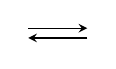
\begin{tikzpicture}[baseline] \draw[>=stealth,->] (0,1ex) -- (0.75,1ex); \draw[>=stealth,->] (0.75,0.25ex) -- (0,0.25ex); \end{tikzpicture}\ {#3}\thinspace\colon{#4}}

\renewcommand{\th}{\textsuperscript{th}}
\newcommand{\st}{\textsuperscript{st}}
\newcommand{\nd}{\textsuperscript{nd}}
\def\Cech{\v{C}ech}

% from http://tex.stackexchange.com/questions/41186/big-asterisk-bigast-symbol
% these are magic numbers that depend upon the other geometry options
\newcommand{\bigast}{\mathop{\scalebox{2.5}{\raisebox{-0.35ex}{$\ast$}}}}

% cf http://tex.stackexchange.com/questions/286050/rotated-math-with-correct-font-size for sizing instructions
\newcommand{\circulatearrows}{\text{$\curvearrowleft$\hspace{-0.95em}\rotatebox[origin=bl]{180}{$\curvearrowleft$}}}

\newcommand{\context}[1]{\mathcal{M}_{#1}}
\newcommand{\Ucontext}[1]{\mathcal{UM}_{#1}}
\newcommand{\Econtext}[1]{E_\infty\mathcal{M}_{#1}}
\newcommand{\CatOf}[1]{\mathsf{#1}}
\newcommand{\ps}[1]{\llbracket{#1}\rrbracket}
\newcommand{\moduli}[1]{\mathcal{M}_{\mathbf{#1}}}
\newcommand{\OS}[2]{\underline{\smash{#1}}_{#2}}
\newcommand{\InternalHom}[1]{\operatorname{\underline{\smash{\CatOf{#1}}}}}
\newcommand{\InternalAut}{\operatorname{\underline{\smash{\operatorname{Aut}}}}}
\newcommand{\InternalEnd}{\operatorname{\underline{\smash{\operatorname{End}}}}}
\newcommand{\sheaf}[1]{\mathcal{#1}}
\newcommand{\stack}[1]{\mathcal{#1}}
\newcommand{\ThomSheaf}[1]{\mathbb{L}(#1)}

\newcommand{\Spin}{\mathit{Spin}}
\newcommand{\String}{\mathit{String}}
\newcommand{\TMF}{\mathit{TMF}}
\newcommand{\Tmf}{\mathit{Tmf}}
\newcommand{\tmf}{\mathit{tmf}}
\renewcommand{\top}{\mathrm{top}}
\renewcommand{\ss}{\mathrm{ss}}
\newcommand{\ord}{\mathrm{ord}}
\newcommand{\alg}{\mathrm{alg}}
\newcommand{\ns}{\mathrm{ns}}
\newcommand{\TAF}{\mathit{TAF}}
\newcommand{\BP}{\mathit{BP}}
\newcommand{\MU}{\mathit{MU}}
\newcommand{\Tate}{\mathrm{Tate}}
\newcommand{\gl}{\mathit{gl}}
\newcommand{\GL}{\mathit{GL}}
\newcommand{\perf}{\mathrm{perf}}
\newcommand{\gpd}{\mathrm{gpd}}
\newcommand{\ptyp}{p\text{-}\mathrm{typ}}
\newcommand{\id}{\mathrm{id}}
\newcommand{\FGps}{\mathrm{FGps}}
\newcommand{\fin}{\mathrm{fin}}
\newcommand{\Res}{\mathrm{Res}}
\newcommand{\Tr}{\mathrm{Tr}}
\newcommand{\Cart}{\mathrm{Cart}}
\newcommand{\tr}{\mathrm{tr}}
\newcommand{\EinftyRings}{E_\infty\CatOf{RingSpectra}}

\DeclareMathOperator{\im}{im}
\DeclareMathOperator{\Ind}{Ind}
\DeclareMathOperator{\Spec}{Spec}
\DeclareMathOperator{\Spf}{Spf}
\DeclareMathOperator{\Sch}{Sch}
\DeclareMathOperator*{\colim}{colim}
\DeclareMathOperator{\End}{End}
\DeclareMathOperator{\Div}{Div}
\DeclareMathOperator{\SDiv}{SDiv}
\DeclareMathOperator{\Sq}{Sq}
\DeclareMathOperator{\Sym}{Sym}
\DeclareMathOperator{\Aut}{Aut}
\DeclareMathOperator{\Def}{Def}
\DeclareMathOperator{\Pic}{Pic}
\DeclareMathOperator{\Ext}{Ext}
\DeclareMathOperator{\hAut}{hAut}
\DeclareMathOperator{\Coord}{Coord}
\DeclareMathOperator{\Tor}{Tor}
\DeclareMathOperator{\Cotor}{Cotor}
\DeclareMathOperator{\coker}{coker}
\DeclareMathOperator{\Hom}{Hom}
\DeclareMathOperator{\Weil}{Weil}
\DeclareMathOperator{\Alt}{Alt}
\DeclareMathOperator{\Tot}{Tot}
\DeclareMathOperator{\height}{ht}
\DeclareMathOperator{\Sub}{Sub}
\DeclareMathOperator{\Level}{Level}
\DeclareMathOperator{\Mono}{Mono}
\DeclareMathOperator{\Isog}{Isog}
\DeclareMathOperator{\Td}{Td}
\DeclareMathOperator{\cofib}{cofib}
\DeclareMathOperator{\SpH}{SpH}
\DeclareMathOperator{\Lie}{Lie}
\DeclareMathOperator{\Frob}{Frob}
\let\div\undefined\DeclareMathOperator{\div}{div}

% theorem environments

\numberwithin{equation}{section}

\theoremstyle{plain}
\newtheorem{theorem}[equation]{Theorem}
\newtheorem{proposition}[equation]{Proposition}
\newtheorem{lemma}[equation]{Lemma}
\newtheorem{corollary}[equation]{Corollary}
\newtheorem{conjecture}[equation]{Conjecture}
\theoremstyle{definition}
\newtheorem{definition}[equation]{Definition}
\newtheorem{construction}[equation]{Construction}
\newtheorem{warning}[equation]{Important Warning}
\theoremstyle{remark}
\newtheorem{remark}[equation]{Remark}
\newtheorem{example}[equation]{Example}

% sseqpages definitions

\sseqnewgroup\tower[1]{
    \class(0,0)
    \foreach \y in {2,...,#1} {
        \class(0, \y-1)
        \structline(0, \y-2, -1)(0, \y-1, -1)
    }
}

\sseqnewcmd\etaclass{
    \class[class labels=above left,\options](\x,\y)
    \structline(\x-1,\y-1,-1)(\x,\y,-1)
}

% section headers

\crefname{section}{lecture}{lectures} \Crefname{section}{Lecture}{Lectures}
\crefname{chapter}{case study}{case studies} \Crefname{chapter}{Case Study}{Case Studies}

% put commas between adjacent footnotes without disturbing hyperref

\let\oldFootnote\footnote
\newcommand\nextToken\relax

\renewcommand\footnote[1]{%
    \oldFootnote{#1}\futurelet\nextToken\isFootnote}

\newcommand\isFootnote{%
    \ifx\footnote\nextToken\textsuperscript{,}%
    \else\ifx\footnotemark\nextToken\textsuperscript{,}\fi%
    \fi}

% from hood chatham: an \HFp macro that deals with subsequent subscripts intelligently

\makeatletter
\protected\def\HFp{H\mathbb{F}_p\@ifnextchar_{{}}{}}
\protected\def\HFtwo{H\mathbb{F}_2\@ifnextchar_{{}}{}}
\makeatother

% from hood chatham: place relevant spectral sequences on verso-recto pairs

\usepackage{afterpage}
\def\afterrectopage#1{\afterpage{\ifodd\thepage #1\else\afterpage{#1}\fi}}

% from hood chatham: an \intertext command that works in tikzcd

\usepackage{geometry}
\RequirePackage{tikz-cd}
\RequirePackage{etoolbox}

\usetikzlibrary{calc}
\edef\mytikzcdrestoreat{\catcode`@=\the\catcode`@\let\noexpand\mytikzcdrestoreat\noexpand\undefined}
\makeatletter
\newbox\mytikzcd@trialbox

\patchcmd\tikzcd@{#1]}{remember picture,#1]\let\intertext\mytikzcd@intertext}{}{\errorfailedtopatch}



\def\mytikzcd@addtosavedpaths#1{\xdef\tikzcd@savedpaths{\unexpanded\expandafter{\tikzcd@savedpaths}#1}}
\def\mytikzcd@intertext{
	\@ifnextchar[{\mytikzcd@intertext@}{\mytikzcd@intertext@[0pt]}
}

\def\mytikzcd@intertext@[#1]#2{
	\setbox\mytikzcd@trialbox=\vbox{\hsize\textwidth #2}
	\expandafter\\\expandafter[\the\dimexpr\ht\mytikzcd@trialbox+\dp\mytikzcd@trialbox+#1]
    \edef\mytikzcd@lmargin{\if@mparswitch\ifodd\thepage\space \Gm@lmargin\else \Gm@rmargin\fi\else \Gm@lmargin\fi}
    \@xp\mytikzcd@findcolumn\@xp{\tikzcd@savedpaths}{1}
	\mytikzcd@addtosavedpaths{\unexpanded{\path[overlay] let \p1=(current page.west), \p2 =} (\noexpand\tikzcdmatrixname-\the\numexpr\pgfmatrixcurrentrow-1\relax-\mytikzcd@column), \noexpand\p3 = (\noexpand\tikzcdmatrixname-\the\pgfmatrixcurrentrow-1) in
	node[anchor=west,text width=\textwidth,xshift=\mytikzcd@lmargin-2pt] at \unexpanded{(\x1,0.5*\y2+0.5*\y3)  {#2};}
	}
}


\def\mytikzcd@findcolumn#1#2{
    \def\mytikzcd@targetrow{#2}
    \expandafter\mytikzcd@findcolumn@\detokenize{#1\def\tikzcd@currentcolumn{x}\def\tikzcd@currentrow{6}}\@nil
}
\bgroup\lccode`\(=`\{\lccode`\)=`\}\lowercase{\egroup
\edef\mytikzcd@findcolumn@argspec{\unexpanded{#1}\detokenize{\def\tikzcd@currentcolumn}\unexpanded{(#2)}\detokenize{\def\tikzcd@currentrow}\unexpanded{(#3)}}
}

\@xp\def\@xp\mytikzcd@findcolumn@\mytikzcd@findcolumn@argspec{
    \expandafter\ifx\detokenize{x}#2
        \ifnum\mytikzcd@row<\the\numexpr\pgfmatrixcurrentrow-1\relax\def\mytikzcd@column{1}\fi
        \@xp\@gobbletonil
    \else
        \def\mytikzcd@column{#2}
        \def\mytikzcd@row{#3}
        \@xp\mytikzcd@findcolumn@
    \fi
}



\def\@gobbletonil#1\@nil{}
\mytikzcdrestoreat 

% from hood chatham: 

\makeatletter
\def\mathllap{\mathpalette\mathllapinternal}
\def\mathrlap{\mathpalette\mathrlapinternal}
\def\mathllapinternal#1#2{\llap{$\mathsurround=0pt#1{#2}$}}
\def\mathrlapinternal#1#2{\rlap{$\mathsurround=0pt#1{#2}$}}
\newtoks\sumfgl@toks
\newbox\sumfgl@box
\def\sumfgl{\sumfgl@toks{}\sumfgl@main}
\def\sumfgl@main#1{\@ifnextchar_{\sumfgl@sub{#1}}{\@ifnextchar^{\sumfgl@sup{#1}}{\mathpalette\sumfgl@done{#1}}}}
\def\sumfgl@sub#1_#2{\sumfgl@toks\expandafter{\the\sumfgl@toks_{#2}}\sumfgl@main{#1}}
\def\sumfgl@sup#1^#2{\sumfgl@toks\expandafter{\the\sumfgl@toks^{#2}}\sumfgl@main{#1}}
\def\sumfgl@done#1#2{
    \bgroup
    \setbox0=\hbox{$#1\sum\nolimits_{#2}\mskip1mu$}
    \global\setbox\sumfgl@box=\hbox{$\mathsurround=0pt#1\mathop{\sum\nolimits_{\mathrlap{#2}}}\limits\the\sumfgl@toks$}
    \ifdim\wd0>\wd\sumfgl@box \global\wd\sumfgl@box=\wd0 \fi
    \egroup
    \mathop{\box\sumfgl@box}
}
\def\sumphi{\sumfgl{\phi}}
\def\sumG{\sumfgl{\G}}
\def\sumGamma{\sumfgl{\Gamma}}
\makeatother




% from https://tex.stackexchange.com/questions/52076/how-to-make-a-superscript-on-the-upper-left-hand-corner-of-a-letter :

\def\presuper#1#2%
  {\mathop{}%
   \mathopen{\vphantom{#2}}^{#1}%
   \kern-\scriptspace%
   #2}

% from hood chatham: 
\makeatletter
\def\idxentry{\@ifnextchar[{\idxentry@}{\idxentry@dbl}}
% \def\idxentry@dbl#1{\mycommand@[#1]{#1}}
\def\idxentry@dbl#1{\textit{#1}\index{#1}}
\def\idxentry@[#1]#2{\textit{#2}\index{#1@#2}}
\makeatother


% if these change, be sure to update the pdf metadata in preamble.tex
\title[Lecture Notes]{Formal Geometry and Bordism Operations}
\author{Eric Peterson}
% \date{{\footnotesize Compiled: \today \\ Git hash: {\gitAbbrevHash}{\gitDirty}}}
\copyrightline{Copyright {\textcopyright} 2015--2017 Eric Peterson}



% --- REMOVE ME EVENTUALLY ---

\let\oldTodo\todo
\newcounter{todocounter}
\setcounter{todocounter}{0}
\renewcommand{\todo}{\addtocounter{todocounter}{1}\oldTodo}

% --- END REMOVE ME EVENTUALLY ---





\begin{document}

\bookabstract{We present various results in algebraic topology, primarily stemming from operations in bordism homology, in a unifying framework coming from algebraic geometry, primarily stemming from formal schemes.  This includes introductory presentations of chromatic homotopy theory and of elliptic cohomology.}
\bookkeywords{
55-01, % classroom textbook
55N22, % bordism homology
55N34, % elliptic homology
55P47, % infinite loopspaces
55R45, % homotopy and homology of BO, BU, ...
55S05, % primary operations
55S45, % Postnikov towers
55T15% the Adams SS
}

\frontmatter

\maketitle

% -*- root: main.tex -*-

% -*- root: main.tex -*-

\subsection*{Class information}

\vspace{2\baselineskip} \noindent \textit{Course ID: }
MATH 278 (159627).

\vspace{\baselineskip} \noindent \textit{Meeting times: }
Spring 2016, MWF 12pm--1pm.

\vspace{\baselineskip} \noindent \textit{Goals: }
The primary goal of this class is to teach students to view results in algebraic topology through the lens of (formal) algebraic geometry.

\vspace{\baselineskip} \noindent \textit{Grading: }
This class won't have any official assignments. I'll give references as readings for those who would like a deeper understanding, though I'll do my best to ensure that no extra reading is required to follow the arc of the class.

I do want to assemble course notes from this class, but it's unlikely that I will have time to type \emph{all} of them up. Instead, I would like to ``crowdsource'' this somewhat: I'll type up skeletal notes for each lecture, and then we as a class will try to flesh them out as the semester progresses. As incentive to help, those who contribute to the document will have their name included in the acknowledgements, and those who contribute \emph{substantially} will have their name added as a coauthor. Everyone could use more CV items. (Publication may take a while. I suspect the course won't run perfectly smoothly the first time, so this may takes a second semester pass to become fully workable. But, since topics courses only come around once in a while, this will necessarily mean a delay.)

The source for this document can be found at
\begin{center}
\texttt{https://github.com/ecpeterson/FormalGeomNotes}.
\end{center}
If you're taking the class or otherwise want to contribute, you can write me at
\begin{center}
\texttt{ecp@math.harvard.edu}
\end{center}
to request write access.

This document was compiled on \today. This may not reflect when it was cloned from git, though.\todo{I would like this to print the git HEAD's id, if it exists.  See https://www.ctan.org/tex-archive/macros/latex/contrib/gitinfo2 .}


\newpage

This document was compiled on \today. This may not reflect when it was cloned from git, though.\todo{I would like this to print the git HEAD's id, if it exists.  See https://www.ctan.org/tex-archive/macros/latex/contrib/gitinfo2 .}

\subsection*{Acknowledgements}

Matthew Ando, Michael Hopkins, Neil Strickland

Constantin Teleman

Haynes Miller, Doug Ravenel, Steve Wilson

Jack Morava

Nat Stapleton

Martin Bendersky



Hisham Sati: the \textit{Flavors of Cohomology} workshop

Berkeley students: Hood Chatham and Geoffrey Lee, Catherine Ray

Course participants (collected 2/3, probably missing some MIT people): Colin Aitken, Adam Al-Natsheh, Eva Belmont, Jason Bland, Dorin Boger, Lukas Brantner, Christian Carrick, Jun Hou Fung, Meng Guo, Jeremy Hahn, Changho Han, Chi-Yun Hsu, Erick Knight, Benjamin Landon, Gabriel Long, Yusheng Luo, Jack Marcinek, Jack McNamara, Max Menzies, Morgan Opie, Alexander Perry, Kishanu Sankar, Ananth Shankar, Danny Shi, Koji Shimizu, Geoffrey Smith, Hunter Spink, Philip Tynan, Yi Xie, David Yang, Zijian Yao, Lynnelle Ye, Chenglong Yu, Allen Yuan, Adrian Zahariuc, Yifei Zhao, Yihang Zhu.

People who contributed to the GitHub repository (to be collected later, make sure there's no overlap with the above list): 

Other readers: Jon Beardsley, Kevin Wray



\newpage
\tableofcontents

\todo[inline]{Make sure you use either $\id$ or $1$ everywhere to denote the identity morphism.}
\todo[inline]{You're not very consistent about using $\G$ or $\Gamma$ to denote an arbitrary formal group. It seems like you use one or the other based on your preference of whether it has finite height or not.}
\todo[inline]{Double check that you're careful about choosing consistent names for your objects: $S = \Spec R$ is the base scheme, that sort of thing.}
\todo[inline]{Be consistent about $\sheaf O_X$ vs $\sheaf O(X)$, and similarly with $\sheaf I_D$ versus $\sheaf I(D)$.}
\todo[inline]{Be consistent about ``$\S$'' versus ``$\S^0$'' for the standard sphere spectrum.}
\todo[inline]{We should use the convention that $\phi \in \moduli{fgl}(T)$ corresponds to $x +_\phi y \in T\ps{x, y}$ throughout.}
\todo[inline]{Be consistent about hyphens / en-dashes connecting ``$A$/$E$/$H_\infty$'' to ``ring''.}
\todo[inline]{Use $\EinftyRings$ everywhere appropriate.}
\todo[inline]{Use ${}^*$ and not ${}^\vee$ everywhere for linear dual.}
\todo[inline]{Make sure adjoint pairs are written with the left-adjoint on the left and with its arrow on top.}
\todo[inline]{Unify index entries.}
\todo[inline]{Make backreferences use cleveref.}
\todo[inline]{Get rid of the Appendix heading over the Bibliography.}




\mainmatter

% -*- root: main.tex -*-

\setcounter{chapter}{-1}
\chapter{Introduction}

\section{Introduction}\label{IntroductionSection}

The goal of this class is to communicate a certain \textit{weltanschauung} uncovered in pieces by many different people working in bordism theory, and the goal just for today is to tell a story about one theorem where it is especially apparent.

To begin, recall that a bordism theory $MX$, where $X$ is some suitable family of structure groups $X_n \to O(n)$, is a homology theory similar to singular homology but where the chains are constructed from $X$--structured manifolds and their boundaries.  The coefficient ring of $MX$, or its value $MX_*(*)$ on a point, gives the ring of $X$--bordism classes, and generally $MX_*(Y)$ of some space $Y$ gives a kind of ``bordism in families''.  There are evident comparison morphisms for the most ordinary kinds of bordism, given by replacing a chain of manifolds with an equivalent simplicial chain: \[MO \to H\Z/2, \quad MSO \to H\Z.\] In both cases, we can evaluate on a point to get ring maps $MO_*(*) \to \Z/2$ and $MSO_*(*) \to \Z$, called ``genera'' --- neither of which is very interesting, since they're both zero in positive degrees.\todo{A comparison of this with the usual spectrum definition of $MX$ appears in Switzer 12.35.}\todo{Jeremy thought spelling out the chain definition of bordism was helpful in understanding what was going on here.}

However, having maps of homology theories (rather than just maps of coefficient rings) is considerably more data: we can extact from this a theory of integration.  Consider the following:
\begin{align*}
MSO_n K(\Z, n) & = \left\{ \text{oriented $n$--manifolds mapping to $K(\Z, n)$} \right\} / \sim \\
& = \left\{ \begin{array}{c}\text{oriented $n$--manifolds $M$} \\ \text{with a specified class $\omega \in H^n(M; \Z)$} \end{array}\right\} / \sim.
\end{align*}
The yoga of stable homotopy theory then allows us to build a composite
\begin{align*}
\S^0 & \xrightarrow{\mathmakebox[2.5em]{(M, \omega)}} MSO \sm (\S^{-n} \sm \Susp^\infty_+ K(\Z, n)) \\ 
& \xrightarrow{\mathmakebox[2.5em]{\phantom{\phi}}} MSO \sm H\Z \\
& \xrightarrow{\mathmakebox[2.5em]{\phi \sm 1}} H\Z \sm H\Z \\
& \xrightarrow{\mathmakebox[2.5em]{\mu}} H\Z,
\end{align*}
where $\phi$ is the orientation map, and this gives us an integer. This integer is $\int_M \omega$, and it comes equipped with a Stokes' theorem due to the relation ``$\sim$'', and we can begin to see what the techniques of stable homotopy theory have to offer.

Now take $X = e$ to be the trivial structure group, so that the Pontryagin--Thom construction gives an equivalence $Me \xrightarrow{\simeq} \S$.  It is thus possible (and some people have indeed taken up this viewpoint) that stable homotopy theory can be done solely through the lens of ``framed bordism''. I'm a stable homotopy theorist rather than a differential topologist, and so I prefer to view this the other way: the sphere spectrum $\S$ often appears in my life as a natural object, and I will sometimes replace it by $Me$, the framed bordism spectrum.  For example, often I encounter a ring spectrum $E$, and it comes equipped with a unit map $\S \to E$, which I can reconsider as a ring map $\S = Me \to E$.  Following along the lines of the previous paragraph, we learn that we can thus think of any ring spectrum $E$ as automatically equipped with a theory of integration for framed manifolds.

Sometimes, as in the examples above, this unit map factors: \[\S = Me \to MO \to H\Z/2.\]  This is a witness to the overdeterminacy of $H\Z/2$'s integral for framed bordism: if the framed manifold is pushed all the way down to an unoriented manifold, there is still enough residual data to define the integral.  For a generic ring spectrum $E$, we can ask the analogous question: for a Hausdorff filtration on $O$ by structure groups, what stage does the unit map $Me \to E$ factor through?  The map $SO \to O$ considered above is the beginning of the Postnikov filtration of $O$, and we include a diagram of this filtration and some interesting integration theories related to it:
\begin{center}
\begin{tikzcd}
Me \arrow{r} \arrow{rrd} \arrow{rrrd} \arrow{rrrrd} & \cdots \arrow{r} & M\Spin \arrow{r} \arrow[crossing over]{d} & MSO \arrow{r} \arrow[crossing over]{d} & MO \arrow[crossing over]{d} \\
& & ko & H\Z & H\Z/2.
\end{tikzcd}
\end{center}

This is the situation homotopy theorists found themselves in some decades ago, in the wake of two important results of Ochanine and Witten. Ochanine had proven the following mysterious theorem using analytic techniques:

\begin{theorem}[Ochanine]
There is a cobordism invariant $o(M)$ of an oriented manifold $M$ which is a level $2$ modular form. It is somewhat multiplicative: if $F \to E \to M$ is an exceedingly nice fibration, then $o(E) = o(F) \cdot o(M)$.
\end{theorem}

\noindent Witten then strengthened this result considerably:

\begin{theorem}[Witten]
Ochanine's genus is in fact multiplicative. Also, if $M$ is a Spin manifold such that twice its first Pontryagin class vanishes, then $o(M)$ can be ``refined''\todo{What does ``refined'' mean, anyway? It's a square root, maybe?} to a level $1$ modular form $w(M)$.
\end{theorem}

\noindent However, neither party gave indication that their result should be valid ``in families'', and no theory of integration was produced.  It wasn't even clear what such a claim would mean: to give a topological enrichment of these theorems would mean finding a ring spectrum $E$ such that $E_*(*)$ had something to do with modular forms.  Around the same time, Landweber, Ravenel, and Stong began studying ``elliptic cohomology'' for independent reasons, and a decade later Ando, Hopkins, and Strickland put them together in the following theorem:

\begin{theorem}[Ando--Hopkins--Strickland]
If $E$ is an ``elliptic cohomology theory'', then there is a canonical map $M\String \to E$ called the $\sigma$--orientation.  Specializing to Tate $K$--theory $K^{\Tate}$, the induced map $M\String_* \to K^{\Tate}_*$ is Witten's genus.
\end{theorem}

We now come to the motivation for this class.  The homotopical $\sigma$--orientation was actually first constructed using formal geometry.  The original proof of Ando--Hopkins--Strickland begins with a reduction to understanding maps \[MU[6, \infty) \to E,\] and then they work to show that they can complete the missing arrow in the diagram
\begin{center}
\begin{tikzcd}
MU[6, \infty) \arrow{r} \arrow{rd} & M\String \arrow[densely dotted]{d} \\
& E.
\end{tikzcd}
\end{center}
Leaving aside the extension problem for the moment, their main theorem is the following description of the cohomology ring $E^* MU[6, \infty)$:
\begin{theorem}[Ando--Hopkins--Strickland]
For $E$ an even--periodic cohomology theory, \[\Spec E_* MU[6, \infty) \cong C^3(\G_E; \sheaf I(0)),\] where ``$C^3(\G_E; \sheaf I(0))$'' is a certain scheme.  When $E$ is taken to be elliptic, so that there is a specified isomorphism $\G_E \cong C^\wedge_0$ for $C$ an elliptic curve, this furnishes the scheme with a canonical point. Hence, there is a preferred class $MU[6, \infty) \to E$, natural in the choice of elliptic $E$.
\end{theorem}

\noindent Our real goal is to understand theorems like these.  The structure of the class will be, more or less, to work through a sequence of case studies where this perspective on algebraic topology shines through most brightly.  We'll start by working through Thom's calculation of the homotopy of $MO$, which simultaneously holds the attractive features of being free of technical complexity while revealing essentially all of the structural complexity.  Having seen that through to the end, we'll then work on reinforcing our technical underpinnings, and then we'll venture on to other examples.  The overriding theme of the class will be that this is a good organizing principle that gives us one avenue of insight into how homotopy theory functions.\todo{Mention not just what's to come but also what isn't. In particular, we're going to avoid $E_\infty$ geometry completely.}

\todo{Talk about existing resources here.  Be sure to mention Strickland's FSFG.}

\todo[inline]{Akhil wrote a couple of blog posts about Ochanine's theorem: \texttt{https://amathew.wordpress.com/2012/05/30/ochanines-theorem-on-elliptic-genera/} and \texttt{https://amathew.wordpress.com/2012/05/31/the-other-direction-of-ochaines-theorem/}. Mentioning a more precise result might lend to a more beefy introduction.}


% -*- root: main.tex -*-

\section*{Conventions}

Throughout this book, we use the following conventions:

\begin{itemize}
\item $\CatOf{C}(X, Y)$ will denote the mapping object of arrows $X \to Y$ in a category $\CatOf{C}$.  If $\CatOf{C}$ is an $\infty$--category, this will often be interpreted as a mapping \emph{space}.  If $\CatOf{C}$ has a self-enrichment, we will often write $\underline{\CatOf{C}}(X, Y)$ (or, e.g., $\InternalAut(X)$) to distinguish the internal mapping object from $\CatOf{C}(X, Y)$ the classical mapping set.
\item Following Lurie, for an object $X \in \CatOf C$ we will write $\CatOf C_{/X}$ for the slice category of objects \emph{over} $X$ and $\CatOf C_{X/}$ for the slice category of objects \emph{under} $X$.
\item For a ring spectrum $E$, we will write $E_* = \pi_* E$ for its coefficient ring, $E^* = \pi_{-*} E$ for its coefficient ring with the opposite grading, and $E_0 = E^0 = \pi_0 E$ for the $0${\th} degree component of its coefficient ring.  In particular, this allows us to make sense of expressions like ``$E^*\ps{x}$'', which we interpret as \[E^*\ps{x} = (E^*)\ps{x} = (\pi_{-*} E)\ps{x}.\]
\end{itemize}


\renewcommand\chaptername{Case Study}

% -*- root: main.tex -*-

\chapter{Unoriented bordism}


\section{Jan 27: Thom spectra and the Thom isomorphism}

Our first case study is a sequence of theorems about the unoriented bordism spectrum $MO$.  I wanted to begin by recalling one definition of the spectrum $MO$, since it involves ideas that will be useful to us throughout the semester.

\begin{definition}
For a spherical bundle $S^{n-1} \to \xi \to X$, its Thom space is given by the cofiber \[\xi \to X \xrightarrow{\text{cofiber}} T(\xi).\]
\end{definition}
\begin{proof}[``Proof'' of definition]
There's a more usual construction of the Thom space too: the associated disk bundle by gluing an $n$--disk in fiberwise, then taking the one--point compactification: \[T(\xi) = (\xi \sqcup'_{S^{n-1}} D^n)^+.\] How does this compare? Well, the thickening of $\xi$ is an $n$--disk bundle is the same thing as taking the mapping cylinder on $\xi \to X$. Since the inclusion into the mapping cylinder is now a cofibration, the quotient by this subspace agrees with both the cofiber of the map and the one--point compactification.
\end{proof}

Before proceeding, here are two important examples:
\begin{example}\label{TrivialBundleThomExample}
If $\xi = S^{n-1} \times X$ is the trivial bundle, then $T(\xi) = S^n \sm (X_+)$.  This is supposed to indicate what Thom spaces are ``doing'': if you feed in the trivial bundle then you get the suspension out, so if you feed in a twisted bundle you should think of it as a \textit{twisted suspension}.
\end{example}

\begin{example}\label{RPnThomExample}
Let $\xi$ be the tautological $S^0$--bundle over $\RP^\infty = BO(1)$.  Because $\xi$ has contractible total space, the cofiber degenerates and it follows that $T(\xi) = \RP^\infty$. More generally, arguing by cells shows that the Thom space for the tautological bundle over $\RP^n$ is $\RP^{n+1}$.
\end{example}

Now we catalog a bunch of useful properties of the Thom space functor. Firstly, recall that a spherical bundle over $X$ is the same data as a map $X \to B \GL_1 S^{n-1}$, where $\GL_1 S^{n-1}$ is the subspace of $F(S^{n-1}, S^{n-1})$ expressed by the pullback
\begin{center}
\begin{tikzcd}
\GL_1 S^{n-1} \arrow{r} \arrow{d} & F(S^{n-1}, S^{n-1}) \arrow{d} \\
\Aut_{h\CatOf{Spaces}} S^{n-1} \arrow{r} & \End_{h\CatOf{Spaces}} S^{n-1} \arrow[-,double]{r} & \pi_0 F(S^{n-1}, S^{n-1}).
\end{tikzcd}
\end{center}
We can interpret $T$ as a functor from the slice category over $BGL_1 S^{n-1}$ to $\CatOf{Spaces}$: maps \[Y \xrightarrow{f} X \xrightarrow{\xi} B \GL_1 S^{n-1}\] induce maps $T(f^* \xi) \to T(\xi)$, and $T$ is suitably homotopy-invariant.

Next, a common source of spherical bundles is taking the spherical subbundle of a vector bundle.  Since rank $n$ vector bundles are also classified by an object $BO(n)$, this begets a map $J_{\R}^n: BO(n) \to B \GL_1 S^{n-1}$ for each $n$.  Homotopy theorists are very interested in the block--inclusion maps $i^n: BO(n) \to BO(n+1)$ and the colimit $BO = BO(\infty)$.  The suspension functor induces a map $\GL_1 S^{n-1} \to \GL_1 S^n$, and we are led to ask about the compatibility of these operations.  As a route to answering this, the block--inclusion maps are a special case of a more general direct sum map $\oplus: BO(n) \times BO(m) \to BO(n+m)$, given by the precomposition \[BO(n) = BO(n) \times * \xrightarrow{\operatorname{id} \times \text{triv}} BO(n) \times BO(1) \xrightarrow\oplus BO(n+1).\] The spaces $B \GL_1 S^{n-1}$ enjoy a similar ``collective monoid'' structure, given by taking the fiberwise join two spherical bundles with a common base.
\begin{lemma}
The fiberwise join is represented by maps \[B\GL_1 S^{n-1} \times B\GL_1 S^{m-1} \to B\GL_1 S^{n+m-1},\] and these maps commute with the block sum maps on the $BO(n)$ family. \qed
\end{lemma}
\noindent Again taking a cue from $K$--theory, we take the colimit as $n$ grows large.
\begin{corollary}
There is a map of $H$--spaces $J_{\R}: BO \to B\GL_1 \S$ called the \textit{stable $J$--homomorphism}. \qed
\end{corollary}
\noindent Finally, we can ask about the compatibility of $T$ with all of this:
\begin{lemma}
$T$ is monoidal: it carries fiberwise joins to smash products of spaces. \qed
\end{lemma}

We are now prepared to define our spectrum $MO$.  The unstable $J$--maps $J_{\R}^n: BO(n) \to B\GL_1 S^{n-1}$ give Thom spaces $T(J_{\R}^n)$,\todo{Be careful about dimension here: you really mean a reduced tautological bundle, related to how $BO$ has only one connected component.} equipped with maps\todo{Fix this equation.} \[\Susp T(J_{\R}^n) = T(J_{\R}^n \oplus \text{triv}) \to T(J_{\R}^{n+1}).\] Setting $MO(n) = \Susp^{-n} \Susp^\infty T(J_{\R}^n)$, we again assemble this data into a single object: \[MO := \colim_n MO(n) = \colim_n \Susp^{-n} T(J_{\R}^n).\]

The spectrum $MO$ has several remarkable properties.  The most basic such property is that it is a ring spectrum, and this follows immediately from $J_{\R}$ being a homomorphism of $H$--spaces.  Much more excitingly, we can also deduce the presence of Thom isomorphisms just from the properties stated thus far.  That $J_{\R}$ is a homomorphism means that the following square commutes:
\begin{center}
\begin{tikzcd}
BO \times BO \arrow{r}{\sigma, \simeq} \arrow[bend right]{rrd} & BO \times BO \arrow{r}{\mu} \arrow{d}{J_{\R} \times J_{\R}} & BO \arrow{d}{J_{\R}} \\
& B\GL_1 \S \times B\GL_1 \S \arrow{r}{\mu} & B\GL_1 \S.
\end{tikzcd}
\end{center}
We have extended this square very slightly by a certain shearing map $\sigma$ defined by $\sigma(x, y) = (xy^{-1}, y)$.\todo{$\sigma$ \emph{almost} shows up in giving a categorical definition of a $G$--torsor.  I wish I understood this, but I always get tangled up.}  It's evident that $\sigma$ is a homotopy equivalence, since just as we can de-scale the first coordinate by $y$ we can re-scale by it.  We can calculate directly the behavior of the long composite: \[J_{\R} \circ \mu \circ \sigma(x, y) = J_{\R} \circ \mu(xy^{-1}, y) = J_{\R}(xy^{-1}y) = J_{\R}(x).\]  It follows that the second coordinate plays no role, and that the bundle classified by the long composite can be written as $J_{\R} \times 0$.\footnote{This factorization does \emph{not} commute with the rest of the diagram, just with the little triangle it forms.}  We are now in a position to see the Thom isomorphism:
\begin{lemma}[Thom isomorphism, universal example] $MO \sm MO \simeq MO \sm \Susp^\infty_+ BO$.\todo{Is it clear that this is an equivalence of $MO$--modules? This should come from the $x$--factor being unmolested, right?}\todo{Is it furthermore clear that the cohomological version of this gives an action of $E^* X$ on $E^* T(\xi)$ by the ``Thom diagonal''?}
\end{lemma}
\begin{proof}
Stringing together the naturality properties of the Thom functor outlined above, we can thus make the following calculation:\todo{This Q.E.D.\ block isn't typeset well.}
\begin{align*}
T(\mu \circ (J_{\R} \times J_{\R})) & \simeq T(\mu \circ (J_{\R} \times J_{\R}) \circ \sigma) & \text{(homotopy invariance)} \\
& \simeq T(\mu \circ (J_{\R} \times 0)) & \text{(constructed lift)} \\
& \simeq T(J_{\R}) \sm T(0) & \text{(monoidality)} \\
& \simeq MO \sm \Susp^\infty_+ BO & \text{(definition of $MO$, \Cref{TrivialBundleThomExample})} \\
T(J_{\R}) \sm T(J_{\R}) & \simeq MO \sm \Susp^\infty_+ BO & \text{(monoidality)} \\
MO \sm MO & \simeq MO \sm \Susp^\infty_+ BO. & \text{(definition of $MO$) \qedhere}
\end{align*}
\end{proof}

From here, the general version of Thom's theorem follows quickly:
\begin{theorem}[Thom isomorphism]
Let $\xi: X \to BO$ classify a vector bundle and let $\phi: MO \to E$ be a map of ring spectra. Then there is an equivalence of $E$--modules \[E \sm T(\xi) \simeq E \sm \Susp^\infty_+ X.\]
\end{theorem}
\begin{proof}[Modifications to above proof]
To accommodate $X$ rather than $BO$ as the base, we redefine $\sigma: BO \times X \to BO \times X$ by \[\sigma(x, y) = \sigma(x \xi(y)^{-1}, y).\]  This gives an equivalence $MO \sm T(\xi) \simeq MO \sm \Susp^\infty_+ X$.  To introduce $E$, note that there is a diagram
\begin{center}
\begin{tikzcd}
E \sm T(\xi) \arrow[densely dotted]{r}{\simeq} \arrow{d}{\eta_{MO} \sm \id \sm \id} & E \sm \Susp^\infty_+ X \arrow{d}{\eta_{MO} \sm \id \sm \id} \\
MO \sm E \sm T(\xi) \arrow{r}{\simeq} \arrow{d}{(\mu \circ (\phi \sm \id)) \sm \id} & MO \sm E \sm \Susp^\infty_+ X \arrow{d}{(\mu \circ (\phi \sm \id)) \sm \id} \\
E \sm T(\xi) \arrow{r} & E \sm \Susp^\infty_+ X.
\end{tikzcd}
\end{center}
The middle equivalence comes from the previous Thom isomorphism, smashed through with $E$.  The bottom arrow exists by applying the action map to both sides.  Reusing the bottom arrow at the top arrow and using the unitality of the monoid $E$ shows the map to be an equivalence.
\end{proof}

We'll close out today by using this to actually make a calculation of something. Recall from \Cref{RPnThomExample} that $T(\L - 1 \downarrow \RP^n) = \RP^{n+1}$.  By killing all the homotopy elements in positive degrees, you can also see that the map $MO \to MO(-\infty, 0] = H\Z/2$ is a ring map\todo{This requires some justification, like $MO$ being connective.}, so that we can apply the Thom isomorphism theorem to the mod--$2$ homology of Thom complexes coming from real vector bundles:
\begin{align*}
\pi_* (H\Z/2 \sm T(\L - 1)) & \cong \pi_* (H\Z/2 \sm T(0)) & \text{(Thom isomorphism)} \\
\pi_* (H\Z/2 \sm \Susp^{-1} \Susp^\infty \RP^{n+1}) & \cong \pi_* (H\Z/2 \sm \Susp^\infty_+ \RP^n) & \text{(\Cref{RPnThomExample})} \\
\widetilde{H\Z/2}_{*+1} \RP^{n+1} & \cong H\Z/2_* \RP^n. & \text{(generalized homology)}
\end{align*}
This powers an induction that shows that $H\Z/2_* \RP^\infty$ has a single class in every degree.\todo{Using the cohomology version of this together with the $H\Z/2^* \RP^n$--module structure of $H\Z/2^* T(\L-1)$ deduces the ring structure too.}






\section{Jan 29: Cohomology rings and affine schemes}

\todo{Decide on $\Z/2$ versus $\F_2$. I think in the previous lecture you were avoiding $\F_2$ because it got in the way of your homology subscripts.}An abbreviated summary of this semester is that we're going to put ``$\Spec$'' in front of rings appearing in algebraic topology and see what happens.  Before doing any algebraic topology, let me remind you what this means on the level of algebra.  The core idea is to replace a ring $R$ by the functor it corepresents.  For any ``test $\F_2$--algebra'' $T$, we set \[\Spec(R)(T) := \CatOf{Schemes}_{/\F_2}(\Spec T, \Spec R) := \CatOf{Algebras}_{\F_2/}(R, T).\]  More generally, we have the following definition:
\begin{definition}
An \textit{affine $\F_2$--scheme} is a functor $X: \CatOf{Algebras}_{\F_2/} \to \CatOf{Sets}$ which is (noncanonically) isomorphic to $\Spec R$ for some $\F_2$--algebra $R$.  Given such an isomorphism, we will refer to $\Spec R \to X$ as a \textit{parameter} for $X$ and its inverse $X \to \Spec R$ as a \textit{coordinate} for $X$.
\end{definition}

\begin{lemma}
There is an equivalence of categories \[\Spec: \CatOf{Algebras}_{\F_2/}^{\mathrm{op}} \to \CatOf{AffineSchemes}_{/\F_2}. \qed\]
\end{lemma}

The centerpiece of thinking about rings in this way is to translate between a presentation of $R$ as a quotient of a free algebra and a presentation of $(\Spec R)(T)$ as selecting tuples of elements in $T$ subject to certain conditions.  Consider the following example:
\begin{example}
Set $R_1 = \F_2[x]$.  Then \[(\Spec R_1)(T) = \CatOf{Algebras}_{\F_2/}(\F_2[x], T)\] is determined by where $x$ is sent --- i.e., this Hom--set is naturally isomorphic to $T$ itself.  Consider also what happens when we impose a relation by passing to $R_2 = \F_2[x] / (x^{n+1})$.  The value \[(\Spec R_2)(T) = \CatOf{Algebras}_{\F_2/}(\F_2[x] / (x^{n+1}), T)\] of the associated affine scheme is again determined by where $x$ is sent, but now $x$ can only be sent to elements which are nilpotent of order $n+1$.  These schemes are both important enough that we give them special names:
\begin{align*}
\mathbb A^1 & := \Spec \F_2[x], & \mathbb A^{1, (n)} & := \Spec \F_2[x] / (x^{n+1}).
\end{align*}
The symbol ``$\mathbb A^1$'' is pronounced ``the affine line''.  Note that the quotient map $R_1 \to R_2$ induces an inclusion $\mathbb A^{1, (n)} \to \mathbb A^1$ and that $\mathbb A^{1, (0)}$ is a constant functor: \[\mathbb A^{1, (0)}(T) = \{f: \F_2[x] \to T \mid f(x) = 0\}.\]  Accordingly, we pronounce ``$\mathbb A^{1, (0)}$'' as ``the origin on the affine line'' and ``$\mathbb A^{1, (n)}$'' as ``the $n${\th} order neighborhood of the origin in the affine line''.
\end{example}

We can also express in this language another common object in algebraic topology: the Hopf algebra, which arises when taking the mod--$2$ cohomology of an $H$--space.  In addition to the usual cohomology, the extra pieces of data are those induced by the $H$--space multiplication and unit map, which on cohomology beget a diagonal map $\Delta$ and an antipode map $\chi$.  Running through the axioms, one quickly checks the following:
\begin{lemma}
For a Hopf $\F_2$--algebra $R$, the functor $\Spec R$ is naturally valued in groups.  Such functors are called \textit{group schemes}.  Conversely, a choice of group structure on $(\Spec R)(T)$ natural in $T$ endows $R$ with the structure of a Hopf algebra. \todo{Maybe write this out, if you're going to be using this equivalence all semester.} \qed
\end{lemma}

\begin{example}\label{InformalAdditiveGroupExample}
The functor $\mathbb A^1$ introduced above is naturally valued in groups: since $\mathbb A^1(T) \cong T$, we can use the addition on $T$ to make it into an abelian group.  When considering $\mathbb A^1$ with this group scheme structure, we notate it as $\mathbb G_a$.  Applying the Yoneda lemma, one deduces the following formulas for the Hopf algebra structure maps:
\begin{align*}
\mathbb G_a \times \mathbb G_a & \xrightarrow{\mu} \mathbb G_a & x_1 + x_2 & \mapsfrom x, \\
\mathbb G_a & \xrightarrow{\chi} \mathbb G_a & -x & \mapsfrom x, \\
\Spec \F_2 & \xrightarrow{\eta} \mathbb G_a & 0 & \mapsfrom x.
\end{align*}
\end{example}

\begin{remark}
In fact, $\mathbb A^1$ is naturally valued in \emph{rings}. It models the inverse functor to $\Spec$ in the equivalence of categories above, i.e., the elements of a ring $R$ always form a complete collection of coordinates on some affine scheme $\Spec R$.
\end{remark}

\begin{example}
We define the \textit{multiplicative group scheme} by\todo{Do you want this to be a $\Z$--algebra? Ditto with $\mathbb A^1$ and $\mathbb G_a$?} \[\mathbb G_m = \Spec \F_2[x, y] / (xy - 1).\]  Its value $\mathbb G_m(T)$ on a test algebra $T$ is the set of pairs $(x, y)$ such that $y$ is a multiplicative inverse to $x$, and hence $\mathbb G_m$ is valued in groups.  Applying the Yoneda lemma, we deduce the following formulas for the Hopf algebra structure maps:
\begin{align*}
\mathbb G_m \times \mathbb G_m & \xrightarrow{\mu} \mathbb G_m & x_1 \otimes x_2 & \mapsfrom x \\
& & y_1 \otimes y_2 & \mapsfrom y, \\
\mathbb G_m & \xrightarrow{\chi} \mathbb G_m & (y, x) & \mapsfrom (x, y), \\
\Spec R & \xrightarrow{\eta} \mathbb G_m & 1 & \mapsfrom x, y.
\end{align*}
\end{example}

\begin{remark}
As presented above, $\mathbb G_m$ comes with a natural inclusion $\mathbb G_m \to \mathbb A^2$.  However, the coordinate $x$ on $\mathbb G_m$ gives a map $x: \mathbb G_m \to \mathbb A^1$, and because multiplicative inverses in a ring are unique, we see that this map is also an inclusion.  These two inclusions have rather different properties, and we'll think harder about their essential differences later on.
\end{remark}

Let's now consider the example that we closed with last time, where we calculated $H\Z/2^*(\RP^n) = \F_2[x] / (x^{n+1})$.  Putting ``$\Spec$'' in front of this, we could reinterpret this calculation as \[\Spec H\F_2^*(\RP^n) \cong \mathbb A^{1, (n)}.\]  This is such a useful thing to do that we will give it a notation all of its own:

\begin{definition}
Let $X$ be a finite cell complex, so that $H\F_2^*(X)$ is a ring which is finite--dimensional as an $\F_2$--vector space.  We will write \[X_{H\F_2} = \Spec H\F_2^* X\] for the corresponding finite affine scheme.
\end{definition}

\begin{example}
Putting together the discussions from this time and last time, in the new notation we have calculated \[\RP^n_{H\Z/2} \cong \mathbb A^{1, (n)}.\]
\end{example}

So far, this example just restates things we knew in a mildly different language.  Our driving goal for the remainder of today and for tomorrow is to incorporate as much information as we have about these cohomology rings $H\F_2^* \RP^n$ into this description, which will result in us giving a more ``precise'' name for this object.  Along the way, we will discover why $X$ had to be a \emph{finite} complex and how to think about more general $X$.  For now, though, let's content ourselves with investigating the Hopf algebra structure on $H\F_2^* \RP^\infty$.

\begin{example}\label{RPExampleFaulty}
Recall that $\RP^\infty$ is an $H$--space in two equivalent ways:
\begin{enumerate}
\item There is an identification $\RP^\infty \simeq K(\Z/2, 1)$, and the $H$--space structure is induced by the sum on cohomology.
\item There is an identification $\RP^\infty \simeq BO(1)$, and the $H$--space structure is induced by the tensor product of real line bundles.
\end{enumerate}
In both cases, this induces a Hopf algebra diagonal \[H\F_2^* \RP^\infty \otimes H\F_2^* \RP^\infty \xleftarrow\Delta H\F_2^* \RP^\infty\] which we would like to analyze.  This map is determined by where it sends the class $x$, and because it must simultaneously respect gradings it must be of the form $\Delta x = ax_1 + bx_2$ for some constants $a, b \in \F_2$.  Furthermore, because it belongs to a Hopf algebra structure, it must satisfy the unitality axiom
\begin{center}
\begin{tikzcd}
H\F_2^* \RP^\infty \arrow[leftarrow]{r}{\begin{array}{c} \epsilon \otimes \id \\ \id \otimes \epsilon \end{array}} \arrow[leftarrow, bend right]{rr}{\id} & H\F_2^* \RP^\infty \otimes H\F_2^* \RP^\infty \arrow[leftarrow]{r}{\Delta} & H\F_2^* \RP^\infty.
\end{tikzcd}
\end{center}
and hence it takes the form \[\Delta(x) = x_1 + x_2.\]  Noticing that this is exactly the diagonal map in \Cref{InformalAdditiveGroupExample}, we tentatively identify ``$\RP^\infty_{H\F_2}$'' with the additive group.  This is extremely suggestive but does not take into account the fact that $\RP^\infty$ is an infinite complex, so we haven't allowed ourselves to write ``$\RP^\infty_{H\F_2}$'' just yet.  We will straighten this out tomorrow.
\end{example}








\section{Feb 1: The Steenrod algebra}


We left off yesterday complaining that our definition was only made for finite complexes, and that this was getting in the way of a nice theorem.  However, had we naively defined $X_{H\F_2}$ for infinite complexes $X$, we would have quickly seen that we would have gotten ``the wrong answer'' for several $X$.  Without going into detail yet about the bad examples we're trying to avoid, it will turn out that we can fix them by rigidifying the target category somewhat.  Here are the extra structures we will work toward incorporating, some quickly and some slowly:
\begin{enumerate}
\item Cohomology rings are \emph{graded}, and maps of spaces respect this grading.
\item Cohomology rings receive an action of the Steenrod algebra, and maps of spaces respect this action.
\item Both of these are complicated further when taking the cohomology of an infinite complex.
\item \label{SkewCommutativeDeficiency} (Cohomology rings for more elaborate cohomology theories are only skew-commutative, but ``$\Spec$'' requires a commutative input.)
\end{enumerate}
Today we will fix all these deficiencies of $X_{H\F_2}$ except for \#\ref{SkewCommutativeDeficiency}, which doesn't matter with mod--$2$ coefficients but which will be something of a bugbear throughout the rest of the semester.

Let's begin by considering the grading on $H\F_2^* X$.  There is a standard construction in algebraic geometry that tracks gradings, which we now recall:

\begin{definition}\todo{Cite: Strickland FSFG, Defn 2.95.}
A \textit{grading} on a ring $R$ is a system of additive subgroups $R_k$ of $R$ satisfying $R = \bigoplus_k R_k$, $1 \in R_0$, and $R_j R_k \subseteq R_{j+k}$.  Additionally, a map $f: R \to S$ of graded rings is said to be \textit{homogeneous} or to \textit{respect the grading} if $f(R_k) \subseteq S_k$.
\end{definition}

\begin{lemma}\label{GradedAndGmEquivAgree}\todo{Cite this: Strickland FSFG, Prop 2.96.}
A graded ring $R$ is equivalent data to an affine scheme $\Spec R$ with an action by $\mathbb G_m$.  Additionally, a map $R \to S$ is homogeneous exactly when the induced map $\Spec S \to \Spec R$ is $\mathbb G_m$--equivariant.
\end{lemma}
\begin{proof}
A $\mathbb G_m$--action on $\Spec R$ is equivalent data to a coaction map $\alpha^*: R \to R \otimes \F_2[x^\pm]$.  Define $R_k$ to be those points in $r$ satisfying $\alpha^* r = r \otimes x^k$.  It is clear that we have $1 \in R_0$ and that $R_j R_k \subseteq R_{j+k}$.  To see that $R = \bigoplus_k R_k$, note that every tensor can be written as a sum of pure tensors.  Conversely, given a graded ring $R$, define the coaction map on $R_k$ by \[(r_k \in R_k) \mapsto x^k r_k\] and extend linearly.
\end{proof}

This notion from algebraic geometry is somewhat different from what we are used to in algebraic topology, as it is designed to deal with things like polynomial rings, but in classical algebraic topology we only ever encounter homogeneous sums.  We can modify our perspectively very slightly to arrive at the algebraic geometers': replace $H\F_2$ by the periodified spectrum \[H\F_2P = \bigvee_{j=-\infty}^\infty \Susp^j H\F_2.\]  This spectrum has the property that $H\F_2P^0(X)$ is isomorphic to $H\F_2^*(X)$ as ungraded rings, but now we can make sense of the sum of two classes which used to live in different $H\F_2$--degrees.  At this point we can manually craft the desired coaction map $\alpha^*$ so that we are in the situation of \Cref{GradedAndGmEquivAgree}, but we will shortly find that algebraic topology gifts us with it on its own.

Our route to finding this natural $\alpha^*$ is by turning to the next extra structure: the action of the Steenrod algebra.  Naively approached, this does not fit into the framework we've been sketching so far: the Steenrod algebra is a noncommutative algebra, and so the action map \[\mathcal A^* \otimes H\F_2^* X \to H\F_2^* X\] will be difficult to squeeze into any kind of algebro-geometric framework.  Milnor was the first person to see a way around this, with two crucial observations.  First, the linear-algebraic dual of the Steenrod algebra $\mathcal A_*$ is a commutative ring, since the Cartan formula expressing the diagonal on $\mathcal A^*$ is evidently symmetric.  Second, if $X$ is a \emph{finite} complex, then tinkering with Spanier--Whitehead duality gives rise to a map: \[\mathcal A^* \otimes (H\F_2)_* X \to (H\F_2)_* X.\]  Applying linear-algebraic duality to this bottom map allows us to reinterpret this as a coaction map \[\lambda^*: H\F_2^* X \to H\F_2^* X \otimes \mathcal A_*,\] which we will then re-re-interpret as an action map \[\alpha: \Spec \mathcal A_* \times X_{H\F_2} \to X_{H\F_2}.\]  Milnor works out the Hopf algebra structure of $\mathcal A_*$, by defining elements $\xi_j \in \mathcal A_*$ dual to $\Sq^{2^{j-1}} \cdots \Sq^{2^0} \in \mathcal A^*$.  Taking $X = \RP^n$ and $x \in H\F_2^1(\RP^n)$ the generator, then since $\Sq^{2^{j-1}} \cdots \Sq^{2^0} x = x^{2^j}$ he deduces the formula \[\lambda^*(x) = \sum_{j=0}^{\lfloor \log_2 n \rfloor} x^{2^j} \otimes \xi_j.\]  Notice that we can take the limit $n \to \infty$ if we aren't afraid of infinite sums.  He then makes the following calculation, stable in $n$:
\begin{align*}
(\lambda^* \otimes \id) \circ \lambda^*(x) & = (\id \otimes \Delta) \circ \lambda^*(x) & \text{(coaction)} \\
(\lambda^* \otimes \id) \left( \sum_{j=0}^\infty x^{2^j} \otimes \xi_j \right) & = \\
\sum_{j=0}^\infty \left( \sum_{i=0}^\infty x^{2^i} \otimes \xi_i \right)^{2^j} \otimes \xi_j & = & \text{(ring homomorphism)} \\
\sum_{j=0}^\infty \left( \sum_{i=0}^\infty x^{2^{i+j}} \otimes \xi_i^{2^j} \right) \otimes \xi_j & = & \text{(characteristic $2$)} \\
\sum_{j=0}^\infty \left( \sum_{i=0}^\infty x^{2^{i+j}} \otimes \xi_i^{2^j} \right) \otimes \xi_j & = (\id \otimes \Delta) \left( \sum_{m=0}^\infty x^{2^m} \otimes \xi_m \right) \\
\sum_{j=0}^\infty \left( \sum_{i=0}^\infty x^{2^{i+j}} \otimes \xi_i^{2^j} \right) \otimes \xi_j & = \sum_{m=0}^\infty x^{2^m} \otimes \Delta(\xi_m),
\end{align*}
from which it follows that \[\Delta \xi_m = \sum_{i+j=m} \xi_i^{2^j} \otimes \xi_j.\]  Finally, Milnor shows that this is the complete story:
\begin{theorem}[Milnor]
$\mathcal A_* = \F_2[\xi_1, \xi_2, \ldots, \xi_j, \ldots]$.
\end{theorem}
\begin{proof}[Flippant proof]
Milnor counts how many elements he has produced, compares against how many Adem and Cartan found, and sees that he has exactly enough.
\end{proof}

We are now in a position to uncover the desired map $\alpha^*$ desired earlier.  Suppose that we were interested in re-telling Milnor's story with $H\F_2P$ in place of $H\F_2$.  The dual Steenrod algebra is defined by \[\mathcal A_* := \pi_*(H\F_2 \sm H\F_2),\] which we replace by \[\mathcal AP_0 := \pi_0 (H\F_2 P \sm H\F_2 P) = H\F_2P_0(H\F_2) = \mathcal A_*[\xi_0^\pm].\]  Restricting to the quotient Hopf algebra $\mathcal AP_0 \to \F_2[\xi_0^\pm]$ gives exactly the coaction map $\alpha^*$.

To study the rest of $\mathcal AP_0$ in terms of algebraic geometry, we need only identify what the series $\lambda^*(x)$ embodies.  Note that this necessarily involves some creativity, and the only justification we can supply will be moral, borne out over time.  With that caveat in mind, here is one such description.  Recall the map induced by the $H$--space multiplication \[H\F_2^* \RP^\infty \otimes H\F_2^* \RP^\infty \leftarrow H\F_2^* \RP^\infty.\]  Taking a colimit over finite complexes, we produce an coaction of $\mathcal A_*$, and since the map above comes from a map of spaces, it is equivariant for the coaction.  Since the action on the left is diagonal, we deduce the formula \[\lambda^*(x_1 + x_2) = \lambda^*(x_1) + \lambda^*(x_2).\]

\begin{lemma}
The series $\lambda^*(x) = \sum_{j=0}^\infty x^{2^j} \otimes \xi_j$ is the universal example of a series satisfying $\lambda^*(x_1 + x_2) = \lambda^*(x_1) + \lambda^*(x_2)$.  The value $(\Spec \mathcal AP_0)(T)$ is the set of power series $f$ with coefficients in $T$ satisfying \[f(x_1 + x_2) = f(x_1) + f(x_2). \qed\]
\end{lemma}

We close our discussion by codifying what Milnor did when he stabilized against $n$.  Each $\RP^n_{H\F_2}$ is a finite affine scheme, and to make sense of the object $\RP^\infty_{H\F_2}$ Milnor's technique was to consider the ind-system $\{\RP^n_{H\F_2}\}_{n=0}^\infty$ of finite affine schemes.  We give a name to these sorts of objects:\todo{Maybe move formal schemes into the previous lecture and talk about completions too?}
\begin{definition}
An \textit{affine formal scheme} is an ind-system of finite affine schemes.
\end{definition}
\noindent We will follow this technique ourselves to handle general infinite complexes:
\begin{definition}
When $X$ is an infinite complex, filter it by its subskeleta $X^{(n)}$ and define $X_{H\F_2}$ to be the ind-system $\{X^{(n)}_{H\F_2}\}_{n=0}^\infty$ of finite schemes.
\end{definition}

This choice clarifies the example from last time:
\begin{example}[{cf. \Cref{RPExampleFaulty}}]\label{RPinftyExampleForReal}
Write $\G_a$ for the ind-system $\mathbb A^{1, (n)}$ with the group scheme structure given in \Cref{RPExampleFaulty}.  That this group scheme structure filters this way is a simultaneous reflection of two facts:
\begin{enumerate}
\item $\G_a(T)$ consists of all nilpotent elements in $T$.  The sum of two nilpotent elements of orders $n$ and $m$ is guaranteed to itself be nilpotent with order at most $n+m$.
\item There is a skeletal factorization of the multiplication map on $\RP^\infty$ as $\RP^n \times \RP^m \to \RP^{n+m}$ purely for dimensional reasons.\todo{Is there an off-by-one here?}
\end{enumerate}
As group schemes, we have calculated \[\RP^\infty_{H\F_2} \cong \G_a.\]
\end{example}

Additionally, this choice allows us to give a name to $\Spec \mathcal AP_0$.  Note that the following morphism sets are very different:
\begin{align*}
\CatOf{GroupSchemes}_{/\F_2}(\mathbb G_a, \mathbb G_a) & \cong \CatOf{HopfAlgebras}_{\F_2/}(\F_2[x], \F_2[x]) \\
\CatOf{FormalGroups}_{/\F_2}(\G_a, \G_a) & \cong \CatOf{HopfProAlgebras}_{\F_2/}(\F_2\llbracket x \rrbracket, \F_2\llbracket x \rrbracket).
\end{align*}
The former is populated by polynomials satisfying the homomorphism condition and the latter is populated by power series satisfying the homomorphism condition.  Since our description of $\Spec \mathcal AP_0$ involves power series, we can amp up this observation to a scheme: \[\underline{\operatorname{Hom}}(X, Y)(T) = \left\{ (u, f) \middle| \begin{array}{c} u: \Spec T \to \Spec \F_2, \\ f: u^* X \to u^* Y \end{array}\right\}\] and conclude that the correct name for $\Spec \mathcal AP_0$ is \[\Spec \mathcal AP_0 \cong \underline{\Aut}(\G_a).\]

Finally, the formula $\RP^\infty_{H\F_2} \cong \G_a$ is meant to point out that this language of formal schemes has an extremely good compression ratio: you can fit a lot of information into a very tiny space.  This formula simultaneously embodies the cohomology ring of $\RP^\infty$, its diagonal, and how the dual Steenrod algebra coacts.

\todo{Include a recursive formula for the antipode map, coming from power series inversion.}






\section{Feb 3: Comodule cohomology I: Group cohomology}

\todo{This section is written gradedly and probably shouldn't be, for consistency.} Today we'll focus on an important classical tool: the Adams spectral sequence.  We're going to study this in greater earnest later on, so I will avoid giving a satisfying construction today.  But, even without a construction, it's instructive to see how such a thing comes about.  \todo{I first saw this presentation from Matt Ando. He must have learned it from someone. I'd like to know who to attribute this to.}  Begin by considering the following three self-maps of the stable sphere:
\begin{align*}
\S^0 & \xrightarrow{0} \S^0, & \S^0 & \xrightarrow{1} \S^0, & \S^0 & \xrightarrow{2} \S^0.
\end{align*}
If we apply mod--$2$ cohomology to each line, the induced maps are
\begin{align*}
\F_2 & \xleftarrow{0} \F_2, & \F_2 & \xleftarrow{\id} \F_2, & \F_2 & \xleftarrow{0} \F_2.
\end{align*}
We see that mod--$2$ homology can immediately distinguish between the null map and the identity map just by its behavior on morphisms, but it can't so distinguish between the null map and the multiplication-by-$2$ map.  To try to distinguish these two, we use the only other tool available to us: cohomology theories send cofiber sequences to long exact sequences, and moreover the data of a map $f$ and the data of the inclusion map $\S^0 \to C(f)$ into its cone are equivalent in the stable category.  So, we trade our maps $0$ and $2$ for the following cofiber sequences:
\begin{center}
\begin{tikzcd}
\S^0 \arrow{r} & C(0) \arrow{r} & \S^1, & \S^0 \arrow{r} & C(2) \arrow{r} & \S^1.
\end{tikzcd}
\end{center}
Applying cohomology, these again appear to be the same:
\begin{center}
\begin{tikzcd}[column sep=1.0em]
{[1]} & & \bullet & \arrow{l} \bullet & & \bullet & \arrow{l} \bullet \\
{[0]} & \bullet & \arrow{l} \bullet & & \bullet & \arrow{l} \bullet \\
& H\F_2^* \S^0 & \arrow{l} H\F_2^* C(0) & \arrow{l} H\F_2^* \S^1, & H\F_2^* \S^0 & \arrow{l} H\F_2^* C(2) & \arrow{l} H\F_2^* \S^1,
\end{tikzcd}
\end{center}
where we have drawn a ``$\bullet$'' for a generator of an $\F_2$--vector space, graded vertically, and arrows indicating the behavior of each map.  However, if we enrich our picture with the data we discussed last time, we can finally see the difference.  Recall the topological equivalences \[C(0) \simeq \S^0 \vee \S^1, \quad C(2) \simeq \Susp^{-1} \RP^1.\]  In the two cases, the coaction map $\lambda^*$ is given by
\begin{align*}
\lambda^*: H\F_2^* C(0) & \to H\F_2^* C(0) \otimes \mathcal A_* & \lambda^*: H\F_2^* C(2) & \to H\F_2^* C(2) \\
\lambda^*: e_0 & \mapsto e_0 \otimes 1 & \lambda^*: e_0 & \mapsto e_0 \otimes 1 + e_1 \otimes \xi_1 \\
\lambda^*: e_1 & \mapsto e_1 \otimes 1, & \lambda^*: e_1 & \mapsto e_1 \otimes 1.
\end{align*}
We draw this into the diagram as
\begin{center}
\begin{tikzcd}[column sep=1.0em]
{[1]} & & \bullet & \arrow{l} \bullet & & \bullet \arrow[-]{d} & \arrow{l} \bullet \\
{[0]} & \bullet & \arrow{l} \bullet & & \bullet & \arrow{l} \bullet \\
& H\F_2^* \S^0 & \arrow{l} H\F_2^* C(0) & \arrow{l} H\F_2^* \S^1, & H\F_2^* \S^0 & \arrow{l} H\F_2^* C(2) & \arrow{l} H\F_2^* \S^1,
\end{tikzcd}
\end{center}
where the vertical line indicates the nontrivial coaction involving $\xi_1$.  We can now see what trading maps for cofiber sequences has bought us: mod--$2$ cohomology can distinguish the defining sequences for $C(0)$ and $C(2)$ by considering their induced extensions of comodules over $\mathcal A_*$.\todo{Can this be phrased so as to indicate how this works for longer extensions? I've never tried to think about even what happens for $C(4)$.}  The Adams spectral sequence bundles this thought process into a single machine, of signature \[\Ext_{\mathcal A_*}^{*, *}(\F_2, \F_2) \Rightarrow (\pi_* \S^0)^\wedge_2.\]  In effect, this asserts that the above process is \emph{exhaustive}: every element of $(\pi_* \S^0)^\wedge_2$ can be detected by some representative class of extensions of comodules for the dual Steenrod algebra.  Mildly more generally, if $X$ is a bounded-below spectrum, then there is even a spectral sequence of signature\todo{How do you feel about this sub-star notation without parens?}\todo{Mention that there are homological and cohomological $\F_2$--Adams spectral sequences.} \[\Ext_{\mathcal A_*}^{*, *}(\F_2, H\F_{2*} X) \Rightarrow \pi_* X^\wedge_2.\]

Here is where we could divert to talking about the construction of the Adams spectral sequence.  There is a light presentation which we could think about now, but it will fit nicely into a story later on.  So, we will leave this task for later in the semester, when we can do a better job of it.  For now, we will record the following utility lemma about the Adams spectral sequence, which we will need to use before we get around to giving a good construction:
\begin{lemma}
The $0$--line of the Adams spectral sequence contains those elements visible to the Hurewicz homomorphism. \qed \todo{This feels sloppily stated.}
\end{lemma}

Instead, today we will focus on the meaning of the algebraic input $\Ext_{\mathcal A_*}^{*, *}(\F_2, H\F_{2*} X)$, which will require us to grapple some with the homological algebra of comodules for a Hopf algebra.  To begin, it's both reassuring and instructive to see that homological algebra can, in fact, be done with comodules.  In the usual development of homological algebra for modules, the key observations are the existence of projective and injective modules, and something similar is at work here.\todo{Come back to this and either state things generally (at least set $k = \F_2$?) so you can use it in Comodule Cohomology II, or specialize it to get rid of all these pesky $A$s.}
\begin{lemma}\todo{Cite these. A1.1-2 in Ravenel are relevant?}
Let $A$ be a Hopf $k$--algebra, let $M$ be an $A$--comodule, and let $N$ be a $k$--module.  Then there is a \textit{cofree adjunction}: \[\CatOf{Comodules}_A(M, N \otimes_k A) \cong \CatOf{Modules}_k(M, N),\] where $N \otimes_k A$ is given the structure of an $A$--comodule by the coaction map \[N \otimes_k A \xrightarrow{\id \otimes \Delta} N \otimes_k (A \otimes_k A) = (N \otimes_k A) \otimes_k A.\]
\end{lemma}
\begin{proof}
We will describe the assignments involved in the adjunction.  Given a map $f: M \to N$ of $k$--modules, we build the composite \[M \xrightarrow{\psi_M} M \otimes_k A \xrightarrow{f \otimes \id_A} N \otimes_k A.\]  Alternatively, given a map $g: M \to N \otimes_k A$ of $A$--comodules, we build the composite \[M \xrightarrow{g} N \otimes_k A \xrightarrow{\id_N \otimes \eps} N \otimes_k k = N. \qedhere\]
\end{proof}

\begin{corollary}
The category $\CatOf{Comodules}_A$ has enough injectives.  Namely, if $M$ is an $A$--comodule and $M \to I$ is an inclusion of $k$--modules into an injective $k$--module $I$, then $M \to I \otimes_k A$ is an injective $A$--comodule under $M$. \qed
\end{corollary}
\begin{remark}
In our case, $M$ itself is always injective, so there's already an injective map $\psi_M: M \to M \otimes A$: the coaction map.  The assertion that this map is coassociative is identical to saying that it is a map of comodules.
\end{remark}

\textbf{While we're here, let's record some facts about base change.}\todo{Put filler here.}

\begin{definition}
Given $A$--comodules $M$ and $N$, their cotensor product is defined by the coequalizer \[M \cotensor_A N \to M \otimes_k N \xrightarrow{\psi_M \otimes 1 - 1 \otimes \psi_N} M \otimes_k A \otimes_k N.\]
\end{definition}

\noindent Cotensoring gives rise to a concise description of what it means to be a comodule map:

\begin{lemma}\todo{Cite Ravenel: A1.1.6b}
Let $M$ and $N$ be $A$--comodules with $M$ projective as a $k$--module.  Then there is an equivalence \[\CatOf{Comodules}_A(M, N) = \CatOf{Modules}_k(M, k) \cotensor_A N. \qed\]
\end{lemma}

\begin{corollary}
Let $N = N' \otimes_k A$ be a cofree comodule. Then $N \cotensor_A k = N'$.
\end{corollary}
\begin{proof}
Picking $M = k$, we have
\begin{align*}
\CatOf{Modules}_k(k, N') & = \CatOf{Comodules}_A(k, N) \\
& = \CatOf{Modules}_A(A, k) \cotensor_A N \\
& = k \cotensor_A N. \qedhere
\end{align*}
\end{proof}

\begin{corollary}
There is an isomorphism \[\CatOf{Comodules}_A(k, N) = \CatOf{Modules}_k(k, k) \cotensor_A N = k \cotensor_A N\] and hence \[\Ext_A(k, N) \cong \Cotor_A(k, N).\]
\end{corollary}
\begin{proof}
Resolve $N$ using the cofree modules described above, then apply either functor $\CatOf{Comodules}_A(k, -)$ or $k \cotensor_A -$.  In both cases, you get the same complex.
\end{proof}

\todo{Put a better base-change theorem here, like $- \cotensor_A B$.}

\begin{example}
Let's work to contextualize this somewhat.  Given a finite group $G$, we can form a commutative Hopf algebra $k^G$, the $k$--valued functions on $G$.  This Hopf algebra is dual to the Hopf algebra $k[G]$, the group--algebra on $G$.  It is classical that a $G$--module $M$ is equivalent data to a $k[G]$--module structure, and if $M$ is suitably finite, we can dualize the action map to produce a coaction map \[M^* \to k^G \otimes M^*.\]  \todo{Now check that $M^* \cotensor_{k^G} k = (H^0 M)^*$.}
\end{example}

\todo{$\mathcal A(1)_*$ is the Hopf algebra for a dihedral group. Is this example appropriate here?}

\begin{example}
In the previous lecture, we identified $\mathcal A_*$ with the ring of functions on the group scheme $\underline{\Aut}(\G_a)$.  Today's punchline is that this is analogous to the example above: $\Cotor_{\mathcal A_*}(\F_2, H\F_{2*} X)$ computes the derived fixed points of $G = \underline{\Aut}(\G_a)$ on the $G$--module $H\F_{2*} X$.
\end{example}

\begin{example}
Consider the degenerate case $X = H\F_2$.  Then $H\F_{2*}(H\F_2) = \mathcal A_*$ is a cofree comodule, and hence $\Cotor$ is concentrated on the $0$--line: \[\Cotor_{\mathcal A_*}(\F_2, H\F_{2*}(H\F_2)) = \F_2.\]  The Adams spectral sequence collapses to show the wholly unsurprising equality $\pi_* H\F_2 = \F_2$, and indeed this is the element in the image of the Hurewicz map $\pi_* H\F_2 \to H\F_{2*} H\F_2$.
\end{example}

\begin{example}
At the other extreme, we can pick the extremely nondegenerate case $X = \S$. \todo{Include a picture.}
\end{example}

\todo{Jon asked: spectral sequences coming from $\pi_*$ of a Tot tower increase Tot degree. ANSS differentials decrease degree: they run against the multiplicative structure in pictures. What's going on with this?}









\section{Feb 5: The unoriented bordism ring}

identification of $MO^{H\F_2}$ with $\Coord(\RP^\infty_{H\F_2})$ --- I think that this should come from knowing the Steenrod action on $\RP^\infty_{H\F_2}$ and knowing that $H\F_{2*} BO$ is freely generated by $H\F_{2*} \RP^\infty$, plus knowing about Thom isomorphisms and Thom classes.\todo{God, we really need to talk about Thom classes on that first day.}

---

Hood made the following nice observation. $MO^{H\F_2}$ is the scheme of coordinates on $\RP^\infty_{H\F_2}$, with coordinate ring $\F_2[x_1, x_2, \ldots]$ and corresponding series $f(t) = \sum_{n=1}^\infty x_{n-1} t^n$ and $x_0 = 1$ implicit. This identification is equivalent to Adams's observation that $MO$ is the ``free homotopy ring spectrum'' on $MO(1)$ his sense. Then, $\Spec \mathcal{A}_* = \underline{\operatorname{Aut}}(\G_a)$ acts on this by coordinate changes (and we can pick a left-- or right--action as we see fit). If we pick an action by postcomposition, then we can do the following nice thing: set $f(t) = f_2(t) + g(t)$, where $f_2(t)$ contains just the terms in degrees perfect powers of $2$. Then $f_2^{-1}(f(t))$ is another coordinate with no terms in degrees perfect powers of $2$, and any nontrivial automorphism applied to this ``reduced'' series will re-introduce terms in degrees perfect powers of $2$.  So, this is a canonical form for the series under the $\underline{\operatorname{Aut}}(\G_a)$--action which admits no further automorphisms. It should follow that $H^*(\context{H\F_2}; \context{H\F_2}(MO))$ has amplitude $0$ and takes the form $\F_2[x_j \mid j \ne 2^n - 1]$, i.e., whose generating function is arbitrary other than having no terms in degrees perfect powers of $2$.

---

\begin{corollary}
$\pi_* MO \cong \F_2[x_n \mid n \ne 2^j - 1]$. \qed \todo{It would be nice to interpret this in terms of a logarithm on $\RP^\infty_{H\F_2}$.}
\end{corollary}

\begin{corollary}
$MO$ splits as a wedge of shifts of $H\F_2$.
\end{corollary}
\begin{proof}
We have a $\pi_*$--injection $MO \to H\F_2 \sm MO$.  Pick an $\F_2$--basis $\{v_\alpha\}_\alpha$ for $\pi_* MO$ and extend it to a $\F_2$--basis $\{v_\alpha\}_\alpha \cup \{w_\beta\}_\beta$ for $H\F_2 \sm MO$.  Altogether, this larger basis can be represented as a single map \[\bigvee_\alpha \Susp^{m_\alpha} \S \vee \bigvee_\beta \Susp^{n_\beta} \S \xrightarrow{\bigvee_\alpha v_\alpha \vee \bigvee_\beta w_\beta} H\F_2 \sm MO.\]  Smashing through with $H\F_2$ gives an equivalence \[\bigvee_\alpha \Susp^{m_\alpha} H\F_2 \vee \bigvee_\beta \Susp^{n_\beta} H\F_2 \xrightarrow\simeq H\F_2 \sm MO.\]  The composite map \[MO \to H\F_2 \sm MO \xleftarrow\simeq \bigvee_\alpha \Susp^{m_\alpha} H\F_2 \vee \bigvee_\beta \Susp^{n_\beta} H\F_2 \to \bigvee_\alpha \Susp^{m_\alpha} H\F_2\] is a weak equivalence.
\end{proof}




\todo{What is $MO^{MO}$, if $MO^{H\F_2}$ is already $Coord(\G_a)$?}


% -*- root: main.tex -*-

\chapter{Complex bordism}\label{ComplexBordismChapter}


Having totally dissected unoriented bordism, we can now turn our attention to other sorts of bordism theories, and there are many available: oriented, $\Spin$, $\String$, complex, \ldots---the list continues.  We would like to replicate the results from \Cref{UnorientedBordismChapter} for these other cases, but upon even a brief inspection we quickly see that only one of the bordism theories mentioned supports this program.  Specifically, the space $\RP^\infty = BO(1)$ was a key player in the unoriented bordism story, and the only other similar ground object is $\CP^\infty = BU(1)$ in complex bordism.  This informs our choice to spend this Case Study focused on it.  To begin, the contents of \Cref{LectureThomSpectra} can be replicated essentially \textit{mutatis mutandis}, resulting in the following theorems:

\begin{theorem}[{cf.\ \Cref{JIsMonoidal} and surrounding discussion}]\label{ComplexJHomomorphism}
There is a map of infinite--loopspaces \[J_{\C}\co BU \to B \GL_1 \S\] called the \index{J homomorphism@$J$--homomorphism}\textit{complex $J$--homomorphism}. \qed
\end{theorem}

\begin{definition}[{cf.\ \Cref{DefnOfMO}}]\label{DefnComplexOrientation}
The associated Thom spectrum is written ``$MU$'' and called \index{complex bordism@complex bordism, $MU$}\textit{complex bordism}.  A map $MU \to E$ of ring spectra is said to be a \index{orientation!complex}\textit{complex orientation of $E$}.
\end{definition}

\begin{theorem}[{cf.\ \Cref{GeneralThomIsom}}]\label{ThomIsomOverC}\index{Thom isomorphism}
For a complex vector bundle $\xi$ on a space $X$ and a complex-oriented ring spectrum $E$, there is a natural equivalence \[\pushQED{\qed}
E \sm T(\xi) \simeq E \sm \Susp^\infty_+ X. \qedhere
\popQED\]
\end{theorem}

\begin{corollary}[{cf.\ \Cref{HF2RPinftyExample}}]\label{CPinftyNiceCalculation}
In particular, for a complex-oriented ring spectrum $E$ it follows that $E^* \CP^\infty$ is isomorphic to a one--dimensional power series ring. \qed
\end{corollary}

We would like to then review the results of \Cref{TheSteenrodAlgebraSection} and conclude (by reinterpreting \Cref{CPinftyNiceCalculation}) that $\CP^\infty_E$ gives a $1$--dimensional formal group over $\Spec E_*$.  In order to make this statement honestly, however, we are first required to describe more responsibly the algebraic geometry we outlined in \Cref{SectionSchemesOverF2}.  Specifically, the characteristic $2$ nature of the unoriented bordism ring was a major simplifying feature which made it wholly amenable to study by $\HFtwo$.  In turn, $\HFtwo$ has many nice properties---for example, it has a duality between homology and cohomology, and it supports a K\"unneth isomorphism---and these are reflected in the extremely simple algebraic geometry of $\Spec \F_2$.  By contrast, the complex bordism ring is considerably more complicated, not least because it is a characteristic $0$ ring, and more generally we have essentially no control over the behavior of the coefficient ring $E_*$ of some other complex--oriented theory.  Nonetheless, once the background theory and construction of ``$X_E$'' are taken care of in \Cref{FormalVarietiesLecture}, we indeed find that $\CP^\infty_E$ is a $1$--dimensional formal group over $\Spec E_*$.

However, where we could explicitly calculate $\RP^\infty_{\HFtwo}$ to be $\G_a$, we again have little control over what formal group $\CP^\infty_E$ could possibly be.  In the universal case, $\CP^\infty_{MU}$ comes equipped with a natural coordinate, and this induces a map \[\Spec MU_* \to \moduli{fgl}\] from the spectrum associated to the coefficient ring of complex bordism to the moduli of formal group laws.  The conclusion of this Case Study in \Cref{QuillensTheorem} (modulo an algebraic result, shown in the next Case Study as \Cref{LazardsTheorem}) states that this map is an isomorphism, so that $\CP^\infty_{MU}$ is the universal---i.e., maximally complicated---formal group.  Our route for proving this passes through the foothills of the theory of ``$p${\th} power operations'', which simultaneously encode many possible natural transformations from $MU$--cohomology to itself glommed together in a large sum, one term of which is the literal $p${\th} power.  Remarkably, the identity operation also appears in this family of operations, and the rest of the operations are in some sense controlled by this naturally occuring formal group law.  A careful analysis of this sum begets the inductive proof in \Cref{QuillenSurjective} that $\sheaf O_{\moduli{fgl}} \to MU_*$ is surjective.

The execution of this proof requires some understanding of cohomology operations for complex-oriented cohomology theories generally.  Stable such operations correspond to homotopy classes $MU \to E$, i.e., elements of $E^0 MU$, which correspond via the Thom isomorphism to elements of $E^0 BU$.  This object is the repository of $E$--characteristic classes for complex vector bundles, which we describe in terms of divisors on formal curves.  This amounts to a description of the formal schemes $BU(n)_E$, which underpins our understanding of the whole story and which significantly informs our study of connective orientations in \Cref{ChapterSigmaOrientation}.









\section{Calculus on formal varieties}\label{FormalVarietiesLecture}

In light of the introduction, we see that it would be prudent to develop some of the theory of formal schemes and formal varieties outside of the context of $\F_2$--algebras.  However, writing down a list of definitions and checking that they have good enough properties is not especially enlightening or fun.  Instead, it will be informative to understand where these objects come from in algebraic geometry, so that we can carry the accompanying geometric intuition along with us as we maneuver our way back toward homotopy theory and bordism.  Our overarching goal in this Lecture is to develop a notion of calculus (and analytic expansions in particular) in the context of affine schemes.  The place to begin is with definitions of cotangent and tangent spaces, as well as some supporting vocabulary.
\begin{definition}[{cf.\ \Cref{DefnAffineF2Scheme}}]
For an $R$--algebra $A$, the functor
\begin{align*}
\Spec A \co \CatOf{Algebras}_R & \to \CatOf{Sets}, \\
T & \mapsto \CatOf{Algebras}_R(A, T)
\end{align*}
is called the \index{scheme!affine}\textit{spectrum of $A$}.  A functor $X$ which is naturally isomorphic to some $\Spec A$ is called an \textit{affine ($R$--)scheme}, and $A = \sheaf O_{\Spec A}$ is called its \index{ring of functions}\textit{ring of functions}.  A subfunctor $Y \subseteq X$ is said to be a \index{scheme!closed}\textit{closed\footnote{The word ``closed'' is meant to suggest properties of these inclusions: in suitable senses, they are closed under finite unions and arbitrary intersections.  The complementary concept of ``open'' is harder to describe: open subschemes of affine schemes are merely ``covered'' by finitely many affines, which requires a discussion of coverings, which we remit to the actual algebraic geometers~\cite[Definition 8.1]{StricklandFPFP}.} subscheme} when an identification\footnote{This property is independent of choice of chart.} $X \cong \Spec A$ induces a further identification
\begin{center}
\begin{tikzcd}
Y \arrow{r} \arrow[leftarrow, "\simeq"]{d} & X \arrow[leftarrow, "\simeq"]{d} \\
\Spec (R/I) \arrow{r} & \Spec R.
\end{tikzcd}
\end{center}
\end{definition}

\begin{definition}\label{DefnOfCoTangentSpaces}
Take $S = \Spec R$ to be our base scheme, let $X = \Spec A$ be an affine scheme over $S$, and consider an $S$--point $x\co S \to X$ of $X$.  The point $x$ is automatically closed, so that $x$ is presented as $\Spec A/I \to \Spec A$ for some ideal $I$.  The \index{cotangent space}\textit{cotangent space} $T^*_x X$ is defined by the quotient $R$--module \[T^*_x X := I / I^2,\] consisting of functions vanishing at $x$ as considered up to first order.  Examples of these include the linear parts of curves passing through $x$, so we additionally define the \index{tangent space}\textit{tangent space} $T_x X$ by \[T_x X = \CatOf{Schemes}_{\Spec R/}(\Spec R[\eps] / \eps^2, X),\] i.e., maps $\Spec R[\eps] / \eps^2 \to X$ which restrict to $x\co S \to X$ upon setting $\eps = 0$.
\end{definition}

\begin{remark}
In the situation above, there is a naturally occurring map \[T_x X \to \CatOf{Modules}_R(T^*_x X, R).\]  Namely, a map $\sheaf O_X \to R[\eps] / \eps^2$ induces a map $I \to (\eps)$, and hence induces a further map \[I / I^2 \to (\eps) / (\eps^2) \cong R,\] which can be interpreted as a point in $T^*_x X$.
\end{remark}

Harkening back to \Cref{FirstAppearanceOfInternalAut}, the definition of the $R$--module tangent space begs promotion to an $S$--scheme.
\begin{lemma}\label{ConstructionTangentAffineScheme}
There is an affine scheme $T_x X$ defined by \[(T_x X)(T) := \left\{ (u, f) \middle| \begin{array}{c} u\co \Spec T \to S, \\ f \in T_{u^* x} u^* X \end{array} \right\}.\]
\end{lemma}
\begin{proof}[Proof sketch]
We specialize an argument of Strickland~\cite[Proposition 2.94]{StricklandFSFG} to the case at hand.\footnote{Strickland also shows that mapping schemes between formal schemes exist considerably more generally~\cite[Theorem 4.69]{StricklandFSFG}.  The source either has to be ``finite'' in some sense, in which case the proof proceeds along the lines presented here, or it has to be \index{scheme!coalgebraic}\textit{coalgebraic}, which is an important technical tool that we discuss much later in \Cref{DefnCoalgebraicFormalScheme}.}  We start by seeking an $R$--algebra $B$ such that $R$--algebra maps $B \to T$ biject with pairs of maps $u\co R \to T$ and $T$--algebra maps \[f\co A \otimes_R T \to R[\eps] / \eps^2 \otimes_R T.\]  Such maps $f$ biject with $R$--algebra maps \[A \to R[\eps] / \eps^2 \otimes_R T.\]  Using the sequence of inclusions
\begin{align*}
\CatOf{Algebras}_{R/}(A, R[\eps] / \eps^2 \otimes_R T) & \subseteq \CatOf{Modules}_R(A, R[\eps] / \eps^2 \otimes_R T) \\
& \cong \CatOf{Modules}_R(A \otimes_R (R[\eps] / \eps^2)^*, T) \\
& \cong \CatOf{Algebras}_{R/}(\Sym_R(A \otimes_R (R[\eps] / \eps^2)^*), T),
\end{align*}
we see that we can pick out the original mapping set by passing to a quotient of the domain.  After some thought, we arrive at the equation \[\InternalHom{Schemes}_{/S}(\Spec R[\eps] / \eps^2, X) = \Spec \frac{A\{1, da \mid a \in A\}}{\left( \begin{array}{c} \text{$dr = 0$ for $r \in R$}, \\ d(a_1 a_2) = da_1 \cdot a_2 + a_1 \cdot da_2 \end{array} \right)} .\]  To extract the scheme $T_x X$ from this, we construct the pullback \[T_x X := \InternalHom{Schemes}_S(\Spec R[\eps] / \eps^2, X) \times_X S,\] where the structure maps are given on the left by setting $\eps = 0$ and on the right using the point $x$.  Expanding the formulas again shows that the coordinate ring of this affine scheme is given by \[\sheaf O_{T_x X} = A / I^2 \cong R \oplus T^*_x X. \qedhere\]
\end{proof}

\begin{definition}
The ring of functions appearing in the proof above fits into an exact sequence \[0 \to \Omega_{A/R} \to \left. A\{1, da \mid a \in A\} \middle/ \left( \begin{array}{c} \text{$dr = 0$ for $r \in R$}, \\ d(a_1 a_2) = da_1 \cdot a_2 + a_1 \cdot da_2 \end{array} \right) \right. \to A\{1\} \to 0.\]  The kernel $\Omega_{A/R}$ is called the module of \index{Kahler differentials@K\"ahler differentials}\textit{K\"ahler differentials} (of $A$, relative to $R$).  The map $d\co A\to \Omega^1_{A/R}$ is the universal $R$--linear derivation into an $A$--module, i.e., \[\CatOf{Derivations}_R(A, M) = \CatOf{Modules}_A(\Omega^1_{A/R}, M).\]
\end{definition}

The upshot of this calculation is that $\Spec A/I^2$ is a natural place to study the linear behavior of functions on $X$ near $x$.  We have also set the definitions up so that we can easily generalize to higher-order approximations:
\begin{definition}\label{JetSpacesDefn}
More generally, the \index{jet space}\textit{$n${\th} jet space} of $X$ at $x$, or the \textit{$n${\th} order neighborhood} of $x$ in $X$, is defined by \[\InternalHom{Schemes}_S(\Spec R[\eps] / \eps^{n+1}, X) \times_X S \cong \Spec A / I^{n+1}.\]  Each jet space has an inclusion from the one before, modeled by the closed subscheme $\Spec A/I^n \to \Spec A / I^{n+1}$.
\end{definition}

In order to study analytic expansions of functions, we bundle these jet spaces together into a single object embodying formal expansions in $X$ at $x$:
\begin{definition}\label{DefnCompletion}
Fix a scheme $S$.  A \index{scheme!formal}\textit{formal $S$--scheme} $X = \{X_\alpha\}_\alpha$ is an ind-system of $S$--schemes $X_\alpha$.\footnote{This definition, owing to Strickland~\cite[Definition 4.1]{StricklandFSFG}, is somewhat idiosyncratic.  Its generality gives it good categorical properties, but it is somewhat disconnected from the formal schemes familiar to algebraic geometers, which primarily arise through linearly topologized rings~\cite[pg.\ 194]{Hartshorne}.  For functor-of-points definitions that hang more tightly with the classical definition, the reader is directed toward Strickland's solid formal schemes~\cite[Section 4.2]{StricklandFSFG} or to Beilinson and Drinfel'd~\cite[Section 7.11.1]{BeilinsonDrinfeld}.}  Given a closed subscheme $Y$ of an affine $S$--scheme $X$, we define the \textit{$n${\th} order neighborhood of $Y$ in $X$} to be the scheme $\Spec R/I^{n+1}$.  The \index{formal neighborhood}\textit{formal neighborhood of $Y$ in $X$} is then defined to be the formal scheme \[X^\wedge_Y := \Spf R^\wedge_I := \left\{ \Spec R/I \to \Spec R/I^2 \to \Spec R/I^3 \to \cdots \right\}.\]  In the case that $Y = S$, this specializes to the system of jet spaces as in \Cref{JetSpacesDefn}.
\end{definition}

Although we will make use of these definitions generally, the following ur-example captures the most geometrically-intuitive situation.

\begin{example}\label{MapsOfFVarsArePowerSeries}
Picking the affine scheme $X = \Spec R[x_1, \ldots, x_n] = \mathbb A^n$ and the point $x = (x_1 = 0, \ldots, x_n = 0)$ gives a formal scheme known as \index{scheme!formal!affine n space@affine $n$--space}\textit{formal affine $n$--space}, given explicitly by \[\A^n = \Spf R\llbracket x_1, \ldots, x_n\rrbracket.\]  Evaluated on a test algebra $T$, $\A^1(T)$ yields the ideal of nilpotent elements in $T$ and $\A^n(T)$ its $n$--fold Cartesian power.  Pointed maps $\A^n \to \A^m$ naturally biject with $m$--tuples of $n$--variate power series with no constant term.\footnote{In some sense, this Lemma is a full explanation for why anyone would even think to involve formal geometry in algebraic topology (nevermind how useful the program has been in the long run).  Calculations in algebraic topology have long been expressed in terms of power series rings, and with this Lemma we are provided geometric interpretations for such statements.}
\end{example}

Part of the point of the geometric language is to divorce abstract rings (e.g., $E^0 \CP^\infty$) from concrete presentations (e.g., $E^0\ps{x}$), so we additionally reserve some vocabulary for the property of being isomorphic to $\A^n$:
\begin{definition}\label{DefnFormalVariety}
A \index{scheme!formal!variety}\textit{formal affine variety} (of dimension $n$) is a formal scheme $V$ which is (noncanonically) isomorphic to $\A^n$.  The two maps in an isomorphism pair \[V \xrightarrow{\simeq} \A^n, \quad V \xleftarrow{\simeq} \A^n\] are called a \index{coordinate system}\textit{coordinate (system)} and a \index{parameter system}\textit{parameter (system)} respectively.  Finally, an $S$--point $x\co S \to X$ is called \index{scheme!formal!smooth}\textit{formally smooth} when $X^\wedge_x$ gives a formal variety.
\end{definition}

This definition allows local theorems from analytic differential geometry to be imported in coordinate-free language.  For instance, there is the following version of the \index{inverse function theorem}inverse function theorem:
\begin{theorem}\label{InverseFunctionTheoremForFVars}
% \citeme{This is 3.1.8 in the Crystals notes.}
A pointed map $f\co V \to W$ of finite--dimensional formal varieties is an isomorphism if and only if the induced map $T_0 f\co T_0 V \to T_0 W$ is an isomorphism of $R$--modules. \qed
\end{theorem}

Coordinate-free theorems are only really useful if we can verify their hypotheses by coordinate-free methods as well.  The following two results are indispensible in this regard:
\begin{theorem}\label{DetectingFormalVarieties}
% \citeme{This is 9.6.4 in the Crystals notes}
Let $R$ be a Noetherian ring and $F\co \CatOf{Algebras}_{R/} \to \CatOf{Sets}_{*/}$ be a functor such that $F(R) = *$, $F$ takes surjective maps to surjective maps, and there is a fixed finite free $R$--module $M$ such that $F$ carries square-zero extensions of Noetherian $R$--algebras $I \to B \to B'$ to product sequences \[* \to I \otimes_R M \to F(B) \to F(B') \to *.\]  Then, a basis $M \cong R^n$ determines an isomorphism $F \cong \A^n$.
\end{theorem}
\begin{proof}[Proof sketch]
In the motivating case where $F \cong \A^n$ is given, we can define $M$ to be \[M := F(R[\eps] / \eps^2) = (\eps)^{\times n} = R\{\eps_1, \ldots, \eps_n\}.\]  In fact, this is always the case: the square-zero extension \[(\eps) \to R[\eps] / \eps^2 \to R\] induces a product sequence and hence an isomorphism \[* \to (\eps) \otimes_R M \xrightarrow{\cong} F(R[\eps] / \eps^2) \to * \to *.\]  A choice of basis $M \cong R^{\times n}$ thus induces an isomorphism \[F(R[\eps] / \eps^2) = (\eps) \otimes_R M = M \cong R^{\times n} = \A^n(R[\eps] / \eps^2).\]  Lastly, induction shows that if the maps between the outer terms of the set-theoretic product sequence exist, then so must the middle:
\begin{center}
\begin{tikzcd}
* \arrow{r} & I \otimes_R M \arrow{r} & F(B) \arrow{r} & F(B') \arrow{r} & * \\
* \arrow{r} & I \otimes_R M \arrow[equal]{u} \arrow{r} & \A^n(B) \arrow{r} \arrow[densely dotted, "\simeq"]{u} & \A^n(B') \arrow{r} \arrow["\simeq"]{u} & *.
\end{tikzcd}
\end{center}
\vspace{-\baselineskip}
\end{proof}

\begin{corollary}[{\cite[Th\'eor\`eme III.2.1]{GrothendieckSGAI}}]
\citeme{EGA? or something?}
An $S$--point $x\co S \to X$ of a Noetherian scheme is formally smooth exactly when $T_x X$ is a free $S$--module and for any nilpotent thickenings $S \to \Spec B \to \Spec B'$ and any solid diagram
\begin{center}
\begin{tikzcd}[column sep=3em]
S \arrow{r} \arrow["x"]{rd} & \Spec B \arrow{r} \arrow{d} & \Spec B' \arrow[densely dotted]{ld} \\
& X
\end{tikzcd}
\end{center}
there exists a dotted arrow extending the diagram. \qed
\end{corollary}

With all this algebraic geometry in hand, we now return to our original motivation: extracting formal schemes from the rings appearing in algebraic topology.

\begin{definition}[{cf.\ \Cref{FullDefnOfXHF2}}]\label{FullDefnOfXE}
\index{formal scheme!from a space}Let $E$ be an even-periodic ring spectrum, and let $X$ be a CW--space.  Because $X$ is compactly generated, it can be written as the colimit of its compact subspaces $X^{(\alpha)}$, and we set\footnote{The careful reader will immediately notice that the rings in the pro-system underlying \Cref{FullDefnOfXE} run the risk of not being even-concentrated.  We are thus required to make the following technical compromise: for any system of even $E^0$--algebras $\{R_\beta\}$ with a pro-isomorphism $\{R_\beta \otimes_{E^0} E^*\} \cong \{E^0 X^{(\alpha)}\}_\alpha$ we set \[X_E := \{\Spec R_\beta\}_\beta,\] and otherwise we leave $X_E$ undefined.  For example, the technical condition of \Cref{FullDefnOfXE} is satisfied if there exists a cofinal subsystem of $\{X^{(\alpha)}\}_\alpha$ with $E^* X^{(\alpha)}$ even--concentrated.  This follows, for instance, from $H\Z_* X$ being free and even~\cite[Definition 8.15, Proposition 8.17]{StricklandFSFG}.}\footnote{In cases of ``large'' spaces and cohomology theories, the technical points underlying this definition are necessary: $BU_{KU}$ is an instructive example, as it is \emph{not} the formal scheme associated to $KU^0(BU)$ by any adic topology.} \[X_E := \Spf E^0 X := \{\Spec E^0 X^{(\alpha)}\}_\alpha.\]
\end{definition}

Consider the example of $\CP^\infty_E$ for $E$ a complex-oriented cohomology theory.  We saw in \Cref{CPinftyNiceCalculation} that the complex-orientation determines an isomorphism $\CP^\infty_E \cong \A^1$ (i.e., an isomorphism $E^0 \CP^\infty \cong E^0\ps{x}$).  However, the object ``$E^0 \CP^\infty$'' is something that exists independent of the orientation map $MU \to E$, and the language of \Cref{DefnFormalVariety} allows us to make the distinction between the property and the data:
\begin{lemma}
A cohomology theory $E$ is \index{orientability}\textit{complex orientable} (i.e., it is able to receive a ring map from $MU$) precisely when $\CP^\infty_E$ is a formal curve (i.e., it is a formal variety of dimension $1$).  A choice of \index{orientation}orientation $MU \to E$ determines a coordinate $\CP^\infty_E \cong \A^1$ via the first \index{Chern class}Chern class associated to the orientation. \qed
\end{lemma}

As in \Cref{RPinftyExampleForReal}, the formal scheme $\CP^\infty_E$ has additional structure: it is a group.  We close this Lecture with some remarks about such objects.

\begin{definition}\label{DefnFormalGps}
A \index{formal group}\textit{formal group} is a formal variety endowed with an abelian group structure.\footnote{Formal groups in dimension $1$ are automatically commutative if and only if the ground ring has no elements which are simultaneously nilpotent and torsion~\cite[Theorem I.6.1]{Hazewinkel}.}  If $E$ is a complex-orientable cohomology theory, then $\CP^\infty_E$ naturally forms a ($1$--dimensional) formal group using the map classifying the tensor product of line bundles.
\end{definition}

\begin{remark}
As with formal schemes, formal groups can arise as formal completions of an algebraic group at its identity point.  It turns out that there are many more formal groups than come from this procedure, a phenomenon that is of keen interest to stable homotopy theorists---see \Cref{TAFDiscussion}.
\end{remark}

We give the following Corollary as an example of how nice the structure theory of formal varieties is---in particular, formal groups often behave like physical groups.

\begin{corollary}
The formal group addition map on $\G$ determines the inverse law.
\end{corollary}
\begin{proof}
Consider the shearing map
\begin{align*}
\G \times \G & \xrightarrow{\sigma} \G \times \G, \\
(x, y) & \mapsto (x, x + y).
\end{align*}
The induced map $T_0 \sigma$ on tangent spaces is evidently invertible, so by \Cref{InverseFunctionTheoremForFVars} there is an inverse map $(x, y) \mapsto (x, y - x)$.  Setting $y = 0$ and projecting to the second factor gives the inversion map.
\end{proof}



\begin{definition}\label{FGLDefinition}
Let $\G$ be a formal group.  In the presence of a coordinate $\phi \co \G \cong \A^n$, the addition law on $\G$ begets a map
\begin{center}
\begin{tikzcd}
\G \times \G \arrow{r} \arrow["\simeq"']{d} & \G \arrow["\simeq"]{d} \\
\A^n \times \A^n \arrow{r} & \A^n,
\end{tikzcd}
\end{center}
and hence a $n$--tuple of $(2n)$--variate power series ``$+_\phi$'', satisfying
\begin{align*}
\underline{\smash x} +_\phi \underline{\smash y} & = \underline{\smash y} +_\phi \underline{\smash x}, \tag{commutativity} \\
\underline{\smash x} +_\phi \underline{\smash 0} & = \underline{\smash x}, \tag{unitality} \\
\underline{\smash x} +_\phi (\underline{\smash y} +_\phi \underline{\smash z}) & = (\underline{\smash x} +_\phi \underline{\smash y}) +_\phi \underline{\smash z}. \tag{associativity}
\end{align*}
Such a series $+_\phi$ is called a \index{formal group!law}\textit{formal group law}, and it is the concrete data associated to a formal group.
\end{definition}

Let's now consider two examples of $E$ which are complex-orientable and describe these invariants for them.

\begin{example}\label{HZGivesGa}
There is an isomorphism $\CP^\infty_{H\Z P} \cong \G_a$.  This follows from reasoning identical to that given in \Cref{RPinftyExampleForReal}.
\end{example}

\begin{example}\label{CPinftyKUExample}
There is also an isomorphism $\CP^\infty_{KU} \cong \G_m$.  The standard choice of first Chern class is given by the topological map \[c_1\co \Susp^{-2} \Susp^\infty \CP^\infty \xrightarrow{1 - \beta \L} KU,\] and a formula for the first Chern class of the tensor product is thus
\begin{align*}
c_1(\L_1 \otimes \L_2) & = 1 - \beta(\L_1 \otimes \L_2) \\
& = -\beta^{-1} \left( (1 - \beta \L_1) \cdot (1 - \beta \L_2) \right) + (1 - \beta \L_1) + (1 - \beta \L_2) \\
& = c_1(\L_1) + c_1(\L_2) - \beta^{-1} c_1(\L_1) c_1(\L_2).
\end{align*}
In this coordinate on $\CP^\infty_{KU}$, the group law is then $x_1 +_{\CP^\infty_{KU}} x_2 = x_1 + x_2 - \beta^{-1} x_1 x_2$.  Using the coordinate function $1 - t$, this is also the coordinate that arises on the formal completion of $\Gm$ at $t = 1$:
\begin{align*}
x_1(t_1) +_{\Gm} x_2(t_2) & = 1 - (1 - t_1)(1 - t_2) \\
& = t_1 + t_2 - t_1 t_2.
\end{align*}
\end{example}

As an application of all these tools, we will show that the \emph{rational} theory of formal groups is highly degenerate: every rational formal group is isomorphic to $\G_a$.  Suppose now that $R$ is a $\Q$--algebra and that $A = R\llbracket x \rrbracket$ is the coordinatized ring of functions on a formal line over $R$.  What's special about this rational curve case is that differentiation gives an isomorphism between the \index{Kahler differentials!K\"ahler differentials}K\"ahler differentials $\Omega^1_{A/R}$ and the ideal $(x)$ of functions vanishing at the origin (i.e., the ideal sheaf selecting the closed subscheme $0\co \Spec R \to \Spf A$).  Its inverse is \index{formal integration}formal integration: \[\int \co \left(\sum_{j=0}^\infty c_j x^j \right) dx \mapsto \sum_{j=0}^\infty \frac{c_j}{j+1} x^{j+1}.\]  In pursuit of the construction of a \index{logarithm}\textit{logarithm} for a formal group $\G$ over $R$, we now take a cue from classical Lie theory:
\begin{definition}
A $1$--form $\omega \in \Omega^1_{A/R}$ is said to be \index{invariant differential}\textit{invariant (under a group law $+_\phi$)} when $\omega = T_y^* \omega$ for all translations $T_y(x) = x +_\phi y$.
\end{definition}

\begin{theorem}\label{RationalFGLsHaveLogarithms}
For $R$ a $\Q$--algebra, there is a canonical isomorphism of formal groups \[\log\co \G \to T_0 \G \otimes \G_a.\]
\end{theorem}
\begin{proof}
In terms of a coordinate $\omega = f(x) dx$, the definition above becomes \[f(x) dx = f(y +_\phi x) d(y +_\phi x) = f(y +_\phi x) \frac{\partial(y +_\phi x)}{\partial x} dx.\]  Restricting to the origin by setting $x = 0$, this yields the condition \[f(0) = f(y) \cdot \left. \frac{\partial(y +_\phi x)}{\partial x} \right|_{x=0}.\]  Since $R$ is a $\Q$--algebra, integrating against $y$ yields \[\log_\phi(y) := \int f(y) \, dy = f(0) \int \left( \left. \frac{\partial(y +_\phi x)}{\partial x} \right|_{x=0} \right)^{-1} dy.\]  To see that the series $\log_\phi$ has the claimed homomorphism property, note that \[\frac{\partial \log_\phi(y +_\phi x)}{\partial x} dx = f(y +_\phi x) d(y +_\phi x) = f(x) dx = \frac{\partial \log_\phi(x)}{\partial x} dx,\] so $\log_\phi(y +_\phi x)$ and $\log_\phi(x)$ differ by a constant.  Checking at $x = 0$ shows that the constant is $\log_\phi(y)$, hence \[\log_\phi(x +_\phi y) = \log_\phi(x) + \log_\phi(y).\]  The choice of boundary value $f(0)$ corresponds to the choice of vector in $T_0 \G$.
\end{proof}

\begin{example}\label{GmAndItsLogExample}
Consider the formal group law $x_1(t_1) +_{\G_m} x_2(t_2) = t_1 + t_2 - t_1 t_2$ studied in \Cref{CPinftyKUExample}.  Its associated rational logarithm is computed as \[\log_{\G_m}(t_2) = f(0) \cdot \int \frac{1}{1 - t_2} dt_2 = -f(0) \log(1 - t_2) = -f(0) \log(x_2),\] where ``$\log(x_2)$'' refers to Napier's classical natural logarithm of $x_2$.
\end{example}









\section{Divisors on formal curves}\label{CurveDivisorsSection}

We continue to develop vocabulary and accompanying machinery used to give algebro-geometric reinterpretations of the results in the introduction to this Case Study.  In the previous section we deployed the language of formal schemes to recast \Cref{CPinftyNiceCalculation} in geometric terms, and we now turn towards reencoding \Cref{ThomIsomOverC}.  In \Cref{DefnQCohSheaves} and \Cref{CorrespondenceQCohAndModules} we discussed a general correspondence between $R$--modules and quasicoherent sheaves over $\Spec R$, and the isomorphism of $1$--dimensional $E^* X$--modules appearing in \Cref{ThomIsomOverC} moves us to study sheaves over $X_E$ which are $1$--dimensional---i.e., \index{line bundle}line bundles.  In fact, for the purposes of \Cref{ThomIsomOverC}, we will find that it suffices to understand the basics of the geometric theory of line bundles \emph{just over formal curves}.  This is our goal in this Lecture, and we leave the applications to algebraic topology aside for later.  For the rest of this section we fix the following three pieces of data: a base formal scheme $S$, a formal curve $C$ over $S$, and a distinguished point $\zeta\co S \to C$ on $C$.

To begin, we will be interested in a very particular sort of line bundle over $C$: for any function $f$ on $C$ which is not a zero-divisor, the \index{sheaf!ideal}(ideal) subsheaf $\sheaf I_f = f \cdot \sheaf O_C$ of functions on $C$ which are divisible by $f$ form a $1$--dimensional $\sheaf O_C$--submodule of the ring of functions $\sheaf O_C$ itself---i.e., a line bundle on $C$.  By interpreting $\sheaf I_f$ as an ideal sheaf, this gives rise to a second interpretation of this data in terms of a closed subscheme \[\Spec \sheaf O_C / f \subseteq C,\] which we will refer to as the \index{divisor}\textit{divisor} associated to $\sheaf I_f$.  In general these can be somewhat pathological, so we specialize further to an extremely nice situation:

\begin{definition}[{\cite[Section 5.1]{StricklandFSFG}}]
An \index{divisor!effective Weil}\textit{effective Weil divisor} $D$ on a formal curve $C$ is a closed subscheme of $C$ whose structure map $D \to S$ presents $D$ as finite and free.  We say that the \index{divisor!rank}\textit{rank} of $D$ is $n$ when its ring of functions $\sheaf O_D$ is free of rank $n$ over $\sheaf O_S$.
\end{definition}

\begin{lemma}[{\cite[Proposition 5.2]{StricklandFSFG}, see also \cite[Example 2.10]{StricklandFSFG}}]
There is a scheme $\Div_n^+ C$ of effective Weil divisors of rank $n$.  It is a formal variety of dimension $n$.  In fact, a coordinate $x$ on $C$ determines an isomorphism $\Div_n^+ C \cong \A^n$ where a divisor $D$ is associated to a monic polynomial $f_D(x)$ with nilpotent lower-order coefficients.
\end{lemma}
\begin{proof}[Proof sketch]
To pin down the functor we wish to analyze, we make the definition \[\Div_n^+(C)(R) = \left\{(a, D) \middle| \begin{array}{c} a: \Spec R \to S, \\ \text{$D$ is an effective divisor on $C \times_S \Spec R$} \end{array} \right\}.\]  To show that this is a formal variety, we pursue the final claim and select a coordinate $x$ on $C$, as well as a point $(a, D) \in \Div_n^+(C)(T)$.  The coordinate presents $C \times_S \Spec T$ as \[C \times_X \Spec T = \Spf T\llbracket x \rrbracket,\] and the characteristic polynomial $f_D(x)$ of $x$ in $\sheaf O_D$ presents $D$ as the closed subscheme \[D = \Spf R\llbracket x \rrbracket / (f_D(x))\] for $f_D(x) = x^n + a_{n-1} x^{n-1} + \cdots + a_0$ monic.  Additionally, for any prime ideal $\p \in R$ we can form the field $R_{\p} / \p$, over which the module $\sheaf O_D \otimes_R R_{\p} / \p$ must still be of rank $n$.  It follows that \[f_D(x) \otimes_R R_{\p} / \p \equiv x^n,\] hence that each $a_j$ lies in the intersection of all prime ideals of $R$, hence that each $a_j$ is nilpotent.

In turn, this means that the polynomial $f_D$ is selected by a map $\Spec R \to \A^n$.  Conversely, given such a map, we can form the polynomial $f_D(x)$ and the divisor $D$.
\end{proof}

\begin{remark}\label{DescriptionOfSqCupMapOnPolynomials}
This Lemma effectively connects several simple dots: especially nice polynomials $f_D(x) \in \sheaf O_C$, their vanishing loci $D \subseteq C$, and the ideal sheaves $\sheaf I_D$ of functions divisible by $f$---i.e., functions with a partially prescribed vanishing set.  Basic operations on polynomials affect their vanishing loci in predictable ways, and these operations are also reflected on the level of divisor schemes.  For instance, there is a \index{divisor!union}unioning map
\begin{align*}
\Div_n^+ C \times \Div_m^+ C & \to \Div_{n+m}^+ C, \\
(D_1, D_2) & \mapsto D_1 \sqcup D_2.
\end{align*}
At the level of ideal sheaves, we use their $1$--dimensionality to produce the formula \[\sheaf I_{D_1 \sqcup D_2} = \sheaf I_{D_1} \otimes_{\sheaf O_C} \sheaf I_{D_2}.\]  Under a choice of coordinate $x$, the map at the level of polynomials is given by \[(f_{D_1}, f_{D_2}) \mapsto f_{D_1} \cdot f_{D_2}.\]
\end{remark}

Next, note that there is a canonical isomorphism $C \xrightarrow{\cong} \Div_1^+ C$.  Iterating the above addition map gives a map \[C^{\times n} \xrightarrow{\sqcup} \Div_n^+ C.\]
\begin{lemma}\label{SymmetricAffinesExist}
The object $C^{\times n}_{\Sigma_n}$ exists as a formal variety, and it participates in the following triangle:
\begin{center}
\begin{tikzcd}
& C^{\times n} \arrow{ld} \arrow["\sqcup"]{d} \\
C^{\times n}_{\Sigma_n} \arrow[densely dotted, "\cong"]{r} & \Div_n^+ C.
\end{tikzcd}
\end{center}
\end{lemma}
\begin{proof}
The first assertion is a consequence of Newton's theorem on \textit{symmetric function!Newton's theorem}symmetric polynomials: the subring of symmetric polynomials in $R[x_1, \ldots, x_n]$ is itself polynomial on generators \[\sigma_j(x_1, \ldots, x_n) = \sum_{\substack{S \subseteq \{1, \ldots, n\} \\ |S| = j}} x_{S_1} \cdots x_{S_j},\] and hence \[R[\sigma_1, \ldots, \sigma_n] \subseteq R[x_1, \ldots, x_n]\] gives an affine model of the quotient map $\A^n \to (\A^n)_{\Sigma_n}$.  Picking a coordinate on $C$ allows us to import this fact into formal geometry to deduce the existence of $C^{\times n}_{\Sigma_n}$.  The factorization then follows by noting that the iterated $\sqcup$ map is symmetric.  Finally, \Cref{DescriptionOfSqCupMapOnPolynomials} shows that the horizontal map pulls the coordinate $a_j$ back to $\sigma_j$, so the third assertion follows.
\end{proof}

\begin{remark}
The map $C^{\times n} \to C^{\times n}_{\Sigma_n}$ is an example of a map of schemes which is \index{sheaf!surjection}surjective \emph{as a map of sheaves}.  This is somewhat subtle: for any given test ring $T$, it is not necessarily the case that $C^{\times n}(T) \to C^{\times n}_{\Sigma_n}(T)$ is surjective on $T$--points.  However, for a fixed point $f \in C^{\times n}_{\Sigma_n}(T)$, we are guaranteed a flat covering $T \to \prod_j T_j$ such that there are individual lifts $\widetilde f_j$ of $f$ over each $T_j$.\footnote{This amounts to the claim that not every polynomial can be written as a product of linear factors.  For instance, the divisor on $C = \Spf \R\ps{x}$ defined by the equation $x^2 + 1$ splits as $(x + i)(x - i)$ after base-change along the flat cover $\Spec \C \to \Spec \R$.}
\end{remark}

Now we use the pointing $\zeta\co S \to C$ to interrelate divisor schemes of varying ranks.  Together with the $\sqcup$ operation, $\zeta$ gives a composite
\begin{center}
\begin{tikzcd}
\Div_n^+ C \arrow{r} & C \times \Div_n^+ C \arrow{r} & \Div_1^+ C \times \Div_n^+ C \arrow{r} & \Div_{n+1}^+ C, \\
D \arrow[|->,r] & (\zeta, D) \arrow[|->,r] & (\<\zeta\>, D) \arrow[|->,r] & {\<\zeta\> \sqcup D}.
\end{tikzcd}
\end{center}

\begin{definition}\label{StableDivisorSchemeDefn}
We define the following variants of \index{divisor!stable}``stable divisor schemes'':
\begin{align*}
\Div^+ C & = \coprod_{n \ge 0} \Div_n^+ C, \\
\Div_n C & = \colim \left( \Div_n^+ C \xrightarrow{\<\zeta\> + -} \Div_{n+1}^+ C \xrightarrow{\<\zeta\> + -} \cdots \right), \\
\Div C & = \colim \left( \Div^+ C \xrightarrow{\<\zeta\> + -} \Div^+ C \xrightarrow{\<\zeta\> + -} \cdots \right) \\
& \cong \coprod_{n \in \Z} \Div_n C.
\end{align*}
\end{definition}

\noindent The first of these constructions is very suggestive: it looks like the free commutative monoid formed on a set, and we might hope that the construction in formal schemes enjoys a similar universal property.  In fact, all three constructions have universal properties:

\begin{theorem}[{cf.\ \Cref{FreeFormalGroupOnACurve}}]\label{DivConstructionsAreFree}
The scheme $\Div^+ C$ models the free formal monoid on the unpointed formal curve $C$.  The scheme $\Div C$ models the free formal group on the unpointed formal curve $C$.  The scheme $\Div_0 C$ \emph{simultaneously} models the free formal monoid and the free formal group on the \emph{pointed} formal curve $C$. \qed
\end{theorem}
\noindent We will postpone the proof of this Theorem until later, once we've developed a theory of coalgebraic formal schemes.

\begin{remark}\label{DivHasPushforwards}
Given $q\co C \to C'$ a map of formal curves over $S$ and $D \subseteq C$ a divisor on $C$, the construction of $\Div_n^+ C$ as a symmetric space as in \Cref{SymmetricAffinesExist} shows that there is a corresponding \index{divisor!pushforward}\textit{pushforward} divisor $q_* D$ on $C'$.  This can be thought of in some other ways---for instance, this map at the level of sheaves~\cite[Ch.\ IV, Exercise 2.6]{Hartshorne} is given by \[\det q_* \sheaf I_D \cong (\det q_* \sheaf O_C) \otimes \sheaf I_{q_* D}.\]  We can also use \Cref{DivConstructionsAreFree} in the stable case: the composite map \[C \xrightarrow{q} C' \cong \Div_1^+ C' \to \Div C'\] targets a formal group scheme, and hence universality induces a map \[q_*\co \Div C \to \Div C'.\]  On the other hand, for a general $q$ the pullback $D \times_{C'} C$ of a divisor $D \subseteq C'$ will not be a divisor on $C$.  It is possible to impose conditions on $q$ so that this is so, and in this case $q$ is called an \index{isogeny}\textit{isogeny}.  We will return to this in \Cref{IsogeniesSection}.
\end{remark}

Our final goal for the section is to broaden this discussion to line bundles on formal curves generally, using this nice case as a model.  The main classical theorem is that line bundles, sometimes referred to as \index{divisor!Cartier}\textit{Cartier divisors}, arise as the group-completion and sheafification of zero-loci of polynomials, referred to (as above) as \textit{Weil divisors}.  In the case of a \emph{formal} curve, sheafification has little effect, and so we seek to exactly connect line bundles on a formal curve with formal differences of Weil divisors.  To begin, we need some vocabulary that connects the general case to the one studied above.

\begin{definition}[{cf.\ \cite[Section 14.2]{Vakil}}]\label{DivisorialDefn}
Suppose that $\L$ is a line bundle on $C$ and select a section $u$ of $\L$.  There is a largest closed subscheme $D \subseteq C$ where the condition $u|_D = 0$ is satisfied.  If $D$ is a divisor, $u$ is said to be \index{divisor!divisorial section}\textit{divisorial} and we write $\div u := D$.
\end{definition}

\begin{lemma}[{cf.\ \cite[Exercise 14.2.E]{Vakil} and \cite[Proposition II.6.13]{Hartshorne}}]
A divisorial section $u$ of a line bundle $\L$ induces an isomorphism $\L \cong \sheaf I_D$. \qed
\end{lemma}

Line bundles which admit divisorial sections are therefore those that arise through our construction above, i.e., those which are controlled by the zero locus of a polynomial.  In keeping with the classical inspiration, we expect generic line bundles to be controlled by the zeroes \emph{and poles} of a rational function, and so we introduce the following class of functions:

\begin{definition}[{\cite[Definition 5.20 and Proposition 5.26]{StricklandFSFG}}]
The ring of meromorphic functions on $C$, $\sheaf{M}_C$, is obtained by inverting all coordinates in $\sheaf{O}_C$.\footnote{In fact, it suffices to invert any single one~\cite[Lemma 5.21]{StricklandFSFG}.}  Additionally, this can be augmented to a scheme $\operatorname{Mer}(C, \mathbb G_m)$ of meromorphic functions on $C$ by \[\operatorname{Mer}(C, \mathbb G_m)(R) := \left\{ (u, f) \middle| \begin{array}{c} u: \Spec R \to S, \\ f \in (\sheaf{M}_{C \times_S \Spec R})^\times \end{array} \right\}.\]
\end{definition}

Thinking of a meromorphic function as the formal expansion of a rational function, we are moved to study the monoidality of \Cref{DivisorialDefn}.

\begin{lemma}
If $u_1$ and $u_2$ are divisorial sections of $\sheaf L_1$ and $\sheaf L_2$ respectively, then $u_1 \otimes u_2$ is a divisorial section of $\sheaf L_1 \otimes \sheaf L_2$ and $\div(u_1 \otimes u_2) = \div u_1 + \div u_2$. \qed
\end{lemma}

\begin{definition}
A \textit{meromorphic divisorial section} of a line bundle $\sheaf L$ is a decompositon $\sheaf L \cong \sheaf L_1 \otimes \sheaf L_2^{-1}$ together with an expression of the form $u_+ / u_-$, where $u_+$ and $u_-$ are divisorial sections of $\sheaf L_1$ and $\sheaf L_2$ respectively.  We set $\div(u_+ / u_-) = \div u_+ - \div u_-$.
\end{definition}

In the case of a formal curve, the fundamental theorem is that meromorphic functions, line bundles, and stable Weil divisors all essentially agree.  A particular meromorphic function spans a $1$--dimensional $\sheaf O_C$--submodule sheaf of $\sheaf M_C$, and hence it determines a line bundle.  Conversely, a line bundle is determined by local gluing data, which is exactly the data of a meromorphic function.  However, it is clear that there is some overdeterminacy in this presentation: scaling a meromorphic function by a nowhere vanishing entire function will not modify the submodule sheaf.  We now make the observation that the function $\div$ gives an assignment from meromorphic functions to stable Weil divisors which is \emph{also} insensitive to rescaling by a nowhere vanishing function.  These inputs are arranged in the following theorem:

\begin{theorem}[{\cite[Proposition 5.26]{StricklandFSFG}, \cite[Proposition 33.4]{StricklandFPFP}, cf.\ also \cite[Proposition II.6.11]{Hartshorne}}]
In the case of a formal curve $C$, there is a short exact sequence of formal groups
\[\pushQED{\qed}
0 \to \InternalHom{FormalSchemes}(C, \mathbb G_m) \to \operatorname{Mer}(C, \mathbb G_m) \to \Div(C) \to 0. \qedhere
\popQED\]
\end{theorem}











\section{Line bundles associated to Thom spectra}\label{ProjectivizationLecture}

In this Lecture, we will exploit all of the algebraic geometry previous set up to deduce a load of topological results.

\begin{definition}\label{DefnThomSheaf}
Let $E$ be a complex-orientable theory and let $V \to X$ be a complex vector bundle over a space $X$.  According to \Cref{ThomIsomOverC}, the cohomology of the Thom spectrum $E^* T(V)$ forms a $1$--dimensional $E^* X$--module.  Using \Cref{CorrespondenceQCohAndModules}, we construct a line bundle over $X_E$ \[\ThomSheaf{V} := \widetilde{E^* T(V)},\] called the \index{Thom sheaf}\textit{Thom sheaf} of $V$.
\end{definition}

\begin{remark}
One of the main utilities of this definition is that it only uses the \emph{property} that $E$ is complex-orientable, and it begets only the \emph{property} that $\ThomSheaf{V}$ is a line bundle.
\end{remark}

This construction enjoys many properties already established.
\begin{corollary}\label{PropertiesOfThomSheaves}
A vector bundle $V$ over $Y$ and a map $f \co X \to Y$ induce an isomorphism \[\ThomSheaf{f^* V} \cong (f_E)^* \ThomSheaf{V}.\]  There is also is a canonical isomorphism \[\ThomSheaf{V \oplus W} = \ThomSheaf{V} \otimes \ThomSheaf{W}.\]  Finally, this property can then be used to extend the definition of $\ThomSheaf{V}$ to virtual bundles: \[\ThomSheaf{V - W} = \ThomSheaf{V} \otimes \ThomSheaf{W}^{-1}.\]
\end{corollary}
\begin{proof}
The first claim is justified by \Cref{ThomConstructionIsASliceFunctor}, the second by \Cref{ThomSpacesAreMonoidal}, and the last is a direct consequence of the first two.
\end{proof}

We use these properties to work the following Example, which connects Thom sheaves with the major players from \Cref{FormalVarietiesLecture}.

\begin{example}[{\cite[Section 8]{AHSHinfty}}]\label{Pi2AndInvariantDiffls}
Take $\L$ to be the \index{canonical bundle}canonical line bundle over $\CP^\infty$.  Using the same mode of argument as in \Cref{RPnThomExample}, the zero-section \[\Susp^\infty \CP^\infty \xrightarrow{\simeq} T_2(\L)\] gives an identification \[E^0 \CP^\infty \supseteq \widetilde E^0 \CP^\infty \xleftarrow{\simeq} E^0 T_2(\L)\] of $E^0 T_2(\L)$ with the augmentation ideal in $E^0 \CP^\infty$.  At the level of Thom sheaves, this gives an isomorphism \[\sheaf I(0) \xleftarrow{\simeq} \ThomSheaf{\L}\] of $\ThomSheaf{\L}$ with the sheaf of functions vanishing at the origin of $\CP^\infty_E$.  Pulling $\L$ back along \[0\co * \to \CP^\infty\] gives a line bundle over the one-point space, which on Thom spectra gives the inclusion \[\Susp^\infty \CP^1 \to \Susp^\infty \CP^\infty.\]  Stringing many results together, we can now calculate:%
\footnote{The identification $0^* \sheaf I(0) = \sheaf I(0) / \sheaf I(0) \cdot \sheaf I(0)$ deserves further explanation.  The functor $0^*$ is right-exact, so sends the short exact sequence \[0 \to \sheaf I(0)^2 \to \sheaf I(0) \to \sheaf I(0) / \sheaf I(0)^2 \to 0\] to a right-exact sequence, and we need only check that the map $0^* \sheaf I(0)^2 \to 0^* \sheaf I(0)$ is zero.  This is the statement that a function vanishing to second order also has vanishing first derivative.}
\begin{align*}
\widetilde{\pi_2 E} & \cong \widetilde{E^0 \CP^1} \tag{$S^2 \simeq \CP^1$} \\
& \cong \ThomSheaf{0^* \L} \tag{\Cref{DefnThomSheaf}} \\
& \cong 0^* \ThomSheaf{\L} \tag{\Cref{PropertiesOfThomSheaves}} \\
& \cong 0^* \sheaf I(0) \tag{preceding calculation} \\
& \cong \sheaf I(0) / (\sheaf I(0) \cdot \sheaf I(0)) \tag{definition of $0^*$ from \Cref{PushAndPullForQCohOnAffines}} \\
& \cong T^*_0 \CP^\infty_E \tag{\Cref{DefnOfCoTangentSpaces}} \\
& \cong \omega_{\CP^\infty_E}, \tag{proof of \Cref{RationalFGLsHaveLogarithms}}
\end{align*}
where $\omega_{\CP^\infty_E}$ denotes the sheaf of \index{invariant differential}invariant differentials on $\CP^\infty_E$.  Consequently, if $k \cdot \eps$ is the trivial bundle of dimension $k$ over a point, then \[\widetilde{\pi_{2k} E} \cong \ThomSheaf{k \cdot \eps} \cong \ThomSheaf{k \cdot 0^* \L} \cong \ThomSheaf{0^* \L}^{\otimes k} \cong \omega_{\CP^\infty_E}^{\otimes k}.\]  Finally, given an $E$--algebra $f \co E \to F$ (e.g., $F = E^{X_+}$), then we have \[\widetilde{\pi_{2k} F} \cong f_E^* \omega_{\CP^\infty_E}^{\otimes k}.\]
\end{example}

Outside of this Example, it is difficult to find line bundles $\ThomSheaf{V}$ which we can analyze so directly.  In order to get a handle on on $\ThomSheaf{V}$ in general, we now seek to strengthen this bond between line bundles and vector bundles by finding inside of algebraic topology the alternative presentations of line bundles given in \Cref{CurveDivisorsSection}.  In particular, we would like a topological construction on vector bundles which produces divisors---i.e., finite schemes over $X_E$.  This has the scent of a certain familiar topological construction called projectivization, and we now work to justify the relationship.

\begin{definition}
Let $V$ be a complex vector bundle of rank $n$ over a base $X$.  Define $\P(V)$, the \index{projectivization}\textit{projectivization of $V$}, to be the $\CP^{n-1}$--bundle over $X$ whose fiber of $x \in X$ is the space of complex lines in the original fiber $V|_x$.
\end{definition}

\begin{theorem}\label{CohomologyOfProjectivization}
Take $E$ to be \emph{complex-oriented}.  The $E$--cohomology of $\P(V)$ is given by the formula \[E^* \P(V) \cong \left. E^*(X) \llbracket t \rrbracket \middle/ c(V) \right.\] for a certain monic polynomial \[c(V) = t^n - c_1(V) t^{n-1} + c_2(V) t^{n-2} - \cdots + (-1)^n c_n(V).\]
\end{theorem}
\begin{proof}
We fit all of the fibrations we have into a single diagram:
\begin{center}
\begin{tikzcd}
& \C^\times \arrow[equal]{dd} \arrow{rd} \\
\C^n \arrow{dd} & & \C^n \setminus \{0\} \arrow[crossing over]{ll} \arrow{r} \arrow{dd} & \CP^{n-1} \arrow{r} \arrow{dd} & \CP^\infty \arrow[equal]{dd} \\
& \C^\times \arrow{rd} \\
V \arrow{d} & & V \setminus \zeta \arrow{ll} \arrow{r} \arrow{d} & \P(V) \arrow{r} \arrow{d}{\pi} & \CP^\infty \arrow{d} \\
X \arrow[equal]{rr} \arrow[bend left, densely dotted]{u}{\zeta} & & X \arrow[equal]{r} & X \arrow{r} & *.
\end{tikzcd}
\end{center}
We read this diagram as follows: on the far left, there's the vector bundle we began with, as well as its zero-section $\zeta$.  Deleting the zero-section gives the second bundle, a $\C^n \setminus \{0\}$--bundle over $X$.  Its quotient by the scaling $\C^\times$--action gives the third bundle, a $\CP^{n-1}$--bundle over $X$.  Additionally, the quotient map $\C^n \setminus \{0\} \to \CP^{n-1}$ is itself a $\C^\times$--bundle, and this induces the structure of a $\C^\times$--bundle on the quotient map $V \setminus \zeta \to \P(V)$.  Thinking of these as complex line bundles, they are classified by a map to $\CP^\infty$, which can itself be thought of as the last vertical fibration, fibering over a point.

Note that the map on $E$--cohomology between these two last fibers is surjective.  It follows that the Serre spectral sequence for the third vertical fibration is degenerate, since all the classes in the fiber must survive.\footnote{This is called the Leray--Hirsch theorem.}  We thus conclude that $E^* \P(V)$ is a free $E^*(X)$--module on the classes $\{1, t, t^2, \ldots, t^{n-1}\}$ spanning $E^* \CP^{n-1}$, where $t$ encodes the chosen complex-orientation of $E$.  To understand the ring structure, we need only compute $t^{n-1} \cdot t$, which must be able to be written in terms of the classes which are lower in $t$--degree: \[t^n = c_1(V) t^{n-1} - c_2(V) t^{n-2} + \cdots + (-1)^{n-1} c_n(V)\] for some classes $c_j(V) \in E^* X$.  The main claim follows.
\end{proof}

In coordinate-free language, we have the following Corollary:
\begin{corollary}[{\Cref{CohomologyOfProjectivization} redux}]
Take $E$ to be \emph{complex-orientable}.  The map \[\P(V)_E \to X_E \times \CP^\infty_E\] is a closed inclusion of $X_E$--schemes, and the structure map $\P(V)_E \to X_E$ is free and finite of rank $n$.  It follows that $\P(V)_E$ is a \index{divisor}divisor on $\CP^\infty_E$ considered over $X_E$, i.e.,
\[\pushQED{\qed}
\P(V)_E \in \left(\Div_n^+(\CP^\infty_E)\right)(X_E). \qedhere
\popQED\]
\end{corollary}

\begin{definition}
The classes $c_j(V)$ of \Cref{CohomologyOfProjectivization} are called the \index{Chern class}\textit{Chern classes} of $V$ (with respect to the complex-orientation $t$ of $E$), and the polynomial $c(V) = \sum_{j=0}^n (-1)^{n-j} t^j c_{n-j}(V)$ is called the \index{Chern class!Chern polynomial}\textit{Chern polynomial}.
\end{definition}

The next major theorems concerning projectivization are the following:

\begin{corollary}
The sub-bundle of $\pi^*(V)$ consisting of vectors $(v, (\ell, x))$ such that $v$ lies along the line $\ell$ splits off a canonical line bundle. \qed
\end{corollary}

\begin{corollary}[``Splitting principle'' / ``Complex--oriented descent'']\label{OriginalSplittingPrinciple}\index{splitting principle}
Associated to any $n$--dimensional complex vector bundle $V$ over a base $X$, there is a canonical map $i_V\co Y_V \to X$ such that $(i_V)_E\co (Y_V)_E \to X_E$ is finite and faithfully flat, and there is a canonical splitting into complex line bundles:
\[\pushQED{\qed}
i_V^*(V) \cong \bigoplus_{i=1}^n \L_i. \qedhere
\popQED\]
\end{corollary}

This last Corollary is extremely important.  Its essential contents is to say that any question about characteristic classes can be checked for sums of line bundles.  Specifically, because of the injectivity of $i_V^*$, any relationship among the characteristic classes deduced in $E^* Y_V$ must already be true in the ring $E^* X$.  The following theorem is a consequence of this principle:

\begin{theorem}[{\cite[Theorem 16.2 and 16.10]{Switzer}}]\label{ChernClassesAreSymmInChernRoots}
Again take $E$ to be complex-oriented.  The coset fibration \[U(n-1) \to U(n) \to S^{2n-1}\] deloops to a spherical fibration \[S^{2n-1} \to BU(n-1) \to BU(n).\]  The associated Serre spectral sequence \[E_2^{*, *} = H^*(BU(n); E^* S^{2n-1}) \Rightarrow E^* BU(n-1)\] degenerates at $E_{2n}$ and induces an isomorphism \[E^* BU(n) \cong E^* \llbracket \sigma_1, \ldots, \sigma_n\rrbracket.\]  Now, let $V\co X \to BU(n)$ classify a vector bundle $V$.  Then the coefficient $c_j$ in the polynomial $c(V)$ is selected by $\sigma_j$: \[c_j(V) = V^*(\sigma_j).\]
\end{theorem}
\begin{proof}[Proof sketch]
The first part is a standard calculation.  To prove the relation between the Chern classes and the $\sigma_j$, the splitting principle states that we can complete the map $V\co X \to BU(n)$ to a square
\begin{center}
\begin{tikzcd}
Y_V \arrow{d}{f_V} \arrow[densely dotted]{r}{\bigoplus_{i=1}^n \L_i} & BU(1)^{\times n} \arrow{d}{\oplus} \\
X \arrow{r}{V} & BU(n).
\end{tikzcd}
\end{center}
The equation $c_j(f_V^* V) = V^*(\sigma_j)$ can be checked in $E^* Y_V$.
\end{proof}

We now see that not only does $\P(V)_E$ produce a point of $\Div_n^+(\CP^\infty_E)$, but actually the scheme $\Div_n^+(\CP^\infty_E)$ itself appears internally to topology:

\begin{corollary}\label{IdentificationOfBUnWithDivn}
For a complex orientable cohomology theory $E$, there is an isomorphism \[BU(n)_E \cong \Div_n^+ \CP^\infty_E,\] so that maps $V\co X \to BU(n)$ are transported to divisors $\P(V)_E \subseteq \CP^\infty_E \times X_E$.  Selecting a particular complex orientation of $E$ begets two isomorphisms
\begin{align*}
BU(n)_E & \cong \A^n, &
\Div_n^+ \CP^\infty_E & \cong \A^n,
\end{align*}
and these are compatible with the centered isomorphism above.\footnote{See \cite[Proposition 8.31]{StricklandFSFG} for a proof that recasts \Cref{ChernClassesAreSymmInChernRoots} itself in coordinate-free terms.} \qed
\end{corollary}

This description has two remarkable features.  One is its ``faithfulness'': this isomorphism of formal schemes means that the entire theory of characteristic classes is captured by the behavior of the divisor scheme.  The other aspect is its coherence with topological operations we find on $BU(n)$.  For instance, the Whitney sum map translates as follows:

\begin{lemma}\label{WhitneySumOfDivisors}
There is a commuting square
\begin{center}
\begin{tikzcd}
BU(n)_E \times BU(m)_E \arrow{r}{\oplus} \arrow[equal]{d} & BU(n+m) \arrow[equal]{d} \\
\Div_n^+ \CP^\infty_E \times \Div_m^+ \CP^\infty_E \arrow{r}{\sqcup} & \Div_{n+m}^+ \CP^\infty_E.
\end{tikzcd}
\end{center}
\end{lemma}
\begin{proof}
The sum map \[BU(n) \times BU(m) \xrightarrow\oplus BU(n+m)\] induces on Chern polynomials the identity~\cite[Theorem 16.2.d]{Switzer} \[c(V_1 \oplus V_2) = c(V_1) \cdot c(V_2).\]  In terms of divisors, this means \[\P(V_1 \oplus V_2)_E = \P(V_1)_E \sqcup \P(V_2)_E. \qedhere\]
\end{proof}

The following is a consequence of combining this Lemma with the splitting principle:

\begin{corollary}
The map $Y_E \xrightarrow{f_V} X_E$ pulls $\P(V)_E$ back to give \[Y_E \times_{X_E} \P(V)_E \cong \bigsqcup_{i=1}^n \P(\L_i)_E.\]
\end{corollary}
\begin{proof}[Interpretation]
This says that the splitting principle is a topological enhancement of the claim that a divisor on a curve can be base-changed along a finite flat map where it splits as a sum of points.
\end{proof}

The other constructions from \Cref{CurveDivisorsSection} are also easily matched up with topological counterparts:

\begin{corollary}\label{ECohomBUIsFree}
There are natural isomorphisms $BU_E \cong \Div_0 \CP^\infty_E$ and $(BU \times \Z)_E \cong \Div \CP^\infty_E$. Additionally, $(BU \times \Z)_E$ is the free formal group on the curve $\CP^\infty_E$. \qed
\end{corollary}

\begin{figure}
\begin{center}
\begin{tabular}{@{}cccc@{}} \toprule
\multicolumn{2}{c}{Spaces} &
\multicolumn{2}{c}{Schemes}
\\
\cmidrule(r){1-2}
\cmidrule(r){3-4}
Object & Classifies & Object & Classifies \\ \midrule
$BU(n)$ & rank $n$ vector bundles & $\Div_n^+ \CP^\infty_E$ & rank $n$ effective divisors \\
$\coprod_n BU(n)$ & all vector bundles & $\Div^+ \CP^\infty_E$ & all effective divisors \\
$BU \times \Z$ & stable virtual bundles & $\Div \CP^\infty_E$ & stable Weil divisors \\
$BU \times \{0\}$ & rank $0$ stable virtual bundles & $\Div_0 \CP^\infty_E$ & rank $0$ stable divisors \\ \bottomrule
\end{tabular}
\end{center}
\caption{Different notions of vector bundles and their associated divisors}
\end{figure}

\begin{corollary}\label{ProductMapOfDivisorSchemes}
There is a commutative diagram
\begin{center}
\begin{tikzcd}
BU(n)_E \times BU(m)_E \arrow{r}{\otimes} \arrow[equal]{d} & BU(nm)_E \arrow[equal]{d} \\
\Div_n^+ \CP^\infty_E \times \Div_m^+ \CP^\infty_E \arrow{r}{\cdot} & \Div_{nm}^+ \CP^\infty_E,
\end{tikzcd}
\end{center}
where the bottom map acts by \[(D_1, D_2 \subseteq \CP^\infty_E \times X_E) \mapsto (D_1 \times D_2 \subseteq \CP^\infty_E \times \CP^\infty_E \xrightarrow{\mu} \CP^\infty_E),\] and $\mu$ is the map induced by the \index{line bundle!tensor product}tensor product map $\CP^\infty \times \CP^\infty \to \CP^\infty$.
\end{corollary}
\begin{proof}
By the splitting principle, it is enough to check this on sums of line bundles.  A sum of line bundles corresponds to a totally decomposed divisor, so we consider the case of a pair of such divisors $\bigsqcup_{i=1}^n \{a_i\}$ and $\bigsqcup_{j=1}^m \{b_j\}$.  Referring to \Cref{DefnFormalGps}, the map acts by \index{divisor!convolution}convolution of divisors: \[\left(\bigsqcup_{i=1}^n \{a_i\} \right) \left( \bigsqcup_{j=1}^m \{b_j\} \right) = \bigsqcup_{i, j} \{\mu_{\CP^\infty_E}(a_i, b_j)\}. \qedhere\]
\end{proof}

Finally, we can connect our analysis of the divisors coming from topological vector bundles with the line bundles studied at the start of the section.
\begin{lemma}
Let $\zeta: X_E \to X_E \times \CP^\infty_E$ denote the pointing of the formal curve $\CP^\infty_E$, and let $\sheaf I(\P(V)_E)$ denote the \index{sheaf!ideal}ideal sheaf on $X_E \times \CP^\infty_E$ associated to the divisor subscheme $\P(V)_E$.  There is a natural isomorphism of sheaves over $X_E$:\todo{In FPFP, Neil has a $-D$ rather than a $D$.} \[\zeta^* \sheaf I(\P(V)_E) \cong \ThomSheaf{V}.\]
\end{lemma}
\begin{proof}[Proof sketch]
In terms of a complex-oriented $E$ and \Cref{CohomologyOfProjectivization}, the effect of pulling back along the zero section is to set $t = 0$, which collapses the Chern polynomial to just the top class $c_n(V)$.  This element, called \index{Euler class}\textit{the Euler class of $V$}, provides the $E^* X$--module generator of $E^* T(V)$---or, equivalently, the trivializing section of $\ThomSheaf{V}$.
\end{proof}

\begin{theorem}[{cf.\ \Cref{BUZTriumvirate}}]\label{ComplexOrientationsInTermsOfTrivs}
A trivialization $t\co \ThomSheaf{\L} \cong \sheaf O_{\CP^\infty_E}$ of the Thom sheaf associated to the canonical bundle induces an \index{orientation}orientation $MUP \to E$.
\end{theorem}
\begin{proof}
Suppose that $V$ is a rank $n$ vector bundle over $X$, and let $f\co Y \to X$ be the space guaranteed by the splitting principle to provide an isomorphism $f^* V \cong \bigoplus_{j=1}^n \L_j$.  The chosen trivialization $t$ then pulls back to give a trivialization of $\sheaf I(\P(f^* V)_E)$, and by finite flatness this descends to also give a trivialization of $\sheaf I(\P(V)_E)$.  Pulling back along the zero section gives a trivialization of $\ThomSheaf{V}$.  Then note that the system of trivializations produced this way is multiplicative, as a consequence of $\P(V_1 \oplus V_2)_E \cong \P(V_1)_E \sqcup \P(V_2)_E$.  In the universal examples, this gives a sequence of compatible maps $MU(n) \to E$ which assemble on the colimit $n \to \infty$ to give the desired map of ring spectra.
\end{proof}










\section{Power operations for complex bordism}\label{QuillenPowerOpnsSection}

Our eventual goal, like in \Cref{UnorientedBordismChapter}, is to give an algebro-geometric description of $MU_*(*)$ and of the cooperations $MU_* MU$.  It is possible to approach this the same way as in \Cref{PiStarMOSection}, using the Adams spectral sequence~(\cite[Theorem 2]{QuillenAdamsSS}, \cite[Lecture 9]{LurieChromaticCourseNotes}).  However, $MU_*(*)$ is an integral algebra and so we cannot make do with working out the mod--$2$ Adams spectral sequence alone---we would at least have to work out the mod--$p$ Adams spectral sequence for every $p$.  At odd primes $p$, there is the following unfortunate theorem:
\begin{theorem}
There is an isomorphism
\[\HFp_* \HFp \cong \F_p[\xi_1, \xi_2, \ldots] \otimes \Lambda[\tau_0, \tau_1, \tau_2, \ldots]\]
with $|\xi_j| = 2p^j-2$ and $|\tau_j| = 2p^j - 1$. \qed
\end{theorem}
\noindent There are odd--dimensional classes in this algebra, and the \emph{graded-commutativity} of the dual mod--$p$ \index{Steenrod algebra!odd primes}Steenrod algebra means that these classes anti-commute.  This prohibits us both from even writing ``$\Spec(\HFp_* \HFp)$'', and this is the first time we have encountered Hindrance~\#\ref{SkewCommutativeDeficiency} from \Cref{TheSteenrodAlgebraSection} in the wild.

Because of this, we will not feel any guilt for taking a completely alternative approach to this calculation.  This other method, due to Quillen, has as its keystone a completely different kind of cohomology operation called a \index{power operation}\textit{power operation}.  These operations are quite technical to describe, but at their core is taking the $n${\th} power of a cohomology class---and hence they have a frustrating lack of properties, including failures to be additive and to be stable.  Our goal in this Lecture is just to define these cohomology operations, specialized to the particular setting we will need for Quillen's proof.  Unlike with Steenrod squares, their algebro-geometric interpretation will not be immediately accessible to us, and indeed their eventual reinterpretation in these terms are one of the more hard-won pursuits in this area of mathematics (cf.\ \Cref{PowerOpnsSection}).

Power operations arise not just from taking the $n${\th} power of a cohomology class but from also remarking on the natural symmetry of that operation.  We record this symmetry using the following technical apparatus:
\begin{lemma}[{\cite[Examples 6.1.4.2 and 6.1.6.2]{LurieHA}}]
Given a spectrum $E$, its $n$--fold smash power forms a \index{equivariant spectrum}\textit{$\Sigma_n$--spectrum}, in the sense that there is a natural diagram $* \mmod \Sigma_n \to \CatOf{Spectra}$ of $\infty$--categories which selects $E^{\sm n}$ on objects. \qed
\end{lemma}

\noindent In turn, a cohomology class $f\co \Susp^\infty_+ X \to E$ gives rise to a morphism of $\Sigma_n$--spectra \[f^{\sm n}\co (\Susp^\infty_+ X)^{\sm n} \to E^{\sm n}.\]  The homotopy colimit of such a diagram is called the \index{homotopy orbits}\textit{homotopy orbits} of the spectrum, and this gives a natural diagram
\begin{center}
\begin{tikzcd}
(\Susp^\infty_+ X)^{\sm n} \arrow{d} \arrow["f^{\sm n}"]{r} & E^{\sm n} \arrow["\mu"]{r} \arrow{d} & E \\
(\Susp^\infty_+ X)^{\sm n}_{h\Sigma_n} \arrow["f^{\sm n}_{h\Sigma_n}"]{r} & E^{\sm n}_{h\Sigma_n} \arrow[densely dotted]{ur}[description]{\mu_n}.
\end{tikzcd}
\end{center}
A ring spectrum $E$ equipped with a suite of factorizations $\mu_n$ satisfying compatibility laws embodying term collection (i.e., $x^a \cdot x^b = x^{a+b}$) and iterated exponentiation (i.e., $(x^a)^b = x^{ab}$) is called an \index{H infty ring spectrum@$H_\infty$ ring spectrum}\textit{$H_\infty$--ring spectrum}~\cite[Definition I.3.1]{BMMS}.  The composite \[P^{\Sigma_n}_{\mathrm{ext}}f\co (\Susp^\infty_+ X)^{\sm n}_{h\Sigma_n} \xrightarrow{f^{\sm n}_{h\Sigma_n}} (\S^q \sm E)^{\sm n}_{h\Sigma_n} \xrightarrow{\mu_{n,q}} \S^{nq} \sm E\] is called the \textit{external (total) $\Sigma_n$--power operation} applied to $f$, and the restriction to the diagonal subspace \[P^{\Sigma_n}f \co \Susp^\infty_+ X \sm \Susp^\infty_+ B\Sigma_n \simeq (\Susp^\infty_+ X)_{h\Sigma_n} \xrightarrow{\Delta_{h\Sigma_n}} (\Susp^\infty_+ X)^{\sm n}_{h\Sigma_n} \xrightarrow{P^{\Sigma_n}_{\mathrm{ext}}f} E\] is called the \textit{(internal total) $\Sigma_n$--power operation} applied to $f$.  We can consider it as a cohomology class lying in \[P^{\Sigma_n} f \in E^0(X \times B\Sigma_n).\]

Cohomology classes $f \in E^{-q}(X)$ lying in degrees $q \ne 0$ require more care.  Representing such a class as a map $f\co \Susp^\infty_+ X \to \S^q \sm E$, the analogous diagram is
\begin{center}
\begin{tikzcd}
(\Susp^\infty_+ X)^{\sm n} \arrow{d} \arrow["f^{\sm n}"]{r} & (\S^q \sm E)^{\sm n} \arrow["\mu"]{r} \arrow{d} & \S^{nq} \sm E \\
(\Susp^\infty_+ X)^{\sm n}_{h\Sigma_n} \arrow["f^{\sm n}_{h\Sigma_n}"]{r} & (\S^q \sm E)^{\sm n}_{h\Sigma_n} \arrow[equal]{r} & \S^{q\rho}_{h\Sigma_n} \sm E^{\sm n}_{h\Sigma_n} \arrow[densely dotted]{u}[description]{\mu_{n,q}},
\end{tikzcd}
\end{center}
where $\S^\rho$ is the \index{representation sphere}representation sphere for the permutation representation of $\Sigma_n$.  Such a system of factorizations is called an $H_\infty^1$--ring structure on $E$---but in practice these are very uncommon (and in fact can only appear on $H\F_2$--algebras~\cite[Section VII.6.1]{BMMS}), and instead a subsystem of factorizations for every $q \equiv 0 \pmod d$ is called an \index{H infinity d ring spectrum@$H_\infty^d$--ring spectrum}$H_\infty^d$--ring structure~\cite[Definition I.4.3]{BMMS}.  In the same way, these give rise to external and internal power operations on cohomology classes of negative degree (or at least those which are divisible by $d$).  We will mostly concern ourselves with the theory of $H_\infty$ ring spectra, but we will eventually work with an $H_\infty^2$ ring spectrum in the intended application.

\begin{remark}[{\cite[Definition IV.7.1]{BMMS}}]\label{RestrictingSteenrodOpToBasepoint}
The optional adjective ``total'' is a reference to the following variant of this construction.  By choosing a class in $E_* B\Sigma_n$, thought of as a functional on $E^* B\Sigma_n$, the \index{Kronecker pairing}Kronecker pairing of the total power operation with this fixed class gives rise to a truly internal cohomology operation on $E^* X$ as in the following composite:
\begin{center}
\begin{tikzcd}
\Susp^\infty_+ X \sm \S \arrow["1 \sm \sigma"]{r} & \Susp^\infty_+ X \sm \Susp^\infty_+ B\Sigma_n \sm E \arrow["P^{\Sigma_n} f \sm 1"]{r} & E \sm E \arrow["\mu"]{r} & E.
\end{tikzcd}
\end{center}
For instance, restriction to the basepoint in $B\Sigma_n$ gives the $n$--fold cup product $f^{n}$.
\end{remark}

Some properties of this construction are immediately visible---for instance, it is multiplicative: \[P^{\Sigma_n}(f \cdot g) = P^{\Sigma_n}(f) \cdot P^{\Sigma_n}(g),\] and restriction of $P^{\Sigma_n}(f)$ to the basepoint in $\Sigma^\infty_+ B\Sigma_n$ yields the cup power class $f^n$.  In order to state any further properties, we will need to make some extraneous observations.  First, note that any map of groups $\phi\co G \to \Sigma_n$ gives a variation on this construction by restriction of diagrams
\begin{center}
\begin{tikzcd}
* \mmod G \arrow["\phi"]{r} & * \mmod \Sigma_n \arrow[bend left, "(\Susp^\infty_+ X)^{\sm n}"]{r}[name=X, below]{} \arrow[bend right, "E^{\sm n}"']{r}[name=E]{} & \CatOf{Spectra}.
\arrow[Rightarrow,to path=(X) -- (E), "f"]{}
\end{tikzcd}
\end{center}
This construction is useful when studying composites of power operations: the group $\Sigma_n \wr \Sigma_k$ acts naturally on $(E^{\sm k})^{\sm n}$, and indeed there is an equivalence \[P^{\Sigma_n} \circ P^{\Sigma_k} = P^{\Sigma_n \wr \Sigma_k}.\]  In order to understand these modified power operations more generally, we are motivated to study such maps $\phi$ more seriously.  Some basic constructions are summarized in the following definition:
\begin{definition}[{\cite[Sections XI.3 and XXV.3]{MayAlaskaNotes}}]
\citeme{Find a blanket reference for all these cohomology maps.  The Alaska notes don't speak in terms of fancy diagram categories.  Maybe there's a Barwick reference?}
Let $\phi\co G \to H$ be an inclusion of finite groups and let $F$ be an $H$--spectrum.  There is a natural map of homotopy colimits $\phi_*\co F_{hG} \to F_{hH}$ which induces a \index{restriction}\textit{restriction map} on cohomology: \[\Res_G^H\co E^0 F_{hH} \to E^0 F_{hG}.\]  The spectrum $(H/G) \times F$ considered as a $G$--spectrum with the diagonal $G$--action has the property $((H/G) \times F)_{hH} = F_{hG}$, and the $G$--equivariant averaging map \[F \xrightarrow{\displaystyle \sum_{[h] \in H/G} [h] \times (-)} (H/G) \times F\] passes on homotopy orbits to the \index{norm!equivariant norm}\textit{additive norm map} $N_G^H\co F_{hH} \to F_{hG}$, which again induces a map on cohomology classes \[\Tr_G^H\co E^0 F_{hG} \to E^0 F_{hH}\] called the \index{transfer}\textit{transfer map}.  The composite $\phi_* \circ N_G^H$ acts by multiplication by the index $|H/G|$, and hence this is also true of $\Res^H_G \Tr^H_G$.
\end{definition}

The restriction and transfer maps appear prominently in the following formula, which measures the failure of the power operation construction to be additive:
\begin{lemma}[{\cite[Corollary II.1.6]{BMMS},~\cite[Proposition A.5, Equation 3.6]{AHSHinfty}}]
For cohomology classes $f, g \in E^0 X$, there is a formula\footnote{This should be compared with the classical \index{norm!binomial formula}binomial formula $\frac{1}{n!} (x + y)^n = \sum_{i+j = n} \frac{1}{i!j!} x^i y^j$.}
\[\pushQED{\qed}
P^{\Sigma_n}(f + g) = \sum_{i + j = n} \Tr_{\Sigma_i \times \Sigma_j}^{\Sigma_n}\left(P^{\Sigma_i}(f) \cdot P^{\Sigma_j}(g)\right). \qedhere
\popQED\]
\end{lemma}

\noindent To produce binomial formulas for the modified power operations, we use the following Lemma:

\begin{lemma}[{\cite[p.\ 109-110]{AdamsInfiniteLoopSpaces}, \cite[Section 6.5]{HKR}}]
\todo{Nat indicated that there is some kind of transitivity condition here that I am numb to.}
Let $G_1, G_2$ be subgroups of $H$, and consider the homotopy pullback diagram
\begin{center}
\begin{tikzcd}
P \arrow{r} \arrow{d} \arrow[dr, phantom, "\lrcorner", very near start] & * \mmod G_1 \arrow{d} \\
* \mmod G_2 \arrow{r} & * \mmod H.
\end{tikzcd}
\end{center}
Given any identification $P \simeq \coprod_K (* \mmod K)$, there is a \index{push-pull}push-pull interchange formula
\[\pushQED{\qed}
\Res^{G_1}_H \Tr_H^{G_2} = \sum_K \Tr^{G_1}_K \Res_K^{G_2}. \qedhere
\popQED\]
\end{lemma}

\begin{corollary}
For any subgroup $G \le \Sigma_n$, there is a congruence \[P^G(f + g) \equiv P^G(f) + P^G(g) \pmod{\text{transfers from proper subgroups of $G$}}.\]
\end{corollary}
\begin{proof}
Note that $P^G$ can be defined by means of restriction: $P^G = \Res^{\Sigma_n}_G P^{\Sigma_n}$.  We can hence reuse the previous binomial formula: \[P^G(f + g) = \Res^{\Sigma_n}_G P^{\Sigma_n}(f + g) = \sum_{i+j = n} \Res^{\Sigma_n}_G \Tr_{\Sigma_i \times \Sigma_j}^{\Sigma_n}\left(P^{\Sigma_i}(f) \cdot P^{\Sigma_j}(g)\right).\]  In the cases $i = 0$ or $j = 0$, the transfer map is the identity operation, and we recover $P^G(g)$ and $P^G(f)$ respectively.  In all the other terms, the interchange lemma lets us pull the transfer to the outside.
\end{proof}

Since the only operations we understand so far are stable operations, which are in particular additive, we are moved to find a target for the power operation $P^G$ which kills the ideal generated by the proper transfers (i.e., the intermediate terms in the binomial formula) yet which remains computable.

\begin{definition}[{\cite[Construction 6.1.6.4, Definition 6.1.6.24]{LurieHA}}]
Again let $F$ be an $G$--spectrum, and define its \index{homotopy fixed points}\textit{homotopy fixed points} to be the homotopy limit spectrum $F^{hG}$.  The norm map $F_{hG} \to F$ associated to the subgroup $1 \le G$ witnesses the trivial $G$--spectrum $F_{hG}$ as a constant cone over the $G$--spectrum $F$, and hence gives a natural factorization $F_{hG} \to F^{hG} \to F$ of the norm.  The cofiber of this first map is denoted $F^{tG}$ and is called the \index{Tate construction}\textit{Tate spectrum} of $G$.  This gives rise to a notion of Tate power operation via
\begin{center}
\begin{tikzcd}[row sep=0.2em]
\pi_0 E^{\Susp^\infty_+ X} \arrow["P^G"]{r} & \pi_0 E^{(\Susp^\infty_+ X)_{hG}} \arrow[equal]{r} & \pi_0 (E^{\Susp^\infty_+ X})^{hG} \arrow{r} & \pi_0 (E^{\Susp^\infty_+ X})^{tG}, \\
f \arrow[|->]{r} & P^G f \arrow[|->]{rr} & & P^G_{\Tate} f.
\end{tikzcd}
\end{center}
\end{definition}

\begin{lemma}
In the case $G = C_p$, the Tate power operation is additive.
\end{lemma}
\begin{proof}
The image of the map $\pi_0 (E^{\Susp^\infty_+ X})_{hC_p} \to \pi_0 (E^{\Susp^\infty_+ X})^{hC_p}$ is the kernel of the projection to the Tate object.  Since the only proper subgroup of $C_p$ is the trivial subgroup, this image contains all transfers.\footnote{For a general group $G$, the definition of ``Tate construction'' must be modified to kill all intermediate transfers, and not just those which transfer up from the trivial subgroup.  Such a topological construction is possible, but it requires understanding \textit{families} of subgroups, which is more equivariant homotopy theory than we otherwise need.}\todo{Maybe find a reference for Justin's construction.}
\end{proof}

The real miracle is that these cyclic Tate power operations are not only additive, but they are even \emph{completely} computable.

\begin{lemma}\label{TateConstructionIsACohomThy}
\citeme{This is Prop 2.2.3 of DAG XIII, which will appear as Chapter IX in SAG}
The assignment $X \mapsto \pi_0 (E^{(\Susp^\infty_+ X)^{\sm p}})^{tC_p}$ is a cohomology theory.
\end{lemma}
\begin{proof}
The Eilenberg--Steenrod axioms are clear except for the cofiber sequence axiom, which we will boil down to checking that the assignment $X \mapsto (X^{\sm p})^{tC_p}$ preserves cofiber sequences of finite complexes.  A cofiber sequence $X \to Y \to Y/X$ of pointed spaces is equivalent data to the diagram \[X \to Y,\] which has colimit $Y$ and which admits a filtration by distance from the initial node with filtration quotients:
\begin{center}
\begin{tikzcd}
X \arrow{r} & Y \\
X \arrow[equal]{u} & Y/X \arrow[leftarrow]{u}.
\end{tikzcd}
\end{center}
By taking the $p$--fold Cartesian power of the diagram $X \to Y$, we produce a diagram shaped like an $p$--dimensional hypercube with colimit $Y^{\sm p}$ and which again admits a filtration by distance from the initial node.  The colimits of these partial diagrams give a $C_p$--equivariant filtration of $Y^{\sm p}$ as:
\begin{center}
\begin{tikzcd}[column sep=1em]
F_0 \arrow{r} & F_1 \arrow{r} & \cdots \arrow{r} & F_{p-1} \arrow{r} & Y^{\sm p} \\
X^{\sm p} \arrow[equal]{u} & \bigvee X^{\sm (p-1)} \sm (Y/X) \arrow[leftarrow]{u} & \cdots & \bigvee X \sm (Y/X)^{\sm (p-1)} \arrow[leftarrow]{u} & (Y/X)^{\sm p} \arrow[leftarrow]{u}.
\end{tikzcd}
\end{center}
We now apply $(-)^{tC_p}$ to this diagram.  The Tate construction carries cofiber sequences of $C_p$--spectra to cofiber sequences of spectra, so this is again a filtration diagram.  In the intermediate filtration quotients, the $C_p$--action is given by freely cycling wedge factors (i.e., these spectra are induced up from spectra with trivial actions), from which it follows that the Tate construction vanishes on these nodes.  Hence, the diagram postcomposed with the Tate construction takes the form
\begin{center}
\begin{tikzcd}
F_0^{tC_p} \arrow[equiv]{r} & F_1^{tC_p} \arrow[equiv]{r} & \cdots \arrow[equiv]{r} & F_{p-1}^{tC_p} \arrow{r} & (Y^{\sm p})^{tC_p} \\
(X^{\sm p})^{tC_p} \arrow[equal]{u} & * \arrow[leftarrow]{u} & \cdots & * \arrow[leftarrow]{u} & ((Y/X)^{\sm p})^{tC_p}. \arrow[leftarrow]{u}
\end{tikzcd}
\end{center}
Eliminating the intermediate filtration stages with empty filtration quotients, we see that this filtration is equivalent data to a cofiber sequence \[(X^{\sm p})^{tC_p} \to (Y^{\sm p})^{tC_p} \to ((Y/X)^{\sm p})^{tC_p}.\]  Repeating this proof inside of $E$--module spectra gives the desired result.
\end{proof}

The effect of this Lemma is twofold.  For one, the Tate operation is not only additive, it is even \emph{stable}.  Secondly, it suffices to understand the behavior of passing to the Tate construction in the case of $X = *$, i.e., the effect of the map $E^{hC_p} \to E^{tC_p}$.  Since we are intending to make a computation, it will at this point be convenient to also specialize to our case of interest of where $E = MU$.

\begin{theorem}
\citeme{Credit Jeremy?}
There is an isomorphism \[\pi_* MU^{tC_n} = MU^* BC_n[x^{-1}],\] where $x$ is the restriction to $MU^2 BC_n$ of the canonical class $x \in MU^2(\CP^\infty)$.\footnote{Everything we say here will actually be valid for any number $n$, not just a prime, as well as any ring spectrum $E$ under $MU$.}
\end{theorem}
\begin{proof}
Consider the $C_n$--equivariant cofiber sequence \[S(\C^m)_+ \to S^0 \to S^{\C^m},\] where $S(\C^m)$ is the unit sphere inside of $\C^m$ and $S^{\C^m}$ is the one-point compactification of the $C_n$--representation $\C^m$.  A key fact is that $S(\C^m)$ admits a $C_n$--equivariant cell decomposition by free cells, natural with respect to the inclusions as $m$ increases.  This buys us several facts:
\begin{enumerate}
    \item The following Tate objects vanish: $(MU \sm S(\C^m)_+)^{tC_n} \simeq *$.  As in the proof of \Cref{TateConstructionIsACohomThy}, this is because the Tate construction vanishes on free $C_n$--cells.
    \item We can use $\colim_{m \to \infty} S(\C^m)_+$ as a model for $EC_n$, so that \[MU_{hC_n} = \left( \colim_{m \to \infty} MU \sm S(\C^m)_+ \right)_{hC_n}.\]
    \item Coupling these two facts together, we get \[MU_{hC_n} = \left( \colim_{m \to \infty} MU \sm S(\C^m)_+ \right)_{hC_n} = \left( \colim_{m \to \infty} MU \sm S(\C^m)_+ \right)^{hC_n}.\]
    \item Pulling the fixed points functor out, this gives
    \begin{align*}
    MU^{tC_n} & = \cofib(MU_{hC_n} \to MU^{hC_n}) \\
    & = \cofib\left(\left( \colim_{m \to \infty} MU \sm S(\C^m)_+ \right)^{hC_n} \to MU^{hC_n}\right) \\
    & = \left(\cofib\left( \colim_{m \to \infty} MU \sm S(\C^m)_+ \right) \to MU \sm S^0\right)^{hC_n} \\
    & = \left( \colim_{m \to \infty} MU \sm S^{\C^m} \right)^{hC_n}.
    \end{align*}
\end{enumerate}
This last formula puts us in a position to calculate.  The Thom isomorphism for $MU$ gives an identification $MU \sm S^{\C} \simeq \Susp^2 MU$ as $C_n$--spectra, and the map \[(MU \sm S^0)^{hC_n} \to (MU \sm S^{\C})^{hC_n}\] can be identified with multiplication by the Thom class: \[MU^{\Susp^\infty BC_n} \xrightarrow{x \cdot -} (\Susp^2 MU)^{\Susp^\infty BC_n}.\]  In all, this gives \[MU^{tC_n} \simeq \colim_{m \to \infty} \left((MU \sm S^{\C^m})^{hC_n}\right) \simeq \colim_{m \to \infty} \left((\Susp^{2m} MU)^{BC_n}\right) \simeq MU^{BC_n}[x^{-1}]. \qedhere\]
\end{proof}

To apply this machinery in our case, we need only equip $MU$ with the factorized multiplication maps appearing in the definition of an $H_\infty$ ring spectrum.  (In fact, we will note that this enriches to an  \index{H infinity d ring spectrum@$H_\infty^d$--ring spectrum!H infinity 2 on MU@$H_\infty^2$--structure on $MU$}$H_\infty^2$ ring spectrum structure in the next Lecture.)

\begin{definition}[{\cite[Definition VII.7.4]{Rudyak}}]
Suppose that $\xi\co X \to BU(k)$ presents a complex vector bundle of rank $k$ on $X$.  The $n$--fold direct sum of this bundle gives a new bundle \[X^{\times n} \xrightarrow{\xi^{\oplus n}} BU(k)^{\times n} \xrightarrow{\oplus} BU(n \cdot k)\] of rank $nk$ on which the cyclic group $C_n$ acts.  By taking the (homotopy) $C_n$--quotient of the fiber, total, and base spaces, we produce a vector bundle $\xi(n)$ on $X^{\times n}_{hC_n}$ participating in the diagram
\begin{center}
\begin{tikzcd}
X^{\times n} \arrow["\xi^{\oplus n}"]{r} \arrow{d} & BU(k)^{\times n} \arrow["\oplus"]{r} \arrow{d} & BU(nk) \\
X^{\times n}_{hC_n} \arrow["\xi(n)"]{r} & BU(k)^{\times n}_{hC_n}. \arrow[densely dotted]{ru}[description]{\widetilde \mu_n}
\end{tikzcd}
\end{center}
The universal case gives the map $\widetilde \mu_n$.
\end{definition}

\begin{lemma}[{\cite[Equation VII.7.3]{Rudyak}}]\label{ThomSpectrumOfAssocBundle}
There is an isomorphism of Thom spectra \[T(\xi(n)) \simeq (T\xi)^{\sm n}_{hC_n}.\]
\end{lemma}
\begin{proof}
This proof is mostly a matter of having had the idea to write down the Lemma to begin with.  From here, we string basic properties together:
\begin{align*}
T(\xi(n)) & = T(\xi^{\oplus n}_{hC_n}) \tag{definition} \\
& = T(\xi^{\oplus n})_{hC_n} \tag{colimits commute with colimits} \\
& = T(\xi)^{\sm n}_{hC_n}. \tag{$T$ is monoidal: \Cref{ThomSpacesAreMonoidal}}
\end{align*}
\end{proof}

Applying the Lemma to the universal case produces a factorization \[MU(k)^{\sm n} \to MU(k)^{\sm n}_{hC_n} \to MU(nk)\] of the unstable multiplication map, and hence a stable factorization \[MU^{\sm n} \to MU^{\sm n}_{hC_n} \xrightarrow{\mu_n} MU.\]  In fact, this enriches to an $H_\infty^2$ structure: by applying \Cref{ThomSpectrumOfAssocBundle} in reverse, the basic construction is
\begin{align*}
\mu_{2,2}\co \S^2_{h\Sigma_2} \sm MU^{\sm 2}_{h\Sigma_2} & \xrightarrow{1 \sm \mu_2} \S^2_{h\Sigma_2} \sm MU \\
& \simeq T(1_{\R}(2) \downarrow *) \sm MU \tag{\Cref{ThomSpectrumOfAssocBundle}} \\
& \simeq T(1_{\C} \downarrow *) \sm MU \tag{$MU$--Thom isomorphism} \\
& \simeq \S^2 \sm MU. \tag{Thom spectrum of $1_{\C}$}
\end{align*}
Our goal in the next Lecture will be to gain a computational understanding of $\mu_{n,2d}$.

\begin{remark}[{\cite[Equations 3.10-11]{Quillen}}]
\citeme{Christian Carrick?}
The picture Quillen paints of all this is considerably different from ours.  He begins by giving a different presentation of the complex cobordism groups of a manifold $M$: a complex orientation of a smooth map $Z \to M$ is a factorization \[Z \xrightarrow{i} E \xrightarrow{\pi} M\] through a complex vector bundle $\pi\co E \to M$ by an embedding $i$, as well as a complex structure on the normal bundle $\nu_i$.  Up to suitable notions of stability (in the dimension of $E$) and homotopy equivalence (involving, in particular, isotopies of different embeddings $i$), these quotient to give cobordism classes of maps complex-oriented maps $Z \to M$.  The collection of cobordism classes over $M$ of codimension $q$ is isomorphic to $MU^q(M)$~\cite[Proposition 1.2]{Quillen}.  Quillen's definition of the power operations is then given in terms of this geometric model: a representative $f\co Z \to M$ of a cobordism class gives rise to another complex-oriented map $f^{\times n}\co Z^{\times n} \to M^{\times n}$, and he defines $P^{C_n}_{\mathrm{ext}}(f)$ to be the postcomposition with $M^{\times n} \to M^{\times n}_{hC_n}$ (after taking care that the target isn't typically a manifold).  All the properties of his construction must therefore be explored through the lens of groups acting on manifolds.
\end{remark}

\begin{example}[{\cite{SteenrodCyclic,SteenrodSymmetric}}]
The chain model for $\HFtwo$--homology is actually also rigid enough to define power operations, and somewhat curiously these operations automatically turn out to be additive, without passing to the Tate construction.  This means that they are recognizable in terms of classical Steenrod operations: the $C_2$--construction \[\{\Susp^n \Susp^\infty_+ X \xrightarrow{f} \HFtwo\} \xrightarrow{P^{C_2}} \{\Susp^{2n} \Susp^\infty_+ X \sm \Susp^\infty_+ BC_2 \xrightarrow{P^{C_2}(f)} \HFtwo\}\] gives a class in $\HFtwo^{2n-*}(X) \otimes \HFtwo^*(\RP^\infty)$, which decomposes as \[P^{C_2}(f) = \sum_{j=0}^{2n} \Sq^{2n-j}(f) \otimes x^j.\]  The Adem relations~\cite{Adem} can be extracted by studying the wreath product $\Sigma_2 \wr \Sigma_2$ and the compositional identity for power operations.
\end{example}

\begin{remark}[{\cite[Theorems III.4.1-3, Remark III.4.4]{BMMS}}]\label{HinftyRingsModp}
Since the failure of the power operations to be additive was a consequence of the binomial formula, it is somewhat intuitive that modulo $2$, where $(x + y)^2 \equiv x^2 + y^2$, that this operation becomes stable.  In fact, more than this is true: for instance, if an $H_\infty$ ring spectrum $E$ has $\pi_0 E = \F_p$, it must be the case that $E$ is an $\HFp$--algebra.  This fact also gives an inexplicit means to recover \Cref{MOSplitsIntoHF2s}, after noting that the same methods used to endow $MU$ with an $H_\infty$ ring spectrum structure do the same for $MO$.
\end{remark}















\section{Explicitly stabilizing cyclic \texorpdfstring{$MU$}{MU}--power operations}\label{StabilizingTheMUSteenrodOps}

Having thus demonstrated that the Tate variant of the cyclic power operation decomposes as a sum of stable operations, we are motivated to understand the available such stable operations in complex bordism.  This follows quickly from our discussions in the previous few Lectures.  We learned in \Cref{IdentificationOfBUnWithDivn} that for any complex-oriented cohomology theory $E$ we have the calculation \[E^* BU \cong E^*\llbracket \sigma_1, \sigma_2, \ldots, \sigma_j, \ldots\rrbracket,\] and we gave a rich interpretation of this in terms of divisor schemes: \[BU_E \cong \Div_0 \CP^\infty_E.\]

We would like to leverage the Thom isomorphism to gain a description of $E^* MU$ generally and $MU^* MU$ specifically.  However, the former is \emph{not} a ring, and although the latter is a ring its multiplication is exceedingly complicated\footnote{For a space $X$, $E^* X$ has a ring structure because $X$ has a diagonal, and $MU$ does not have a diagonal.  In the special case of $E = MU$, there is a ring product coming from endomorphism composition.}, which means that our extremely compact algebraic description of $E^* BU$ in \Cref{IdentificationOfBUnWithDivn} will be of limited use.  Instead, we will have to content ourselves with an $E_*$--module basis of $E^* MU$.
\begin{definition}
Take $MU \to E$ to be a complex-oriented ring spectrum, which presents $E^* BU$ as the subalgebra of symmetric functions inside of an infinite--dimensional polynomial algebra: \[E^* BU \subseteq E^* BU(1)^{\times \infty} \cong E^*\ps{x_1, x_2, \ldots}.\]  For any nonnegative multi-index $\alpha = (\alpha_1, \alpha_2, \ldots)$ with finitely many entries nonzero, there is an associated \textit{symmetric function!monomial} $b_\alpha$, which is the sum of those monomials whose exponent lists contain exactly $\alpha_j$ many instances of $j$.\footnote{For example, $\alpha = (1, 2, 0, 0, \ldots)$ corresponds to the sum \[b_\alpha = \sum_i \sum_{j \ne i} \sum_{\substack{k \ne i \\ k > j}} x_i x_j^2 x_k^2 = x_1 x_2^2 x_3^2 + x_1^2 x_2 x_3^2 + x_1^2 x_2^2 x_3 + \cdots.\]}  We then set $s_\alpha \in E^* MU$ to be the image of $b_\alpha$ under the Thom isomorphism of $E_*$--modules \[E^* MU \cong E^* BU.\]  It is called the \index{operation!Landweber Novikov@Landweber--Novikov}\textit{$\alpha${\th} Landweber--Novikov operation} with respect to the orientation $MU \to E$.
\end{definition}

\begin{definition}
In the case of the identity orientation $MU \xrightarrow{\id} MU$, the resulting classes are called the \index{Chern class!Conner Floyd@Conner--Floyd}\textit{Conner--Floyd--Chern classes} and the associated cohomology operations are called the \textit{Landweber--Novikov operations} (without further qualification).
\end{definition}

\begin{remark}
For a vector bundle $V$ and a complex-oriented cohomology theory $E$, we define the \index{Chern class!total symmetric}\textit{total symmetric Chern class} of $V$ by the sum \[c_{\t}(V) = \sum_\alpha c_\alpha(V) \t^{\alpha}.\]  In the case of a line bundle $\L$ with first Chern class $c_1(\L) = x$, this degenerates to the sum \[c_{\t}(\L) = \sum_{j=0}^\infty x^j t_j.\]  For a direct sum $U = V \oplus W$, the total symmetric Chern class satisfies a Cartan formula: \[c_{\t}(U) = c_{\t}(V \oplus W) = c_{\t}(V) \cdot c_{\t}(W).\]  Again specializing to line bundles $\L$ and $\H$ with first Chern classes $c_1(\L) = x$ and $c_1(\H) = y$, this gives
\begin{align*}
c_{\t}(U) & = c_{\t}(\L \oplus \H) = \left( \sum_{j=0}^\infty x^j t_j \right) \cdot \left( \sum_{k=0}^\infty y^k t_k \right) = \sum_{j = 0}^{\infty} \sum_{k=0}^\infty x^j y^k t_j t_k \\
& = 1 + (x + y)t_1 + (xy)t_1^2 + (x^2 + y^2)t_2 + (xy^2 + x^2y)t_1 t_2 + \cdots \\
& = 1 + c_1(U)t_1 + c_2(U)t_1^2 + (c_1^2(U) - 2c_2(U))t_2 + (c_1(U) c_2(U))t_1t_2 + \cdots,
\end{align*}
where we have expanded out some of the pieces of the total symmetric Chern class in polynomials in the usual Chern classes.
\end{remark}

\begin{definition}[{\cite[Theorem I.5.1]{AdamsBlueBook}}]
Take the orientation to be $MU \xrightarrow{\id} MU$, so that we are considering $MU^* MU$ and the Landweber--Novikov operations arising from the Conner--Floyd--Chern classes.  These account for the \emph{stable} operations in $MU$--cohomology, analogous to the Steenrod operations for $\HFtwo$.  They satisfy the following properties:
\begin{itemize}
\item $s_0$ is the identity.
\item $s_\alpha$ is natural: $s_\alpha(f^* x) = f^*(s_\alpha x)$.
\item $s_\alpha$ is stable: $s_\alpha(\sigma x) = \sigma(s_\alpha x)$.
\item $s_\alpha$ is additive: $s_\alpha(x + y) = s_\alpha(x) + s_\alpha(y)$.
\item $s_\alpha$ satisfies a \index{Cartan formula}Cartan formula.  Define \[s_{\t}(x) := \sum_{\alpha} s_\alpha(x) \t^\alpha := \sum_\alpha s_\alpha(x) \cdot t_1^{\alpha_1} t_2^{\alpha_2} \cdots t_n^{\alpha_n} \cdots \in MU^*(X)\ps{t_1, t_2, \ldots}\] for an infinite sequence of indeterminates $t_1$, $t_2$, \ldots.  Then \[s_{\t}(x y) = s_{\t}(x) \cdot s_{\t}(y).\]
\item Let $\xi\co X \to BU(n)$ classify a vector bundle and let $\phi$ denote the Thom isomorphism \[\phi\co MU^* X \to MU^* T(\xi).\]  Then the Chern classes of $\xi$ are related to the Landweber--Novikov operations on the Thom spectrum by the formula \[\phi(c_\alpha(\xi)) = s_\alpha(\phi(1)).\]
\end{itemize}
\end{definition}

Having now set up an encompassing theory of stable operations, we now seek to give a formula for the cyclic Tate power operation in this framework.  In order to approach this, we initially set our sights on the too-lofty goal of computing the total power operation $P^{C_n}(f)$ for $f \in MU^{2q}(X)$ an $MU$--cohomology class on a finite complex $X$, without necessarily passing to the Tate construction.  Because of the definition $MU = \colim_k MU(k)$ and because $P^{C_n}$ is natural under pullback, it will suffice for us to study the effect of $P^{C_n}$ on the universal classes \[u_m\co MU(m) \to MU,\] after using the canonical $MU$--Thom isomorphism to reinterpret them as classes on a suspension spectrum.  We begin with the canonical orientation itself: \[u_1 = x \in h\CatOf{Spectra}(MU(1), MU) \cong MU^2 \CP^\infty.\]  In order to understand the effect $P^{C_n}(x)$ of the power operation on $x$, we recall a different interpretation of $x$: it is also the $1${\st} Conner--Floyd--Chern class of the \index{canonical bundle}\index{tautological bundle|see {canonical bundle}}tautological bundle $\L$ on $\CP^\infty$, i.e., \[x\co MU(1) \to MU\] is the Thomification of the block inclusion \[\L\co BU(1) \to BU.\]  The $H_\infty^2$ ring spectrum construction defining $P^{C_n}_{\mathrm{ext}}(x)$ thus fits into the following diagram:
\begin{center}
\begin{tikzcd}
\Susp^\infty_+ BU(1) \arrow["\Delta"]{d} \arrow{r} & \Susp^\infty_+ BU(1) \sm \Susp^\infty_+ BC_n \arrow["\Delta_{hC_n}"]{d} \\
(\Susp^\infty_+ BU(1))^{\sm n} \arrow{r} \arrow[bend right=15, "\L^{\oplus n}"' near start]{rr} \arrow["c_1^{\sm n}"]{d} & \Susp^\infty_+ BU(1)^{\sm n}_{hC_n} \arrow["\L(n)"]{r} \arrow[crossing over]{d} \arrow["P^{C_n}_{\mathrm{ext}}" near end, crossing over]{rd} & \Susp^\infty_+ BU(n) \arrow["c_n"]{d} \\
(\Susp^2 MU)^{\sm n} \arrow{r} & (\Susp^2 MU)^{\sm n}_{hC_n} \arrow{r} & \Susp^{2n} MU.
\end{tikzcd}
\end{center}
The commutativity of the widest rectangle (i.e., the justification for the name ``$c_n$'' on the right-most vertical arrow) comes from the Cartan formula for Chern classes: because $\L^{\oplus n}$ splits as the sum of $n$ line bundles, $c_n(\L^{\oplus n})$ is computed as the product of the $1${\st} Chern classes of those line bundles.  Second, the commutativity of the right-most square is not trivial: it is a specific consequence of how the multiplicative structure on $MU$ arises from the direct sum of vector bundles.\footnote{In general, any notion of first Chern class $\Susp^\infty_+ BU(1) \to \Susp^2 E$ gives rise to a \emph{noncommuting} diagram of this same shape.  The two composites $\Susp^\infty_+ BU(1)^{\sm n}_{hC_n} \to \Susp^{2n} E$ need not agree, since $\L(n)$ has no \textit{a priori} reason to be compatible with the factorization appearing in the $H_\infty^2$--structure.  They turn out to be related nonetheless, and their exact relation (as well as a procedure for making them agree in certain cases) is the subject of \Cref{PowerOpnsSection}.}  The commutativities of the other two squares comes from the natural transformation from a $C_n$--space to its homotopy orbit space.

Hence, the internal cyclic power operation $P^{C_n}(x)$ applied to the canonical coordinate $x$ is defined by the composite
\begin{align*}
\Susp^\infty_+ BU(1) \sm \Susp^\infty_+ BC_n & \simeq \Susp^\infty_+ BU(1)_{hC_n} \\
& \xrightarrow{\Delta_{hC_n}} (\Susp^\infty_+ BU(1))^{\sm n}_{hC_n} \\
& \to \Susp^{2n} MU^{\sm n}_{hC_n} \\
& \to \Susp^{2n} MU,
\end{align*}
which is to say \[P^{C_n}(x) = c_n(\Delta_{hC_n}^* \L(n)).\]  We have thus reduced to computing a particular Conner--Floyd--Chern class of a particular bundle.  Our next move is to realize that we have not lost information by passing from the bundle $\Delta^* \L^{\oplus n}$ to the bundle $\Delta_{hC_n}^* \L(n)$.

\begin{theorem}\label{GEquivBundlesVsBundlesOverBG}
There is a natural bijection between \index{equivariant vector bundle}$G$--equivariant vector bundles over a base $X$ on which $G$ acts trivially and vector bundles on $X \times BG$.
\end{theorem}
\begin{proof}[Construction]
This is the exponential adjunction
\begin{center}
\begin{tikzcd}[row sep=0.5em]
\CatOf{Spaces}(X \times BG, BU) \arrow[shift left=0.3\baselineskip]{r} & \CatOf{Spaces}(* \mmod G, \CatOf{Spaces}(X, BU)) \arrow[shift left=0.3\baselineskip]{l} , \\
V_{hG} \arrow[shift left=0.3\baselineskip, |->]{r} & V \arrow[shift left=0.3\baselineskip, |->]{l} .
\end{tikzcd}
\end{center}
The right-hand side consists of $G$--equivariant vector bundles over the $G$--trivial base $X$, and the left-hand side consists of vector bundles over $X \times BG$.
\end{proof}

\begin{corollary}
Under this bijection, the vector bundle $\Delta_{hC_n}^* \L(n)$ on $BU(1) \times BC_n$ corresponds to the $C_n$--equivariant vector bundle $\Delta^* \L^{\oplus n}$ on $BU(1)$. \qed
\end{corollary}

We thus proceed to analyze $\Delta^*_{hC_n} \L(n)$ by studying the $C_n$--equivariant bundle $\Delta^* \L^{\oplus n}$ instead.  The $C_n$--action is given by permutation of the factors, and hence we have an identification \[\Delta^* \L^{\oplus n} \cong \L \otimes \pi^* \rho,\] where $\rho$ is the permutation representation of $C_n$ (considered as a vector bundle over a point) and $\pi\co BU(1) \to *$ is the constant map.  The permutation representation for the abelian group $C_n$, also known as its regular representation, is accessible by character theory.  The generating character $\chi\co U(1)[n] \to U(1)$ gives a decomposition \[\rho \cong \bigoplus_{j=0}^{n-1} \chi^{\otimes j}.\]  Applying this to our situation, we get a sequence of isomorphisms of $C_n$--equivariant vector bundles \[\Delta^* \L^{\oplus n} \cong \L \otimes \pi^* \rho \cong \L \otimes \bigoplus_{j=0}^{n-1} \pi^* \chi^{\otimes j} \cong \bigoplus_{j=0}^{n-1} \L \otimes \pi^* \chi^{\otimes j}.\]  Applying \Cref{GEquivBundlesVsBundlesOverBG}, we recast this as a calculation of the bundle $\Delta_{hC_n}^* \L(n)$: \[\Delta_{hC_n}^* \L(n) = \bigoplus_{j=0}^{n-1} \pi_1^* \L \otimes \pi_2^* \eta^{\otimes j},\] where $\eta$ is the bundle classified by $\eta\co BU(1)[n] \to BU(1)$ and $\pi_1$, $\pi_2$ are the two projections off of $BU(1) \times BC_n$.

We can use this to access $c_n(\Delta_{hC_n}^* \L(n))$.  As the top Chern class of this $n$--dimensional vector bundle, we think of this as a calculation of its Euler class, which lets us lean on multiplicativity:
\begin{align*}
P^{C_n}(x) = c_n(\Delta_{hC_n}^* \L(n)) & = e\left( \bigoplus_{j=0}^{n-1} \pi_1^* \L \otimes \pi_2^* \eta^{\otimes j} \right)
= \prod_{j=0}^{n-1} e\left( \pi_1^* \L \otimes \pi_2^* \eta^{\otimes j} \right) \\
& = \prod_{j=0}^{n-1} c_1\left( \pi_1^* \L \otimes \pi_2^* \eta^{\otimes j} \right)
= \prod_{j=0}^{n-1} (x +_{MU} [j]_{MU}(t)).
\end{align*}
Here $x$ is still the $1${\st} Conner--Floyd--Chern class of $\L$ and $t$ is the Euler class of $\eta$.  We now try to make sense of this product expression for $c_n(\Delta_{hC_n}^* \L(n))$ by expanding it in powers of $x$ and identifying its component pieces.
\begin{lemma}\label{AjAndBjAreInTheFGLSubring}
There is a series expansion \[P^{C_n}(x) = \prod_{j=0}^{n-1} (x +_{MU} [j]_{MU}(t)) = w + \sum_{j=1}^\infty a_j(t) x^j,\] where $a_j(t)$ is a series with coefficients in the subring $C \subseteq MU_*$ spanned by the coefficients of the natural $MU$--formal group law.  The leading term \[w = e(\rho) = \prod_{j=0}^{n-1} e(\eta^{\otimes j}) = \prod_{j=0}^{n-1} [j]_{MU} (e(\eta)) = (n-1)! t^{n-1} + \sum_{j \ge n} b_j t^j\] is the Euler class of the reduced permutation representation, and, again, the elements $b_j$ lie in the subring $C$. \qed
\end{lemma}

This is about as much information as we can hope to extract in the $1${\st} universal case.  We thus return to our original goal: understanding the action of $P^{C_n}$ on each of the canonical classes \[u_m\co MU(m) \to MU.\]  We approach this via the splitting principle by first rewriting the formula in \Cref{AjAndBjAreInTheFGLSubring} in a form amenable to direct sums:
\begin{align*}
P^{C_n}(x) & = \sum_{|\alpha| \le 1} w^{1 - |\alpha|} a_\alpha(t) s_\alpha(x), &
a_\alpha(t) & = \prod_{j=0}^\infty a_j(t)^{\alpha_j}.
\end{align*}

\begin{corollary}
There is the universal formula \[P^{C_n}(u_m) = \sum_{|\alpha| \le m} w^{m - |\alpha|} a_\alpha(t) s_\alpha(u_m).\]
\end{corollary}
\begin{proof}
This follows directly from the splitting principle and the Cartan formula:
\begin{align*}
P^{C_n}(u_m) & = \overset{\text{each of the $m$ factors}}{\overbrace{P^{C_n}(x_1) \cdots P^{C_n}(x_m)}} \\
& = \left(\sum_{|\alpha| \le 1} w^{1 - |\alpha|} a_\alpha(t) s_\alpha(x_1)\right) \cdots \left( \sum_{|\alpha| \le 1} w^{1 - |\alpha|} a_\alpha(t) s_\alpha(x_m) \right) \\
& = \sum_{|\alpha| \le m} w^{m - |\alpha|} a_\alpha(t) s_\alpha(u_m). \qedhere
\end{align*}
\end{proof}

We will use this to power the following conclusion about cohomology classes on in general, starting with an observation about the fundamental class of a sphere:

\begin{lemma}[{cf.\ \cite[Corollary VII.7.14]{Rudyak}}]\label{PowerOpnsOnSuspensions}
For $f \in MU^{2q}(X)$ a cohomology class in a finite complex $X$, there is the \index{homology suspension}suspension relation \[P^{C_n}(\sigma^{2m} f) = w^m \sigma^{2m} P^{C_n}(f).\]
\end{lemma}
\begin{proof}
We calculate $P^{C_n}$ applied to the fundamental class \[S^{2m} \xrightarrow{\iota_{2m}} T_m BU(m) \simeq \Susp^{2m} MU(m) \xrightarrow{\Susp^{2m} u_m} \Susp^{2m} MU\] by restricting the universal formula:
\begin{align*}
P^{C_n}(\iota_{2m}^* u_m) = \iota_{2m}^* P^{C_n}(u_m) & = \iota_{2m}^* \left( \sum_{|\alpha| \le m} w^{m - |\alpha|} a_\alpha(t) s_\alpha(u_m) \right) = w^m \iota_{2m},
\end{align*}
since $s_\alpha(\iota_{2m}) = 0$ for any nonzero $\alpha$, as the cohomology of $S^{2m}$ is too sparse.  Because $\sigma^{2m} f = \iota_{2m} \sm f$, we conclude the proof by multiplicativity of $P^{C_n}$.
\end{proof}

\begin{theorem}[{cf.\ \cite[Proposition 3.17]{Quillen}, \cite[Corollary VII.7.14]{Rudyak}}]\label{QuillensKeyRelation}
Let $X$ be a finite pointed space and let $f$ be a cohomology class \[f \in \widetilde{MU}^{2q}(X).\]  For $m \gg 0$, there is a formula \[w^m P^{C_n}(f) = \sum_{|\alpha| \le m+q} w^{q+m - |\alpha|} a_\alpha(t) s_\alpha(f),\] with $t$, $w$, and $a_\alpha(t)$ as defined above.\footnote{The reader comparing with Quillen's paper will notice various apparent discrepancies between the statements of our Theorem and of his.  These are notational: he grades his cohomology functor homologically, which occasionally causes our $q$ to match his $-q$, so that his $n$ is comparable to our $m-q$.}
\end{theorem}
\begin{proof}
We take $m$ large enough so that $f$ is represented by an unstable map \[g\co \Susp^{2m} X \to T_{m+q} BU(m+q),\] in the sense that $g$ intertwines $f$ with the universal class $u_{m+q}$ by the formula \[g^* u_{m+q} = \sigma^{2m} f.\]  We use \Cref{PowerOpnsOnSuspensions} and naturality to conclude
\begin{align*}
w^m \sigma^{2m} P^{C_n}(f) & = P^{C_n}(\sigma^{2m} f) = P^{C_n}(g^* u_{m+q}) = g^* P^{C_n}(u_{m+q}) \\
& = g^* \left(\sum_{|\alpha| \le m+q} w^{m+q - |\alpha|} a_\alpha(t) s_\alpha(u_{m+q}) \right) \\
& = \sum_{|\alpha| \le m+q} w^{m+q - |\alpha|} a_\alpha(t) \sigma^{2m} s_\alpha(f). \qedhere
\end{align*}
\end{proof}

Our conclusion, then, is that $P^{C_n}$ is \emph{almost} naturally expressible in terms of the Landweber--Novikov operations, where the ``\emph{almost}'' is controlled by some $w$--torsion.  Our discussion of the Tate construction in the previous Lecture shows that this is, in some sense, a generic phenomenon, and indeed the above Theorem can be divided by $w^m$ to recover a statement about the cyclic Tate power operation.  However, we have learned the additional information that the various factors in this statement---including $w$ itself---are controlled by the formal group law ``$+_{MU}$'' associated to the tautological complex orientation of $MU$ and the subring $C$.  This is \emph{not} generic behavior.  In the next Lecture, we will discover the surprising fact that we only need to multiply by a \emph{single} $w$---also highly non-generic---and the equally surprising consequences this entails for $MU_*$ itself.











\section{The complex bordism ring}\label{CalculationOfMUStarSection}

With \Cref{QuillensKeyRelation} in hand, we will now deduce Quillen's major structural theorem about $MU_*$.  We will preserve the notation used in \Cref{AjAndBjAreInTheFGLSubring} and \Cref{QuillensKeyRelation}:
\begin{itemize}
\item $\rho$ is the reduced regular representation of $C_n$, which coincides with its reduced permutation representation, and $w = e(\rho)$ is its Euler class.
\item $\eta\co BU(1)[n] \to BU(1)$ is the line bundle associated to a generating character for $C_n$, and $t = e(\eta)$ its Euler class.
\item $C$ is the subring of $MU_*$ generated by the coefficients of the formal group law associated to the identity complex--orientation.
\end{itemize}
In the course of working out the main Theorem, we will want to make use of some properties of the class $t$.

\begin{lemma}[{cf.\ \cite[Theorem 5.7]{RavenelWilsonKthyOfEMSpaces}, \cite[Proposition 2.4.4]{HopkinsLurie}, \cite[Theorem VII.7.9]{Rudyak}}]\label{MUConvertsTorsionPointsToTorsionPoints}
There is an isomorphism of formal groups\footnote{In algebraic language, $MU^* BU(1)[n] \cong MU^* BU(1) / [n](x)$, where $x \in MU^2 BU(1)$ is the canonical coordinate and $[n](x)$ is the $n$--series.} \[BU(1)[n]_{MU} \cong BU(1)_{MU}[n].\]
\end{lemma}
\begin{proof}
Consider the pullback diagram of spherical fibrations:
\begin{center}
\begin{tikzcd}
U(1) \arrow{r} \arrow[equal]{d} & BU(1)[n] \arrow{r} \arrow{d} \arrow[dr, phantom, "\lrcorner", very near start] & BU(1) \arrow{d}{n} \\
U(1) \arrow{r} & EU(1) \arrow{r} & BU(1).
\end{tikzcd}
\end{center}
The Euler class of the first bundle is the class $x$, and it pulls back along $n\co BU(1) \to BU(1)$ to give the Euler class $[n](x)$ of the second bundle.  The induced long exact sequence\footnote{This sequence is known as the Gysin sequence.  It arises as the exact couple for the Serre spectral sequence for the spherical fibration.} takes the form
\begin{center}
\begin{tikzcd}
& MU^* BU(1) \arrow[leftarrow]{rd}{- \smile [n](x)} \\
MU^*(BU(1)[n]) \arrow[leftarrow]{ru} & & MU^{*+2} BU(1) \arrow[leftarrow]{ll}{\partial}
\end{tikzcd}
\end{center}
where $x$ is the coordinate on $BU(1)_{MU}$.  Because \index{n series@$n$--series}$[n]_{MU}(x) = nx + \cdots$ and because $\widetilde{MU}^2 \CP^1$ has no $n$--torsion\todo{Is this really enough? I'm confused again.}, the right diagonal map is injective and hence $\partial = 0$.  This therefore gives a short exact sequence of Hopf algebras, which we can reinterpret as a short exact sequence of group schemes \[0 \to BU(1)[n]_{MU} \to BU(1)_{MU} \xrightarrow{n} BU(1)_{MU} \to 0. \qedhere\]
\end{proof}

\begin{corollary}
The K\"unneth map \[MU^*(X) \otimes_{MU^*} MU^*(BU(1)[n]) \to MU^*(X \times BU(1)[n])\] is an isomorphism.  In terms of coordinate rings, this gives isomorphisms \[(X \times BU(1)[n])_{MU} \cong X_{MU} \times BU(1)[n]_{MU} \cong X_{MU} \times BU(1)_{MU}[n].\]
\end{corollary}
\begin{proof}
This follows from the freeness and evenness of $MU^*(BU(1)[n])$.
\end{proof}

\begin{corollary}[{\cite[Proposition 4.4]{Quillen}}]\label{QuillensGysinFact}
Write \[\<n\>_{MU}(x) = \frac{[n]_{MU}(x)}{x}.\]  If $\omega \in MU^* BU(1)[n]$ satisfies $t \cdot \omega = 0$, then there exists a class $y$ with $\omega = y \cdot \<n\>_{MU}(t)$.
\end{corollary}
\begin{proof}
By \Cref{MUConvertsTorsionPointsToTorsionPoints} we know $MU^* BU(1)[n] \cong MU^*\ps{t} / [n]_{MU}(t)$, so the kernel of multiplication by $t$ is exactly $\<n\>_{MU}(t)$.\footnote{Quillen considers this as coming from the Gysin sequence for $S^1 \to S(\eta) \to BU(1)[n]$, which has Euler class $t$.}
\end{proof}

\noindent In all, we learn that the Euler class $t = e(\eta)$ corresponds to the restriction of the coordinate $x$ along the closed inclusion \[BU(1)[n]_{MU} \cong BU(1)_{MU}[n] \to BU(1)_{MU}.\]

We now turn to the main Theorem.

\begin{theorem}[{\cite[Theorem 5.1]{Quillen}}]\label{CGenerationForFiniteCplx}
If $X$ has the homotopy type of a finite complex, then
\begin{align*}
MU^*(X) & = C \cdot \sum_{q \ge 0} MU^q(X), \\
\widetilde{MU}^*(X) & = C \cdot \sum_{q > 0} MU^q(X).
\end{align*}
\end{theorem}
\begin{remark}
In what follows, the reader should carefully remember the degree conventions stemming from the formula \[MU^* X = \pi_{-*} F(\Susp^\infty_+ X, MU).\]  The homotopy ring $MU_*$ appears in the \emph{negative} degrees of $MU^*(*)$, but the fundamental class of $S^{m}$ appears in the \emph{positive} degree $MU^m(S^m)$.
\end{remark}
\begin{proof}[{Proof of \Cref{CGenerationForFiniteCplx}}]
We can immediately reduce the claim in two ways.  First, it is true if and only if it is also true for reduced cohomology.  Second, because $MU^{2*+1}(*) = 0$,\footnote{This is a direct consequence of the \emph{geometric} definition of $U$--structured bordism.} we can restrict attention just to $MU^{2*}(X)$, since we can then handle the odd-degree parts of $MU^*(X)$ by suspending $X$ once.  Defining \[R^{2*} := C \cdot \sum_{q > 0} MU^{2q}(X),\] we can thus focus on the claim \[\widetilde{MU}^{2*}(X) \stackrel{?}{=} C \cdot \sum_{q > 0} MU^{2q}(X).\]  Noting that the claim is trivially true for all positive values of $*$, we will show this by working $p$--locally and inducting on the value of ``$-*$''.

Suppose that \[R^{-2j}_{(p)} = \widetilde{MU}^{-2j}(X)_{(p)}\] for $j < q$ and consider $x \in \widetilde{MU}^{-2q}(X)$.  Then, for $m \gg 0$, we have \[w^m P^{C_p}(x) = \sum_{|\alpha| \le m-q} w^{m-q - |\alpha|} a(t)^\alpha s_\alpha x = w^{m-q} x + \sum_{\substack{|\alpha| \le m-q \\ \alpha \ne 0}} w^{m-q - |\alpha|} a(t)^\alpha s_\alpha x.\]  Recall that $w$ is a power series in $t$ with coefficients in $C$ and leading term $(p-1)! \cdot t^{p-1}$, so that $t^{p-1} = w \cdot \theta(t)$ for some multiplicatively invertible series $\theta(t)$ with coefficients in $C$.  Since $s_\alpha$ raises degree, we have $s_\alpha x \in R$ by the inductive hypothesis, and we may thus collect all those terms (as well as many factors of $\theta(t)^{-1}$) into a series $\psi_x(t) \in R_{(p)}\llbracket t \rrbracket$ to write \[t^N(w^q P^{C_p}(x) - x) = \psi_x(t),\] where $N = (m-q)(p-1)$.

Consider the set of possible integers $N$ for which we can write such an equation---we know that $N = (m-q)(p - 1)$ works, but we now also consider values of $N$ which are not multiples of $(p - 1)$.  We aim to conclude that $N = 1$ is the minimum of this set, so suppose that $N$ is the minimum such value.  Using \Cref{RestrictingSteenrodOpToBasepoint}, we find that restricting this equation along the inclusion $i\co X \to X \times BU(1)[p]$ sets $t = 0$ and yields $\psi_x(0) = 0$.  It follows that $\psi_x(t) = t \phi_x(t)$ is at least once $t$--divisible, and thus \[t (t^{N-1}(w^q P^{C_p}x - x) - \phi_x(t)) = 0.\]  Appealing to \Cref{QuillensGysinFact}, we produce a class $y \in \widetilde{MU}^{-2q + 2(N-1)}(X)$ with \[t^{N-1}(w^q P^{C_p}(x) - x) = \phi_x(x) + y \<p\>(t).\]  If $N > 1$, then $y \in R_{(p)}$ for degree reasons and hence the right-hand side gives a series expansion contradicting our minimality hypothesis.  So, $N = 1$, the class $y$ lies in the critical degree $-2q$, and the outer factor of $t^{N-1}$ is not present in the last expression.\footnote{One can interpret the proof thus far as giving a bound on the amount of $w$--torsion needed to get the stability relation described in \Cref{QuillensKeyRelation}.  Our answer is quite surprising: we have found that we need just a single $w$ (indeed, a single $t$), which isn't much stability at all!}  Restricting along $i$ again to set $w = t = 0$ and $P^{C_p}(x) = x^p$, we obtain the equation \[\left. \begin{array}{rr} -x & \text{if $q > 0$} \\ x^p - x & \text{if $q = 0$} \end{array} \right\} = \phi_x(0) + py.\]

In the first case, where $q > 0$, it follows that $MU^{-2q}(X) \subseteq R^{-2q} + pMU^{-2q}(X)$, and since $MU^{-2q}(X)$ has finite order torsion\footnote{This is a consequence of $X$ having finitely many cells, $MU$ having finitely many cells in each degree, and each homotopy group of the stable sphere being finitely generated.} it follows that $MU^{-2q}(X) = R^{-2q}$.  In the other case, $x$ can be rewritten as a sum of elements in $R^{0}$, elements in $p \widetilde{MU}^{0}(X)$, and elements in $(\widetilde{MU}^0(X))^p$.  Since the ideal $\widetilde{MU}^0(X)$ is nilpotent, it again follows that $\widetilde{MU}^0(X) = R^0$, concluding the induction.
\end{proof}

\begin{corollary}[{\cite[Corollary 5.2]{Quillen}}]\label{QuillenSurjective}
The coefficients of the formal group law generate $MU_*$.
\end{corollary}
\begin{proof}
This is the case of \Cref{CGenerationForFiniteCplx} where we set $X = *$.
\end{proof}

\begin{remark}
This proof actually also goes through for $MO$ as well.  In that case, it's even easier, since the equation $2 = 0$ in $\pi_0 MO$ causes much of the algebra to collapse.  The proof does not extend further to cases like $MSO$ or $M\mathit{Sp}$, as explained in the introduction to this Case Study: these bordism theories do not have associated formal group laws, and so we lose the control we had in \Cref{StabilizingTheMUSteenrodOps}.
\end{remark}

Take $\moduli{fgl}$ to be the moduli functor of formal group laws.  Since a formal group law is a power series satisfying some algebraic identities, this moduli object is an affine scheme with coordinate ring $\sheaf O_{\moduli{fgl}}$.  A rephrasing of \Cref{QuillenSurjective} is that the natural map \[\sheaf O_{\moduli{fgl}} \to MU_*\] is \emph{surjective}.  This is reason enough to start studying $\moduli{fgl}$ in earnest, which we take up in the next Case Study---but while we're here, if we anachronistically assume one algebraic fact about $\sheaf O_{\moduli{fgl}}$, \Cref{DummyLazardsThm}, we can prove that the natural map is actually an \emph{isomorphism}.  The place to start is with the following topological observation about mixing complex--orientations:

% \begin{remark}[{cf.\ \Cref{MOOrientationsVsRPClasses}}]
% \Cref{EMUisFree} is enough to deduce a bijection between ring spectrum maps $MU \to E$ and homotopy classes of factorizations
% \begin{center}
% \begin{tikzcd}
% \S^0 \arrow{r} \arrow[densely dotted]{rd} & MU(1) \arrow{d} \\
% & MU.
% \end{tikzcd}
% \end{center}
% \end{remark}

\begin{lemma}[{\cite[Lemma 6.3 and Corollary 6.5]{AdamsBlueBook}}]\label{OrientationsOnEAndMU}
Let $\phi\co MU \to E$ be a complex--oriented ring spectrum and consider the two orientations on $E \sm MU$ given by
\begin{align*}
\S \sm MU & \xrightarrow{\eta_E \sm 1} E \sm MU, &
MU \sm \S & \xrightarrow{\phi \sm \eta_{MU}} E \sm MU.
\end{align*}
The two induced coordinates $x^E$ and $x^{MU}$ on $\CP^\infty_{E \sm MU}$ are related by the formulas
\begin{align*}
x^{MU} & = \sum_{j=0}^\infty b_j^E (x^E)^{j+1} =: g(x^E), \\
g^{-1}(x^{MU} +_{MU} y^{MU}) & = g^{-1}(x^E) +_E g^{-1}(y^E).
\end{align*}
where $E_* MU \cong \frac{\Sym_{E_*} E_*\{\beta_1, \beta_2, \beta_3, \ldots\}}{\beta_1 = 1} \cong E_*[b_1, b_2, \ldots]$, as in \Cref{HF2BOIsSymAlg}, \Cref{HF2MOisFree}, and \Cref{CPinftyNiceCalculation}.
\end{lemma}
\begin{proof}
The second formula is a direct consequence of the first.  The first formula comes from taking the module generators $\beta_{j+1} \in E_{2(j+1)} \CP^\infty = E_{2j} MU(1)$ and pushing them forward to get the algebra generators $b_j \in E_{2j} MU$.  Then, the triangle
\begin{center}
\begin{tikzcd}
{[\CP^\infty, MU]} \arrow{rr} \arrow{rd} & & {[\CP^\infty, E \sm MU]} \arrow{ld}{\cong} \\
& \CatOf{Modules}_{E_*}(E_* \CP^\infty, E_* MU)
\end{tikzcd}
\end{center}
allows us to pair $x^{MU}$ with $(x^E)^{j+1}$ to determine the coefficients of the series.
\end{proof}

\begin{corollary}[{\cite[Corollary 6.6]{AdamsBlueBook}}]\label{HZMUCarriesALog}
In particular, for the orientation $MU \to H\Z$ we have \[x_1 +_{MU} x_2 = \exp^H(\log^H(x_1) + \log^H(x_2)),\] where $\exp^H(x) = \sum_{j=0}^\infty b_j x^{j+1}$. \qed
\end{corollary}

However, one also notes that $H\Z_* MU = \Z[b_1, b_2, \ldots]$ carries the universal example of a formal group law with a \index{logarithm}logarithm---this observation follows directly from the Thom isomorphism, and so is independent of any knowledge about the coefficient ring $MU_*$.  It turns out that this brings us one step away from understanding $MU_*$:

\begin{theorem}[{To be proven as \Cref{LazardsTheorem}}]\label{DummyLazardsThm}
The ring $\sheaf O_{\moduli{fgl}}$ carrying the universal formal group law is free: it is isomorphic to a polynomial ring over $\Z$ in countably many generators. \qed
\end{theorem}

\begin{corollary}\label{QuillensTheorem}
The natural map $\sheaf O_{\moduli{fgl}} \to MU_*$ classifying the formal group law on $MU_*$ is an isomorphism.
\end{corollary}
\begin{proof}
We proved in \Cref{QuillenSurjective} that this map is surjective.  We also proved in \Cref{RationalFGLsHaveLogarithms} that every rational formal group law has a logarithm, i.e., the long composite on the second row
\begin{center}
\begin{tikzcd}
\sheaf O_{\moduli{fgl}} \arrow{r} \arrow{d} & MU_* \arrow{r} \arrow{d} & (H\Z_* MU) \arrow{d} \\
\sheaf O_{\moduli{fgl}} \otimes \Q \arrow{r} & MU_* \otimes \Q \arrow["\simeq"]{r} & (H\Z_* MU) \otimes \Q
\end{tikzcd}
\end{center}
is an isomorphism.  It follows from \Cref{DummyLazardsThm} that the left-most vertical map is injective, hence the top-left horizontal map is injective, hence it is an isomorphism.
\end{proof}

\begin{corollary}
The ring $\pi_*(MU \sm MU)$ carries the universal example of two \index{formal group!strict isomorphism}strictly isomorphic formal group laws.  Additionally, the ring $\pi_0 (MUP \sm MUP)$ carries the universal example of two isomorphic formal group laws.
\end{corollary}
\begin{proof}
Combine \Cref{OrientationsOnEAndMU} and \Cref{QuillensTheorem}.
\end{proof}


















% \subsection*{Run off}








% % divisors and line bundles on $1$--dimensional objects?

% poincare duality for manifolds with oriented tangent bundle

% wrong-way maps: $\zeta^* \zeta_* 1$ gives the Euler class of the bundle

% Explicit Thom isomorphism map for universal cohomology: $\xi: X \to BU(n)$ Thomifies to $T(\xi) \to MU(n) \to MU$, representing a class $g \in MU^* T(\xi)$, and this gives a map
% \begin{align*}
% MU^*(X) & \to MU^* T(\xi) & \cong MU^*(E, E_0)\\
% x & \mapsto & g \smile p^*(x),
% \end{align*}
% where $p: E \to X$ is the projection and $E_0$ is the image of the zero section.

% The wrong--way maps come from conjugating by Poincar\'e duality: \[E^* X \cong E_{d_X-*} X \to E_{d_X-*} Y \cong E^*{*-d_X+d_Y} Y.\]  Poincar\'e duality comes from asserting that the stable normal bundle is oriented for the theory, and then Atiyah duality says \[D(X_+) \simeq \Susp^{-n} T(\nu) [\simeq T(\nu - n\eps) \simeq T(-\tau)]. \]

% -----

% Need to talk about Gysin pushforwards in complex bordism and in ordinary cohomology.  Compare these with the theory of Thom isomorphism in general.  They're equivalent, right?  A complex orientation makes proper maps induce shriek maps, and shriek maps can be used to deduce what Chern classes are by push-pull: if $\zeta: X \to E$ is the zero section of a complex bundle $\xi$, then $e(\xi) = i^* i_*(1)$ I think.




% -*- root: main.tex -*-

\chapter{Finite spectra}\label{ChapterFiniteSpectra}


\todo{Write an introduction for me.}

\todo{still need to talk about closed and open subschemes, their basic properties}

\todo{Do you need to come to grips with ind-coherent sheaves?  Hovey has a paper called \text{Homotopy theory of comodules over a Hopf algebroid} where he defines the stable category of a Hopf algebroid, which is sort of about this perspective --- making $BP_*$ into a compact object in a reasonable category of $BP_* BP$--comodules.}

\todo{Callan wrote something at http://chat.stackexchange.com/transcript/message/28980387\#28980387 which addresses the unicity of the formal group attached to a local number field. I thought I drew an analogy to that somewhere in here, but now I can't find it. I would like to.}


\section{The context of a spectrum}\label{StableContextLecture}
\citeme{Pridham's article \textit{Presenting higher stacks as simplicial schemes} seems like a good reference?  Maybe some Toen things are appropriate?  I don't really know where this simplicial scheme stuff is written down.}

\todo[inline]{I don't think I mention Hopf algebroids during this lecture! This is a miserable oversight that \emph{must} be corrected.  Also, I should mention the cotensor product for Hopf algebroids. Update by d.s.: fixed. My reference was appendix I of Ravenel.  Feel free to delete anything you think is unnecessary for our purposes.  I think some of the homological algebra near the end can be left out.  }

\begin{definition} A \textit{Hopf Algebroid} over a commutative ring $ K$ is a pair $ (A, \Gamma)$ of commutative $ K$-algebras with structure maps such that for any other commutative $ K$-algebra $ B$, the sets $ \text{Hom}(A, B)$ and $ \text{Hom}(\Gamma, B)$ are the objects and morphisms of a groupoid.  The structure maps are

\begin{enumerate}
\item $ \eta_L: A \to \Gamma$ (source)
\item $ \eta_R: A \to \Gamma$ (target)
\item $ \Delta: \Gamma \to \Gamma \otimes_A \Gamma$ (composition)
\item $ \varepsilon: \Gamma \to A$ (identity)
\item $ c: \Gamma \to \Gamma$ (inverse)
\end{enumerate}
\end{definition}

There are some relations among the structure maps that mimics the defining properties of a groupoid.  I won't mention them here but they can be found in Ravenel's green book, appendix I.  A graded Hopf algebroid is \textit{connected} if the left and right sub $ A$-modules generated by $ \Gamma_0$ are both isomorphic to $ A$.  If $ \eta_R = \eta_L$, then $ \Gamma$ is a commutative Hopf algebra over $ A$.

\begin{definition}
A left \textit{$ \Gamma$-comodule} $ M$ is a left $ A$-module $ M$ together with a left $ A$-linear map $ \psi: M \to \Gamma \otimes_A M$ that is both counitary and coassociative.
\end{definition}

From now on, we assume that $ \Gamma$ is flat over $ A$.

\begin{definition}
Let $ M$ be a right $ \Gamma$-comodule, and $ N$ a left $ \Gamma$-comodule.  Their \textit{cotensor product} over $ \Gamma$ is the $ K$-module defined by the exact sequence
$ \displaystyle 0 \rightarrow M \square_{\Gamma} N \rightarrow M \otimes_A N \stackrel{\psi \otimes N - M \otimes \psi}{\longrightarrow} M \otimes_A \Gamma \otimes_A N,$
where $\psi$ are the comodule structure maps for $ M$ and $ N$.
\end{definition}

Notice that if $ M$ is a left comodule, then it can be given the structure of a right comodule by the composition
$$ M \stackrel{\psi}{\longrightarrow} \Gamma \otimes M \stackrel{T}{\longrightarrow} M \otimes \Gamma \stackrel{M \otimes c}{\longrightarrow} M \otimes \Gamma,$$
where $ T$ swaps the two factors and $ c$ is the conjugation map.  From this, it is easy to deduce that $ M \square_{\Gamma}N = N \square_{\Gamma} M$.  The following lemma relates cotensor products to Hom.

\begin{lemma}Let $ M$ and $ N$ be left $ \Gamma$-comodules with $ M$ projective over $ A$.  Then
\begin{enumerate}
\item $ \text{Hom}_A(M,A)$ is a right $ \Gamma$-module.
\item $ \text{Hom}_{\Gamma} (M, N) = \text{Hom}_A (M, A) \square_{\Gamma}N$.  In particular, when $ M = A$, we have $ \text{Hom}_{\Gamma}(A, N) = A \square_{\Gamma}N$.
\end{enumerate}
\end{lemma}
\begin{proof} There exist maps $ \psi_M^*$, $ \psi_N^*: \text{Hom}_A(M, N) \to \text{Hom}_A(M, \Gamma \otimes_A N)$, defined by
$$M \stackrel{\psi_M}{\longrightarrow} \Gamma \otimes M \stackrel{\Gamma \otimes f}{\longrightarrow} \Gamma \otimes_A N,$$
$$ M \stackrel{f}{\longrightarrow} N \stackrel{\psi_N}{\longrightarrow} \Gamma \otimes_A N.$$
Since $ M$ is projective over $ A$, there is a canonical isomorphism

$$\text{Hom}_A (M, A) \otimes_A N \simeq \text{Hom}_A(M, N).$$

When $ N = A$, we obtain the map

$$ \psi_M^*: \text{Hom}_A (M, A) \longrightarrow \text{Hom}_A(M, A) \otimes_A \Gamma.$$

It is easy to check that this map satisfies the coassociativity axiom. \\

For the second part, note that by definition, we have
$$\begin{array}{rll}
\text{Hom}(M, N) &=& \text{ker}(\psi_M^* - \psi_N^*) \subset \text{Hom}_A(M, N),\\
\text{Hom}_A(M, A) \square_{\Gamma} N &=& \text{ker}(\psi_M^* \otimes N - \text{Hom}_A(M, A) \otimes \psi_N).
\end{array}$$

The claim then follows from the following commutative diagram:
$$\begin{tikzcd}
\text{Hom}(M, A) \otimes N \ar[r, "\simeq"] \ar[d, shift left, "\text{Hom}(M \text{,} A) \otimes \psi_N"] \ar[d, shift right, swap, "\psi^*_M \otimes N"] & \text{Hom}_A(M, N) \ar[d, shift left, "\psi_N^*"] \ar[d, shift right, swap, "\psi_M^*"] \\
\text{Hom}(M, A) \otimes \Gamma \otimes N  \ar[r, "\simeq"] & \text{Hom}_A(M, \Gamma \otimes_A N)
\end{tikzcd}$$

\end{proof}

\begin{definition} A \textit{map of Hopf algebroids} $ f: (A, \Gamma) \to (B, \Sigma)$ is a pair of $ K$-algebra maps $ f_1: A \to B, f_2: \Gamma \to \Sigma$ such that $ f_1\varepsilon = \varepsilon f_2$, $ f_2 \eta_R = \eta_R f_1$, $ f_2 \eta_L = \eta_L f_1$, $ f_2 c = cf_2$, and $ \Delta f_2 = (f_2 \otimes f_2) \Delta$.
\end{definition}

Now we will discuss some homological algebra of Hopf algebroids.  It turns out that the category of $ \Gamma$-comodules has enough injectives, and so we can make the following definition:

\begin{definition}
 For left $ \Gamma$-comodules $ M$ and $ N$, $ \text{Ext}_{\Gamma}^i (M, N)$ is the $ i$th right derived functor of $ \text{Hom}_{\Gamma}(M, N)$, regarded as a functor of $ N$.  For $ M$ a right $ \Gamma$-module, $ \text{Cotor}_{\Gamma}^i (M, N)$ is the $ i$th right derived functor of $ M \square_{\Gamma} N$, also regarded as a functor of $ N$.  The corresponding graded groups are denoted $ \text{Ext}_{\Gamma}(M, N)$ and $ \text{Cotor}_{\Gamma}(M, N)$, respectively.
 \end{definition}

The next lemma shows that the resolution can satisfy a weaker condition than being injective.

\begin{lemma}\label{dsLemma7} Let

$$ 0 \rightarrow N \rightarrow R^0 \rightarrow R^1 \rightarrow \cdots$$

be a long exact sequence of left $ \Gamma$-comodules such that $ \text{Cotor}_{\Gamma}^n(M, R^i) = 0$ for all $ n > 0$.  Then $ \text{Cotor}_{\Gamma}(M, N)$ is the cohomology of the complex

$$ \text{Cotor}_{\Gamma}^0 (M, R^0) \stackrel{\delta_0}{\longrightarrow} \text{Cotor}_{\Gamma}^0 (M, R^1) \stackrel{\delta_1}{\longrightarrow} \cdots.$$
\end{lemma}

There are many candidates that satisfy the condition of ~\ref{dsLemma7}.  If $ M$ is a projective $ A$-module and $ N$ is an $ A$-module, then $ \text{Cotor}_{\Gamma}^i (M, \Gamma \otimes_A N) = 0$ for $ i > 0$ and $ \text{Cotor}_{\Gamma}^0 (M, \Gamma \otimes_A N) = M \otimes_A N$.  A relative injective $ \Gamma$-comodule is a direct summand of comodules of the form $ \Gamma \otimes_A N$.

\begin{definition}
 (Cobar Resolution) Let $ M$ be a left $ \Gamma$-comodule.  For a right $ \Gamma$-comodule $ L$ that is projective over $ A$, the cobar complex $ C_{\Gamma}^*(L, M)$ is $ C_{\Gamma}^s(L, M) = L \otimes_A \overline{\Gamma}^{\otimes s} \otimes_A M$ (with the obvious differential).  When $ L = \Gamma$, $ D_{\Gamma}(M) = C_{\Gamma}(\Gamma, M)$ is called the cobar resolution of $ M$.
 \end{definition}

It turns out that $ D_{\Gamma}(M)$ is a resolution of $ M$ by relative injectives, and we have the following proposition:

\begin{proposition}
If $ L$ is projective over $ A$, then $ H(C_{\Gamma}^*(L, M)) = \text{Cotor}_{\Gamma}(L, M)$.  In particular, if $ L = A$, then $ H(C_{\Gamma}^*(A, M)) = \text{Ext}_{\Gamma}(A, M)$.
\end{proposition}
\todo[inline]{end of Hopf algebroid.  Actual class starts}

Today we will make good on our promise, made during our investigation of the unoriented bordism ring, to explain where the Adams spectral sequence comes from.  This story neatly divides into two parts, and the first half is just an investigation of how rich of an algebraic category $\CatOf{C}$ we can find that supports a factorization
\begin{center}
\begin{tikzcd}
\CatOf{Spectra} \arrow{rr}{E_*} \arrow{rd} & & \CatOf{Modules}_{E_*} \\
& \CatOf{C} \arrow{ru}.
\end{tikzcd}
\end{center}
Our answer to this question will come out of considering Grothendieck's framework of descent.  Classically, descent concerns itself with a map $f\co R \to S$ of a rings and an $S$--module $N$, and it asks questions like:
\begin{itemize}
\item When is there an $R$--module $M$ such that $N \cong M \otimes_R S = f^* M$?
\item What extra data can be placed on $N$, called \textit{descent data}, so that the category of descent data for $N$ is equivalent to the category of $R$--modules under the map $f^*$?
\item What conditions can be placed on $f$ so that the category of descent data for any given module is always contractible, called \textit{effectivity}?
\end{itemize}

The essential structure of these answers is easy to guess if we proceed by example, using the few tools available to us.  Suppose that we begin instead with an $R$--module $M$ and we set $N = M \otimes_R S$.  By tensoring up, we have two $R$--algebra maps $S \to S \otimes_R S$, given by including along either factor, and we can further tensor $N$ up to $N \otimes_R S$ or $S \otimes_R N$.  Since $N$ came from the $R$--module $M$, these are canonically isomorphic: \[\phi\co ((f \otimes 1) \circ f)^* M \cong ((1 \otimes f) \circ f)^* M.\]  \todo{The notation $f^*$ confused me briefly: you push-forward modules but pull-back quasicoherent sheaves.} Repeating this process produces more isomorphisms which compose according to the triangle
\begin{center}
\begin{tikzcd}
N \otimes_R S \otimes_R S \arrow["\phi_{13}", "\simeq"']{rr} \arrow["\phi_{12}", "\simeq"']{rd} & & S \otimes_R S \otimes_R N \\
& S \otimes_R N \otimes_R S \arrow["\phi_{23}"', "\simeq"]{ru},
\end{tikzcd}
\end{center}
where $\phi_{ij}$ denotes applying $\phi$ to the $i${\th} and $j${\th} coordinates.\citeme{Allen said he knew a good reference for this descent picture}

\begin{definition}
Let $f\co R \to S$ be a map of rings as above.  An $S$--module $N$ equipped with an isomorphism $S \otimes_R N \cong N \otimes_R S$ of $S \otimes_R S$--modules which causes the above triangle to commute is called a \textit{descent datum} for the map $f$.
\end{definition}

\begin{remark}\label{CanonicalCoring}
There are other ways to view this data.  For example, later on we will revisit it from the categorical perspective of \textit{comonads}.  However, there is another perspective which we have already encountered earlier on: that of the \textit{canonical coalgebra} or \textit{Amitsur complex}.  Associated to the map $f\co R \to S$, we can form the ring $S \otimes_R S$, which supports a map \[S \otimes_R S \simeq S \otimes_R R \otimes_R S \to S \otimes_R S \otimes_R S \simeq (S \otimes_R S) \otimes_S (S \otimes_R S).\]  One can check that descent data on a $S$--module is the same as the data of a coaction against $S \otimes_R S$.  As a first step, notice the similarity of function signatures: \[N \xrightarrow{\psi} N \otimes_S (S \otimes_R S) \simeq N \otimes_R S.\]
\end{remark}

The following theorem is the usual culmination of an initial investigation into descent:
\begin{theorem}[Grothendieck]
If $f\co R \to S$ is faithfully flat, then there is an equivalence of $R$--modules and $S$--modules equipped with descent data.
\end{theorem}
\begin{proof}[Jumping off point]
The basic observation is that $0 \to R \to S \to S \otimes_R S$ is an exact sequence of $R$--modules.  This makes much of the homological algebra involved work out.
\end{proof}

For details and additional context, see Section 4.2.1 of \cite{Vistoli}; the story in the context of Hopf algebroids is also spelled out in detail in \cite{Miller}.  \todo{I added the citation requested above, but make a pass over this since I may have put it in an awkward place - AY.}

In our situation, this hypothesis will essentially never be satisfied, so we will pursue a less dramatic statement of the properties of descent.  To see what kind of theorem one might expect, consider the example of $f\co \Z \to \F_p$, which is neither faithful nor flat.  Then, consider the following list of problems (and their partial solutions):
\begin{itemize}
\item The tensor functor $f^*$ cannot distinguish even between the $\Z$--modules $\Z$ and $\Z/p$.  However, if we use $Lf^*$ and resolve $\Z/p$ as $\Z \xrightarrow{p} \Z$, the complexes $Lf^*(\Z)$ and $Lf^*(\Z/p)$ do look distinct.
\item Once we pass to the derived category, then we are no longer in a situation where we can expect the single cocycle condition from the descent data above to suffice.  Instead, we can form a \text{simplicial scheme}, called the \textit{descent object}, by the formula
\[\sheaf D_{\Z \to \F_p} := \left\{
\begin{tikzcd}[ampersand replacement=\&]
\Spec \F_p \arrow{r} \arrow[leftarrow,shift left=\baselineskip]{r} \arrow[leftarrow,shift right=\baselineskip]{r} \&
\begin{array}{c} \Spec \F_p \\ \times_{\Spec \Z} \\ \Spec \F_p \end{array} \arrow[leftarrow, shift left=(2*\baselineskip)]{r} \arrow[shift left=\baselineskip]{r} \arrow[leftarrow]{r} \arrow[shift right=\baselineskip]{r} \arrow[leftarrow, shift right=(2*\baselineskip)]{r} \&
\begin{array}{c} \Spec \F_p \\ \times_{\Spec \Z} \\ \Spec \F_p \\ \times_{\Spec \Z} \\ \Spec \F_p \end{array} \arrow[leftarrow, shift left=(3*\baselineskip)]{r} \arrow[shift left=(2*\baselineskip)]{r} \arrow[leftarrow, shift left=\baselineskip]{r} \arrow{r} \arrow[leftarrow, shift right=\baselineskip]{r} \arrow[shift right=(2*\baselineskip)]{r} \arrow[leftarrow, shift right=(3*\baselineskip)]{r} \&
\cdots
\end{tikzcd}
\right\}.\]
This is meant to look like the \v{C}ech nerve for the ``cover'' $\Spec \F_p \to \Spec \Z$.
\item Accordingly, we need to update our notion of quasicoherent sheaf to live over a simplicial scheme~\cite[Tag 09VK]{stacks-project}.  Given a simplicial scheme $X$, a sheaf $\sheaf F$ on $X$ will be a sequence of sheaves $\sheaf F[n]$ on $X[n]$ as well as, for each map $\phi: [m] \to [n]$ in the simplicial indexing category inducing a map $X(\phi): X[n] \to X[m]$, a choice of map of sheaves \[\sheaf F(\phi)_* \co \sheaf F[m] \to X(\phi)_* \sheaf F[n].\]  Such a sheaf will be called \textit{quasicoherent} when it is levelwise quasicoherent.
\item Finally, we can characterize the structure a quasicoherent sheaf over $\sheaf D_{\Z \to \F_p}$ receives when it is tensored down from $\Z$.  Such a sheaf enjoys that the adjoint map \[\sheaf F(\phi)^* \co X(\phi)^* \sheaf F[m] \to \sheaf F[n]\] is an isomorphism, and in this case we say that $\sheaf F$ is \textit{Cartesian}.
\end{itemize}

\begin{lemma}\citeme{Hovey's \textit{Morita theory for Hopf algebroids and presheaves of groupoids}.}
Without passing to the derived category, there is an equivalence of categories between Cartesian quasicoherent sheaves on the descent object and quasicoherent sheaves equipped with descent data. \todo{you haven't mentioned quasi. coh. sheaves equipped with descent data.  But I take it that it's obvious from the previous paragraphs that it's the same thing as modules equipped with descent data? A concrete definition about quasi-coherent sheaves equipped with descent data would be nice here - d.s.}\qed
\end{lemma}

The real utility of this framework is that it pulls apart the question of descent into two distinct pieces, summarized in the following theorem:
\begin{theorem}\label{AlgebraicCompletionSituation}
Let $i\co A \to X$ be a closed subscheme, and consider the formal completion
\begin{center}
\begin{tikzcd}
A \arrow{rr}{i} \arrow{rd}{j} & & X \\
& X^\wedge_A. \arrow{ru}{k}
\end{tikzcd}
\end{center}
\todo{You haven't defined $X^\wedge_A$ at this point.}
If $X$ is Noetherian, then $k^*$ is flat as a functor of sheaves, $j^*$ is conservative as a functor in the derived category of sheaves, and there is an equivalence of derived categories of sheaves over $X^\wedge_A$ and sheaves over the descent object $\sheaf D_{A \to X}$.\todo{Surely you're supposed to be saying ``bounded'' sometimes when you talk about the derived category.} \qed
\end{theorem}

\begin{remark}\todo{Is this true? Ha, well, I hope so.}
The usual theorem about faithfully flat descent then follows by using the hypotheses on $i$ to deduce that, e.g., if $i^*$ and $j^*$ are both conservative, then so must $k^*$ be.
\end{remark}

We now transfer what we've learned to the situation of homotopical algebra.  Recalling that spectra are equivalent to $\S$--modules, $\S$ the usual sphere spectrum, then any other ring spectrum comes equipped with a unit map $\eta: \S \to E$ and hence push and pull functors
\begin{align*}
\eta_*\co M & \mapsto M, &
\eta^*\co X & \mapsto E \sm X.
\end{align*}
Correspondingly, to any spectrum $X$ we can define the following cosimplicial spectrum:
\begin{definition}
Let $\sheaf D_E(X)$ be the cosimplicial spectrum determined by the formula
\[\mathcal{D}_E(X) := \left\{
\begin{tikzcd}
\begin{array}{c} E \\ \sm \\ X \end{array} \arrow[leftarrow, shift left=\baselineskip]{r}{\mu} \arrow[shift left=(2*\baselineskip)]{r}{\eta_L} \arrow{r}{\eta_R} &
\begin{array}{c} E \\ \sm \\ E \\ \sm \\ X \end{array} \arrow[shift left=(3*\baselineskip)]{r} \arrow[leftarrow, shift left=(2*\baselineskip)]{r} \arrow[shift left=\baselineskip]{r}{\Delta} \arrow[leftarrow]{r} \arrow[shift right=\baselineskip]{r} &
\begin{array}{c} E \\ \sm \\ E \\ \sm \\ E \\ \sm \\ X \end{array} \arrow[shift left=(4*\baselineskip)]{r} \arrow[leftarrow, shift left=(3*\baselineskip)]{r} \arrow[shift left=(2*\baselineskip)]{r} \arrow[leftarrow, shift left=\baselineskip]{r} \arrow{r} \arrow[leftarrow, shift right=\baselineskip]{r} \arrow[shift right=(2*\baselineskip)]{r} &
\cdots
\end{tikzcd}
\right\}.\]

It is called \textit{the descent object for $X$ from $E$ to $\S$}.
\end{definition}

\begin{lemma}
When $E$ is an $A_\infty$--ring spectrum, the descent object $\sheaf D_E(X)$ can be naturally considered as a cosimplicial object in the $\infty$--category of spectra. \qed \todo{I don't intend to prove this, but maybe we could say some mealy words about why it's true. At worst, we could give reference to the relevant part of Higher Algebra.}
\end{lemma}
\begin{definition}\label{DefnOfNilpCompletionAndASS}
Let $E$ be an $A_\infty$--ring spectrum.  Then $X^\wedge_E := \Tot \sheaf D_E(X)$ is called the \textit{$E$--nilpotent completion of $X$}.  The spectral sequence resulting from the coskeletal filtration is called the \textit{$E$--Adams spectral sequence} (for $X$).
\end{definition}
It is not always the case that $X^\wedge_E$ can be lifted from a cosimplicial object in the homotopy category to a sufficiently structured cosimplicial object that we could take its totalization or homotopy colimit.

In general, it's quite rare that the $E$--nilpotent completion of a spectrum $X$ recovers $X$, but in the nice cases we typically work in, it has been known to happen.  In particular, there is the following theorem:
\begin{lemma}\citeme{Ravenel's \textit{Localizations w/r/t ...} paper}
Let $E$ be a connective $A_\infty$ ring spectrum and let $X$ be any connective spectrum.  Then $X^\wedge_E$ is equivalent to the ``$\pi_0 E$--localization'' of $X$, i.e., for a prime $p$ the spectrum $X^\wedge_E$ is $p$--local if $\pi_0 E$ is $p$--local, it is $p$--complete if $\pi_0 E$ is $p$--torsion, and otherwise it is just $X$. \qed
\end{lemma}
\begin{proof}[Proof sketch]
\todo{You really can just look at the Adams tower...}
\end{proof}

Finally, we can compare the topological situation with the algebraic situation.  To have any hope of applying algebra and algebraic geometry, we must impose some nicety properties.  Here is the first:

\begin{definition}
$E$ satisfies \CH, the \textbf Commutativity \textbf Hypothesis, when $\pi_* E^{\sm j}$ is commutative for all $j \ge 1$.
\end{definition}

\begin{definition}
Suppose that $E$ is a ring spectrum satisfying {\CH}.  We define a simplicial scheme associated to $E$, called its \textit{context}, to be
\begin{align*}
\mathcal{M}_E & := \Spec \pi_* \sheaf D_E(\S) \\
& = \left\{
\begin{tikzcd}[ampersand replacement=\&]
\Spec \pi_* E \arrow{r} \arrow[leftarrow,shift left=\baselineskip]{r} \arrow[leftarrow,shift right=\baselineskip]{r} \&
\Spec \pi_* \left( \begin{array}{c} E \\ \sm \\ E \end{array} \right) \arrow[leftarrow, shift left=(2*\baselineskip)]{r} \arrow[shift left=\baselineskip]{r} \arrow[leftarrow]{r} \arrow[shift right=\baselineskip]{r} \arrow[leftarrow, shift right=(2*\baselineskip)]{r} \&
\Spec \pi_* \left( \begin{array}{c} E \\ \sm \\ E \\ \sm \\ E \end{array} \right) \arrow[leftarrow, shift left=(3*\baselineskip)]{r} \arrow[shift left=(2*\baselineskip)]{r} \arrow[leftarrow, shift left=\baselineskip]{r} \arrow{r} \arrow[leftarrow, shift right=\baselineskip]{r} \arrow[shift right=(2*\baselineskip)]{r} \arrow[leftarrow, shift right=(3*\baselineskip)]{r} \&
\cdots
\end{tikzcd}
\right\}.
\end{align*}

\end{definition}

The context is the wellspring of the algebraic category $\CatOf C$ dreamed of in the introduction to this lecture.

\begin{definition}\label{DefnHomologyFunctorsValuedInSheaves}
For a ring spectrum $E$ satisfying {\CH} and input spectrum $X$, we define the following diagram of abelian groups:
\begin{align*}
\Gamma \context{E}(X) & := \left\{
\begin{tikzcd}[ampersand replacement=\&]
\pi_* \left( \begin{array}{c} E \\ \sm \\ X \end{array} \right) \arrow[leftarrow]{r} \arrow[shift left=(\baselineskip)]{r} \arrow[shift right=(\baselineskip)]{r} \&
\pi_* \left( \begin{array}{c} E \\ \sm \\ E \\ \sm \\ X \end{array} \right) \arrow[shift left=(2*\baselineskip)]{r} \arrow[leftarrow, shift left=(\baselineskip)]{r} \arrow[shift right=(2*\baselineskip)]{r} \arrow[leftarrow, shift right=(\baselineskip)]{r} \arrow{r} \&
\pi_* \left( \begin{array}{c} E \\ \sm \\ E \\ \sm \\ E \\ \sm \\ X \end{array} \right) \arrow[shift left=(3*\baselineskip)]{r} \arrow[leftarrow, shift left=(2*\baselineskip)]{r} \arrow[shift left=\baselineskip]{r} \arrow[leftarrow]{r} \arrow[shift right=\baselineskip]{r} \arrow[leftarrow, shift right=(2*\baselineskip)]{r} \arrow[shift right=(3*\baselineskip)]{r} \&
\cdots
\end{tikzcd}
\right\},
\end{align*}
The $j$\th object is a module for $\sheaf{O}(\context{E}[j])$, and hence determines a quasicoherent sheaf over the scheme $\context{E}[j]$.  Suitably interpreted, the maps of abelian groups determine maps of pushforwards so that $\context{E}(X)$ is a quasicoherent sheaf over the simplicial scheme $\context{E}$.
\end{definition}

There is also a common hypothesis on $E$ that brings us back into the world of coalgebra, down from simplicial schemes.
\begin{definition}
Take $E_* E$ to be an $E_*$--module using the left-unit map.  We will say that $E$ satisfies \FH, the \textbf Flatness \textbf Hypothesis, when the right-unit map $E_* \to E_* E$ is a flat map of $E_*$--modules.\footnote{The essential point of this is that it causes $E_* E \otimes_{E_*} E_* X$ to become a homology theory and $E_* E \otimes_{E_*} E_* X \to (E \sm E)_* X$ to become an isomorphism on a point.  Alternatively, this can be viewed as a degeneration condition on the K\"unneth spectral sequence for $E_* (E \sm E)$.}
\end{definition}

\begin{remark}\label{FHGivesComodules}
The main utility of this is that it obviates us from working through the homological algebra of sheaves over simplicial schemes.  Instead, since {\FH} causes $\context{E}$ to become $1$--truncated, we can refer to \Cref{CanonicalCoring} and simply refer back to the homological algebra of comodules.  In light of the discussion in \Cref{HopfAlgebrasFromFiniteGroups,HF2HomologyIsValuedInAutGaEquivarModules}, we also see an interpretation of these groupoid--valued simplicial schemes: they are valued in sets equipped with an action by $\Spec E_* E$, which acts also on the base $\Spec E_*$.  To denote this ``homotopical quotient'' or ``action groupoid'', we will write \[\Spec E_* \mmod \Spec E_* E.\]  Such affine groupoid--valued schemes are themselves quite tangible: their rings of functions form \textit{Hopf algebroids}, and Cartesian quasicoherent sheaves on the groupoid scheme correspond to comodules for the Hopf algebroid.\citeme{A lot of this could use citation.  Most of it is in Ravenel's appendix or Hovey's paper.}
\end{remark}

\todo{I'm still hazy over these two remarks.  I understand what they are trying to say but I'm feeling hazy on the details.  You should explain it to me sometime - d.s.}

\begin{remark}
This homotopical perspective is quite useful --- for instance, a map of groupoid--schemes which induces on points a natural weak equivalence of groupoids also induces an equivalence of comodule categories.  In fact, the \emph{derived} comodule category depends only upon the stack associated to the groupoid--scheme, which allows still more contexts to be identified.  We won't need this observation in what's to come, though, and it introduces substantial technical distractions.  \textbf{However, we \emph{may} got sloppy and say ``stack'' from time to time.}\todo{The standard Johnson--Wilson chart for $\moduli{fg}^{< d}$ is a standard example of a place where stackiness is actually relevant.  Admit to this here and put a forward reference.}\todo{Could also explain the difference: levelwise sheaves of $0$--types vs sheaves of $\infty$--types.}
\end{remark}

\todo{I think there is a notion of quasicoherent sheaf directly over $\sheaf D_E$ and an interpretation of Cartesian sheaves in that setting.  I think that a different view on {\FH} is that it causes the functor $\pi_*$ to preserve Cartesianness.}

\begin{example}
Most of the homology theories we will discuss have this property.  For an easy example, $H\F_2P$ certainly has this property: there is only one possible algebraic map $\F_2 \to \mathcal A_*$, so {\FH} is necessarily satisfied.  This grants us access to a description of the context for $H\F_2$: \[\context{H\F_2P} = \Spec F_2 \mmod \InternalAut{\G_a}.\]
\end{example}

\begin{example}\label{ContextOfMUPExample}
The context for $MUP$ is considerably more complicated, but Quillen's theorem can be equivalently stated as giving a description of it.  It is isomorphic to the moduli of formal groups: \[\context{MUP} \simeq \moduli{fg} := \moduli{fgl} \mmod \moduli{ps}^{\gpd},\] where $\moduli{ps} = \InternalEnd(\A^1)$ is the moduli of self-maps of the affine line (i.e., of power series) and $\moduli{ps}^{\gpd}$ is the multiplicative subgroup of invertible such maps.
\end{example}

\begin{remark}\citeme{Mike's Talbot talk, which is in the TMF volume.}
If $E$ is a complex-oriented ring spectrum, then the simplicial sheaf $\context{MU}(E)$ has an extra degeneracy, cause the $MU$--based Adams spectral sequence for $E$ to degenerate.  In this sense, the ``stackiness'' of $\context{MU}(E)$ is a measure of the failure of $E$ to be orientable.
\end{remark}

\todo{Say what open, closed, flat maps of simplicial schemes are?}
\todo{Jon thinks that this picture can be instructively recast in terms of the cotangent complex.  I'm not sure how, but it's something to keep in mind for later.}






\section{Fiberwise analysis and chromatic homotopy theory}\label{StructureOfMfgl}

\todo[inline]{Andy Senger correctly points out that ``stalkwise'' is the wrong word to use in all this (if we mean to be working in the Zariski topology, which surely we must).  The stalks are selected by maps from certain local rings; $E_\Gamma$ selects the formal neighborhood of the special point inside of this; and $K_\Gamma$ selects the special point itself.  Is ``fiberwise'' enough of a weasel word to get out of this?}

Our first goal for today is to outline a program for the rest of this Case Study.  Yesterday, we developed a rich target for $E$--homology: sheaves over an algebro-geometric object $\context{E}$.  Furthermore, we have explored in \Cref{ContextOfMUPExample} an identification $\context{MUP} \simeq \moduli{fg}$, where $\moduli{fg}$ is the ``moduli of formal groups''.  Our initial goal for today is to outline a program by which we can leverage this to study $MUP$.  Abstractly, one can hope to study any sheaf, including $\context{MUP}(X)$, by analyzing its stalks.  The main utility of Quillen's theorem is that it gives us access to a concrete model of $\context{MUP}$, so that we can determine where to even look for those stalks.

With this in mind, given a map $f$ in the diagram\todo{The bottom of COCTALOS page 68 has a better interpretation of what picking a formal group law has to do with anything, I think.}
\begin{center}
\begin{tikzcd}
\Spec R \arrow{r}{f} & \moduli{fgl} \arrow[equal]{r} \arrow{d} & \context{MUP}[0] \arrow{d} \arrow[equal]{r} & \Spec MUP_0 \\
& \moduli{fg} \arrow[equal]{r} \arrow[leftarrow]{lu} & \context{MUP},
\end{tikzcd}
\end{center}\todo{please check the P's, 0's, and labels of arrows? I tried to fudge around with it since it looked funny but I want to make sure I didn't mess anything up, AY.}
life would be easiest if the $R$--module determined by $f^* \context{MUP}(X)$ were itself the value of a homology theory $R_0(X) = MUP_0 X \otimes_{MUP_0} R$\todo{should this (and the one later) be $R(X)$ and not $R_0$? For example when $R=MUP_0$}.  After all, the pullback of some arbitrary sheaf along some arbitrary map has no special behavior, but homology functors do have familiar special behaviors which we could hope to exploit.  Generally, this is unreasonable to expect: homology theories are functors which convert cofiber sequences of spectra to long exact sequences of groups, but base--change from $\moduli{fg}$ to $\Spec R$ preserves exact sequences exactly when the diagonal arrow is \textit{flat}.  In that case, this gives the following theorem:

\begin{theorem}[Landweber]\label{LandwebersStackyTheorem}
Given such a diagram where the diagonal arrow is flat, the functor \[R_0(X) := MUP_0(X) \otimes_{MUP_0} R\] is a homology theory.
\end{theorem}

\noindent In the course of proving this theorem, Landweber devised a method to recognize flat maps.  Recall that a map $f$ is flat exactly when for any closed substack $i\co A \to \moduli{fg}$ with ideal sheaf $\mathcal I$ there is an exact sequence \[0 \to f^* \mathcal I \to f^* \mathcal O_{\moduli{fg}} \to f^* i_* \mathcal O_A \to 0.\]  Landweber classified the closed substacks of $\moduli{fg}$, thereby giving a method to check maps for flatness.

This appears to be a moot point, however, as it is unreasonable to expect this idea to apply to computing stalks: the inclusion of a closed substack (and so, in particular, a closed point $\Gamma$) is flat only in highly degenerate cases.  We saw in \Cref{AlgebraicCompletionSituation} that this can be repaired: the inclusion of the formal completion of a closed substack of a Noetherian\footnote{$\moduli{fg}$ is not Noetherian, but we will find that each closed point except $\G_a$ lives in an open substack that happens to be Noetherian.} stack is flat, and so we naturally become interested in the infinitesimal deformation spaces of the closed points $\Gamma$ on $\moduli{fg}$.  If we can analyze those, then Landweber's theorem will produce homology theories called $E_\Gamma$.  Moreover, if we find that these deformation spaces are \emph{smooth}, it will follow that their deformation rings support regular sequences.  In this excellent case, by taking the regular quotient we will be able to recover a \emph{homology theory} $K_\Gamma$ which plays the role of computing the stalk of $\context{MUP}(X)$ at $\Gamma$.\footnote{Incidentally, this program has no content when applied to $\context{H\F_2}$, as $\Spec \F_2$ is simply too small.}

We have thus assembled a task list:
\begin{itemize}
\item Describe the open and closed substacks of $\moduli{fg}$.
\item Describe the geometric points of $\moduli{fg}$.
\item Analyze their infinitesimal deformation spaces.
\end{itemize}
This will occupy us for the next few lectures.  Today, we will embark on this analysis by studying the scheme $\moduli{fgl}$ which naturally covers the stack $\moduli{fg}$.

\begin{definition}
There is an affine scheme $\moduli{fgl}$ classifying formal group laws.  Begin with the scheme classifying all bivariate power series:
\begin{align*}
\Spec \Z[a_{ij} \mid i, j \ge 0] & \leftrightarrow \left\{ \text{bivariate power series} \right\}, \\
f \in \Spec\Z[a_{ij} \mid i, j \ge 0](R) & \leftrightarrow \sum_{i, j \ge 0} f(a_{ij}) x^i y^j.
\end{align*}
Then, set $\moduli{fgl}$ to be the closed subscheme selected by the formal group law axioms in \Cref{FGLDefinition}.
\end{definition}

This presentation of $\moduli{fgl}$ as a subscheme appears to be extremely complicated in that its ideal is generated by many hard-to-describe elements, but $\moduli{fgl}$ itself is actually not complicated at all.  We will prove the following theorem:
\begin{theorem}[{\cite[Th\'eor\`eme II]{Lazard}}]\label{LazardsTheorem}
There is a noncanonical isomorphism \[L_\infty := \sheaf{O}_{\moduli{fgl}} \cong \Z[t_n \mid 1 \le n < \infty]. \qed\]
\end{theorem}

The most important consequence of this is \emph{smoothness}:
\begin{corollary}\label{MfglIsSmooth}
Given a formal group law $\phi$ over a ring $R$ and a surjective ring map $f\co S \to R$, there exists a formal group law $\widetilde \phi$ over $S$ with \[\phi = f^* \widetilde \phi. \qed\]
\end{corollary}

\begin{remark}
One might hope that the filtration\todo{What filtration?} above has an immediate geometric realization.  After all, one can consider the $n${\th} order formal neighborhood $\A^{1, (n)}$ of \Cref{FiniteOrderAffineSpaceDefn}.  The appropriate analogue of \Cref{MapsOfFVarsArePowerSeries} shows that a map \[\A^{1, (n)} \times \A^{1, (n)} \to \A^{1, (n)}\] is represented by a bivariate power series, \emph{modulo the ideal $(x^{n+1}, y^{n+1})$}.  This ideal is distinct from $(x, y)^{n+1}$, and so the source scheme of a formal $n$--bud is not the square of $\A^{1, (n)}$, and a formal $n$--bud does \emph{not} determine a group object on some finite scheme.  This is actually a good thing: there are structure theorems preventing many of these intermediate group structures on finite schemes from existing.\citeme{Akhil is who reminded me of this, back in Berkeley.}
\end{remark}

\todo{There's some hidden text here about $n$--buds, but I don't think we ever care about it.}
% In addition to the Corollary above, we can deduce the following:

% \begin{corollary}[{cf. \Cref{LazardsTheorem}}]\citeme{Lazard??}
% There are elements $t_n \in L$, $0 < n < \infty$, such that
% \begin{align*}
% L_r & \cong \Z[t_1, t_2, \ldots, t_r], &
% L_\infty & \cong \Z[t_1, t_2, \ldots, t_r, \ldots],
% \end{align*}
% and such that $L_r \to L_{r+1}$ is the evident inclusion. \qed
% \end{corollary}

% \begin{corollary}[{\cite[Th\'eor\`eme III]{Lazard}}]
% Given an $r$--bud over $R$, there exists an $(r+1)$--bud extending it. \qed
% \end{corollary}

\begin{proof}[{Proof of \Cref{LazardsTheorem}}]
Let $U = \Z[b_0, b_1, b_2, \ldots] / (b_0 - 1)$ be the universal ring supporting a ``strict'' exponential \[\exp(x) := \sum_{j=0}^\infty b_j x^{j+1}\] with compositional inverse \[\log(x) := \sum_{j=0}^\infty m_j x^{j+1}.\]  They induce a formal group law on $U$ by the formula \[x +_U y = \exp(\log(x) + \log(y)),\] classified by a map $u\co L_\infty \to U$. \todo{Why are you writing $L_\infty$ instead of $\sheaf{O}_{\moduli{fgl}}$?}  Modulo decomposables, this map can be computed as \[u(a_{i(n-i)}) = \binom{n}{i} b_{n-1} \pmod{\text{decomposables}}.\]  Writing $d_n = \gcd\left( \binom{n}{i} \middle| 0 < k < n \right)$, the map $Qu$ on degree $2n$ has image the subgroup generated by $d_{n+1} b_n$.  We write $T_{2n}$ for this subgroup.  Using the splitting of $Qu$ from \Cref{Symmetric2CocycleLemma}.4 below, we use the freeness of $U$ to \emph{choose} an algebra splitting \[U \xrightarrow{v} L_\infty \xrightarrow{u} U.\]  The map $v$ is an isomorphism because $uv$ is injective and because we have checked that $v$ is surjective on indecomposables.\todo{This last sentence was a little quick for me.  For example, I don't think you're ``checking'' that $v$ is surjective but more observing that it is so by construction.}\todo{Do the intermediate rings matter here?}
\end{proof}

\begin{definition}\label{DefinitionSymmetric2Cocycle}
In order to prove the missing \Cref{Symmetric2CocycleLemma}, it will be useful to study the series $+_\phi$ ``up to degree $n$'', i.e., modulo $(x, y)^{n+1}$.  Such a truncated series satisfying the analogues of the formal group law axioms is called a \textit{formal $n$--bud}.  Additionally, a \textit{symmetric $2$--cocycle} is a symmetric polynomial $f(x, y)$ satisfying the equation \[f(x, y) - f(t + x, y) + f(t, x + y) - f(t, x) = 0.\]
\end{definition}

\begin{lemma}[Symmetric $2$--cocycle lemma (Part 1)]\label{Symmetric2CocycleLemma}
The following are equivalent:
\begin{enumerate}
\item Symmetric $2$--cocycles that are homogeneous polynomials of degree $n$ are spanned by \[c_n = \frac{1}{d_n} \cdot ((x + y)^n - x^n - y^n).\]
\item For $F$ is an $r$--bud, the set of $(r+1)$--buds extending $F$ form a torsor under addition for $R_{2n-2} \otimes c_r$.\todo{Things suddenly become graded here --- and you really make use of this.  Explain yourself.}
\item Any homomorphism $(QL)_{2n} \to A$ factors through the map $(QL)_{2n} \to T_{2n}$.
\item There is a canonical splitting $T_{2n} \to (QL)_{2n}$.
\end{enumerate}
\end{lemma}
\begin{proof}[Equivalences]\renewcommand{\qedsymbol}{}
Verifying that Claims 1 and 2 are equivalent is a matter of writing out the purported $(r+1)$--buds and taking their difference. \todo{Do you mean write out a $(r+1)$-bud and applying the associativity axiom?}To see that Claim 2 is equivalent to Claim 3, follow the chain \[\CatOf{Groups}((QL)_{2n}, A) \cong \CatOf{Rings}(\Z \oplus (QL)_{2n}, \Z \oplus \Susp^{2n} A) \cong \CatOf{Rings}(L, \Z \oplus \Susp^{2n} A).\]  This shows that such a homomorphism of groups determines an extension of the $n$--bud $\G_a$ to an $(n+1)$--bud, which takes the form of a $2$--cocycle with coefficients in $A$, and hence factors through $T_{2n}$.  Finally, Claim 4 is the universal case of Claim 3.
\end{proof}

We will prove Claim 1 tomorrow.




\section{The structure of $\moduli{fg}$ I: Distance from $\G_a$}\label{MfgI:Height}

We begin by finishing up our proof of Lazard's theorem (and, specifically, the Symmetric $2$--cocycle Lemma).

\begin{lemma}[{Symmetric $2$--cocycle lemma (Part 2): Claim 1 of \Cref{Symmetric2CocycleLemma}}]\label{CohomologyOfGa}
Symmetric $2$--cocycles that are homogeneous polynomials of degree $n$ are spanned by \[c_n = \frac{1}{d_n} \cdot ((x + y)^n - x^n - y^n).\]
\end{lemma}

\begin{proof}\citeme{This follows Chapter 3 of COCTALOS.}
It suffices to show the Lemma over a finitely generated ring.  In fact, the Lemma is true for $A \oplus B$ if and only if it's true for $A$ and for $B$, so the structure theorem for finitely generated abelian groups reduces to the cases of $\Z$ and $\Z/p^r$.  If $A \subseteq B$ and the Lemma is true for $B$, it's true for $A$, so we can further reduce the $\Z$ case to $\Q$.\todo{Rephrase this in terms of localizations.}  We can also reduce from $\Z/p^r$ to $\Z/p$ using an inductive, Bockstein-style argument.  Hence, we can now freely assume that our ground object is a prime field.

For a formal group scheme $\G$, we can form a simplicial scheme $B\G$ in the usual way:
\[B\G := \left\{
\begin{tikzcd}[ampersand replacement=\&]
\begin{array}{c} * \\ \times \\ * \end{array} \arrow{r} \arrow[leftarrow,shift left=\baselineskip]{r} \arrow[leftarrow,shift right=\baselineskip]{r} \&
\begin{array}{c} * \\ \times \\ \G \\ \times \\ * \end{array} \arrow[leftarrow, shift left=(2*\baselineskip)]{r} \arrow[shift left=\baselineskip]{r} \arrow[leftarrow]{r} \arrow[shift right=\baselineskip]{r} \arrow[leftarrow, shift right=(2*\baselineskip)]{r} \&
\begin{array}{c} * \\ \times \\ \G \\ \times \\ \G \\ \times \\ *\end{array} \arrow[leftarrow, shift left=(3*\baselineskip)]{r} \arrow[shift left=(2*\baselineskip)]{r} \arrow[leftarrow, shift left=\baselineskip]{r} \arrow{r} \arrow[leftarrow, shift right=\baselineskip]{r} \arrow[shift right=(2*\baselineskip)]{r} \arrow[leftarrow, shift right=(3*\baselineskip)]{r} \&
\cdots
\end{tikzcd}
\right\}.\]
By applying the functor $\InternalHom{FormalGroups}(-, \G_a)(k)$, we get a cosimplicial abelian group, hence a cochain complex, of which we can take the cohomology.  In the case $\G = \G_a$, the $2$--cocycles in this cochain complex are \emph{precisely} the things we've been calling $2$--cocycles\footnote{They aren't obligated to be symmetric, though.}, so we are interested in computing $H^2$.  The first observation in this direction is that $d^1(x^k) = d_k c_k$.  Secondly, one may check that this complex also computes \[\Cotor_{\sheaf O_{\G}^*}(k, k) \cong \Ext_{\sheaf O_{\G}^*}(k, k),\] which we're now going to compute using a more efficient complex.

\begin{itemize}
\item[$\Q$:] There is a resolution \[0 \to \Q[t] \xrightarrow{\cdot t} \Q[t] \to \Q \to 0,\] from which this follows: \[H^* \InternalHom{FormalGroups}(B\G_a, \G_a)(\Q) = \begin{cases} \Q & \text{when $* = 0$}, \\ \Q & \text{when $* = 1$}, \\ 0 & \text{otherwise}. \end{cases}\] This means that every $2$--cocycle is a coboundary, symmetric or not.
\item[$\F_p$:] Again, we switch to working with $\Ext$ over a free divided power algebra.  Such an algebra splits as a tensor of truncated polynomial algebras, and again computing a minimal free resolution results in the calculation \[H^* \InternalHom{FormalGroups}(B\G_a, \G_a)(\F_p) = \Lambda[\alpha_k \mid k \ge 0] \otimes \F_p[\beta_k \mid k \ge 0],\] with $\alpha_k \in \Ext^1$ and $\beta_k \in \Ext^2$.  In fact, $\alpha_k$ is represented by $x^{p^k}$ and $\beta_k$ is represented by $c_{p^k}(x, y)$, and in the case $p = 2$ the exceptional class $\alpha_{k-1}^2$ is represented by $C_{2^k}(x, y)$.\todo{I'm not sure how to do any of these calculations! Ha.}  Since we have representatives for the surviving homology classes and we know where the bounding class lives, it follows that $c_n(x, y)$ and $x^{p^a} y^{p^b}$ give a basis for \emph{all} of the $2$--cocycles.  It's easy to select the symmetric ones, and it agrees with the prediction of the statement of the Lemma.
\end{itemize}
This finally concludes the proof of \Cref{LazardsTheorem}.
\end{proof}

\todo{Also, people seem to say things about the Mischenko logarithm rather than the invariant differential, but I wonder if we should phrase things in those terms.}
\todo[inline]{Section 12 of Neil's FG notes talk about the infinite height subscheme of $\moduli{fgl}$. He compares it to $H_* MO$ and to the Hurewicz image $\pi_* MU \to H_*(MU; \F_p)$.}

Having described the structure of $\moduli{fgl}$, we turn to understanding the quotient stack $\moduli{fg}$.  Earlier, we proved the following theorem:

\begin{theorem}\todo{Be careful about $\star$-isomorphisms versus isomorphisms.}
Let $k$ be any field of characteristic $0$.  Then there is a unique map \[\Spec k \to \moduli{fg}. \qed\]
\end{theorem}
\begin{proof}
This is a rephrasing of \Cref{RationalFGLsHaveLogarithms} in the language of stacks.
\end{proof}

We would like to have a similar classification of the closed points in positive characteristic.  We proved the theorem above by solving a certain differential equation, which necessitated integrating a power series.  Integration is what we expect to fail in positive characteristic.  The following definition tracks \emph{where} it fails:
\begin{definition}
Let $+_\phi$ be a formal group law.  Let $n$ be the largest degree such that there exists a formal power series $\ell$ with \[\ell(x +_\phi y) = \ell(x) + \ell(y) \pmod{(x, y)^{n}},\] \todo{Should that be a $n+1$?} i.e., $\ell$ is a logarithm for the $n$--bud determined by $+_\phi$.  The \textit{$p$--height of $+_\phi$} is defined to be $\log_p(n)$.
\end{definition}

We will show that this definition is well-behaved, in the following sense:
\begin{lemma}\label{FGLHeightIsAnInteger}
Over a field of positive characteristic $p$, the $p$--height of a formal group law is always an integer.  (That is, $n = p^d$ for some natural number $d$.)
\end{lemma}
\noindent We will have to develop some machinery to get there.  First, notice that this definition of height really depends on the formal group rather than the formal group law.

\begin{lemma}
The height of a formal group law is an isomorphism invariant, i.e., it descends to a function on $\moduli{fg}$.
\end{lemma}
\begin{proof}
The series $\ell$ is a partial logarithm for the formal group law $\phi$, i.e., an isomorphism between the formal group defined by $\phi$ and the additive group.  Since isomorphisms compose, this statement follows.
\end{proof}

With this in mind, we look for a more standard form for formal group laws, where \Cref{FGLHeightIsAnInteger} will hopefully be obvious.  In light of our goal, the most obvious standard form is as follows:
\begin{definition}\label{DefnpTypicalLog}
Suppose that a formal group law $+_\phi$ does have a logarithm.  We say that $+_\phi$ has a \textit{$p$--typical logarithm} in the case that its logarithm has the form \[\log_\phi(x) = \sum_{j=0}^\infty \ell_j x^{p^j}.\]
\end{definition}

\begin{lemma}\label{EveryLogHaspTypification}\citeme{This is due to Hazewinkel}
Every formal group law $+_\phi$ with a logarithm $\log_\phi$ is naturally isomorphic to one whose logarithm is $p$--typical, called the $p$--typification of $+_\phi$.
\end{lemma}
\begin{proof}
Let $\G$ denote the formal group associated to $+_\phi$, and consider its inherited coordinate \[g_0\co \A^1 \xrightarrow{\cong} \G,\] so that \[\log_\phi = \log \circ g_0 = \sum_{n=1}^\infty a_n x^n.\]  Our goal is to perturb this coordinate to a new coordinate $g$ which has the property that it couples with the logarithm \[\A^1 \xrightarrow{g} \G \xrightarrow{\log} \G_a\] to give a power series expansion \[\log(g(x)) = \sum_{n=0}^\infty a_{p^n} x^{p^n}.\]  To do this, we introduce four operators on \emph{curves}:
\begin{itemize}
\item Given $r \in R$, we can define a \textit{homothety} by rescaling the coordinate by $r$: \[\log(g(rx)) = \sum_{n=1}^\infty (a_n r^n) x^n.\]
\item For $\ell \in \Z$, we can define a shift operator (or \textit{Verschiebung}) by \[\log(V_\ell g(x)) = \log(g(x^\ell)) = \sum_{n=1}^\infty a_n x^{n \ell}.\]
\item Given an $\ell \in \Z_{(p)}$, we define the \textit{$\ell$--series} by \[\log([\ell](g(x))) = \ell \log(g(x)) = \sum_{n=1}^\infty \ell a_n x^n.\]
\item For $\ell \in \Z$, we can define a \textit{Frobenius operator} by \[\log(F_\ell g(x)) = \log\left(\sum_{j=1}^\ell{}_{\G} g(\zeta_\ell^j x^{1/\ell}) \right) = \sum_{n=1}^\infty \ell a_{n \ell} x^n,\] where $\zeta_\ell$ is a primitive $\ell${\th} root of unity.  Because this formula is Galois--invariant in choice of primitive root, it actually expands to a series which lies over the ground ring (without requiring an extension by $\zeta_\ell$).  But, by pulling the logarithm through and noting \[\sum_{j=1}^\ell \zeta_\ell^{jn} = \begin{cases}\ell & \text{if $\ell \mid n$}, \\ 0 & \text{otherwise}, \end{cases}\] we can explicitly compute the behavior of $F_\ell$.\footnote{The definition of Frobenius comes from applying the Verschiebung to the character group (or ``Cartier dual'') of $\G$.}
\end{itemize}
Stringing these together, for $p \nmid \ell$ we have \[\log([1/\ell] V_\ell F_\ell g(x)) = \sum_{n=1}^\infty a_{n \ell} x^{n \ell}.\]  Hence, we can consider the curve $g -_{\G} \sum_{p \nmid \ell} [1/\ell] V_\ell F_\ell g$\todo{The sum is taken over all $\ell \in \mathbb{Z}$ not a multiple of $p$, using the formal group addition, right?  In that case, aren't you subtracting too much?  If $n$ is not a power of $p$, then the logarithm of this expression is $a_n$ times $1 -$ the number of factors of $n$ coprime to $p$.  Also, why is this still an isomorphism?} \todo{Some of these $g$s should be $g_0$s.}, which is another coordinate on the same formal group $\G$, but with a $p$--typical logarithm.
\end{proof}

Of course, not every formal group law supports a logarithm --- after all, this is the point of ``height''.  There are two ways around this: one is to pick a surjection $S \to R$ from a torsion-free ring $S$, \emph{choose} a lift of the formal group law to $S$, then pass to $S \otimes \Q$ and study how much of the resulting logarithm descends to $R$.  However, it is not clear that this procedure is independent of choice.  We therefore pursue an alternative approach: an intermediate definition that applies to all formal group laws and which specializes to the one above in the presence of a logarithm.  To do this, we consider what computations are made easier with this sort of formula for a logarithm, and we arrive at the following:

\begin{definition}
The \textit{$p$--series} of a formal group law $+_\phi$ is given by the formula \[[p]_\phi(x) := \overset{\text{$p$ times}}{\overbrace{x +_\phi \cdots +_\phi x}}.\]
\end{definition}

\begin{lemma}
If $+_\phi$ is a formal group law with $p$--typical logarithm, then there are elements $v_n$ with \[[p]_\phi(x) = px +_\phi v_1 x^p +_\phi v_2 x^{p^2} +_\phi \cdots +_\phi v_n x^{p^n} +_\phi \cdots.\]
\end{lemma}
\begin{proof}[Proof sketch]
This comes from comparing the two series
\begin{align*}
\log_\phi(px) & = px + \cdots, \\
\log_\phi([p]_\phi(x)) & = p \log_\phi(x) = px + \cdots.
\end{align*}
The difference is concentrated in degrees of the form $p^d$, beginning in degree $p$, so one can find an element $v_1$ so that \[p \log_\phi(x) - (\log_\phi(px) + \log_\phi(v_1 x^p))\] starts in degree $p^2$, and so on.  In all, this gives the equation
\begin{align*}
p \log_\phi(x) & = \log_\phi (px) + \log_\phi(v_1 x^p) + \log_\phi(v_2 x^{p^2}) + \cdots \\
\intertext{at which point we can use formal properties of the logarithm to deduce}
\log_\phi [p]_\phi(x) & = \log_\phi \left(px +_\phi v_1 x^p +_\phi v_2 x^{p^2} +_\phi \cdots +_\phi v_n x^{p^n} +_\phi \cdots\right) \\
[p]_\phi(x) & = px +_\phi v_1 x^p +_\phi v_2 x^{p^2} +_\phi \cdots +_\phi v_n x^{p^n} +_\phi \cdots \qedhere
\end{align*}
\end{proof}

\begin{definition}
A formal group law is itself said to be \textit{$p$--typical} when its $p$--series has the above form.  (In particular, the logarithm of a $p$--typical formal group law is a $p$--typical logarithm.)
\end{definition}

\begin{corollary}[{\Cref{EveryLogHaspTypification}}]\label{EveryFGLIsPTypical}
Every formal group law is naturally isomorphic to a $p$--typical one.
\end{corollary}
\begin{proof}
The procedure applied to the formal group law $+_\phi$ in the proof of \Cref{EveryLogHaspTypification} applies equally well to an arbitrary formal group law, even without a logarithm --- it just wasn't clear what was being gained.  Now, it is clear\todo{I'm still not sure about this.  Lemma 3.3.7 doesn't say anything about $p$-series, and the previous two lemmas use the existence of a logarithm rather substantially.}: we are gaining the conclusion of this Corollary.
\end{proof}

\begin{remark}\label{EveryPSeriesArises}
There is an inclusion of groupoid--valued sheaves from $p$--typical formal group laws with isomorphisms to all formal group laws with isomorphisms.  \Cref{EveryFGLIsPTypical} can be viewed as presenting this inclusion as a deformation retraction, and in particular the inclusion is a natural \emph{equivalence} of groupoids.  It follows that they both present the same stack: $\moduli{fg}$.  In fact\todo{I don't think we've shown this?  For what it's worth, the statements around Lemma 11.9 and Application 13.10 of COCTALOS prove it.}, the moduli of $p$--typical formal group laws is isomorphic to $\Spec \Z_{(p)}[v_1, v_2, \ldots, v_d, \ldots]$ --- every possible $p$--series is realized by a unique $p$--typical formal group law.
\end{remark}

\begin{remark}\label{RecoverLogarithmRemark}
In fact, the rational logarithm coefficients can be recursively recovered from the coefficients $v_d$, using a similar manipulation:
\begin{align*}
p \log_\phi(x) & = \log_\phi\left([p]_\phi(x)\right) \\
p \sum_{n=0}^\infty m_n x^{p^n} & = \log_\phi \left(\sum_{d=0}^\infty{}_\phi v_d x^{p^d} \right) = \sum_{d=0}^\infty \log_\phi\left(v_d x^{p^d}\right) \\
\sum_{n=0}^\infty p m_n x^{p^n} & = \sum_{d=0}^\infty \sum_{j=0}^\infty m_j v_d^{p^j} x^{p^{d+j}} = \sum_{n=0}^\infty \left( \sum_{k=0}^n m_k v_{n-k}^{p^k} \right) x^{p^n},
\end{align*}
implicitly taking $m_0 = 1$ and $v_0 = p$.
\end{remark}

\begin{proof}[{Proof of \Cref{FGLHeightIsAnInteger}}]
Replace the formal group law by its $p$--typification.  Based on \Cref{RecoverLogarithmRemark}, we see that the height of a $p$--typical formal group law over a field of characteristic $p$ is coincides with the appearance of the first nonzero coefficient in its $p$--series.
\end{proof}

\todo{You could be clearer about the varying assumptions on the ground rings in these different theorems.  Some need to work over $k$, others work over any $\Z_{(p)}$--algebra.}

\section{The structure of $\moduli{fg}$ II: Large scales}

With the notion of ``height'' firmly in hand, we are now in a position to classify the geometric points of $\moduli{fg}$.

\begin{theorem}[{\cite[Th\'eor\`eme IV]{Lazard}}]\label{FGpsOverAlgClosedFields}
Let $\bar k$ be an algebraically closed field of positive characteristic $p$.  There is a bijection between maps \[\Gamma: \Spec \bar k \to \moduli{fg}\] and numbers $1 \le d \le \infty$ given by $\Gamma \mapsto \height(\Gamma)$. \todo{You haven't used the notation $\height(\Gamma)$ before.}
\end{theorem}
\begin{proof}
The easy part of the proof is surjectivity: recalling \Cref{EveryPSeriesArises}, take the $p$--typical formal group law over $\F_p$ determined by the $p$--series $[p]_{\phi_d}(x) = x^{p^d}$, sometimes called the \textit{Honda formal group law}.

To show injectivity, we must show that every $p$--typical formal group law $\phi$ over $\bar k$ is isomorphic to the appropriate Honda group law.  Suppose that the $p$--series for $\phi$ begins \[[p]_\phi(x) = x^{p^d} + a x^{p^{d+k}} + \cdots. \] \todo{These $+$s should be $+_\phi$?} Then, we will construct a coordinate transformation $g(x) = \sum_{j=1}^\infty b_j x^j$ satisfying
\begin{align*}
g(x^{p^d}) & \equiv [p]_\phi(g(x)) & \pmod{x^{p^{d+k} + 1}} \\
\sum_{j=1}^\infty b_j x^{jp^d} & \equiv \sum_{j=1}^\infty b_j^{p^d} x^{jp^d} + \sum_{j=1}^\infty a b_j^{p^{d+k}} x^{jp^{d+k}} & \pmod{x^{p^{d+k} + 1}}.
\end{align*}
For $g$ to be a coordinate transformation, we must have $b_1 = 1$, which in the critical degree $x^{p^{d+k}}$ forces the relation \[b_{p^k} = b_{p^k}^{p^d} + a.\]  Since $\bar k$ is algebraically closed, this relation is solvable, and the coordinate can be perturbed so that the term $x^{p^{d+k}}$ does not appear in the $p$--series.  If we set the earlier terms in the series to be $0$, then we can induct on $d$.
\end{proof}

\begin{remark}\citeme{Remark 11.2 in Neil's FG class notes}
From this, it follows that the ``coarse moduli of formal groups'' --- i.e., the functor from rings to isomorphism classes of formal groups over that ring --- is not representable by a scheme.  The infinitely many isomorphism classes over $\Spec \F_p$ produce infinitely many over $\Spec \Z$ as well.  On the other hand, there is a single $\Q$--valued point of the coarse moduli, whereas the $\Z$--points of a representable functor would inject into its $\Q$--points.
\end{remark}

We now turn to the closed substacks of $\moduli{fg}$, which also admit a reasonable presentation in terms of height.

\begin{lemma}[{\cite[Theorem 4.6]{Wilson}}]
Recall that the moduli scheme of $p$--typical formal group laws is presented as \[\moduli{fgl}^{\ptyp} = \Spec \Z_{(p)}[v_1, v_2, \ldots, v_d, \ldots].\]  Suppose $g(x) = \sum_{j=0}^\infty {}_L t_j x^{p^j}$ is the universal $p$-typical coordinate transformation, which we can use to conjugate the universal group law\todo{What is this universal group law?  Is it the one with $p$-series $px + v_1 x^p + \cdots$?} ``$+_L$'' to a second $p$--typical group law ``$+_R$'', whose $p$--series has the form \[[p]_R(x) = \sum_{d=0}^\infty {}_R \eta_R(v_d) x^{p^d}.\] \todo{What is $\eta_R$? Why does the coefficient of $x^{p^d}$ depend only on $v_d$?} Modulo $p$, there is the relation:
\[\sum_{\substack{i \ge 0 \\ j > 0}}{}_L t_i \eta_R(v_j)^{p^i} \equiv \sum_{\substack{i > 0 \\ j \ge 0}}{}_L v_i t_j^{p^i} \pmod p.\]
\end{lemma}
\begin{proof}[Proof sketch]
Work modulo $p$, one can Freshman's Dream the identity $[p]_L(g(x)) = g([p]_R(x))$ to death.
\end{proof}

\todo{To understand where the $\eta_R$ comes from in the formal below it's the best to mention that the two formal group laws coming from $\eta_L, \eta_R: BP_* \to BP_*BP$ are isomorphic.  And the formula for this isomorphism is the one in the lemma below.  I don't think we've mentioned $BP$ yet, though.  But I guess $\mathcal{M}_{BPP}$ is the moduli of $p$-typical formal group laws mentioned above, so we are very close to introducing $BP$. I have part of this written up about the Hopf algebroid $(BP_*, BP_*BP)$.  I am wary of including it and risk botching up the big picture. -d.s.}

\begin{corollary}[{\cite[Lemmas 4.7-8]{Wilson}}]
Write $I_d$ for the ideal $I_d = (p, v_1, \ldots, v_{d-1})$.  Then \[\eta_R(v_d) \equiv v_d \pmod{I_d}.\]  It follows that the ideals $I_d$ are invariant \todo{Under $\eta_R$?} for all $d$. \qed
\end{corollary}

\noindent What is \emph{much} harder to prove is the following:

\todo{I'm gonna try tidying this proof up a bit. -d.s.}

\begin{theorem}[{\cite[Theorem 4.9]{Wilson}}]
If $I$ is an invariant prime ideal, then $I = I_d$ for some $d$.
\end{theorem}
\begin{proof}[Proof sketch]
Inductively assume that $I_d \subseteq I$.  \todo{How does the base case go?} If this is not an equality, we want to show that $I_{d+1} \subseteq I$ is forced.  Take $y \in I \setminus I_d$; if we could show \[\eta_R(y) = a v_d^j t^K + \cdots, \] \todo{I can't extrapolate this series just from one term, but I'm guessing the rest obviously lives in $I_d$?  Also, what is $a$ and $t$ and why can't they be in $I$ instead of $v_d$?} we could proceed by primality to show that $v_d \in I$ and hence $I_{d+1} \subseteq I$.  This is possible (and, indeed, this is how the proof goes), but it requires serious bookkeeping.
\end{proof}

The equivalent statement in terms of stacks is:

\begin{theorem}[Landweber]\label{LandwebersClassificationOfClosedSubstacks}\citeme{Landweber must have a paper?}
The unique closed substack of $\moduli{fg}{}_{,(p)}:= \moduli{fg} \times \Spec \Z_{(p)}$ of codimension $d$ is selected by $\sheaf O_{\moduli{fgl}^{\ptyp}} / (p, v_1, \ldots, v_{d-1})$. \qed
\end{theorem}

\begin{remark}
The complementary open substack of dimension $d$ is harder to describe.  From first principles, we can say only that it is the locus where the coordinate functions $p$, $v_1$, \ldots, $v_d$ do not \emph{all simultaneously vanish}.  It turns out that:
\begin{enumerate}
\item On a cover, at least one of these coordinates can be taken to be invertible.\todo{This actually uses the Zariski topology on the affine site, and hence may really use stackiness instead of levelwise schemeiness.  This is a problem, since you just told your students that stackiness won't come up...}
\item Once one of them is invertible, a coordinate change on the formal group law can be used to make $v_d$ (and perhaps others in the list) invertible.  Hence, we can use $v_d^{-1} \sheaf O_{\moduli{fg}^{\ptyp}}$ as a coordinate chart.\todo{Hood wanted to know: What, exactly, is required here?}
\item Over a further base extension and a further coordinate change, the higher coefficients $v_{d+k}$ can be taken to be zero.  Hence, we can also use $v_d^{-1} \Z_{(p)}[v_1, \ldots, v_d]$ as a coordinate chart.
\end{enumerate}
\end{remark}

We can now rephrase \Cref{LandwebersStackyTheorem} in terms of algebraic conditions.
\begin{theorem}[{Landweber, cf.\ \Cref{LandwebersStackyTheorem}, see also \cite[Theorem 21.4 and Proposition 21.5]{HopkinsCOCTALOS}}]\citeme{Find Landweber's original paper}
Let $M$ be a module over \[\sheaf O_{\moduli{fg}^{\ptyp}} \cong \Z_{(p)}[v_1, \ldots, v_d, \ldots].\]  If $(p, v_1, \ldots, v_d, \ldots)$ forms an infinite regular sequence on $M$, then \[X \mapsto M \otimes_{\sheaf O_{\moduli{fg}^{\ptyp}}} MU_0(X)\] determines a homology theory \emph{on finite spectra $X$}.  Moreover, if $M/I_d = 0$ for some $d \gg 0$, then the same formula determines a homology theory \emph{on all spectra $X$}.
\end{theorem}
\begin{proof}
This is a direct consequence of the classification of closed substacks of $\moduli{fg}{}_{,(p)}$ in \Cref{LandwebersClassificationOfClosedSubstacks}.  Specifically, $M$ determines a flat quasicoherent sheaf on $\moduli{fg}{}_{,(p)}$ when $\Tor_1(M, N) = 0$ for any other comodule $N$ \todo{Why comodule and not module?  Can you even take $\Tor$ of a module with a comodule?}.  Using the classification of closed substacks and the regularity condition, one can iteratively use the short exact sequences \[0 \to M / I_d \xrightarrow{\cdot v_d} M / I_d \to M / I_{d+1} \to 0\] to trade this condition for the list of conditions
\begin{itemize}
\item $\Tor_1(p^{-1} M, N) = 0$.
\item $\Tor_2(v_1^{-1} M / p, N) = 0$.
\item \ldots
\item $\Tor_d(v_{d-1}^{-1} M / I_{d-1}, N) = 0$.
\item $\Tor_{d+1}(M / I_d, N) = 0$.
\end{itemize}
for any $d$.  \todo{Can you explain this more?  How is the classification of closed substacks used?  Where are these conditions coming from?}If $N$ is coherent, as in the case $N = MU_*(X)$ for a finite spectrum $X$\todo{Is this true? There's some going-around / extension-problem stuff that I've never understood, and it's gotten me in trouble before.}, then this final condition is satisfied automatically for $d \gg 0$.  (Alternatively, we can assume that $M$ eventually satisfies this condition on its own.)  By observing the length of the Koszul resolution associated to the cover $v_d^{-1} \Z_{(p)}[v_1, \ldots, v_d]$, one finally sees that \[\Tor_d(v_{d-1}^{-1} M / I_{d-1}, N) = 0\] is satisfied for \emph{any} quasicoherent sheaf.
\end{proof}

\begin{remark}
It's worth pointing out how strange all of this is. In Euclidean geometry, open subspaces are always top-dimensional, and closed subspaces can drop dimension.  Here, proper open substacks of every dimension appear, and every nonempty closed substack is $\infty$--dimensional (albeit of positive codimension).
\end{remark}








\section{The structure of $\moduli{fg}$ III: Small scales}

\todo{This is the most confusing section in this chapter.}

We now turn to the deformation theory of formal groups, which is about the appearance of formal groups in families.  Specifically, following \Cref{StructureOfMfgl} we will be interested in infinitesimal deformations of formal groups over fields of positive characteristic.

\begin{definition}
Given a formal group $\Gamma$ classified by a map $\Spec k \to \moduli{fg}$, then a \textit{deformation of $\Gamma$ to a scheme $X$} is a factorization \[\Spec k \to X \to \moduli{fg}.\]  If $X$ is a nilpotent thickening of $\Spec k$ (or an ind-system of such), then the deformation is said to be \textit{infinitesimal}.
\end{definition}

The study of all possible infinitesimal deformations of a particular map $\Spec k \to \moduli{fg}$ has a geometric interpretation, embodied by the following Lemma:

\begin{lemma}\todo{Actually, maybe this came up at the beginning of the previous day?}
Let $\Spec k \to Y$ be any map, and let $\Spec k \to X \to Y$ be a factorization through a nilpotent thickening $X$ of $\Spec k$.  Then there is a natural further factorization \[\Spec k \to X \dashrightarrow Y^\wedge_X \to Y. \qed\]
\end{lemma}

\noindent The spirit of the Lemma, then, is that the study of infinitesimal deformations of $\Gamma\co \Spec k \to \moduli{fg}$ is equivalent to the study of $(\moduli{fg})^\wedge_\Gamma$ itself.  So, this fits into our program of analyzing the (local) structure of $\moduli{fg}$.

\begin{example}
It's also helpful to expand what an infinitesimal deformation is in our case of interest.  Set $Y = \moduli{fg}$, and fix a map $\Gamma\co \Spec k \to \moduli{fg}$ classifying a formal group $\Gamma$ over $\Spec k$.  Let $S$ be a local ring with maximal ideal $\m$ so that $S$ is a nilpotent thickening of $S / \m$.  A deformation of $\Gamma$ to $S$ is the data of a formal group $\G$ over $\Spec S$, an identification $i\co \Spec k \to \Spec S/\m$, and a choice of an isomorphism $f$ fitting together into the following diagram:
\begin{center}
\begin{tikzcd}
\Gamma \arrow{rd} \arrow["f", "\simeq"']{r} & i^* j^* \G \arrow{rr} \arrow{d} & & \G \arrow{d} \\
& \Spec k \arrow{r}{i} & \Spec S/\m \arrow{r}{j} & \Spec S.
\end{tikzcd}
\end{center}
\end{example}

\begin{example}
Consider the case of an infinitesimal parameter space $X = \A^1$.  A map $\A^1 \to \moduli{fg}$ can be presented by a map $\A^1 \to \moduli{fgl}$, which corresponds to a ``family'' of formal group laws $+_{\phi_h}$ of the form \[x +_{\phi_h} y = (x +_\phi y) + h(x +_{\phi(1)} y) + h^2(x +_{\phi(2)} y) + \cdots\] for some series $+_{\phi(n)}$.  In particular, $+_{\phi(0)}$ is a formal group law over $k$.
\end{example}

The analysis of $(\moduli{fg})^\wedge_\Gamma$ is due to Lubin and Tate, but we first follow a more structured approach written down by Lazarev.\citeme{Cite both of these}
\begin{definition}\todo{Can this be phrased geometrically?}
Let $+_\phi$ be a formal group law over $R$, and let $M$ be an $R$--module. The deformation complex $\widehat C^*(\phi; M)$ is defined by \[M \to M\ps{x_1} \to M\ps{x_1, x_2} \to M\ps{x_1, x_2, x_3} \to \cdots\] with differential
\begin{align*}
(df)(x_1, \ldots, x_{n+1}) & = \phi_1\left(\sum_{i=1}^n {}_\phi x_i, x_{n+1} \right) \cdot f(x_1, \ldots, x_n) \\
& \quad + \sum (-1)^i f(x_1, \ldots, x_i +_\phi x_{i+1}, \ldots, x_{n+1}) \\
& \quad + (-1)^{n+1} \left( \phi_2\left(x_1, \sum_{i=2}^{n+1} {}_\phi x_i \right) \cdot f(x_2, \ldots, x_{n+1}) \right),
\end{align*}
where we have written
\begin{align*}
\phi_1(x, y) & = \frac{\partial(x +_\phi y)}{\partial x}, &
\phi_2(x, y) & = \frac{\partial(x +_\phi y)}{\partial y}.
\end{align*}
\end{definition}

This complex tracks the data of infinitesimal deformations.  For instance, consider a deformed automorphism $f$ of $+_\phi$, expressed as \[f(x) = f_0(x) + h f_1(x) + h^2 f_2(x) + \cdots,\] and satisfying \[f(x +_\phi y) = f(x) +_\phi f(y).\]  Applying $\left.\frac{\partial}{\partial h}\right|_{h=0}$ to this equality gives \[f_1(x +_\phi y) = \phi_1(x, y)f_1(x) + \phi_2(x, y)f_1(y)\]\todo{Why is this $\phi_1(x,y)$ and not $\phi_1(f_0(x),f_0(y))$? Is it the point that $f(x) \equiv x$ mod $h$?} and thus $f_1$ is a $1$--cocycle in the deformation complex.  A similar sequence of observations culminates in the following theorem:
\begin{theorem}[{\cite[p.\ 1320]{LazarevDeformations}}]
Let $+_\phi$ be a formal group law over a ring $R$ and let $S \to R$ be a square--zero extension with kernel $M$.
\begin{enumerate}
\item Automorphisms of $+_\phi$ over $S$ covering the identity on $R$ correspond to elements in $\widehat Z^1(\phi; M)$.
\item Extensions of $+_\phi$ to $S$ correspond to elements in $\widehat Z^2(\phi; M)$.
\item Two such extensions are isomorphic as formal group laws over $S$ if their cocycles differ by an element in $\widehat B^2(\phi; M)$. \qed
\end{enumerate}
\end{theorem}

So, this complex contains all the information we're interested in.  Miraculously, we actually already studied the main input to computing this complex yesterday:

\begin{lemma}[{\cite[p.\ 1320]{LazarevDeformations}}]
This is quasi-isomorphic to the usual bar complex:
\begin{align*}
\widehat C^*(\phi; M) & \to \CatOf{FormalSchemes}(B\G_\phi, M \otimes \G_a) \\
f & \mapsto \phi_1\left(0, \sum_{i=1}^n{}_\phi x_i \right)^{-1} f(x_1, \ldots, x_n). \qed
\end{align*}
\todo{What is $\G_\phi$?  Also, you stop using $\G_\phi$ below.}
\end{lemma}

Of course, yesterday we computed the specific case of $\G = \G_a$.  However, by filtering the multiplication on $\G$ by degree, we can use this specific calculation to get up to the general one.

\begin{lemma}\label{CalculationOfLTTangentSpace}
Let $\G$ be a formal group of finite height $d$ over a field $k$.  Then the group $H^2(\G; M \otimes \G_a)$ classifying isomorphism classes of deformations is a free $k$--vector space of dimension $(d - 1)$.\todo{$d$ or $(d-1)$?  There's $\beta_0$ through $\beta_{d-1}$...}
\end{lemma}
\begin{proof}[Proof (after Hopkins)]
Using $p$--typification, we select a coordinate on $\G$ of the form \[x +_\phi y = x + y + (\mathrm{unit}) c_{p^d} + \cdots.\]  Then, filter $\G$ by degree and consider the resulting spectral sequence of signature \[H^*(\G_a; M \otimes \G_a) \cong M \otimes (\Lambda_k[\alpha_j \mid j \ge 0] \otimes k[\beta_j \mid j \ge 0]) \Rightarrow H^*(\G; M \otimes \G_a).\]  To compute the differentials in this spectral sequence, one computes by hand the formula for the differential in the bar complex, working up to lowest visible degree.  In order to compute  \[(x +_\phi y)^{p^r} - (x^{p^r} + y^{p^r}) = (\text{unit}) \cdot c_{p^{d + r}}(x, y) + \cdots,\] where we used $c_{p^d}^{p^r} = c_{p^{r+d}}$.  \todo{This last ``sentence'' is missing a few words.  Also, maybe you should remind us what $\alpha_j$ and $\beta_j$ are in terms of $x$ and $y$.} So, we see that there are $d - 1$ things at the bottom of the spectral sequence which are not coboundaries, and we need to check that they are indeed permanent cocycles.  To do this, we need only show that they are realized by deformations, which Lubin and Tate accomplish in \Cref{LubinTateRealizationLemma}.
\end{proof}
\begin{lemma}[{\cite[Proposition 1.1]{LubinTate}}]\label{LubinTateRealizationLemma}
Let $W$ be a local ring with residue field $k$, and let $\phi$ be a group law of height $d$ on $k$.  There is a group law $\tilde\phi$ over $W\ps{u_1, \ldots, u_{d-1}}$ restricting to $\phi$ on $k$ such that for some $j \geq 1$, \[x +_{\tilde \phi} y \equiv x + y + u_j c_{p^j}(x, y) \pmod{u_1, \ldots, u_{j-1}, (x, y)^{p^j+1}}. \qed\]
\end{lemma}

Picking $W = \W_p(k)$ to be the ring of Witt vectors, \Cref{LubinTateRealizationLemma} produces the universal example of a deformation of a group law $\phi$ to $\tilde \phi$.

\begin{theorem}\label{LubinTateDeformationSpace}\citeme{You got this from 7.5.1 of the Crystals notes.}
Let $\Spf R$ be an infinitesimal deformation of its residue field $\Spec k$.  For each lift of $\phi$ to $\psi$ over $\Spf R$, there is a unique homomorphism \[\alpha \in \CatOf{FormalSchemes}(\Spf R, \Spf \W_p(k)\ps{u_1, \ldots, u_{d-1}})\] with $\alpha^* \tilde \phi$ uniquely strictly isomorphic to $\psi$.
\end{theorem}
\begin{proof}
We will prove this inductively on the neighborhoods of $\Spec k = \Spec R / I$ in $\Spf R$.  Suppose that we have demonstrated the Theorem for $\psi_{r-1} = R / I^{r-1} \otimes \psi$, so that there is a map $\alpha_{r-1}\co \W_p(k)\ps{u_1, \ldots, u_{d-1}} \to R/I^{r-1}$ and a strict isomorphism $g_{r-1}\co \psi_{r-1} \to \alpha_{r-1}^* \tilde \phi$.  The exact sequence \[0 \to I^{r-1} / I^r \to R/I^r \to R/I^{r-1} \to 0\] exhibits $R/I^r$ as a square--zero extension of $R/I^{r-1}$ by $M = I^{r-1} / I^r$.\todo{My source material wants $R$ to be Noetherian so that $M$ is finite dimensional.  This is important?}

Let $\beta$ be \emph{any} lift of $\alpha_{r-1}$ and $h$ be \emph{any} lift of $g_{r-1}$ to $R/I^r$, and let $A$ and $B$ be the induced group laws
\begin{align*}
x +_A y & = \beta^* \tilde \phi, &
x +_B y & = h\left( h^{-1}(x) +_{\psi_r} h^{-1}(y) \right).
\end{align*}
Since these both deform the group law $\psi_{r-1}$, by \Cref{CalculationOfLTTangentSpace} there exist $m_j \in M$ and $f(x) \in M\ps{x}$ satisfying \[(x +_B y) - (x +_A y) = (df)(x, y) + \sum_{j=1}^{d-1} m_j v_j(x, y),\] where $v_j(x, y)$ is the $2$--cocycle associated to the cohomology $2$--class $\beta_j$.  The following definitions complete the induction:
\begin{align*}
g_r(x) & = h(x) - f(x), &
\alpha_r(u_j) & = \beta(u_j) + m_j. \qedhere
\end{align*}
\end{proof}

\begin{remark}\label{ActionBySnLiftsToLTn}
Our calculation $H^1(\G_\phi; M \otimes \G_a)$ also shows that there are \emph{no} automorphisms of the formal group $\Gamma$ over the special fiber which induce automorphisms of the universal deformation.  Specifically, \emph{any} deformation of a nontrivial automorphism of $\Gamma$ acts nontrivially on Lubin--Tate space by permuting the deformations living over the various fibers.  A consequence of this observation is that the deformation space produced in \Cref{LubinTateDeformationSpace} is a \emph{formal scheme}, carrying only the previously-known inertial group of $\Aut \Gamma$ at the special fiber, rather than a full-on stack.
\end{remark}

\begin{remark}
We also see that our analysis fails wildly for the case $\Gamma = \G_a$.  The differential calculation in \Cref{CalculationOfLTTangentSpace} are meant to give us an upper bound on the dimensions of $H^1(\Gamma; \G_a)$ and $H^2(\Gamma; \G_a)$, but this family of differentials is zero in the additive case.  Accordingly, both of these vector spaces are infinite dimensional --- the infinitesimal
\end{remark}

\citeme{Neil's FG notes in the first half of section 18 talk about additive extensions and their relation to infinitesimal deformations.  In the second half, he (more or less) talks about the de Rham crystal and shows that $\Ext_{\mathrm{rigid}}(G, \G_a) \cong \operatorname{Prim}(H^1_{dR}(G/X))$ in 18.37.}
\todo{I still have some confusion about the formal similarity between deforming formal group laws over square-zero extensions of the base and deforming formal $n$--buds over the finite order nilpotent neighborhoods of a point.  This would be a good place to sort that out.}

Having accomplished all our major goals, we close our algebraic analysis of $\moduli{fg}$ with a diagram summarizing our results.
\begin{landscape}
\begin{figure}[b]
PICTURE GOES HERE.
\end{figure}
\end{landscape}








\section{Spectra detecting nilpotence}

We have now arrived at the conclusion of our program from \Cref{StructureOfMfgl} for manufacturing interesting homology theories from Quillen's theorem: we have an ample supply of open and closed substacks of $\moduli{fg}$, and we have analyzed its geometric points as well as their deformation neighborhoods.
\begin{definition}
We define the following ``chromatic'' homology theories:
\begin{itemize}
\item Recall that the moduli of $p$--typical group laws is affine, presented by the scheme $\Spec BPP_0$, $BPP_0 := \Z_{(p)}[v_1, v_2, \ldots, v_d, \ldots]$.  Since the inclusion of $p$--typical group laws into all group laws induces an equivalence of stacks, it follows that this formula determines a homology theory on finite spectra, called \textit{Brown--Peterson homology}: \[BPP_0(X) := MUP_0(X) \otimes_{MUP_0} BPP_0.\]
\item A chart for the open substack $\moduli{fg}^{\le d}$ in terms of $\moduli{fgl}^{\ptyp} \cong \Spec \Z_{(p)}[v_1, v_2, \ldots, v_d, \ldots]$ is $\Spec E(d)P_0 := \Spec \Z_{(p)}[v_1, v_2, \ldots, v_d^\pm]$.  It follows that there is a homology theory $E(d)P$, called \textit{the $d${\th} Johnson--Wilson homology}, defined on all spectra by \[E(d)P_0(X) := MUP_0(X) \otimes_{MUP_0} E(d)P_0.\]
\item Similarly, for a formal group $\Gamma$ of height $d < \infty$, there is a chart $\Spf \Z_p\ps{u_1, \ldots, u_{d-1}}$ for its deformation neighborhood.  Correspondingly, there is a homology theory $E_\Gamma{}$, called \textit{the (discontinuous) Morava $E$--theory for $\Gamma$}, determined by \[E_\Gamma{}_0(X) := MUP_0(X) \otimes_{MUP_0} \Z_p\ps{u_1, \ldots, u_{d-1}}.\] \todo{Why is this not written as $E_\Gamma P_0$?}
\item Since $(p, u_1, \ldots, u_{d-1})$ forms a regular sequence on $E_\Gamma{}_*$, we can form the regular quotient $K_\Gamma$ in the homotopy category.  This determines a spectrum, and hence determines a homology theory called \textit{the Morava $K$--theory for $\Gamma$}.  In the case where $\Gamma$ comes from the Honda $p$--typical formal group law (of height $d$), this spectrum is often written as $K(d)$.  As an edge case, we also set $K(\infty) = H\F_p$.\footnote{By \Cref{FGpsOverAlgClosedFields}, it often suffices to consider just these spectra to make statements about all $K_\Gamma$.  With more care, it even often suffices to consider formal groups $\Gamma$ of finite height.}
\item More delicately, there is a version of Morava $E$--theory which takes into account the formal topology on $(\moduli{fg})^\wedge_\Gamma$, called \textit{continuous Morava $E$--theory}.  It is defined by the pro-system $\{E_\Gamma(X) / u^I\}$, where $I$ ranges over multi-indices and the quotient is taken in the ``homotopical sense''\todo{Can you be more precise about this?}, i.e., $u_j$--torsion elements contribute to the odd-degree homotopy of the quotient.
\item There is also a homology theory associated to the closed substack $\moduli{fg}^{\ge d}$.  Since $I_d = (p, v_1, \ldots, v_{d-1})$ is generated by a regular sequence on $BPP_0$, we can directly define the spectrum $P(d)P$ by a regular quotient: \[P(d)P = BP / (p, v_1, \ldots, v_{d-1}).\]  This spectrum does have the property $P(d)P_0 = BPP_0 / I_d$, but it is \emph{only} the case that $P(d)P_0 = BPP_0(X) / I_d$ when $I_d$ forms a regular sequence on $BPP_0(X)$ --- which is reasonably rare among the cases of interest.
\end{itemize}
\end{definition}

\begin{remark}[{\cite[Section 5.2]{KLW}, \cite[Theorem 2.13]{StricklandProductsOnModules}}]\label{MoravaKIsNotCommutative}
\todo{Ravenel's Localization W/R/T, Corollaries 2.14 and 2.16, is another reference for this.  He, in turn, cites Yosimura's \textit{Universal coefficient sequences for cohomology theories of CW-spectra}.}
Morava $K$--theory at the even prime is not commutative.  Instead, there is a derivation $Q_d: K(d) \to \Susp K(d)$ satisfying \[ab - ba = u Q_d(a) Q_d(b).\]  In particular, $K(d)^* X$ is a commutative ring whenever $K(d)^1 X = 0$.
\end{remark}

Having constructed these ``stalk'' homology theories, I want to show that you can actually perform stalkwise analyses of the sheaves coming from bordism theory.  Our example case is a famous theorem: the solution of Ravenel's nilpotence conjectures by Devinatz, Hopkins, and Smith.  Their theorem concerns spectra which ``detect nilpotence'' in the following sense:

\todo[inline]{All the stuff after this point is written graded-ly.  I guess we still haven't decided whether this is the right presentation.}

\begin{definition}\citeme{Hopkins--Smith, or maybe the intro to D--H--S}
A ring spectrum $E$ \textit{detects nilpotence} if, for any ring spectrum $R$, the kernel of the Hurewicz homomorphism $E_*: \pi_* R \to E_* R$ consists of nilpotent elements.
\end{definition}

First, a word about why one would care about such a condition.  The following theorem is classical:
\begin{theorem}[Nishida]\citeme{Nishida}
Every homotopy class $\alpha \in \pi_{\ge 1} \S$ is nilpotent. \qed
\end{theorem}

\noindent However, people studying $K$--theory in the '$70$s discovered the following phenomenon:

\begin{theorem}[Adams]\citeme{Adams}
Let $M_{2n}(p)$ denote the mod--$p$ Moore spectrum with bottom cell in degree $2n$.  Then there is an index $n$ and a map $v: M_{2n}(p) \to M_0(p)$ such that $KU_* v$ acts by multiplication by the $n$\textsuperscript{th}\, power of the Bott class.  The minimal such $n$ is given by the formula \[n = \begin{cases} p-1 & \text{when $p \ge 3$}, \\ 4 & \text{when $p = 2$}. \qed \end{cases}\]
\end{theorem}

\noindent In particular, this means that $v$ cannot be nilpotent, since a null-homotopic map induces the zero map in any homology theory.  Just as we took the non-nilpotent endomorphism $p$ in $\pi_0 \End \S$ and coned it off, we can take the endomorphism $v$ in $\pi_{2p-2} \End M_0(p)$ and cone it off to form a new spectrum called $V(1)$.\footnote{The spectrum $V(1)$ is actually defined to be a finite spectrum with $BP_* V(1) \cong BP_* / (p, v_1)$. At $p = 2$ this spectrum doesn't exist and this is a misnomer.  More generally, at odd primes $p$ Nave shows that $V((p+1)/2)$ doesn't exist~\cite[Theorem 1.3]{Nave}.}

One can ask, then, whether the pattern continues: does $V(1)$ have a non-nilpotent self-map, and can we cone it off to form a new such spectrum with a new such map?  Can we then do that again, indefinitely?  In order to study this question, we are motivated to find spectra $E$ as above, since an $E$ that detects nilpotence cannot send such a nontrivial self-map to zero.  In fact, we found one such $E$ already:

\begin{theorem}[Devinatz--Hopkins--Smith]\label{DevinatzHopkinsSmith}\citeme{Devinatz, Hopkins, Smith}
Complex cobordism $MU$ detects nilpotence. \qed
\end{theorem}

They also show that the $MU$ is the universal object which detects nilpotence, in the sense that any other ring spectrum can have this property checked stalkwise on $\context{MU}$:

\begin{corollary}[{\cite[Theorem 3]{HopkinsSmith}}]\label{LocalNilpotenceDetection}
A ring spectrum $E$ detects nilpotence if and only if for all $0 \le d \le \infty$ and for all primes $p$, $K(d)_* E \ne 0$.
\end{corollary}
\begin{proof}
If $K(d)_* E = 0$ for some $d$, then the non-nilpotent unit map $\S \to K(d)$ lies in the kernel of the Hurewicz homomorphism for $E$, so $E$ fails to detect nilpotence.

Hence, for any $d$ we must have $K(d)_* E \ne 0$.  Because $K(d)_*$ is a field, it follows by picking a basis of $K(d)_* E$ that $K(d) \sm E$ is a nonempty wedge of suspensions of $K(d)$.  So, for $\alpha \in \pi_* R$, if $E_* \alpha = 0$ then $(K(d) \sm E)_* \alpha = 0$ and hence $K(d)_* \alpha = 0$.  So, we need to show that if $K(d)_* \alpha = 0$ for all $n$ and all $p$ then $\alpha$ is nilpotent.  Taking \Cref{DevinatzHopkinsSmith} as given, it would suffice to show merely that $MU_* \alpha$ is nilpotent.  This is equivalent to showing that the ring spectrum $MU \sm R[\alpha^{-1}]$ is contractible or that the unit map is null: \[\S \to MU \sm R[\alpha^{-1}].\]

A nontrivial result of Johnson and Wilson shows that if $MU_* X = 0$ for any $X$, then for any $d$ we have $K([0, d])_* X = 0$ and $P(d+1)_* X = 0$.  (Specifically, it is immediate that $MU_* X = 0$ forces $P(d+1)_* X = 0$ and $v_{d'}^{-1} P(d')_*(X) = 0$ for all $d' < d$.  What's nontrivial is showing that $v_{d'}^{-1} P(d')_*(X) = 0$ if and only if $K(d')_*(X) = 0$~\cite[Theorem 2.1.a]{RavenelLocalizationWRTPeriodic},~\cite[Section 3]{JohnsonWilson}.)  Taking $X = R[\alpha^{-1}]$, we have assumed all of these are zero except for $P(d+1)$.  But $\colim_d P(d+1) \simeq H\F_p \simeq K(\infty)$, and $\S \to K(\infty) \sm R[\alpha^{-1}]$ is assumed to be null as well.  By compactness of $\S$, that null-homotopy factors through some finite stage $P(d+1) \sm R[\alpha^{-1}]$ with $d \gg 0$.
\end{proof}

As another example of the primacy of these methods, we can show the following interesting result.  Say that $R$ is a field spectrum when every $R$--module (in the homotopy category) splits as a wedge of suspensions of $R$.  It is easy to check (as mentioned in the proof above) that $K(d)$ is an example of such a spectrum.

\begin{corollary}\label{FieldSpectraAreKTheories}
Every field spectrum $R$ splits as a wedge of Morava's $K(d)$ theories.
\end{corollary}
\begin{proof}
Set $E = \bigvee_{\text{primes $p$}} \bigvee_{d \in [0, \infty]} K(d)$, so that $E$ detects nilpotence.  The class $1$ in the field spectrum $R$ is non-nilpotent, so it survives when paired with some $K$--theory $K(d)$, and hence $R \sm K(d)$ is not contractible.  Because both $R$ and $K(d)$ are field spectra, the smash product of the two simultaneously decomposes into a wedge of $K(d)$s and a wedge of $R$s.  So, $R$ is a retract of a wedge of $K(d)$s, and picking a basis for its image on homotopy shows that it is a sub-wedge of $K(d)$s.
\end{proof}

\begin{remark}
This is interesting in its own right, because field spectra are exactly those spectra which have K\"unneth isomorphisms.  So, even if you weren't neck-deep in algebraic geometry, you might still have struck across these homology theories just if you like to compute things, since K\"unneth formulas make things computable.
\end{remark}

\todo{Jake asked if there was a geometric interpretation of these cohomology theories $K_\Gamma$.  At present, there isn't one.  Maybe remark on this.}






\section{Periodicity in finite spectra}

We're now well-situated to address Ravenel's question about finite spectra and periodic self-maps.  The solution to this problem passes through some now-standard machinery for triangulated $\otimes$--categories.

\begin{definition}
A subcategory of the category of a triangulated category (e.g., $p$--local finite spectra) is \textit{thick} if\ldots\todo{Do triangulated categories come with weak equivalences?} \todo{Lurie's definition (lecture 26) doesn't talk about weak equivalences.}
\begin{itemize}
\item \ldots it is closed under weak equivalences.
\item \ldots it is closed under retracts.
\item \ldots it has a $2$-out-of-$3$ property for cofiber sequences.
\end{itemize}
\end{definition}

\noindent Examples of thick subcategories include:
\begin{itemize}
\item The category $\CatOf{C}_d$ of $p$--local finite spectra which are $K(d-1)$--acyclic.  (For instance, if $d = 1$, the condition of $K(0)$--acyclicity is that the spectrum have purely torsion homotopy groups.)  These are called ``finite spectra of type at least $d$''.
\item The category $\CatOf{D}_d$ of $p$--local finite spectra $F$ which have a self-map $v: \Susp^N F \to F$, $N \gg 0$, inducing multiplication by a unit in $K(d)$--homology.  These are called ``$v_d$--self--maps''.
\end{itemize}

Ravenel shows the following useful result interrelating the $\CatOf C_d$:
\begin{lemma}[{\cite[Theorem 2.11]{RavenelLocalizationWRTPeriodic}}]\label{CdCategoriesNest}
For $X$ a finite complex, there is a bound \[\dim K(d-2)_* X \le \dim K(d-1)_* X.\]  In particular, there is an inclusion $\CatOf C_{d-1} \subseteq \CatOf C_d$. \qed
\end{lemma}

Hopkins and Smith show the following classification theorem:

\begin{theorem}[{\cite[Theorem 7]{HopkinsSmith}}]
Any thick subcategory $\CatOf C$ of $p$--local finite spectra must be $\CatOf C_d$ for some finite $d$.
\end{theorem}
\begin{proof}
Since $\CatOf C_d$ are nested by \Cref{CdCategoriesNest} and they form an exhaustive filtration\todo{Why do you not need $\CatOf C_\infty$ for this?}, it is thus sufficient to show that any object $X \in \CatOf C$ with $X \in \CatOf C_d$ induces an inclusion $\CatOf C_d \subseteq \CatOf C$.  Write $R$ for the endomorphism ring spectrum $R = F(X, X)$, and write $F$ for the fiber of its unit map: \[F \xrightarrow{f} \S \xrightarrow{\eta_R} R.\]  Finally, let $Y$ be \emph{any} finite spectrum of type at least $d$.

Now consider applying $K(n)$--homology (for \emph{arbitrary} $n$) to the map \[1 \sm f\co Y \sm F \to Y \sm \S.\]  The induced map is always zero:
\begin{itemize}
\item In the case that $K(n)_* X$ is nonzero, then $K(n)_* \eta_R$ is injective\todo{Recall, $K(n)_* \mathbb{S}$ has rank 1.} and $K(n)_* f$ is zero.
\item In the case that $K(n)_* X$ is zero, then $n \le d$\todo{In class you eventually decided on $n < d$.} and, because of the bound on type, $K(n)_* Y$ is zero as well.\todo{Do we need $X$ to be exactly of type $d$ to make this conclusion?}
\end{itemize}
By a small variant of local nilpotence detection (\Cref{LocalNilpotenceDetection}, \cite[Corollary 2.5]{HopkinsSmith}), it follows for $j \gg 0$ that \[Y \sm F^{\sm j} \xrightarrow{1 \sm f^{\sm j}} Y \sm \S^{\sm j}\] is null-homotopic.  Hence, one can calculate the cofiber to be \[\operatorname{cofib}\left( Y \sm F^{\sm j} \xrightarrow{1 \sm f^{\sm j}} Y \sm \S^{\sm j} \right) \simeq Y \sm \operatorname{cofib} f^{\sm j} \simeq Y \vee (Y \sm \Susp F^{\sm j}),\] so that $Y$ is a retract of this cofiber.

We now work to show that this smash product lies in the thick subcategory $\CatOf C$ of interest.  First, note that $X \sm Z$ lies in $\CatOf C$ for any finite complex $Z$, since $Z$ can be expressed as a finite gluing diagram of spheres and smashing this through with $X$ expresses $X \sm Z$ as the iterated cofiber of maps with source and target in $\CatOf C$.  Next, consider the following smash version of the octahedral axiom: the factorization \[F \sm F^{\sm (j-1)} \xrightarrow{f \sm 1} \S \sm F^{\sm (j-1)} \xrightarrow{1 \sm f^{\sm (j-1)}} \S \sm \S^{\sm (j-1)}\] begets a cofiber sequence\todo{Is this sequence backwards? (Note that it doesn't matter: you can just write the factorization in the other order...)} \[F \sm \operatorname{cofib} f^{\sm (j-1)} \to \operatorname{cofib} f^{\sm j} \to \operatorname{cofib} f \sm \S^{\sm (j-1)}.\]

Now turn an eye toward induction.  Noting that $\operatorname{cofib}(f) = R = X \sm DX$ \todo{Recall, $f$ is the fiber of the $\eta_R$.} lies in $\CatOf C$, we can use the $2$-out-of-$3$ property on the octahedral sequence to see that $\operatorname{cofib}(f^{\sm j})$ lies in $\CatOf C$.  It follows that $Y \sm \operatorname{cofib}(f^{\sm j})$ also lies in $\CatOf C$, and using the retraction $Y$ belongs to $\CatOf C$ as well.
\end{proof}

As an application of this classification, they also show the following considerably harder theorem:

\begin{theorem}[{\cite[Theorem 9]{HopkinsSmith}}]
A $p$--local finite spectrum is $K(d-1)$--acyclic exactly when it admits a $v_d$--self--map.\todo{It's also a corollary of these same methods that the inclusion $\CatOf C_d \subsetneq \CatOf C_{d-1}$ is proper.}
\end{theorem}
\begin{proof}[Executive summary of proof]
Given the classification of thick subcategories, if a property is closed under thickness then one need only exhibit a single spectrum with the property to know that all the spectra in the thick subcategory it generates also all have that property.  Inductively, they manually construct finite spectra $M_0(p^{i_0}, v_1^{i_1}, \ldots, v_{d-1}^{i_{d-1}})$ for sufficiently large indices $i_*$ which admit a self-map $v$ governed by a commuting square
\begin{center}
\begin{tikzcd}
BP_* M_{|v_d| i_d}(p^{i_0}, v_1^{i_1}, \ldots, v_{d-1}^{i_{d-1}}) \arrow{r}{v} \arrow[equal]{d} & BP_* M_0(p^{i_0}, v_1^{i_1}, \ldots, v_{d-1}^{i_{d-1}}) \arrow[equal]{d} \\
\Susp^{|v_d| i_d} BP_* / (p^{i_0}, v_1^{i_1}, \ldots, v_{d-1}^{i_{d-1}}) \arrow{r}{- \cdot v_d^{i_d}} & BP_* / (p^{i_0}, v_1^{i_1}, \ldots, v_{d-1}^{i_{d-1}}).
\end{tikzcd}
\end{center} \todo{You wrote $BPP_0$ yesterday.}
These maps are guaranteed by very careful study of Adams spectral sequences.
\end{proof}

\begin{remark}
We ran into the asymptotic condition $I \gg 0$ yesterday, when we asserted that there is no root of the $2$--local $v_1$--self--map $v\co M_8(2) \to M_0(2)$.
\end{remark}

There is a second interesting application of these ideas, investigated by Paul Balmer as part of a broad attempt to analyze a geometric object through its modules.

\begin{definition}\citeme{Reference Balmer's SSS paper throughout this tail}
Given a triangulated $\otimes$--category $\CatOf C$, define a thick subcategory $\CatOf C' \subseteq \CatOf C$ to be\ldots
\begin{itemize}
\item \ldots a \textit{$\otimes$--ideal} when it has the additional property that $x \in \CatOf C'$ forces $x \otimes y \in \CatOf C'$ for any $y \in \CatOf C$.
\item \ldots a \textit{prime $\otimes$--ideal} when $x \otimes y \in \CatOf C'$ also forces at least one of $x \in \CatOf C'$ or $y \in \CatOf C'$.
\end{itemize}
Finally, define the \textit{spectrum} of $\CatOf C$ to be its collection of prime $\otimes$--ideals, topologized so that $U(x) = \{\CatOf C' \mid x \in \CatOf C'\}$ form a basis of opens.\todo{Double check that you have the directionality of this right.  Is $U$ a basic open or a basic closed?  It it full of things that contain $x$ or that don't contain in $x$?}
\end{definition}

\begin{theorem}[Balmer]
The spectrum of $D^{\perf}(\CatOf{Mod}_R)$ is naturally homeomorphic to the Zariski spectrum of $R$. \qed
\end{theorem}

Balmer's construction applies much more generally.  The category $\CatOf{Spectra}$ can be identified with $\CatOf{Modules}_{\S}$, and so one is moved to attempt to compute the Balmer spectrum of $\CatOf{Modules}_{\S}^{\perf} = \CatOf{Spectra}^{\mathrm{fin}}$.  In fact, we just finished this.
\begin{theorem}
The Balmer spectrum of $\CatOf{Spectra}_{(p)}^{\mathrm{fin}}$ consists of the thick subcategories $\CatOf C_d$, and $\{\CatOf C_n\}_{n=0}^d$ are its open sets.
\end{theorem}
\begin{proof}
Using the characterization of $\CatOf C_d$ as the kernel of $K(d-1)_*$, we see that it is a prime $\otimes$--ideal: \[K(d-1)_*(X \sm Y) \cong K(d-1)_* X \otimes_{K(d-1)_*} K(d-1)_* Y\] is zero exactly when at least one of $X$ and $Y$ is $K(d-1)$--acyclic.
\end{proof}

\begin{remark}
In fact, our favorite functor $\context{MU}(-)\co \CatOf{Spectra} \to \CatOf{QCoh}(\context{MU})$ induces a homeomorphism of the Balmer spectrum of $\CatOf{Spectra}^{\mathrm{fin}}$ to that of $\moduli{fg}$\todo{Be careful about what the latter half of this means.  Do you mean again to form something like $D^{\perf}(\moduli{fg})$?}.  However, this functor does \emph{not} exist on the level triangulated categories, so this remark has to be interpreted somewhat lightly.
\end{remark}





\section{Chromatic localization}\label{ChromaticLocalizationSection}

Balmer's construction is remarkably successful at describing the most salient features of the stable category, but it falls a ways short of the rich ``spectrum'' object we've come to know from algebraic geometry.  In particular, we have only a topological space, and not anything like a locally ringed space (or a space otherwise equipped locally with algebraic data).  It's also totally unclear why $MU$ plays such an important mediating role between geometry (i.e., the stable category) and algebra (i.e., the moduli of formal groups).
%\footnote{We will address this in our situation, but in general this is an open question: given a ring spectrum $R$, how can one recognize these local categories of spectra in terms of $R$, without reference to auxiliary spectra like $MU$?  Or, just as importantly: what makes $MU$ a special $\S$--algebra?}
Nonetheless, taking that as granted, we can use Bousfield's theory of homological localization to access ``local'' categories of spectra of the sort that a sheaf of local rings would supply us with.\todo{Is this just motivation or is there something specific you can say relating the following to Balmer spectra?}

\begin{theorem}[{\cite{Bousfield}, \cite[Theorem 7.7]{Margolis}}]
Let $R_*$ denote the homology theory associated by Landweber's \Cref{LandwebersStackyTheorem} to a flat map $j\co \Spec R \to \moduli{fg}$.  There is then a diagram
\begin{center}
\begin{tikzcd}[column sep=2.2cm,row sep=2cm]
\CatOf{Spectra}_R \arrow["R_*", "\mathrm{conservative}"', red]{r} \arrow[leftarrow, shift left=0.20cm, red]{d}{L_R} & \CatOf{QCoh}(\Spec R) \arrow[shift left=0.20cm, red, leftarrow]{d}{j^*} \\
\CatOf{Spectra} \arrow[leftarrow,shift left=0.20cm, "\dashv"']{u}{i} \arrow[red]{ru}{R_*} \arrow[red]{r}{MU_*} & \CatOf{QCoh}(\context{MU}), \arrow[leftarrow, shift left=0.20cm, "\dashv"']{u}{j_*}
\end{tikzcd}
\end{center}
such that $i$ is fully faithful, $i$ is left-adjoint to $L_R$, $j^*$ is left-adjoint to $j_*$, $i$ and $j_*$ are inclusions of full subcategories, the red composites are all equal, and $R_*$ is conservative on $\CatOf{Spectra}_R$.\footnote{The meat of this theorem is in overcoming set-theoretic difficulties in the construction of $\CatOf{Spectra}_R$.  Bousfield accomplished this by describing a model structure on $\CatOf{Spectra}$ for which $R$--equivalences create the weak--equivalences.} \qed
\end{theorem}

\todo{Jay was rightfully fussy about the difference between, e.g., the open submoduli and its affine cover.  Write this more carefully.}
In the case when $R$ models the inclusion of the deformation space around the point $\Gamma_d$, we will denote the localizer by \[\CatOf{Spectra} \xrightarrow{\widehat L_d} \CatOf{Spectra}_{\Gamma_d}.\]  In the case when $R$ models the inclusion of the open complement of the unique closed substack of codimension $d$, we will denote the localizer by \[\CatOf{Spectra} \xrightarrow{L_d} \CatOf{Spectra}_d = \CatOf{Spectra}_{\moduli{fg}^{\le d}}.\]  We have set up our situation so that the following properties of these localizations either have easy proofs or are intuitive from the algebraic analogue of $j^* \vdash j_*$:
\begin{enumerate}
\item There is an equivalence \[L_d X \simeq (L_d \S) \sm X,\] analogous to $j^* M \simeq R \otimes M$ in the algebraic setting~\cite[Theorem 7.5.6]{RavenelOrangeBook}.  Because $\widehat L_d$ is associated to the inclusion of a formal scheme (i.e., an ind-finite scheme), it has the formula \[\widehat L_d X \simeq \lim_I \left( M_0(v^I) \sm L_d X \right)\] analogous to $j^* M \simeq \lim_j (R/I^j \otimes M)$ in the complete algebraic setting~\cite[Proof of Lemma 2.3]{HoveyCSC}.\citeme{Ravenel (and Hopkins)}\todo{Also mention that there are results about thinking of this thing as a pro-spectrum rather than a spectrum?  For instance, there's the Davis--Lawson result on $\{M_0(v^I)\}$ forming an $E_\infty$--ring in the pro-category.}
\item Because the open substack of dimension $d$ properly contains both the open substack of dimension $(d-1)$ and the infinitesimal deformation neighborhood of the closed point of height $d$, there are natural factorizations
\begin{align*}
\operatorname{id} \to L_d \to L_{d-1}, & & \operatorname{id} \to L_d \to \widehat L_d.
\end{align*}
In particular, $L_d X = 0$ implies both $L_{d-1} X = 0$ and $\widehat L_d X = 0$.\todo{Also, idempotence?}
\item The inclusion of the open substack of dimension $d-1$ into the one of dimension $d$ has relatively closed complement the point of height $d$.  Algebraically, this gives a gluing square (or Mayer-Vietoris square), and this is reflected in homotopy theory by a homotopy pullback square (or chromatic fracture square): \todo{This deserves a proof or a reference. (I spent a moment looking, and I can't actually find a nice ``old'' reference for chromatic fracture squares in the literature...)}
\begin{center}
\begin{tikzcd}
L_d \arrow{r} \arrow{d} \arrow[dr, phantom, "\lrcorner", very near start] & \widehat L_d \arrow{d} \\
L_{d-1} \arrow{r} & L_{d-1} \widehat L_d.
\end{tikzcd}
\end{center}
\end{enumerate}

\begin{remark}
More generally, whenever $L_B L_A = 0$, there is a fracture square
\begin{center}
\begin{tikzcd}
L_{A \vee B} \arrow{r} \arrow{d} \arrow[dr, phantom, "\lrcorner", very near start] & L_B \arrow{d} \\
L_A \arrow{r} & L_A L_B.
\end{tikzcd}
\end{center}
So, this last fact follows from $L_d \simeq L_{K(0) \vee \cdots \vee K(d)}$ and $L_{K(d)} L_{K(d-1)} = 0$.  Similarly, there is an ``arithmetic fracture square''
\begin{center}
\begin{tikzcd}
X \arrow{r} \arrow{d} \arrow[dr, phantom, "\lrcorner", very near start] & \prod_p X^\wedge_p \arrow{d} \\
X_{\Q} \arrow{r} & \left( \prod_p X^\wedge_p \right)_{\Q},
\end{tikzcd}
\end{center}
which is a topological instantiation of the ad\`elic decomposition of a $\Z$--module.
\end{remark}

There are also considerably more complicated facts known about these functors:
\begin{theorem}[{\cite[Theorem 7.5.7]{RavenelOrangeBook}}]
The homotopy limit of the tower \[\cdots \to L_d F \to L_{d-1} F \to \cdots \to L_1 F \to L_0 F\] recovers the $p$--local homotopy type of any finite spectrum $F$.\footnote{Spectra satisfying this limit property are said to be \textit{chromatically complete}, which is closely related to being \textit{harmonic}, i.e., being local with respect to $\bigvee_{d=0}^\infty K(d)$.  (I believe this a joke about ``music of the spheres''.)  It is known that nice Thom spectra are harmonic (so, in particular, every suspension and finite spectrum), that every finite spectrum is chromatically complete, and that there exist some harmonic spectra which are not chromatically complete.}
\end{theorem}

\noindent This suggests a productive method for analyzing the homotopy groups of spheres: study the homotopy groups of each $L_d \S$ and perform the reassembly process encoded by this inverse limit.  Writing $M_d$ for the fiber in the sequence \[M_d \to L_d \to L_{d-1},\] the ``geometric chromatic spectral sequence'' associated to this tower takes the form \[\pi_* M_* \S \Rightarrow \pi_* \S_{(p)}.\]  So, $M_d$ means the difference between the assembled layers $L_d$ and $L_{d-1}$ --- but this was also the heuristic job of $\widehat L_d$ above.  It turns out that these are interrelated by the following two theorems:
\begin{theorem}\citeme{Gross--Hopkins?}
There is a pair of natural equivalences
\begin{align*}
\widehat L_d M_d & \simeq \widehat L_d, &
M_d \widehat L_d & \simeq M_d.
\qed
\end{align*}
\end{theorem}

\begin{theorem}\citeme{I forget who this is due to}
\todo{Referring to ``1.'' is clumsy.  Make the previous things into Lemmas or something, rather than a bulleted list.}
Analogous to ``1.'' above, there is a natural equivalence \[M_d X \simeq \colim_I \left( M^0(v^I) \sm L_d X \right),\] where $M^0(v^I)$ denotes a generalized Moore spectrum with \emph{top} cell in dimension $0$.
\end{theorem}

\begin{remark}
It is possible to draw the chromatic fracture square and the definition of $M_d$ in the same diagram:
\begin{center}
\begin{tikzcd}
M_d X \arrow{d} \arrow[equal]{r} & M_d X \arrow{d} \\
L_d X \arrow{r} \arrow{d} \arrow[dr, phantom, "\lrcorner", very near start] & \widehat L_d X \arrow{d} \\
L_{d-1} X \arrow{r} & L_{d-1} \widehat L_d X.
\end{tikzcd}
\end{center}
From this, we see that there is a fiber sequence \[M_d X \to \widehat L_d X \to L_{d-1} \widehat L_d X.\]  The case $d = 1$ gives the prototypical example of the difference between these two presentations of the ``exact height $d$ data'', where the sequence becomes: \[\colim_j (M^0(p^j) \sm L_1 X) \to \lim_j (M_0(p^j) \sm L_1 X) \to \left( \lim_j (M_0(p^j) \sm L_1 X) \right)_{\Q}.\]  If, for instance, $\pi_0 L_1 X = \Z_{(p)}$, then the long exact sequence of homotopy groups associated to this fiber sequence gives
\begin{center}
\begin{tikzcd}
\pi_0 \widehat L_1 X \arrow{r} \arrow[equal]{d} & \pi_0 L_0 \widehat L_1 X \arrow{r} \arrow[equal]{d} & \pi_{-1} M_1 X \arrow[equal]{d} \\
\Z^\wedge_p \arrow{r} & \Q_p \arrow{r} & \Z/p^\infty.
\end{tikzcd}
\end{center}
This is a model for what happens generally: the $v_j$--torsion--free groups get converted to infinitely $v_j$--divisible groups, with some dimension shifts.  (\emph{Exactly} what happens is often hard to work out, and I'm not aware of a totally general statement.)
\end{remark}

In any case, one sees that it is also profitable to consider the homotopy groups of $\widehat L_d \S$.  The spectral version $\sheaf D_{\S \to E}(F)$ of $\context{E}(F)$ considered on the first day furnishes us with a tool by which we can approach this:

\begin{theorem}[{\Cref{Pi2AndInvariantDiffls}, \Cref{DefnOfNilpCompletionAndASS}, and \Cref{FHGivesComodules}}]
The $E_\Gamma$--based Adams spectral sequence for the sphere converges strongly to $\pi_* \widehat L_d \S$.  Writing $\omega$ for the line bundle on $\context{E_\Gamma}$ of invariant differentials, we have \[E_2^{*, *} = H^*_{\mathrm{stack}}(\context{E_\Gamma}; \omega^{\otimes *}) \Rightarrow \pi_* \widehat L_d \S. \qed\]
\end{theorem}

\todo{Show that the action of the stabilizer group lifts to an action on Lubin--Tate space.  This is relevant for what you're about to write.}

The utility of this theorem is in the identification with stack cohomology.  Recalling the discussion in \Cref{HopfAlgebrasFromFiniteGroups,HF2HomologyIsValuedInAutGaEquivarModules}, as well as the identification \[\context{E_{\Gamma_d}} = \left( \moduli{fg} \right)^\wedge_{\Gamma_d} \simeq \widehat{\mathbb A}^{d-1}_{\mathbb W(k)} \mmod \InternalAut(\Gamma_d)\] in \Cref{ActionBySnLiftsToLTn}, we become interested in the action of $\Aut \Gamma_d$ on $LT_d$.  We will deduce the following description of $\Aut \Gamma_d$ later on:
\begin{theorem}[{\Cref{FormOfStabilizerGroup}}]
For $\Gamma_d$ the Honda formal group law of height $d$ over a perfect field $k$ of positive characteristic $p$, we compute \[\Aut \Gamma_d \cong \left. \W_p(k) \<S\> \middle/ \left( \begin{array}{c} Sw = w^\phi S, \\ S^d = p \end{array} \right) \right.,\] where $\phi$ denotes a lift of the Frobenius from $k$ to $\W_p(k)$. \qed
\end{theorem}
\noindent As a matter of emphasis, this Theorem does not give a description of the \emph{representation} of $\Aut \Gamma_d$, which is very complicated.  Nonetheless, we have reduced the computation of all of the stable homotopy groups of spheres to an arithmetically--founded problem in profinite group cohomology, so that arithmetic geometry might lend a hand.

\begin{example}[Adams]
In the case $d = 1$, $\operatorname{Aut}(\Gamma_1) = \Z_p^\times$ and it acts on $\pi_* E_1 = \Z_p[u^\pm]$ by $\gamma \cdot u^n \mapsto \gamma^n u^n$.  At odd primes $p$ (so that $p$ is coprime to the torsion part of $\Z_p^\times$), one computes \[H^s(\operatorname{Aut}(\Gamma_1); \pi_* E_1) = \begin{cases}\Z_p & \text{when $s = 0$}, \\ \bigoplus_{j = 2(p-1)k} \Z_p\{u^j\} / (pk u^j) & \text{when $s = 1$}, \\ 0 & \text{otherwise}. \end{cases}\]  This, in turn, gives the calculation \[\pi_t \widehat L_1 \S^0 = \begin{cases} \Z_p & \text{when $t = 0$}, \\ \Z_p / (pk) & \text{when $t = t|v_1| - 1$}, \\ 0 & \text{otherwise}. \end{cases}\]  These groups are familiar to homotopy theorists: the $J$--homomorphism $J: BU \to BF$\todo{I don't remember what $F$ is.} described on the first day selects exactly these elements (for nonnegative $t$).  \todo[inline]{It is a good exercise to work out what this calculation means in terms of the rest of the fracture square and for $M_1 \S$.}
\end{example}










% -*- root: main.tex -*-

\chapter{Unstable cooperations}

\todo{Write an introduction for me.}





\todo[inline]{This section can probably be introduced as trying to enrich the notion of a context for cohomology theories swallowing \emph{spaces}.  The stable cooperations are totally captured by the notion of a context, but there are two approaches to (distinct sorts of) unstable operations: Hopf rings and power operations.  We plan on talking about both (and they both have something to say about $MU\<6\>$), so this can be a common thread.}




\section{Unstable contexts}

\todo[inline]{I would like to construct a framework that these things live in, like simplicial schemes gave a framework for stable contexts.  At first glance, though, I'm not sure what to do / whether this is possible.  My best guess for now is some arboreal thing, where $E_* \OS{F}{*}$ plays the role of an operadic right-module and $E_* \OS{E}{*}$ governs the internal structure of the tree.  This doesn't seem quite right, though, and I'm already getting sick of thinking about it.}

Let $E$ be a ring spectrum with constituent spaces $\OS{E}{*}$ in its $\Omega$--spectrum.  Then for a space $X$ we define the space \[E(X) = \colim_{j \to \infty} \Loops^j (\OS{E}{j} \sm X) = \Loops^\infty (E \sm \Susp^\infty X)\] which has the property $\pi_* E(X) = \widetilde E_* X$.  This construction defines a functor with two evident natural transformations:\todo{Sort out this question mark.}
\begin{align*}
\eta \co X & \simeq S^0 \sm X \\
& \to \OS{E}{0} \sm X \\
& \to \colim_{j \to \infty} \Loops^j(\OS{E}{j} \sm X) \simeq E(X), \\
\\
\mu \co E(E(X)) & = \colim_{j \to \infty} \Loops^j \left( \OS{E}{j} \sm \colim_{k \to \infty} \Loops^k (\OS{E}{k} \sm X) \right) \\
& \xrightarrow{\simeq?} \colim_{\substack{j \to \infty \\ k \to \infty}} \Loops^{j+k} (\OS{E}{j} \sm \OS{E}{k} \sm X) \\
& \xrightarrow{\mu} \colim_{\substack{j \to \infty \\ k \to \infty}} \Loops^{j+k} (\OS{E}{j+k} \sm X) \xleftarrow{\simeq} E(X).
\end{align*}

\begin{definition}
Using these maps, we can construct the following cosimplicial space, the unstable analogue of the descent object from \Cref{StableContextLecture}:
\[\sheaf{UD}_E(X) := \left\{
\begin{tikzcd}
\begin{array}{c} E \\ \circ \\ X \end{array} \arrow[leftarrow, shift left=\baselineskip]{r}{\mu} \arrow[shift left=(2*\baselineskip)]{r}{\eta_L} \arrow{r}{\eta_R} &
\begin{array}{c} E \\ \circ \\ E \\ \circ \\ X \end{array} \arrow[shift left=(3*\baselineskip)]{r} \arrow[leftarrow, shift left=(2*\baselineskip)]{r} \arrow[shift left=\baselineskip]{r}{\Delta} \arrow[leftarrow]{r} \arrow[shift right=\baselineskip]{r} &
\begin{array}{c} E \\ \circ \\ E \\ \circ \\ E \\ \circ \\ X \end{array} \arrow[shift left=(4*\baselineskip)]{r} \arrow[leftarrow, shift left=(3*\baselineskip)]{r} \arrow[shift left=(2*\baselineskip)]{r} \arrow[leftarrow, shift left=\baselineskip]{r} \arrow{r} \arrow[leftarrow, shift right=\baselineskip]{r} \arrow[shift right=(2*\baselineskip)]{r} &
\cdots
\end{tikzcd}
\right\}.\]
Its totalization gives the \textit{unstable $E$--completion of $X$}.
\end{definition}

\begin{definition}
Under suitable hypotheses, we extract from this an \textit{unstable context for $E$}:
\begin{align*}
\mathcal{UM}_E & := \Spec \pi_* \sheaf{UD}_E(S^0) \\
& = \left\{
\begin{tikzcd}[ampersand replacement=\&]
\Spec \pi_* E \arrow{r} \arrow[leftarrow,shift left=\baselineskip]{r}
\arrow[leftarrow,shift right=\baselineskip]{r}
\&
\Spec \pi_* \left( \begin{array}{c} E \\ \circ \\ E \end{array} \right)
\arrow[leftarrow, shift left=(2*\baselineskip)]{r} \arrow[shift left=\baselineskip]{r} \arrow[leftarrow]{r} \arrow[shift right=\baselineskip]{r} \arrow[leftarrow, shift right=(2*\baselineskip)]{r}
\&
\cdots
\end{tikzcd}
\right\}
\end{align*}
as well as a quasicoherent sheaf over it associated to $X$:
\begin{align*}
\sheaf{UM}_E(X) & := \left(\pi_* \sheaf{UD}_E(X)\right){\widetilde{}} \\
& = \left\{
\begin{tikzcd}[ampersand replacement=\&]
\pi_* \left( \begin{array}{c} E \\ \circ \\ X \end{array} \right)\widetilde{} \arrow[leftarrow, shift left=\baselineskip]{r} \arrow[shift left=(2*\baselineskip)]{r} \arrow{r} \&
\pi_* \left( \begin{array}{c} E \\ \circ \\ E \\ \circ \\ X \end{array} \right)\widetilde{} \arrow[shift left=(3*\baselineskip)]{r} \arrow[leftarrow, shift left=(2*\baselineskip)]{r} \arrow[shift left=\baselineskip]{r} \arrow[leftarrow]{r} \arrow[shift right=\baselineskip]{r} \&
\pi_* \left( \begin{array}{c} E \\ \circ \\ E \\ \circ \\ E \\ \circ \\ X \end{array} \right)\widetilde{} \arrow[shift left=(4*\baselineskip)]{r} \arrow[leftarrow, shift left=(3*\baselineskip)]{r} \arrow[shift left=(2*\baselineskip)]{r} \arrow[leftarrow, shift left=\baselineskip]{r} \arrow{r} \arrow[leftarrow, shift right=\baselineskip]{r} \arrow[shift right=(2*\baselineskip)]{r} \&
\cdots
\end{tikzcd}
\right\}.
\end{align*}
\end{definition}

say when this thing has good convergence properties to $\pi_* X$ (cf. Section 3 of BCM)

say when this thing has an identifiable $E_2$ term (cf. the end of Section 6 of BCM in particular)

give a description of the first two stages of the context in terms of Hopf rings

mention how to select the \emph{additive} unstable cooperations

------------




Hopf rings: algebraic and topological

\begin{definition}\todo{Can this definition be made without specifying the grading as such and instead using a $\G_m$--action?}
A Hopf ring $A_{*, *}$ over a graded ring $R_*$ is itself a graded ring object in the category $\CatOf{Coalgebras}_{R_*}$, sometimes called an $R_*$--coalgebraic graded ring object.  It has the following structure maps:
\begin{align*}
+ & \co A_{s, t} \times A_{s, t} \to A_{s, t} & \text{($A_{s, t}$ is an abelian group)} \\
\cdot & \co R_{s'} \otimes_{R_*} A_{s, t} \to A_{s+s', t} & \text{($A_{*, t}$ is a $R_*$--module)} \\
\Delta & \co A_{s, t} \to \bigoplus_{s' + s'' = s} A_{s', t} \otimes_{R_*} A_{s'', t} & \text{($A_{*, t}$ is a $R_*$--coalgebra)} \\
\ast & \co A_{s, t} \otimes_{R_*} A_{s', t} \to A_{s + s', t} & \text{(addition for the ring in $R_*$--coalgebras)} \\
\eta_\ast & \co R_* \to A_{*, 0} & \text{(null element for ring addition)} \\
\chi & \co A_{s, t} \to A_{s, t} & \text{(negation for the ring in $R_*$--coalgebras)} \\
\circ & \co A_{s, t} \otimes_{R_*} A_{s', t'} \to A_{s + s', t + t'} & \text{(multiplication map for the ring in $R_*$--coalgebras)} \\
\eta_\circ & \co R_* \to A_{*, 0} & \text{(null element for ring multiplication)}.
\end{align*}
These are required to satisfy various commutative diagrams. The least obvious is displayed in \Cref{DistributivityDiagram}, encoding the distributivity of $\circ$--``multiplication'' over $\ast$--``addition''.
\end{definition}

\begin{figure}
\begin{center}
\begin{tikzcd}
A_{s, t} \otimes_{R_*} (A_{s', t'} \otimes_{R_*} A_{s'', t'}) \arrow{r}{1 \otimes \ast} \arrow{d}{\Delta \otimes (1 \otimes 1)} & A_{s, t} \otimes_{R_*} A_{s' + s'', t'} \arrow{dddd}{\circ} \\
\left(\bigoplus_{s_1 + s_2 = s} A_{s_1, t} \otimes_{R_*} A_{s_2, t} \right) \otimes_{R_*} (A_{s', t'} \otimes_{R_*} A_{s'', t'}) \arrow{d}{\simeq} \\
\bigoplus_{s_1 + s_2 = s} \left(A_{s_1, t} \otimes_{R_*} A_{s_2, t}  \otimes_{R_*} A_{s', t'} \otimes_{R_*} A_{s'', t'} \right) \arrow{d}{1 \otimes \tau \otimes 1} \\
\bigoplus_{s_1 + s_2 = s} \left(A_{s_1, t} \otimes_{R_*} A_{s', t'} \otimes_{R_*} A_{s_2, t} \otimes_{R_*} A_{s'', t'} \right) \arrow{d}{\circ \otimes \circ} \\
\bigoplus_{s_1 + s_2 = s} \left(A_{s_1 + s', t + t'} \otimes_{R_*} A_{s_2 + s'', t + t'}\right) \arrow{r}{\ast} & A_{s + s' + s'', t + t'}, \\
\end{tikzcd}
\end{center}
\caption{The distributivity axiom for $\ast$ over $\circ$ in a Hopf algebra.}\label{DistributivityDiagram}
\end{figure}

The context of additive unstable cooperations: make the module of $\ast$--indecomposables $QE_* \Susp^{-*} \OS{E}{*}$ into an algebra using the $\circ$--product, noting that it descends to a map \[QE_* \Susp^{-n} \OS{E}{n} \otimes QE_* \Susp^{-m} \OS{E}{m} \to QE_* \Susp^{-(n+m)} \OS{E}{n+m}.\]  The cooperations that survive to the $\ast$--indecomposables are exactly the additive ones.

The context of all unstable cooperations: don't pass to the indecomposable quotient.  This is pretty complicated.

Unbalanced unstable cooperations and Morita functors: I feel that given an unstable $E^*$--comodule $M$, one can produce an unstable $F^*$--comodule by a tensoring operation: $M \otimes_? F_* \OS{E}{*}$ (or something?).  If $M$ is actually $M = E^* X$ for a space $X$, then there should be a comparison map \[F^* X \to E^* X \otimes_? F_* \OS{E}{*}.\]  This will rarely be an isomorphism, but it should fit into the sheaf-over-a-simplicial-scheme picture as something like a face map.

Associated Adams spectral sequences and completions?

Comparison with past scholia on ``piles''?

\citeme{Bendersky Curtis Miller's~\cite{BCM} \textit{The unstable Adams spectral sequence for generalized homology}}
\citeme{Boardman Johnson Wilson's \textit{Unstable operations in generalized cohomology}}

Goerss mentions inverting the suspension element as being the same as stabilizing. This is a nice picture. Cf.\ Example 10.5 of Goerss's \textit{Hopf rings, Dieudonn\'e modules, and $E_* \Loops^2 S^3$}.

Lukas's main suggestion was to consider how the shriek functors were computed in excellent cases, so that maybe the push-pull formula could be directly interpreted on the level of spectra.  I think this is a good thing to think about.  Maybe it will tell us how ``handed'' Hopf rings appear in isolation, without their chirally dual mate.

Talk about how $\S \to E$ is being treated like a cover. If you have two covers, you can take their joint cover $\S \to E \vee F$, whose $1$--simplices pick up a mixed term: \[(E \vee F) \sm (E \vee F) \simeq E^{\sm 2} \vee F^{\sm 2} \vee (E \sm F)^{\vee 2}.\]  This mixed term prevents double-counting, and it makes it sort of reasonable that it should involve isomorphisms between mixed formal group types.  (This mixed cooperations perspective might have to wait until the chapter on unstable contexts.)

I'm fairly certain that the monad associated to the unstable composite adjunction is monoidal.  It show immediately follow that the unstable $E$--homology descent object gives a quasicoherent sheaf over the unstable $E$--homology context formed by taking the unstable $E$--homologies of all of the spheres\ldots

Does the adjective ``Cartesian'' make sense here?  Is it still the case that the topological object is always ``Cartesian'', and $\pi_*$ preserves Cartesianness in the presence of loads of flatness hypotheses on $E_* \OS{E}{*}$?





\section{Unstable cooperations in additive homology}\label{UnstableSteenrodCoops}

The bar spectral sequence: connectivity assumption, it's a spectral sequence of Hopf algebras, interaction with the $\circ$--product structure

Restricting to additive cooperations: the indecomposable quotient

The homology suspension element, the relation $e \circ e = b_{(0)}$, and passing to the stabilization

\todo{Neil's MO answer about $H_* K(\Z, 3)$}


-----

\begin{example}
Because $H\Z/2$ has field coefficients, it always has K\"unneth isomorphisms, and in particular we can study the Hopf ring \[A_{s, t} = (H\Z/2)_s \OS{H\Z/2}{t} = H_s(K(\Z/2, t); \F_2)\] for $E = H\Z/2$ and $F = H\Z/2$.  We compute this object in three steps.

First, recall that there is a canonical isomorphism $H^*(\RP^\infty; \F_2) \cong \F_2[x]$ for $|x| = 1$.  In turn, the homology groups $H_*(\RP^\infty; \F_2)$ can be written as \[H_*(\RP^\infty; \F_2) \cong \F_2\{a_0, a_1, a_2, \ldots, a_n, \ldots\}\] for generators $a_n$ of degree $n$ with Kronecker pairing $\<x^m, a_n\> = \delta{}^m{}_n$.  For degree reasons, the diagonal on cohomology takes the form $\Delta x = x \otimes 1 + 1 \otimes x$ (cf.\ \Cref{HF2StackExample}), from which it follows that the $\ast$--algebra structure on homology takes the form of a divided power algebra on a single class: \[H_*(\RP^\infty; \F_2) \cong \Gamma[a_\emptyset] \cong \bigotimes_{j=0}^\infty \F_2[a_{(j)}] / (a_{(j)})^2.\]  Mysteriously, we have labeled the generating class ``$a_\emptyset$'' and defined $a_\emptyset^{[2^j]} =: a_{(j)}$. This notation will align with complications later in the example.

Second, using the fact that $\RP^\infty \simeq K(\Z/2, 1) \simeq B\Z/2$ has a bar filtration, we study the associated bar spectral sequence, which has the signature \[E^2_{*, *} = \Tor^{H_*(\Z/2; \F_2)}_{*, *}(\F_2, \F_2) \Rightarrow H_*(K(\Z/2, 1); \F_2).\]  The homology of the discrete group $\Z/2$ can be expressed as an algebra as
\[
H_*(\Z/2; \F_2) \cong \left. \F_2[\underline 0, \underline 1] \middle/ \left(\begin{array}{c} \underline 0 = 1 \\ \underline 1^{\ast 2} = \underline 0\end{array}\right) \right. \cong \F_2[\underline 1 - 1] / (\underline 1 - 1)^{\ast 2} =: \F_2[a_\emptyset] / a_\emptyset^{\ast 2},
\]
where $\underline n$ denotes the degree--zero class representing the point $n$ in $\Z/2$ and we have additionally defined $a_\emptyset := \underline 1 - 1$.  The $\Tor$ groups of this truncated polynomial algebra form a divided power algebra~\cite{TateResolutions}: \[\Tor^{H_*(\Z/2; \F_2)}_{*, *} \cong \Gamma[a_\emptyset].\]  It follows that the bar spectral sequence collapses at $E^2 = E^\infty$, and there are no differentials.

Third, we use the second step as the base of an inductive argument, powered by Ravenel and Wilson's key lemma~\cite[Theorem 2.2]{RavenelWilson}, to analyze the other bar spectral sequences: \[\Tor^{H_*(K(\Z/2, t); \F_2)}_{*, *}(\F_2; \F_2) \Rightarrow H_*(K(\Z/2, t+1); \F_2).\]  Inductively assume that the $t$\th level $A_{*, t}$ of the Hopf ring is an exterior $\ast$--algebra on classes which are $t$--fold $\circ$--products of the classes $a_{(j)}$.  It follows that the $\Tor$ groups of the bar spectral sequence computing $A_{t+1, *}$ form a divided power algebra generated by the same $t$--fold $\circ$--products.  An analogue of another Ravenel--Wilson lemma~\cite[Lemma 9.5]{RavenelWilson} gives a congruence\footnote{It's conceivable that this congruence can be repaired to an equality, since the $2$--series for $\G_a$ is so abbreviated.  I have not worked this out.} \[(a_{(j_1)} \circ \cdots \circ a_{(j_t)})^{[2^{j_{t+1}}]} \equiv a_{(j_1)} \circ \cdots \circ a_{(j_t)} \circ a_{(j_{t+1})} \pmod{\text{decomposables}}.\]  It follows from the key lemma~\cite[Theorem 2.2]{RavenelWilson}, which lets us transport differentials from earlier bar spectral sequences to the current one by applying the $\circ$--product, that the differentials vanish:
\begin{align*}
d((a_{(j_1)} \circ \cdots \circ a_{(j_t)})^{[2^{j_{t+1}}]}) & \equiv d(a_{(j_1)} \circ \cdots \circ a_{(j_t)} \circ a_{(j_{t+1})}) \pmod{\text{decomposables}} \\
& = a_{(j_1)} \circ d(a_{(j_2)} \circ \cdots \circ a_{(j_{t+1})}) = 0.
\end{align*}
Hence, the spectral sequence collapses and the induction holds.  It follows that \[A_{*, *} \stackrel\cong\leftarrow \bigoplus_{t=0}^\infty (H_*(\RP^\infty; \F_2))^{\wedge t},\] where $(-)^{\wedge t}$ denotes the $t$\textsuperscript{th} exterior power in the category of Hopf algebras.  The leftward direction of this isomorphism is realized by the $\circ$--product.
\end{example}

\begin{definition}
We spell out some of the Hopf algebra constructions named above.  For a cocommutative $R$--coalgebra $C$, we define its free commutative and cocommutative Hopf $R$--algebra~\cite{Takeuchi} to have underlying algebra \[\frac{\operatorname{SymmetricAlgebra} \left(C \otimes_R (\chi C)\right)}{\left( \begin{array}{c} c \otimes \chi c = 1 \end{array} \right)}\] with diagonal \[\Delta(c_1 \otimes \cdots \otimes c_k \otimes \chi c'_1 \otimes \cdots \otimes \chi c'_{k'}) = \Delta c_1 \otimes \cdots \otimes \Delta c_k \otimes \chi (\Delta c'_1) \otimes \cdots \otimes \chi(\Delta c'_{k'})\] and antipode \[\chi(c_1 \otimes \cdots \otimes c_k \otimes \chi c'_1 \otimes \cdots \otimes \chi c'_{k'}) = \chi c_1 \otimes \cdots \otimes \chi c_k \otimes c'_1 \otimes \cdots \otimes c'_{k'}.\]  Then, given a Hopf $R$--algebra $A$, we define the free Hopf ring~\cite[Definition 4.2, Proposition 2.16]{HuntonTurner} to be \[\left. \bigoplus_{k=0}^\infty A^{\wedge_R k} \middle/ \left(x \wedge y = \sum_i (x'_i \ast y') \wedge (x''_i \ast y'') \middle| \begin{array}{c} y = y' \ast y'', \\ \Delta x = \sum_i x'_i \otimes x''_i \end{array} \right) \right.\] with $\circ$--product given by the natural maps $A^{\wedge_R n} \otimes_R A^{\wedge_R m} \to A^{\wedge_R (n+m)}$.
\end{definition}

\begin{remark}
The odd--primary analogue of this result appears in Wilson's book~\cite[Theorem 8.5]{Wilson}.  In that situation, the bar spectral sequences do not degenerate but rather have a single family of differentials, and the result imposes a single relation on the free Hopf ring.
\end{remark}

\todo[inline]{Pass to the additive unstable cooperations and note that you recover the \emph{monoid of endomorphisms} of $\G_a$.  In algebraic terms, this looks like the dual Steenrod algebra where $\xi_0$ has not been inverted.}











\section{Complex-orientable cooperations}

Our goal for today is to study the mixed unstable cooperations $E_* \OS{MU}{2*}$ for a complex-orientable cohomology theory $E$.

----

\needproof{Coalgebraic formal schemes}

Let $R$ and $S$ be graded rings.  We can form a Hopf ring over $R$ by forming the ``ring--ring'' $R[S]$: as an $R$--module, this is free and generated by symbols $[s]$ for $s \in S$.  The two Hopf ring products $\ast$ and $\circ$ are determined by the formulas
\begin{align*}
[s] \ast [s'] & = [s + s'], &
[s] \circ [s'] & = [s \cdot s'],
\end{align*}
and distributivity over $\circ$ over $\ast$ is enforced by an $R$--module quotient.

Given an $R$--coalgebra $C$, we can form the free commutative Hopf algebra on $C$ by taking its associated symmetric algebra.  This is a degenerate case of a free Hopf ring construction: taking $S$ to be an auxiliary ring, we can form a free Hopf ring under $R[S]$ spanned by $R[S]$ and free $\ast$-- and $\circ$--products of elements of $C$.

\begin{definition}\todo{I don't like the upper-$R$ notation.  Having a scheme theoretic description of this object should let us pick a better name.}
Let $E_*^R \OS{G}{*}$ be the quotient of the free Hopf ring under $E_*[G^*]$ generated by $C = E_* \CP^\infty$ by the relation \[b(s) +_{[G]} b(t) = b(s +_E t),\] where $b(s) = \sum_i b_i x^i$ and hence
\begin{align*}
b(s +_E t) & = \sum_n b_n \left(\sum_{i, j} a_{ij}^E s^i t^j \right)^n, \\
b(s) +_{[G]} b(t) & = \bigast_{i, j} [a_{ij}^G] \circ \left( \sum_k b_k s^k \right)^{\circ i} \circ \left( \sum_\ell b_\ell t^\ell \right)^{\circ j}.
\end{align*}
\end{definition}

\begin{lemma}
There is a natural map $E_*^R \OS{G}{*} \to E_* \OS{G}{*}$ for complex-orientable ring spectra $E$ and $G$.
\end{lemma}
\begin{proof}
\citeme{Theorem 3.8 of RW, an easy pullback argument}
\end{proof}

\begin{theorem}
The coalgebraic formal scheme $\Sch Q^* E_*^R \OS{G}{*}$ gives a model \[\Sch Q^* E_*^R \OS{G}{*} \cong \InternalHom{FormalGroups}(\CP^\infty_E, \CP^\infty_G).\]
\end{theorem}
\begin{proof}
\todo{I don't know how to prove this. I assume it's true, though.}
\end{proof}

----
\citeme{Pages 266--270 of Ravenel--Wilson, especially the bottom of 268.}

We begin by calculating $H\F_{p*} \OS{BP}{2*}$.  One might think that this is a first guess at an accomplishable task, but we will quickly show that it is, in a certain sense, the universal example of this calculation.  We will show the following theorem:
\begin{theorem}\label{HFpBPCooperationsTheorem}
The natural homomorphism \[H\F_{p*}^R \OS{BP}{2*} \to H\F_{p*} \OS{BP}{2*}\] is an isomorphism.  In particular, $H\F_{p*} \OS{BP}{2*}$ is even--concentrated.
\end{theorem}
\noindent We will prove this by a fairly elaborate counting argument, and as such our first move will be to produce an upper bound for the size of the source Hopf ring.  To abbreviate notation, we will write $H$ for $H\F_p$ for the remainder of the lecture.

\begin{lemma}
As a $\circ$--algebra, \[Q^* H_0^R \OS{BP}{2*} \cong \F_p[[v_n] - [0_{-|v_n|}] \mid n \ge 1],\] where $0_{-|v_n|}$ denotes the null element of $BP^{|v_n|}(*)$.
\end{lemma}
\begin{proof}
By construction, $H_0^R \OS{BP}{2*}$ is the Hopf ring-ring $\F_p[BP^*]$.  Calculating modulo $\ast$--decomposables,
\begin{align*}
0 & = ([x] - [0]) \ast ([y] - [0]) \\
& = [x + y] - [x] - [y] + [0] \\
& = ([x + y] - [0]) - ([x] - [0]) - ([y] - [0]).
\end{align*}
It follows that a $\Z_{(p)}$--basis of $BP^*$ gives an $\F_p$--basis of $Q^* \F_p[BP^*]$ under the map $x \mapsto [x] - [0]$.  Finally, since \[([x] - [0]) \circ ([y] - [0]) = ([xy] - [0]),\] we see that the image of the polynomial generators $v_n$ freely generate the $\circ$--product structure, proving the lemma.
\end{proof}

Directly from the definition of $H_*^R \OS{MU}{2*}$, we now know that $Q^* H_*^R \OS{MU}{2*}$ is generated by $[v_n] - [0_{-|v_n|}]$ for $n \ge 1$ and $b_j$, $j \ge 0$.  In fact, it suffices to consider $b_{p^i} = b_{(i)}$, $i \ge 0$.\citeme{Lemma 4.14 of Ravenel Wilson}

\textbf{Insert this somehow. Probably it belongs back in an earlier discussion:}
\begin{lemma}
In $Q^* H_* \OS{BP}{2} / I^{\circ 2} \circ Q^* H_* \OS{BP}{2}$, for any $n$ we have \[\sum_{i=1}^n [v_i] \circ b_{(n-i)}^{\circ p^i} = 0.\]
\end{lemma}
\begin{proof}
\citeme{Lemma 3.14 of Ravenel Wilson}
\end{proof}

\begin{corollary}
Let $r_n$, the $n${\th} relation, denote the same sum taken in $Q^* H_*^R \OS{BP}{2*}$ instead.  Then $r_n$ is in the ideal generated by $I^{\circ 2}$. \qed \todo{Ravenel and Wilson are working with $\OS{MU}{2*}$ here, so they also include $[x_{2i}]$ for $i \ne p^j - 1$.  I don't think we need to.}
\end{corollary}

\begin{lemma}\citeme{Lemma 4.15.b of Ravenel Wilson. Very tedious.}
The sequence $(r_1, r_2, \ldots)$ is regular in the polynomial algebra \[A = \F_p[[x_{2i}], b_{(j)} \mid i > 0, j \ge 0]. \qed\] 
\end{lemma}

\begin{lemma}
Set
\begin{align*}
c_{i,j} & = \dim_{\F_p} Q^* H_i^R \OS{BP}{2j}, &
d_{i,j} & = \dim_{\F_p} \F_p[[v_n], b_{(0)}]_{i,j}.
\end{align*}
Then $c_{i,j} \le d_{i,j}$ and $d_{i,j} = d_{i+2,j+1}$.
\end{lemma}
\begin{proof}
We have seen that $c_{i,j}$ is bounded by the $\F_p$--dimension of $\F_p[[v_n], b_{(j)}]_{i,j}$ modulo the ideal $(r_1, r_2, \ldots)$.  But, since this ideal is regular and $|r_j| = |b_{(j)}|$, this is the same count as $d_{i,j}$.  The other relation among the $d_{i,j}$ follows from multiplication by $b_{(0)}$, with $|b_{(0)}| = (2, 1)$.\todo{We also need that one of the bidegrees of $[v_n]$ is zero, right?}
\end{proof}

This completes the estimation portion of the argument.  We now turn to showing that this estimation is \emph{sharp} and that the natural map is \emph{onto}, and hence an isomorphism, using the bar spectral sequence.  Recalling that the bar spectral sequence converges to a the homology of the \emph{connective} delooping, let $\OS{BP}{2*}'$ denote the connected component of $\OS{BP}{2*}$ containing $[0_{2*}]$.  We will then demonstrate the following theorem inductively:
\begin{theorem}\label{HFpBPCooperationsInduction}
Take $k$ to be the induction index.
\begin{enumerate}
\item $Q^* H_{\le 2(k-1)} \OS{BP}{2j}'$ is generated by $\circ$--products of the $[v_n]$ and $b_{(j)}$.
\item $H_{\le 2(k-1)} \OS{BP}{2*}'$ is isomorphic to a polynomial algebra in this range.
\item For $0 < i \le 2(k-1)$, we have $d_{i,j} = \dim_{\F_p} Q^* H_i \OS{BP}{2j}$.
\end{enumerate}
\end{theorem}

Before addressing the theorem, we show that this finishes our calculation:
\begin{proof}[{Proof of \Cref{HFpBPCooperationsTheorem}, assuming \Cref{HFpBPCooperationsInduction} for all $k$}]
Recall that we are considering the natural map \[H_*^R \OS{BP}{2*} \to H_* \OS{BP}{2*}.\]  The first part of \Cref{HFpBPCooperationsInduction} shows that this map is a surjection.  The third part of \Cref{HFpBPCooperationsInduction} together with our counting estimate shows that the induced map \[Q^* H_*^R \OS{BP}{2*} \to Q^* H_* \OS{BP}{2*}\] is an isomorphism.  Finally, the second part of \Cref{HFpBPCooperationsInduction} says that the original map, before passing to $\ast$--indecomposables, must be an isomorphism as well.
\end{proof}

\begin{proof}[{Proof of \Cref{HFpBPCooperationsInduction}}]
The infinite loopspaces in $\OS{BP}{2*}$ are related by $\Loops^2 \OS{BP}{2(*+1)}' = \OS{BP}{2*}$, so we will use two bar spectral sequences to extract information about $\OS{BP}{2(*+1)}'$ from $\OS{BP}{2*}$.  Since we have assumed that $H_{\le 2(k-1)} \OS{BP}{2*}$ is polynomial in the indicated range, we know that in the first spectral sequence \[E^2_{*, *} = \Tor^{H_* \OS{BP}{2*}}_{*, *}(\F_p, \F_p) \Rightarrow H_* \OS{BP}{2*+1}\] the $E^2$--page is, in the same range, exterior on generators in $\Tor$--degree $1$ and topological degree one higher than the generators in the polynomial algebra.  Since differentials lower $\Tor$--degree, the spectral sequence is multiplicative, and there are no classes on the $0$--line, it collapses in the range $[0, 2k-1]$.  Additionally, since all the classes are in odd topological degree, there are no algebra extension problems, and we conclude that $H_* \OS{BP}{2(k-1)+1}$ is indeed exterior up through degree $(2k-1)$.

We now consider the second bar spectral sequence \[E^2_{*, *} = \Tor^{H_* \OS{BP}{2*+1}}_{*, *}(\F_p, \F_p) \Rightarrow H_* \OS{BP}{2(*+1)}.\]  The $\Tor$ algebra of an exterior algebra is divided power on a class of topological dimension one higher.  Since these classes are now all in even degrees, the spectral sequence collapses in the range $[0, 2k]$.  Additionally, these primitive classes are related to the original generating classes by double suspension, i.e., by circling with $b_{(0)}$.  This shows the first inductive claim on the primitive classes through degree $2k$, and we must work to show that this is enough.\todo{This isn't done: see the bottom of page 269 in Ravenel--Wilson.  It's an easy argument: the differences between $\gamma_{p^i}(x)$ and the classes captured thus far all lie in lower filtration.}

\todo{Then, the top of page 270 shows claims 2 and 3.  The point is that we have already established surjectivity, so we can now use our size bounds.  The algebra is too big if there are any leftover indecomposables, so everything is decomposable in terms of the generators we've found, and we're furthermore exactly of the right size to be polynomial.}
\end{proof}

\todo{This argument is distinct from the argument on the next day, which induces on $j$ rather than on $i$.  That's worth making a point of.}

------

\subsection*{Now walk down to any complex-orientable $E$}

The main theorem: The Ravenel--Wilson calculation of $E_* \OS{MU}{*}$ for complex orientable $E$

This follows from: Since $H\Z_* \OS{MU}{2*}$ is $\Z$--free and even, $MU_* \OS{MU}{2*}$ is $MU_*$--free and even.  It follows that since the free Hopf ring map to $H\Z_* \OS{MU}{2*}$ is an isomorphism, so is the one tensored up to $MU_*$.

This follows from: Calculation of $H\Z_* \OS{MU}{2*}$: no torsion, since $H\F_{p*} \OS{MU}{2*}$ is even, and since the free map is an isomorphism for all primes it's an isomorphism integrally

This follows from: Since $MU_{(p)}$ splits multiplicatively as a wedge of $BP$s, it suffices to show the freeness and evenness of $H\F_{p*} \OS{BP}{2*}$.














\section{Cooperations between theories at geometric points}

\todo{This isn't a good title. You specifically mean from the additive point to a finite height point.}

Throughout today, we will write $K$ for a Morava $K$--theory $K_\Gamma$ (which, if you like, you can take to be $K(d)$) and $A$ for a finitely generated abelian group, and $H$ for the associated Eilenberg--Mac Lane spectrum.  Our goal is to study the unstable mixed cooperations $K_* \OS{H}{*}$.  Of course, this fits into our broader program of understanding various forms of unstable cooperations, especially if we were to pursue a ``stalkwise analysis'' of the sort in \Cref{ChapterFiniteSpectra}.  However, this calculation is especially interesting because of the appearance of the Eilenberg--Mac Lane spaces $\OS{H}{*}$ in other settings.  For instance, if we want to analyze the $K$--homology of a Postnikov tower (as we will in \Cref{ChapterSigmaOrientation}), we will naturally encounter pieces of $K_* \OS{H}{*}$, and we would be wise to have a firm handle on these objects.  It is another tribute to the power of structure that the successful way to approach this computation is not one-at-a-time, as one coming from the Postnikov perspective might attempt, but all-at-once, as suggested by the unstable cooperations picture.

Our calculation will eventually turn into an induction, so we will pursue a simple example first: the $K$--theory of just the classifying space $BA$, rather than a general Eilenberg--Mac Lane space.  Since $K$--theory has K\"unneth isomorphisms and $B(A_1 \times A_2) \simeq BA_1 \times BA_2$, it suffices to do the computation just for $A = C_{p^j}$.

\begin{theorem}\citeme{Theorem 5.7 of RW, or Prop 2.4.4 of HL}
There is an isomorphism \[BS^1[p^j]_K \cong BS^1_K[p^j].\]
\end{theorem}
\begin{proof}
Consider the diagram of spherical fibrations:\todo{Put in a pullback corner here.}
\begin{center}
\begin{tikzcd}
S^1 \arrow{r} \arrow[-,double]{d} & B(S^1[p^j]) \arrow{r} \arrow{d} & BS^1 \arrow{d}{p^j} \\
S^1 \arrow{r} & ES^1 \arrow{r} & BS^1.
\end{tikzcd}
\end{center}
The induced long exact sequence (known as the Gysin sequence, or as the couple in the Serre spectral sequence for the first fibration) takes the form
\begin{center}
\begin{tikzcd}
& K_* BS^1 \arrow{rd}{- \frown [p^j](x)} \\
K_*(BS^1[p^j]) \arrow{ru} & & K_* BS^1 \arrow{ll}{\partial}
\end{tikzcd}
\end{center}
where $x$ is a coordinate on $BS^1_K$.  Because $BS^1_K$ is of finite height, the right diagonal map is surjective.  It follows that $\partial = 0$, and so this gives a short exact sequence of Hopf algebras, which we can reinterpret as a short exact sequence of group schemes \[B(S^1[p^j])_K \to BS^1_K \xrightarrow{p^j} BS^1_K. \qedhere\]
\end{proof}

There are a couple of approaches to the rest of this calculation, i.e., $K_* \OS{H}{q}$ for $q > 1$.  The original, due to Ravenel and Wilson, is to complete the calculation for the smallest abelian group $C_p$ and then induct upward toward more complicated groups like $C_{p^j}$ and $C_{p^\infty}$.  More recently, there is also a preprint of Hopkins and Lurie that begins with $A = C_{p^\infty}$ and then works downward.  We will do the \emph{easy} parts of both calculations, to give a feel for their relative strengths and deficiencies.

The Ravenel--Wilson version of the calculation proceeds much along the same lines as \Cref{UnstableSteenrodCoops}.  We will study the bar spectral sequences \[\Tor^{K_* \OS{H}{q}}_{*, *}(K_*, K_*) \Rightarrow K_* \OS{H}{q+1}\] for different indices $q$ and use the $\circ$--product to push differentials around among them.  We begin by rephrasing the calculation above in terms of the case $q = 0$.\citeme{Theorem 8.1 of RW}  In that setting, the ground algebra is given by \[K_* \OS{H\Z/p^j}{0} = K_*[[1]] / \<[1]^{p^j} - 1\> = K_*[[1] - [0]] / \<[1] - [0]\>^{p^j}.\]  Then, the $\Tor$--algebra for the truncated polynomial algebra $K_*[a_\emptyset] / a_\emptyset^{p^j}$ is given by the formula \[\Tor^{K_*[a_\emptyset] / a_\emptyset^{p^j}}_{*, *}(K_*, K_*) = \Lambda[\sigma a_\emptyset] \otimes \Gamma[\phi a_\emptyset],\] the combination of an exterior algebra and a divided power algebra.  We know which classes are supposed to survive this spectral sequence, and hence we know where the differentials must be:
\begin{align*}
d(\phi a_\emptyset)^{[p^{dj}]} & = \sigma a_\emptyset, \\
\Rightarrow d(\phi a_\emptyset)^{[i + p^{dj}]} & = \sigma a_\emptyset \cdot (\phi a_\emptyset)^{[i]}.
\end{align*}
After this differential the spectral sequence collapses, but there are some multiplicative extensions to sort out when $j > 1$.  Of course, these are all determined by already knowing the multiplicative structure on $K_* \OS{H\Z/p^j}{1}$.

We now turn to the general finite case:
\begin{theorem}\citeme{Theorems 9.2 and 11.1 of RW}
Using the $\circ$--product, \[K_* \OS{H\Z/p^j}{q} = \Alt^q \OS{H\Z/p^j}{1}.\]
\end{theorem}
\begin{proof}[Proof sketch]
The inductive step turns out to be extremely index-rich, so I won't be so explicit or complete, but I'll point out the major landmarks.  It will be useful to use the shorthand $a_{(i)} = a_\emptyset^{[p^i]}$, where $(i)$ is thought of as a multi-index with one entry.

We proceed by induction, assuming that $K_* \OS{H\Z/p^j}{q} = \Alt^q \OS{H\Z/p^j}{1}$ for a fixed $q$.  Computing the algebraic homology of $K_* \OS{H\Z/p^j}{q}$ yields a tensor of divided power and exterior classes, a pair for each algebra generator of $K_* \OS{H\Z/p^j}{q}$.  There is then a wonderful rewriting formula:\citeme{Ravenel Wilson, somewhere} \[(\phi a_{(i_1, \ldots, i_q)})^{[p^j]} \equiv  (\phi a_{(i_1, \ldots, i_{q-1})})^{[p^j]} \circ a_{(i_q + j)} \mod *\text{--decomposables}.\]  Since every class can be so decomposed, all the differentials and extensions are determined by the previous spectral sequence.  In particular, classes are hit by differentials exactly when $i_q + j$ is large enough.  It follows that the inductive assumption that $K_* \OS{H\Z/p^j}{q+1}$ is an exterior power holds, and the class $(\phi a_{(i_1, \ldots, i_q)})^{[p^j]}$ represents $a_{(j, i_1 + j, \ldots, i_q + j)}$.\todo{Indicate exactly where the intertwining between different values of $j$ happens.}
\end{proof}

\todo{Mike has said something about the pairing $C_{p^j} \times C_{p^j}^* \to \Q/\Z$ not being functorial in $j$ (so as to pass to the direct limit) which gave me pause.  I should make sure I'm not messing something up here.}

The case $j = 1$ of this proof is messy enough, and the case of a general $j$ requires interrelating the cases using the restriction map $C_{p^j} \to C_{p^{j+1}}$ and the projection map $C_{p^{j+1}} \to C_{p^j}$.  Then, these tools are revisited to give a computation in the limiting case $A = C_{p^\infty}$, where there's a $p$--adic equivalence $HC_{p^\infty} \simeq\widehat{{}_p} \Susp H\Z$.\citeme{Theorem 12.4 of RW}  The calculation in this setting is the most interesting one of all --- after all, it contains the case $BS^1_K$, which is of special interest to us.  Remarkable, it is easier to access directly than passing through all of this intermediate work.  To begin, we need the following algebraic calculation:

\begin{theorem}\citeme{Theorem 2.2.10 of Hopkins--Lurie}\todo{Use the same cohomology notation you have been using for the cohomology of formal groups on previous days.}
Suppose we have an exact sequence of Hopf $k$--algebras \[k \to A' \to A \xrightarrow{u} A'' \to k\] such that $A$ is connected and $F$--divisible, $A'$ is finite--dimensional, and the map $u$ factors through the relative Frobenius ${A''}^{(p)} \to A''$.  Write $\partial: \Ext^1 A' \to \Ext^2 A''$ for the going--around map.  The following are true:
\begin{itemize}
\item The Hopf algebra $A''$ is connected and $F$--divisible.
\item The map $\partial$ induces an isomorphism \[\Sym^* \Ext^1 A' \to \Ext^* A''.\]
\item Let $y_1, \ldots, y_n$ form a basis for $\Ext^1 A'$.  Then $\Ext^* A'$ is freely generated by the elements $y_*$ as a module over $\Ext^* A$. \qed
\end{itemize}
\end{theorem}

\begin{corollary}\citeme{Example 2.2.12 of Hopkins--Lurie}
If $A$ is a connected $p$--divisible Hopf $k$--algebra, then \[k \to A[p^j] \to A \xrightarrow{p^j} A \to k\] is such an exact sequence.  Hence, $\Ext^* A$ is isomorphic to the symmetric algebra on $\Ext^1 A[p^j]$.  \qed
\end{corollary}


\todo[inline]{The point is supposed to be that there are no differentials in the limiting $j \to \infty$ case of the above spectral sequences.  So, all that's left is to check that the pairing gives the right isomorphism, which is an exercise in counting dimensions.  This is Prop 2.4.11 in Hopkins--Lurie.}





\begin{remark}
You'll notice that in $K_* \OS{H}{q+1}$ if we let the $q$--index tend to $\infty$, we get the $K$--homology of a point.  This is another way to see that the stable cooperations $K_* H$ vanish, meaning that the \emph{only} information present comes from unstable cooperations.\todo{We could even provide a quick proof of the stable calculation?  Cf.\ http://mathoverflow.net/questions/220952/localization-at-the-johnson-wilson-spectrum-and-rationalization.}
\end{remark}

\begin{remark}
Since everything in sight is even, you also get a calculation of the $E$--theory for free.  In fact, as Hopf algebras, \[E_\Gamma \OS{H(\Q/\Z)}{q} \simeq \Alt^q E_\Gamma \OS{H(\Q/\Z)}{1}.\]
\end{remark}

\begin{remark}
Also mention the base--change type formula: as an abelian group, a positive characteristic field $k$ splits as a wedge of $C_p$s, so \[K_* \OS{Hk}{*} = K_* \OS{H\F_p}{*} \otimes_{\F_p} k.\]
\end{remark}





Maybe talk about some consequences: the Hopkins--Ravenel--Wilson results on finite Postnikov towers and so on?








\section{Dieudonn\'e modules}

\todo[inline]{This section is out of logical order with the B--G one.  Goerss's proof that $\Loops^2 S^3$ has anything to do with anything relies on knowing that the Snaith splitting of $\Loops^2 S^3$ into Brown--Gitler spectra is directly relevant to Dieudonn\'e theory.  I think this section really should be an exposition of the algebraic ideas involved (perhaps closing with the Gross--Hopkins period map?) and that all topological applications should be postponed until the next lecture.}

Three approaches: projective generators, the de Rham crystal, and Cartier's curves functor

$\CatOf{HopfAlgebras}^{> 0}_{\F_p/}$

Goerss's result on $H_* \OS{E}{*}$ for Landweber flat $E$

\todo{Dieudonn\'e theory is also about taking primitives in some sort of cohomology.  Can this be connected to the additivity condition on unstable operations?}


Goerss also talks about ``Hopf ring hom'', and how, since many of the Hopf rings appearing in algebraic topology are ``free'', Hopf ring hom off of them agrees with just Hopf algebra hom (or Dieudonne module hom) off of their generating object.  That's probably worth pointing out, since nonadditive unstable operations seem so unwieldy.


You can write down a tensor product for Hopf algebras.  Equation 7.6 has a description of the box tensor functor for Dieudonn\'e modules.  The Dieudonn\'e module functor is monoidal for these two products.


As a running example, you should rephrase a bunch of the results from the previous lecture (on $K(d)_* \OS{Hk}*$) in terms of Dieudonn\'e modules.


There's also Chapter 3 of Hopkins--Lurie, which constructs an alternating power group scheme without passing through Dieudonn\'e modules.  It should at least be mentioned.







\section{Brown--Gitler spectra}

Classification of finite Hopf algebras over $\F_p$ with $\Gm$--action

There's a collection of Hopf algebras called $H(n)$ which are the projective covers of the standard Hopf algebras $S(n)$, themselves described as symmetric Hopf algebras on a single class in dimension $n$.  The $H(n)$ form a series of projective \emph{generators} of the category.  So, we can give a Tannakian description of the category as modules over the ``endomorphism ring'' $\mathsf{Hom}(H(*), H(*))$, which is calculable.  You end up seeing the same data as a covariant Dieudonn\'e module, which is cool, and generally given a hopf algebra $H$ you can build a graded Dieudonn\'e module functor by \[D_n(H) = \CatOf{HopfAlgebras}_{/\F_p}(H(n), H).\]

Take $X \to Y \to Z$ to be a cofiber sequence of spectra.  Goerss's main theorem is that for $n \not\equiv \pm 1 \pmod{2p}$, there is a short exact sequence of Hopf algebras \[D_n H_* \Loops^\infty X \to D_n H_* \Loops^\infty Y \to D_n H_* \Loops^\infty Z.\]  (This really requires the congruence condition on $n$ and some series study of fibrations of infinite loopspaces due to Moore and Smith.)  It follows from Brown representability that, subject to this congruence condition, there is a spectrum $B_n$ such that \[B_{n*}(X) = D_n H_* \Loops^\infty X.\]

Then he shows that these recover Brown--Gitler spectra: $H^* B_n$ looks like a chunk of the mod--$p$ Steenrod algebra, up through degree dependent on $n$, and also the natural map $(B_n)_n Z \to H_n Z$ is surjective for finite CW--complexes $Z$.  The second part doesn't seem to be very hard, cf.\ Lemma 3.3.  The cohomology statement is pretty cool: computing homology instead, you get \[H_k B_n = (B_n)_k H\Z = D_n H_* \Loops^\infty K(\Z, n - k) = [Q H_* \Loops^\infty K(\Z, n-k)]_n,\] where the last equality relies on the congruence condition.

A lot of this requires knowing things about the behavior of Cotor spectral sequences and unstable modules over the Steenrod algebra.




\todo[inline]{Ask Mike (and Jacob?) if there are analogues of these results for $kO$ which explain Mahowald's generalized $K$--theoretic Brown--Gitler spectra.}







\subsection*{Things that belong in this chapter}

Theorem 6.1 of R--W \textit{The Hopf ring for complex bordism} sounds like something related to Quillen's elementary proof.

Section III.11 of Wilson's \textit{Primer} has a synopsis of how additive unstable operations should be treated.  (In particular, he remarks on pp.\ 62-3 that primitives in unstable operations are the \emph{additive} unstable operations, which seems important.)  Possibly this is enough to understand how additive unstable cooperations should be treated, or maybe unstable cooperations generally.

There's also a document by Boardman, Johnson, and Wilson (Chapter 2 of the \textit{Handbook of Algebraic Topology}) that discusses an equivalence between Steve's approach and ``unstable comodules''.  Please read this.

Snowball a discussion of coalgebraic formal schemes into one of these sections.







% -*- root: main.tex -*-

\chapter{The $\sigma$-orientation}\label{ChapterSigmaOrientation}


\todo[inline]{Write an introduction for me.  Use unstable cooperations from Morava's theories to classical complex and real $K$--theory.}

\todo[inline]{Part of the theme of this chapter should be to use the homomorphism from topological vector bundles to algebraic line bundles --- Neil's $\mathbb L$ construction --- as inspiration for what to do, given suitable algebraic background.}

\todo[inline]{An artifact of these being lecture notes for an actual class is that this last section is getting compressed due to end-of-semester time constraints.  I think a published version of these notes would contain proofs of a bunch of these facts which, at present, are getting omitted either because the proofs take too long or because simply understanding the theorem statements takes too long.  Really, the class in general is becoming quite strained at this point: it's hard to keep everything straight both for the students and for the teacher.}




\section{Coalgebraic formal schemes}

Today we will discuss an elephant that has been lingering in our room: we began the class talking about the formal scheme associated to the \emph{cohomology} of a space, but we have since become primarily interested in a construction converting the \emph{homology} of a spectrum to a sheaf over a context.  Our goal for today is to, when possible, put these on even footing.  Our motivation for finally addressing this lingering discrepancy is more technical than aesthetic: we have previously wanted access to certain colimits of formal schemes (e.g., in \Cref{DivConstructionsAreFree}).  While such colimits are generally forbidding, similarly to colimits of manifolds, we will produce certain conditions under which they are accessible.

Suppose that $E$ is a ring spectrum, and recall the usual way to produce the structure of an $E^*$--algebra on $E^* X$ for $X$ a space.  The space $X$ has a diagonal map $\Delta\co X \to X \times X$, which on $E$--cohomology induces a multiplication map \[E^* X \otimes_{E^*} E^* X \xrightarrow{\mu_E} E^*(X \times X) \xrightarrow{E^* \Delta} E^* X.\]  Dually, applying $E$--homology, we have a pair of maps \[E_* X \xrightarrow{E_* \Delta} E_*(X \times X) \xleftarrow{\text{K\"unneth}} E_* X \otimes_{E_*} E_* X.\]  In the case that the K\"unneth map is an isomorphism, the right--hand map is invertible, and the long composite induces the structure of an $E_*$--coalgebra on $E_* X$.  In the most generous case that $E$ is a field spectrum (in the sense of \Cref{FieldSpectraAreKTheories}), $E^* X$ is functorially the linear dual of $E_* X$, which motivates us to consider the following purely algebraic construction:

\begin{definition}
Let $C$ be a coalgebra over a field $k$.  The scheme \emph{$\Sch C$ associated to $C$} is defined by \[(\Sch C)(T) = \left\{f \in C \otimes T \middle| \begin{array}{c} \Delta f = f \otimes f \in (C \otimes T) \otimes_T (C \otimes T), \\ \eps f = 1 \end{array} \right\}.\]
\end{definition}

\begin{lemma}
For $A$ a $k$--algebra, finite--dimensional as a $k$--module, one has $\Spec A \cong \Sch A^*$.
\end{lemma}
\begin{proof}[Proof sketch]
A point $f \in (\Sch A^*)(T) \subseteq A^* \otimes T$ gives rise to a map $f_*\co A \to T$ by the duality pairing, which is a ring homomorphism by the condition.  The finiteness assumption is present exactly so that $A$ is its own double--dual, giving an inverse assignment.
\end{proof}

If we drop the finiteness assumption, then a lot can go wrong.  For instance, the multiplication on our $k$--algebra $A$ gives rise only to maps \[A^* \to (A \otimes_k A)^* \from A^* \otimes_k A^*,\] which is not enough to make $A^*$ into a $k$--coalgebra.  However, if we start instead with a $k$--coalgebra $C$ of infinite dimension, the following result is very telling:

\begin{lemma}\label{kCoalgebrasAreIndFinite}\citeme{Demazure's book has this somewhere in it, also see your thesis for a more modern reference}
For $C$ a coalgebra over a field $k$, any finite--dimensional $k$--linear subspace of $C$ can be finitely enlarged to a subcoalgebra of $C$.  Accordingly, taking the colimit gives a canonical equivalence \[\Ind(\CatOf{Coalgebras}_k^{\mathrm{fin}}) \xrightarrow{\simeq} \CatOf{Coalgebras}_k. \qed\]
\end{lemma}

\noindent This result allows us to leverage our duality Lemma pointwise: for an arbitrary $k$--coalgebra, we break it up into a lattice of finite $k$--coalgebras, and take their linear duals to get a reversed lattice of finite $k$--algebras.  Altogether, this indicates that $k$--coalgebras generally want to model \emph{formal schemes}.

\begin{corollary}\label{CoalgsAndFSchsAgreeOverk}
For $C$ a coalgebra over a field $k$ expressed as a colimit $C = \colim_k C_k$ of finite subcoalgebras, there is an equivalence \[\Sch C \cong \{\Spec C_k^*\}_k.\]  This induces a \emph{covariant} equivalence of categories \[\CatOf{Coalgebras}_k \cong \CatOf{FormalSchemes}_{/k}. \qed\]
\end{corollary}

This covariant algebraic model for formal schemes is very useful.  \todo{Do you also need to compare the (Cartesian) monoidal structures?}  For instance, this equivalence makes the following calculation trivial:
\begin{lemma}[{(cf.\ \Cref{DivConstructionsAreFree} and )}]\todo{Backreference the relevance of the $\Div$ construction to homotopy theory.}
Select a coalgebra $C$ over a field $k$ together with a pointing $k \to C$.  Write $M$ for the coideal $M = C / k$.  The free formal monoid on the pointed formal scheme $\Sch k \to \Sch C$ is given by \todo{Describe the diagonal map on this guy.} \[F(\Sch k \to \Sch C) = \Sch \Sym^* M. \qed\]
\end{lemma}

It is unfortunate, then, that when working over an object more general than a field \Cref{kCoalgebrasAreIndFinite} fails.\todo{Include (a reference to) an example.}  Nonetheless, it is possible to bake into the definitions the machinery needed to get a good-enough analogue of \Cref{CoalgsAndFSchsAgreeOverk}.

\begin{definition}
Let $C$ be an $R$--coalgebra which is free as an $R$--module.  A basis $\{x_j\}$ of $C$ is said to be a \textit{good basis} when any finite subcollection of $\{x_j\}$ can be finitely enlarged to a subcollection that spans a subcoalgebra.  The coalgebra $C$ is itself said to be \textit{good} when it admits a good basis.  A formal scheme $X$ is said to be \textit{coalgebraic} when it is isomorphic to $\Sch C$ for a good coalgebra $C$.
\end{definition}

\begin{theorem}[{\cite[Proposition 4.64]{StricklandFSFG}}]\label{CoalgebraicColimitsExist}
Suppose that $F\co \CatOf I \to \CatOf{Coalgebras}_R$ is a colimit diagram of coalgebras such that each object in the diagram, including the colimit point, is a good coalgebra.  Then \[\Sch \circ F\co \CatOf I \to \CatOf{FormalSchemes}\] is a colimit diagram of formal schemes. \qed
\end{theorem}

This Theorem gives us access to many constructions on formal schemes, provided we assume that the input is coalgebraic.  This covers many of the cases of interest to us, as every formal variety is coalgebraic\todo{I guess you would prove this by first d\'{e}vissaging to the case of $\A^n$.  How does this work?  Then you'd just need to prove it for $\A^n$ -- Jay asked you how to do this for $\A^1$, and I think you should include the argument here.}.  For an example of the sort of constructions that become available, one can prove the following Corollary by analyzing the symmetric power of coalgebras:

\begin{corollary}[{\cite[Proposition 6.4]{StricklandFSFG}}]
For $X$ a coalgebraic formal scheme, $X^{\times n}_{\Sigma_n}$ exists.  In fact, $\coprod_{n \ge 0} X^{\times n}_{\Sigma n}$ models the free formal monoid on $X$.  If $\Spec k \to X$ is a pointing, then $\colim_n \{X^{\times n}_{\Sigma_n}\}_n$ models the free formal monoid on the pointed formal scheme. \qed
\end{corollary}

In the specific case that $\Spec k \to X$ is a formal \emph{curve}, we can prove something more:
\begin{corollary}[{\cite[Proposition 6.13]{StricklandFSFG}}]
For $\Spec k \to X$ a pointed formal curve, the free formal monoid is automatically an abelian group. \qed
\end{corollary}
\begin{proof}[Proof sketch]
The idea is that the symmetric algebra on the coalgebra associated to a formal curve admits a sufficiently nice filtration that one can iteratively solve for a Hopf algebra antipode.
\end{proof}

We now reconnect this algebraic discussion with the algebraic topology that spurred it.

\begin{lemma}
If $E$ and $X$ are such that $E_* X$ is an $E_*$--coalgebra and \[E^* X = \CatOf{Modules}_{E_*}(E_* X, E_*),\] then there is an equivalence \[\Sch E_* X \cong X_E. \qed\]
\end{lemma}
\begin{proof}[Proof sketch]
The main point is that the formal topology on $X_E$ is induced by the compactly generated topology of $X$, and this same topology can also be used to write $\Sch E_* X$ as the colimit of finite $E_*$--coalgebras.
\end{proof}

\begin{example}[{\Cref{KtheoryConvertsTorsionToTorsion} and \Cref{KHomologyOfClassifyingSpace}}]
For a Morava $K$--theory $K_\Gamma$ associated to a formal group $\Gamma$ of finite height, we have seen that there is an exact sequence of Hopf algebras \[K_\Gamma^0(BS^1) \xrightarrow{[p^j]} K_\Gamma^0(BS^1) \to K_\Gamma^0(BS^1[p^j]),\] presenting $(BS^1[p^j])_K$ as the $p^j$--torsion formal subscheme $BS^1_K[p^j]$.  The Hopf algebra calculation also holds in $K$--homology, where there is instead the following exact sequence \[(K_\Gamma)_0 B(S^1[p^j]) \to (K_\Gamma)_0 BS^1 \xrightarrow{(-)^{\ast p^j}} (K_\Gamma)_0 BS^1,\] presenting $(K_\Gamma)_0 B(S^1[p^j])$ as the $p^j$--order $\ast$--nilpotence in the middle Hopf algebra.  Applying $\Sch$ to this last line covariantly converts this second statement about Hopf algebras to the corresponding statement above about the associated formal schemes --- i.e., the behavior of the homology coalgebra is a direct reflection of the behavior of the formal schemes.
\end{example}

The example above also spurs us to consider an intermediate operation.  We have seen that the algebra structure of the $K$--cohomology of a space and the coalgebra structure of the $K$--homology of the same space contain equivalent data: they both give rise to the same formal scheme.  However, in the case at hand, $BS^1$ and $BS^1[p^j]$ are commutative $H$--spaces and hence give rise to \emph{commutative and cocommutative Hopf algebras} on both $K$--cohomology and $K$--homology.  Hence, in addition to considering the coalgebraic formal scheme $\Sch (K_\Gamma)_0 B(S^1[p^j])$, we can also consider the affine scheme $\Spec (K_\Gamma)_0 B(S^1[p^j])$.  This, too, should contain identical information, and this is the subject of Cartier duality.

\begin{definition}[{\cite[Section 6.4]{StricklandFSFG}}]
The \textit{Cartier dual} of a finite group scheme $G$ is defined by \[DG = \InternalHom{GroupSchemes}(G, \Gm).\]
\end{definition}

\begin{lemma}[{\cite[Proposition 6.19]{StricklandFSFG}}]
On the level of Hopf algebras $A = \sheaf O_G$, this has the effect \[DG = \Sch A = \Spec A^*. \qed\]
\end{lemma}
\todo{You could stand to include a proof of this.  It's been a while since you actually proved something serious with formal schemes, and this is pretty nice.}

\todo{You could also include mention of the motivation: $C_k \G$ is hard to exhibit, but $(C_k \G)^\vee$ is easy.  It's not clear how to do this without leaping too far ahead, though.}

\todo{Your definition is for finite group schemes, but then you use it for formal groups.  One way to extend the definition is by $\InternalHom{FormalGroups}(G,\G_m)$.  Another is to take the limit of the objectwise duals in the direct system defining the formal group.  Are they the same?  Perhaps you should assure the reader that nothing goes wrong?}

\begin{remark}
The effect of Cartier duality on the Dieudonn\'e module of a formal group is linear duality.  Hence, the covariant and contravariant Dieudonn\'e modules described in \Cref{SectionDieudonneModules} are related by Cartier duality.
\end{remark}

\begin{remark}\label{TopologicalCartierDuality}
The topological summary of Cartier duality is that, when $X$ is a free even commutative $H$--space, \[DX_E = \InternalHom{GroupSchemes}(X_E, \Gm) = \Spec E_0 X.\]
\end{remark}












\section{Special divisors and the special splitting principle}\label{MSUDay}

\todo{You should be a little careful here: are the Triumvirate theorems a little stronger than the culmination of (1), (2), and (3)? I think the proof of the equivalence of (2) and (3) on $T$--points rather than on $E_0$--points is something slightly harder than the most basic equivalence between (2) and (3) (which concerns only $E_0$--points).}

Starting today, after our extended interludes on chromatic homotopy theory and cooperations, we are going to return to thinking about bordism orientations directly.  To begin, we will recall the various perspectives adopted in \Cref{ComplexBordismChapter} when we were studying complex--orientations of ring spectra.
\begin{enumerate}
\item A complex--orientation of $E$ is, definitionally, a map $MUP \to E$ of ring spectra in the homotopy category.
\item A complex--orientation of $E$ is also equivalent to a multiplicative system of Thom isomorphisms for complex vector bundles.  Such a system is determined by its value on the universal line bundle $\L$ over $\CP^\infty$.  We can also phrase this algebro-geometrically: such a Thom isomorphism is the data of a trivialization of the Thom sheaf $\ThomSheaf{\L}$ over $\CP^\infty_E$.
\item Ring spectrum maps $MUP \to E$ induce on $E$--homology maps $E_0 MUP \to E_0$ of $E_0$--algebras.  This, too, can be phrased algebro-geometrically: these are elements of $(\Spec E_0 MUP)(E_0)$.
\end{enumerate}
We can summarize our main result about these perspectives as follows:
\begin{theorem}[{\cite[Example 2.53]{AHSTheoremOfTheCube}}]\label{BUZTriumvirate}\citeme{Put in cross references}
Take $E$ to be \emph{complex--orientable}.  The functor
\begin{align*}
\CatOf{AffineSchemes}_{/\Spec E_0} & \to \CatOf{Sets}, \\
(\Spec T \xrightarrow{u} \Spec E_0) & \mapsto \left\{ \text{trivializations of $u^* \ThomSheaf{\L}$ over $u^* \CP^\infty_E$} \right\}
\end{align*}
is isomorphic to the affine scheme $\Spec E_0 MUP$.  Moreover, the $E_0$--points of this scheme biject with ring spectrum maps $MUP \to E$.
\end{theorem}
\begin{proof}[Proof summary]
The equivalence between (1) and (2) is given by the splitting principle for complex line bundles.  The equivalence between (1) and (3) follows from calculating that $E_0 MUP$ is a free $E_0$--module.
\end{proof}

An analogous result holds for ring spectrum maps $MU \to E$ and the line bundle $\L - 1$, and it is proven in analogous way.  In particular, we will want a version of the splitting principle for virtual vector bundles of virtual rank $0$.  Given a finite complex $X$ and such a rank $0$ virtual vector bundle, write \[\tilde V \co X \to BU\] for the classifying map.  Because $X$ is a finite complex, there exists an integer $n$ so that $\tilde V = V - n \cdot 1$ for an honest rank $n$ vector bundle $V$ over $X$.  Using \Cref{OriginalSplittingPrinciple}, the splitting $f^* V \cong \bigoplus_{i=1}^n \L_i$ over $Y$ gives a trivialization of $\tilde V$ \emph{internally to $BU$} as \[\tilde V = V - n \cdot 1 = \bigoplus_{i=1}^n (\L_i - 1),\] as each bundle $\L_i - 1$ itself has the natural structure of a rank $0$ virtual vector bundle.  This begets the following analogue of the previous result:
\begin{theorem}[{\cite[Example 2.54]{AHSTheoremOfTheCube}}]\label{BUTriumvirate}\citeme{Put in cross references}
Take $E$ to be complex--orientable.  The functor
\begin{align*}
\CatOf{AffineSchemes}_{/\Spec E_0} & \to \CatOf{Sets}, \\
(\Spec T \xrightarrow{u} \Spec E_0) & \mapsto \left\{ \text{trivializations of $u^* \ThomSheaf{\L - 1}$ over $u^* \CP^\infty_E$} \right\}
\end{align*}
is isomorphic to the affine scheme $\Spec E_0 MU$.  Moreover, the $E_0$--points of this scheme biject with ring spectrum maps $MU \to E$. \qed
\todo{Identify this bundle $\ThomSheaf{\L - 1}$ as $\omega \otimes \sheaf I(0)^{-1}$, we can think of sections as elements of $E^0 T(\L - 1 \to \CP^\infty)$ which restrict to the identity under the inclusion \[S^0 \to P^{\L-1}.\]}
\end{theorem}

\begin{remark}
The map $BU \to BU \times \Z$ induces a map $MU \to MUP$.  The induced map on schemes is normalization:\todo{Justify this.}
\begin{align*}
\Spec E_0 MUP & \to \Spec E_0 MU, \\
f & \mapsto \frac{f'(0)}{f}.
\end{align*}
\end{remark}

These two Thom spectra are the beginning of a larger pattern.  Their base spaces $BU \times \Z$ and $BU$ are both infinite loopspaces: they are $\OS{kU}{0}$ and $\OS{kU}{2}$ respectively, where $kU$ is the connective complex $K$--theory spectrum.  In general, the space $\OS{kU}{2k}$ is given as a connective cover\todo{Justify this as a Lemma.}: \[\OS{kU}{2k} = BU[2k, \infty),\] and so the next Thom spectrum in the sequence is $MSU$, the bordism theory of $SU$--structured manifolds.  The special unitary group $SU$ is explicit enough that these orientations can be fully understood along similar lines to what we have done so far.  Our jumping off point for that story will be, again, an extension of the splitting principle.
\begin{lemma}\label{SplittingPrincipleForBSU}
\todo{Hood had a question here: what symmetry group acts on this splitting? I think it's possible to show that the full symmetric group action on the $BU \times \Z$ splitting induces a full symmetric group action on the $BSU$ splitting. I don't know if there's any more or any less.}
Let $X$ be a finite complex, and let $\tilde V\co X \to BU$ classify a virtual vector bundle of rank $0$ over $X$.  Select a factorization $\tilde{\tilde V}\co X \to BSU$ of $\tilde V$ through $BSU$.  Then, there is a space $f\co Y \to X$, where $f_E\co Y_E \to X_E$ is finite and flat, as well as a collection of line bundles $\sheaf H_j$, $\sheaf H'_j$ expressing a $BSU$--internal decomposition \[\tilde{\tilde V} = -\bigoplus_{j=1}^n (\sheaf H_j - 1)(\sheaf H'_j - 1).\] \todo{The minus sign: I understand mechanically where it comes from, but I still find it odd.  Can we recover the $BU$-splitting principle from this splitting principle -- and what happens to the signs?}
\end{lemma}
\begin{proof}
Begin by using \Cref{OriginalSplittingPrinciple} on $V$ to get an equality of $BU$--bundles \[\tilde{\tilde V} = V' + \L_1 + \L_2 - n \cdot 1.\]  Adding $(\L_1 - 1)(\L_2 - 1)$ to both sides, this gives
\begin{align*}
\tilde{\tilde V} + (\L_1 - 1)(\L_2 - 1) & = V' + \L_1 + \L_2 + (\L_1 - 1)(\L_2 - 1) - n \cdot 1 \\
& = V' + \L_1\L_2 - (n-1) \cdot 1.
\end{align*}
By thinking of $(\L_j - 1)$ as an element of $kU^2(Y) = \CatOf{Spaces}(Y, BU)$, we see that the product element $(\L_1 - 1)(\L_2 - 1) \in kU^4(Y) = \CatOf{Spaces}(Y, BSU)$ has the natural structure of a $BSU$--bundle and hence so does the sum on the left-hand side\footnote{In the language of last section, we are making use of the Hopf ring $\circ$--product.}.  The right-hand side is the rank $0$ virtualization of a rank $(n-1)$ vector bundle, hence succumbs to induction.  Finally, because $SU(1)$ is the trivial group, there are no nontrivial complex line bundles with structure group $SU(1)$, grounding the induction.
\end{proof}

\begin{corollary}
Ring spectrum maps $MSU \to E$ biject with trivializations of \[\ThomSheaf{(\L_1 - 1)(\L_2 - 1)} \downarrow (\CP^\infty)^{\times 2}_E. \qed \]
\end{corollary}

\begin{remark}\label{TwoCocycleConditionForBSUBundles}
Since we used the product map \[kU^2(Y) \otimes kU^2(Y) \to kU^4(Y)\] in the course of the proof, it is also interesting to consider the product map \[kU^4(Y) \otimes kU^0(Y) \to kU^4(Y).\]  Taking one of our splitting summands $(\L_1 - 1)(\L_2 - 1)$ and acting by some line bundle $\sheaf H$ gives
\begin{align*}
(\L_1-1)\sheaf H(\L_2 - 1) & = \\
(\sheaf H \L_1 - \sheaf H)(\L_2 - 1) & = (\L_1-1)(\sheaf H \L_2 - \sheaf H) \\
(\sheaf H \L_1 - 1)(\L_2 - 1) - (\sheaf H - 1)(\L_2 - 1) & = (\L_1 - 1)(\sheaf H \L_2 - 1) - (\L_1 - 1)(\sheaf H - 1).
\end{align*}\todo{I think it's more symmetric if you write $\L_1 \sheaf H$ instead of $\sheaf H \L_1$.}
This ``$kU^0$--linearity'' is sometimes called a ``$2$--cocycle condition'', in reference to the similarity with the formula in \Cref{DefinitionSymmetric2Cocycle}.
\end{remark}

If we can show that $E_* BSU$ is even--concentrated and free as an $E_0$--module, then this will complete the $BSU$--analogue of \Cref{BUZTriumvirate,BUTriumvirate}.  This is quite easy, following directly from the Serre spectral sequence:
\begin{lemma}[{\cite[Lemma 6.1]{AndoStrickland}}]\label{BSUtoBUtoCPinftyIsSexseq}
The Postnikov fibration \[BSU \to BU \xrightarrow{B\det} BU(1)\] induces a short exact sequence of Hopf algebras \[E^0 BSU \from E^0 BU \xleftarrow{c_1 \mapsfrom c_1} E^0 BU(1). \qed\]
\end{lemma}
\begin{corollary}\label{BSUTriumvirate}
The functor \[\{\Spec T \xrightarrow{u} \Spec E_0\} \to \left\{ \text{trivializations of $u^* \ThomSheaf{(\L_1 - 1)(\L_2 - 1)}$ over $u^* \CP^\infty_E$} \right\}\] is isomorphic to the affine scheme $\Spec E_0 MSU$.  Moreover, the $E_0$--points of this scheme biject with ring spectrum maps $MSU \to E$. \qed
\end{corollary}

However, the use of \Cref{BSUtoBUtoCPinftyIsSexseq} inspires us to spend a moment longer with the associated formal schemes.  An equivalent statement is that there is a short exact sequence of formal group schemes
\begin{center}
\begin{tikzcd}
BSU_E \arrow{r} \arrow[equal]{d} & BU_E \arrow{r}{B\det} \arrow[equal]{d} & BU(1) \arrow[equal]{d} \\
\SDiv_0 \CP^\infty_E \arrow{r} & \Div_0 \CP^\infty_E \arrow{r}{\mathrm{sum}} & \CP^\infty_E,
\end{tikzcd}
\end{center}
where the scheme ``$\SDiv_0 \CP^\infty_E$'' of ``special divisors'' consists of those divisors which vanish under the summation map\todo{Is the sum map induced by the diagonal on $\mathbb{C}P^\infty$ or the multiplication on $E$ -- does it matter?  Also, is it clear why the right square in the diagram commutes?  Does summation mean anything geometrically?  What does having zero sum mean?  The group of divisors is free abelian (before inverting the pointing), so wouldn't each point in the divisor have to be the basepoint in order for the sum to be zero?}.  However, where the comparison map $BU(1)_E \to BU_E$ has an identifiable universal property --- it presents $BU_E$ as the universal formal group on the pointed curve $BU(1)_E$ --- the description of $BSU_E$ as a scheme of special divisors does not bear much immediate resemblance to a free object on the special divisor $([a] - [0])([b] - [0])$\todo{$[0] = 1$?} classified by \[(\CP^\infty)^{\times 2}_E \xrightarrow{(\L_1 - 1)(\L_2 - 1)_E} BSU_E \to BU_E = \Div_0 \CP^\infty_E.\]  It would be wise of us to straighten this out before moving on.

\begin{definition}\label{DefinitionOfC2G}
If it exists, let $C_2 \G$ denote the symmetric square of $\Div_0 \G$, thought of as a module over $\Div \G$.  This scheme has the property that a formal group homomorphism $\phi\co C_2 \G \to H$ is equivalent data to a symmetric function $\psi\co \G \times \G \to H$ satisfying a rigidity condition ($\psi(x, 0) = 0$)\todo{Allen wanted to know why this deserved to be called ``rigid''.} and a $2$--cocycle condition as in \Cref{TwoCocycleConditionForBSUBundles}.
\end{definition}

\begin{theorem}[{Ando--Hopkins--Strickland, unpublished}]\label{SDivModelsC2}\citeme{This is Prop 3.2 of the AHS preprint or Prop 2.13 of Strickland's FSKS preprint}
$\SDiv_0 \G$ is a model for $C_2 \G$.
\end{theorem}
\begin{proof}[Proof sketch]
Consider the map
\begin{align*}
\G \times \G & \to \Div_0 \G, \\
(a, b) & \mapsto ([a] - [0])([b] - [0])
\end{align*}
for which there is a factorization of formal schemes
\begin{center}
\begin{tikzcd}
\G \times \G \arrow[densely dotted]{d} \arrow{rd} \\
F \arrow{r}{\ker} & \Div_0 \G \arrow{r}{\sigma} & \G
\end{tikzcd}
\end{center}
because \[\sigma(([a] - [0])([b] - [0])) = (a + b) - a - b + 0 = 0.\]  One can check that a homomorphism $F \to H$ pulls back to a function $\G \times \G \to H$ satisfying the properties of \Cref{DefinitionOfC2G}.  To go the other way\footnote{To get insight into how this part of the proof works, actually write out the expressions for $\tilde{\tilde{V}} = \bigoplus_{i=1}^6 \L_i - 6 \cdot 1 = \bigoplus_{i=1}^3 (\L_i - 1) \oplus \bigoplus_{j=4}^6 (\L_j - 1)$ and see what happens.}, we select a function $\psi\co \G \times \G \to H$ and mimic the construction in \Cref{SplittingPrincipleForBSU}.  Expanding the definition of $\Div_0 \G$, we are moved to consider the object $\G^{\times k}$ parametrizing weight $k$ divisors with a full set of sections\todo{You can say this better, right? Do you need the thing to have a full set of sections to define this map? Probably not...}, where we define a map
\begin{align*}
\G^{\times k} & \to H, \\
(a_1, \ldots, a_k) & \mapsto -\sum_{j=2}^k \psi\left(\sum_{i=1}^{j-1} a_i, a_j \right).
\end{align*}
This gives a compatible system of symmetric maps and hence bundles together to give a map $\tilde\phi\co\Div_0 \G \to H$ off of the colimit.  In general, this map is not a homomorphism, but it is a homomorphism when restricted to $\phi\co F \to \Div_0 \G \to H$.  Finally, one checks that any homomorphism $F \to H$ of formal groups restricting to the zero map $\G \times \G \to H$ was already the zero map, and this gives the desired identification of $F$ with the universal property of $C_2 \G$.
\end{proof}

In the next interesting case of $\OS{kU}{6} = BU[6, \infty)$, there is not an accessible splitting principle.  This not only makes the topology harder, but it also makes proving the existence of the symmetric cube $C_3 \G$ harder, as there is no model to work from.  Nonetheless, there is a $BU[6, \infty)$--analogue of \Cref{BUZTriumvirate}, \Cref{BUTriumvirate}, and \Cref{BSUTriumvirate}.  In order to prove it, since we don't have access to an equivalence between viewpoints (1) and (2), we will have to instead prove an equivalence between (2) and (3) directly.




\todo{There's some stuff buried here about moving to the Thom spectrum after doing the analysis of the classifying space.  I'm not sure where it lives just yet.}

% Before embarking on this much harder case, we would be wise to investigate how such an equivalence works in the case of $MSU$.


% \citeme{Ando--Hopkins--Strickland 2.4.5}
% There is a map of schemes \[\Spec E_0 MSU \xrightarrow{g_2} C^2(\G; \sheaf I(0))\] which is a map of torsors compatible with the action maps
% \begin{center}
% \begin{tikzcd}
% \Spec E_0 MSU \times_{S_E} \Spec E_0 BSU \arrow{r} \arrow{d} & \Spec E_0 MSU \arrow{d} \\
% C^2(\G_E; \sheaf I(0)) \times C^2(\G_E; \sheaf O) \arrow{r} & C^2(\G_E; \sheaf I(0) \otimes_{\sheaf O} \sheaf O).
% \end{tikzcd}
% \end{center}
% The net effect is that this map $g_2$ is automatically an isomorphism.

% \todo{Write these elements of $C^2$ as sections of the bundle $\Theta^2 \L$.  Note that this construction is monoidal.}

% \begin{remark}
% Even without access to $C_2 \G$, the scheme \[C^2(\G; \sheaf O) = \InternalHom{FormalSchemes}(C_2 \G, \Gm) = (C_2 \G)^\vee\] is directly accessible.  By picking a coordinate on $\G$, points of the middle scheme have presentations of power series satisfying particular identities, hence immediately exist as an affine scheme.
% \end{remark}

% \begin{remark}
% The map $MSU \to MU$ on affine schemes is given by
% \begin{align*}
% \Spec E_0 MU & \to \Spec E_0 MSU, \\
% f(x) & \mapsto \frac{f(x + y)}{f(x) \cdot f(y)}.
% \end{align*}
% \end{remark}


% Identify the Thom sheaf of the universal bundle on $BSU$ as $C^2(\G; \sheaf I(0))$, together with its $C^2(\G, \Gm)$--torsor structure, and note that this automatically promotes the classifying map $MSU^E \to C^2(\G; \sheaf I(0))$ to an isomorphism.










\section{Elliptic curves and $\theta$--functions}\label{SectionEllipticCurvesAndThetaFunctions}

\todo{The goal of this lecture should be to set up all the algebraic geometry we'll need, in a coherent-enough way that the students will be able to think back and at least mumble ``yeah, ok, reasonable''.}

Today will constitute something of a r\'esum\'e on elliptic curves.  We'll hardly prove anything, and we also won't cover many topics that a sane introduction to elliptic curves would make a point to cover.  Instead, we'll try to restrict attention to those concepts which will be of immediate use to us in the coming couple of lectures --- in particular, we will discover a place where ``$C_3 \G$'' appears internally to the theory of elliptic curves.

To begin with, recall that an elliptic curve in the complex setting is a torus, and it admits a presentation by selecting a lattice $\Lambda$ of full rank in $\C$ and forming the quotient \[\C \xrightarrow{\pi_\Lambda} E_\Lambda = \C / \Lambda.\]  The meromorphic functions $f$ on $E_\Lambda$ pull back to give meromorphic functions $\pi_\Lambda^* f$ on $\C$ satisfying a periodicity constraint in the form of the functional equation \[\pi_\Lambda^* f(z + \Lambda) = \pi_\Lambda^* f(z).\]  From this, it follows that there are no holomorphic such functions, save the constants --- such a function would be bounded, and Liouville's theorem would apply.  It is, however, possible to build the following meromorphic special function, which has poles of order $2$ at the lattice points: \[\wp_\Lambda(z) = \frac{1}{z^2} + \sum_{\omega \in \Lambda \setminus \{0\}} \frac{1}{(z - \omega)^2} - \frac{1}{\omega^2}.\]  Its derivative is also a meromorphic function satisfying the periodicity constraint: \[\wp_\Lambda'(z) = -2 \sum_{\omega \in \Lambda} \frac{1}{(z - \omega)^3}.\]  In fact, these two functions generate all other meromorphic functions on $E_\Lambda$, in the sense that the subsheaf spanned by the algebra generators $\wp_\Lambda$ and $\wp_\Lambda'$ is exactly $\pi_\Lambda^* \sheaf M_{E_\Lambda}$.  This algebra is subject to the following relation, in the form of a differential equation: \[\wp_\Lambda'(z)^2 = 4 \wp_\Lambda(z)^3 - g_2(\Lambda) \wp_\Lambda(z) - g_3(\Lambda),\] for some special values $g_2(\Lambda)$ and $g_3(\Lambda)$.  Accordingly, writing $C \subseteq \CP^2$ for the projective curve $wy^2 = 4x^3 - g_2(\Lambda) w^2 x - g_3(\Lambda) w^3$, there is an analytic group isomorphism
\begin{align*}
E_\Lambda & \to C, \\
z \pmod \Lambda & \mapsto [1: \wp_\Lambda(z): \wp_\Lambda'(z)].
\end{align*}
This is sometimes referred to as the Weierstrass presentation of $E_\Lambda$.

There is a second standard embedding of a complex elliptic curve into projective space, using \textit{$\theta$--functions}, which are most naturally expressed \emph{multiplicatively}.  To begin, select a lattice $\Lambda$ and a basis for it, and rescale the lattice so that the basis takes the form $\{1, \tau\}$ with $\tau$ in the upper half-plane.  Then, the normalized exponential function $z \mapsto \exp(2 \pi i z)$ has $1 \cdot \Z$ as its kernel, and setting $q = \exp(2 \pi i \tau)$ we get a second presentation of $E_\Lambda$ as $\C^\times / q^{\Z}$.\todo{I think it's helpful to draw a picture here of an annulus with some identification made.}

The associated $\theta$--function is defined by \[\theta_q(u) = \prod_{m \ge 1} (1 - q^m) (1 + q^{m-\frac{1}{2}}u) (1 + q^{m-\frac{1}{2}}u^{-1}) = \sum_{n \in \Z} u^n q^{\frac{1}{2} n^2}.\]  It vanishes on the set $\{\exp(2 \pi i (\frac{1}{2}m + \frac{\tau}{2}n))\}$, i.e., at the center of the fundamental annulus.  However, since it has no poles it cannot descend to give a function on $\C^\times / q^{\Z}$.  A different obstruction to this descent is its imperfect periodicity relation: \[\theta_q(qu) = u^{-1} q^{\frac{-1}{2}} \theta_q(u).\]  We can also shift the zero-set of $\theta_q$ by rational rescalings $a$ of $q$ and $b$ of $1$:\todo{This isn't stated well.} \[\theta_q^{a,b}(u) = q^{\frac{a^2}{2}} \cdot u^a \cdot \exp(2 \pi i a b) \theta_q(u q^a \exp(2 \pi i b)).\]

\begin{remark}[{\cite[Proposition 10.2.6]{Husemoller}}]
For any $N > 0$, define $V_\tau[N]$ to be the space of entire functions $f$ with $f(z + N) = f(z)$ and $f(z + \tau) = e^{-2 \pi i N z - \pi i N^2 \tau} f(z)$.  Then, $V_\tau[N]$ has $\C$--dimension $N^2$, and the functions $\theta_\tau^{a, b}$ \todo{At this point you swapped notation from $\theta_q$ to $\theta_\tau$.}give a basis by picking representatives $(a_i, b_i)$ of the classes in $((1/N)\Z / \Z)^2$.
\end{remark}

Even though these functions do not themselves descend to $\C^\times / q^{\Z}$, we can collectively use them to construct a map to complex projective space, where the quasi-periodicity relations will mutually cancel in homogeneous coordinates.
\begin{theorem}[{\cite[Proposition 10.3.2]{Husemoller}}]
Consider the map
\begin{align*}
\C / N(\Lambda) & \xrightarrow{f_{(N)}} \P^{N^2-1}(\C), \\
z & \mapsto [\cdots : \theta_\tau^{i/N, j/N}(z) : \cdots].
\end{align*}\todo{What's $N(\Lambda)$?}
For $N > 1$, this map is an embedding. \qed
\end{theorem}

\begin{example}
One can work out how it goes for $N = 2$, which will cause some of our pesky $\frac{1}{2}$'s to cancel.  The four functions there are $\theta_q^{0,0}$ with zeroes on $\Lambda + \frac{\tau + 1}{2}$, $\theta_q^{0,1/2}$ with zeroes on $\Lambda + \frac{\tau}{2}$, $\theta_q^{1/2,0}$ with zeroes on $\Lambda + \frac{1}{2}$, and $\theta_q^{1/2,1/2}$ with zeroes on $\Lambda$ exactly.  The image of $f_{(2)}$ in $\P^{2^2 - 1}(\C)$ is cut out by the equations
\begin{align*}
A^2 x_0^2 & = B^2 x_1^2 + C^2 x_2^2, &
A^2 x_3^2 & = C^2 x_1^2 - B^2 x_2^2,
\end{align*}
where
\begin{align*}
x_0 & = \theta_\tau^{0, 0}(2z), &
x_1 & = \theta_\tau^{0, 1/2}(2z), &
x_2 & = \theta_\tau^{1/2, 0}(2z), &
x_3 & = \theta_\tau^{1/2, 1/2}(2z)
\end{align*}
and
\begin{align*}
A & = \theta_\tau^{0, 0}(0) = \sum_n q^{n^2}, &
B & = \theta_\tau^{0, 1/2}(0) = \sum_n (-1)^n q^{n^2}, &
C & = \theta_\tau^{1/2, 0}(0) = \sum_n q^{(n + 1/2)^2}
\end{align*}
upon which there is the additional ``Jacobi'' relation \[A^4 = B^4 + C^4.\]
\end{example}

\begin{remark}
This embedding of $E_\Lambda$ as an intersection of quadric surfaces in $\CP^3$ is quite different from the Weierstrass embedding.  Nonetheless, the embeddings are analytically related.  Namely, there is an equality \[\frac{d^2}{dz^2} \log \theta_{\exp{2 \pi i \tau}}(\exp{2 \pi i z}) = \wp_\Lambda(z).\]  Separately, Weierstrass considered a function $\sigma_\Lambda$, defined by \[\sigma_\Lambda(z) = z \prod_{\omega \in \Lambda \setminus 0} \left( 1 - \frac{z}{\omega} \right) \cdot \exp \left[ \frac{z}{\omega} + \frac{1}{2} \left( \frac{z}{\omega} \right)^2 \right],\] which also has the property that its second logarithmic derivative is $\wp$ and so is ``basically $\theta_q^{1/2,1/2}$''.  In fact, any elliptic function can be written in the form \[c \cdot \prod_{i=1}^n \frac{\sigma_\Lambda(z - a_i)}{\sigma_\Lambda(z - b_i)}.\]
\end{remark}

The $\theta$--functions version of the story has two main successes.  \todo{What's the other success?}One is that there is a version of this story for an arbitrary abelian variety.  It turns out that all abelian varieties are projective\citeme{Milne's abelian varieties, Theorem 7.1}, and the theorem sitting at the heart of this claim is\todo{Several people wanted some sketch of how to use this theorem to prove the projectivity thing. I don't have any good sketch, and neither did Erick (offhand).}
\begin{corollary}[Theorem of the cube]\label{Theta3IsTrivial}\citeme{Milne's Abelian Varieties chapter, Corollary 6.4 and Theorem 7.1}
Let $A$ be an abelian variety, let $p_i: A \times A \times A \to A$ be the projection onto the $i${\th} factor, and let $p_{ij} = p_i +_A p_j$, $p_{ijk} = p_i +_A p_j +_A p_k$.  Then for any invertible sheaf $\L$ on $A$, the sheaf \[\Theta^3(\L) := \frac{p_{123}^* \L \otimes p_1^* \L \otimes p_2^* \L \otimes p_3^* \L}{p_{12}^* \L \otimes p_{23}^* \L \otimes p_{31}^* \L \otimes p_\emptyset^* \L} = \bigotimes_{I \subseteq \{1, 2, 3\}} (p_I^* \L)^{(-1)^{|I| - 1}}\] on $A \times A \times A$ is trivial.  If $\L$ is rigid, then $\Theta^3(\L)$ is canonically trivialized by a section $s(A; \L)$. \qed
\end{corollary}

\begin{remark}
The section $s(A; \L)$ satisfies three familiar properties:
\begin{itemize}
\item It is symmetric: pulling back $\Theta^3 \L$ along a shuffle automorphism of $A^3$ yields $\Theta^3 \L$ again, and the pullback of the section $s(A; \L)$ along this shuffle agrees with the original $s(A; \L)$ across this identification.
\item It is rigid: by restricting to $* \times A \times A$, the tensor factors in $\Theta^3 \L$ cancel out to give the trivial bundle over $A \times A$.  The restriction of the section $s(A; \L)$ to this pullback bundle agrees with the extension of the rigidifying section\todo{What is the rigidifying section?}.
\item It satisfies a $2$--cocycle condition: in general, we define \[\Theta^k \L := \bigotimes_{I \subseteq \{1, \ldots, k\}} (p_I^* \L)^{(-1)^{|I| - 1}}.\]  In fact, $\Theta^{k+1} \L$ can be written as a pullback of $\Theta^k \L$: \[\Theta^{k+1} \L = \frac{(p_{12} \times \id_{A^{k-1}})^* \L}{(p_1 \times \id_{A^{k-1}})^* \L \otimes (p_2 \times \id_{A^{k-1}})^* \L},\] and pulling back a section $s$ along this map gives a new section \[(\delta s)(x_0, x_1, \ldots, x_k) := \frac{s(x_0 +_A x_1, x_2, \ldots, x_k)}{s(x_0, x_2, \ldots, x_k) \cdot s(x_1, x_2, \ldots, x_k)}.\]  Performing this operation on the first and second factors yields the defining equation of a $2$--cocycle.\todo{You should write this equation out -- it never hurts to see it again.}
\end{itemize}
\end{remark}

\begin{remark}
The proof of projectivity arising from this method rests on choosing an ample line bundle on $A$ \todo{This is a little strange to say: the existence of an ample line bundle is by definition equivalent to projectivity, so we're not so much ``choosing'' as we are ``constructing'' such a line bundle using the theorem of the cube.} and constructing some generating global sections to get an embedding into $\P(\L^{\oplus n})$.  Mumford showed that a choice of ``$\theta$--structure'' on $A$, which is only slightly more data given in terms of Heisenberg representations\todo{I think.}, gives a canonical identification of $\P(\L^{\oplus n})$ with a \emph{fixed} projective space.  This is suitable for studying how these equations change as one considers different points in the \emph{moduli} of abelian varieties.  Separately, Breen\citeme{Breen} showed that if $\L$ is a line bundle on $A$ with a chosen trivialization of $\Theta^3 \L$ and $\pi\co A' \to A$ is an epimorphism that trivializes $\L$, then one can also associate to this a theory of $\theta$--functions.\todo{You could expand on what this is supposed to mean.}
\end{remark}








% \begin{theorem}\citeme{Strip out the easy parts of Milne's Theorem 7.1}
% Every elliptic curve is projective.
% \end{theorem}
% \begin{proof}
% First, assume that the ground field $k$ is algebraically closed.  We aim to construct a very ample linear system, meaning that it separates points (for every pair $a, b$ of distinct closed points on the variety, there is a $D$ in the system with $a \in D$ but $b \not\in D$) and it separates tangent vectors (for every closed point $a$ and tangent vector $t$ at $a$, there is a $D$ in the system with $a \in D$ but $t \not\in T_a D$).  Consider just the condition that a linear system separates the origin point from all other closed points in $A$; the case of a curve is too low-dimensional for this is to be interesting, as we can pick our linear system to consist of only the point divisor $D = \{0\}$.  If $a$ and $b$ are any two points in $A(k)$, then one can always find a third point $c$ so that $D_a + D_c + D_{-c-a}$ misses $b$ --- that is, the duplicated and translated system of divisors separates $a$ from $b$.  The theorem of the cube shows that $D_a + D_c + D_{-c-a} = 3D$, regardless of $a$ and $c$, so we take $3D$ as the basic unit of our system of divisors.  Finally, looking around II.7.8.2 of Hartshorne\todo{Expand this out.} shows that this gives rise to the appropriate projective embedding.

% Finally, one can show that the projectivity of $A_{\bar k}$ entails the projectivity of $A_k$.\todo{Expand me?}
% \end{proof}

% Corollary 7.2 of Milne's chapter is that every abelian variety has a \emph{symmetric} ample invertible sheaf.  (Remarks after that say that any ample sheaf becomes very ample after cubing it. That's really what the theorem of the cube's use in the above proof is saying.)

% The theorem of the cube: $\Theta^3 \L$ is canonically trivial for any rigidified line bundle $\L$ on an abelian scheme $A$.  You can find this in Olsson Thm 2.2.  Or, Akhil Mathew has notes from an algebraic geometry class ( https://math.berkeley.edu/{\textasciitilde}amathew/232b.pdf ) where lectures 3--5 address the theorem of the cube.

% ------

% Take $S = \Spec \bar k$, let $E/S$ be an elliptic curve, and let $\L = \sheaf O_E(ne)$ for an integer $n \ge 1$.  Then for a point $a \in E(\bar k)$ \[t_a^* \L \otimes \L^{-1} \simeq \sheaf O_E(n(-a) -n(e))\] which is trivial if and only if $na = e$, hence $K_{(E, \L)} \cong E[n]$.  The $\Theta$--group $\sheaf G_{(E, \L)}$ consists of the set of points $(a, f)$ where $a \in E[n]$ and $f \in \bar k(E)$ is a function with $\div(f) = n(-a) - n(e)$.  There is a natural antisymmetric pairing, called the Weil pairing, coming from the central extension \[1 \to \Gm \to \sheaf G_{(E, \L)} \to E[n] \to 1.\]

% (See Olsson 3.5, 3.11.  You can also see Mumford's \textit{Abelian varieties} p.\ 222.)

\todo{Akhil's class notes mention a ``very easy'' proof for the theorem of the cube for complex varieties at the end of lecture 5.  Consider fleshing out that argument and see whether it does what you need.}






\section{Unstable chromatic cooperations for $kU$}\label{ChromaticKUCoopnsSection}

Let $\Gamma$ be a formal group of finite $p$--height of a field $k$ of positive characteristic $p$, and let $E = E_\Gamma$ denote the associated Morava $E$--theory.  Our goal in this section is to get a partial description of the Hopf ring of unstable cooperations $(E_\Gamma)_* \OS{kU}{2*}$.  Our results in previous sections give a foothold into this analysis by computing \[E_0 (BU \times \Z),\; E_0 BU,\; E_0 BSU\] in terms of the affine schemes they represent.  We also saw that these results were the cornerstone for accessing descriptions of the schemes \[\Spec E_0 MUP,\; \Spec E_0 MU,\; \Spec E_0 MSU.\]  In particular, the next step is to understand $E_0 BU[6, \infty)$, and our main tool for doing this will be the Postnikov fibration \[\OS{H\Z}{3} \to BU[6, \infty) \to BSU.\]  Our main goals are to construct a model sequence of formal schemes, then show that $E$--theory is well-behaved enough that the formal schemes it constructs exactly match the model.

The main tool used to build the model is the following construction:
\begin{definition}
A map $f\co X \to Y$ of spaces induces a map $f_E \co X_E \to Y_E$ of formal schemes.  In the case that $Y$ is a commutative $H$--space and $Y_E$ is connected, we can construct a map according to the composite
\begin{center}
\begin{tikzcd}
X_E \times \InternalHom{GroupSchemes}(Y_E, \Gm) \arrow[equal]{d} \arrow[densely dotted]{rr} & & \A^1 \\
X_E \times \InternalHom{FormalGroups}(Y_E, \G_m) \arrow["f \times 1"]{r} & Y_E \times \InternalHom{FormalGroups}(Y_E, \G_m) \arrow["\operatorname{ev}"]{r} & \G_m. \arrow{u}
\end{tikzcd}
\end{center}
This is called \textit{the adjoint map}, and we write $\hat f$ for the version of this map valued variously in $\G_m$, $\Gm$, and $\A^1$.  It encodes equivalent information \todo{How do you recover the adjoint map and vice versa?}to the map of $E_*$--modules \[E_* \to E_* Y \widehat\otimes_{E_*} E^* X\] \todo{What's with the completed tensor product?  Also, this is just the dual of the map $E_* X \to E_* Y$?}by applying the map to $1 \in E_*$.
\end{definition}

\begin{lemma}\todo{I think this could be connected more strongly to the cooperations stuff in the previous Chapter.}
This construction converts many properties of $f$ into corresponding properties of this adjoint element.  For instance:\todo{Expand on these, perhaps.}
\begin{itemize}
\item It is natural in the source: for $w \in F^n(X)$ and $\gamma\co \OS{F}{n} \to \OS{D}{n}$, there is \[(1 \times \Spec E_0 \gamma) \circ \hat w = \widehat{\gamma_* w}.\] \todo{This is confusing.  You write $\hat w$, but this is not the adjoint map $X_E \times \InternalHom{GroupSchemes}((\OS{F}{n})_E, \Gm) \to \Gm$, but rather the ``equivalent'' map $E_* \to E_* \OS{F}{n} \otimes E^* X$.  In that case, moreover, the formula should be $(\Spec E_* \gamma \otimes 1) \circ \hat w = \widehat{\gamma_* w}.$}
\item It converts sums of classes to products of maps to $\Gm$. \todo{What about naturality in the target?}
\qed
\end{itemize}
\end{lemma}

In \Cref{MSUDay}, we became interested in the class $\Pi_2$, defined by \[\CP^\infty \times \CP^\infty \xrightarrow{\Pi_2 := (\L_1 - 1)(\L_2 - 1)} \OS{kU}{4} = BSU.\]  The adjoint to this cohomology class is a map of formal schemes \[\hat \Pi_2\co (\CP^\infty_E)^{\times 2} \times_{\S_E} \Spec E_0 BSU \to \Gm,\] \todo{$\S_E$ is just $\Spec E_*$?} which using the exponential adjunction can be interpreted as a map \[\Spec E_0 BSU \to \InternalHom{FormalSchemes}((\CP^\infty_E)^{\times 2}, \Gm).\]  Because the adjoint construction preserves properties of the class $\Pi_2$, we learn that this map factors through a particular closed subscheme \[C^2(\CP^\infty_E; \Gm) \subseteq \InternalHom{FormalSchemes}((\CP^\infty_E)^{\times 2}, \Gm)\] of symmetric, rigid functions satisfying the $2$--cocycle condition.  By careful manipulation of divisors in \Cref{SDivModelsC2}, we showed that $BSU_E \cong \SDiv_0 \CP^\infty_E$, which on applying Cartier duality \todo{Cartier duality seems quite important to these examples.  Could you say more about this construction, either here or on the day about Dieudonn\'{e} modules?} shows that our induced map \[\Spec E_0 BSU \to C^2(\CP^\infty_E; \Gm)\] is an isomorphism.

\begin{definition}\todo{This is not really a definition\ldots}
Similarly, we define a cohomology class \[\Pi_3 = (\L_1 - 1)(\L_2 - 1)(\L_3 - 1) \in kU^6(\CP^\infty)^{\times 3}.\]  It induces an adjoint map\todo{Is this bad notation?} \[\hat \Pi_3\co \Spec E_0 BU[6, \infty) \to C^3(\CP^\infty_E; \Gm),\] where $C^3(\CP^\infty_E; \Gm)$ is the scheme of $\Gm$--valued trivariate functions on $\CP^\infty_E$ satisfying symmetry, rigidity, and a $2$--cocycle condition.  (If $C_3 \CP^\infty_E := \Sym^3_{\Div \CP^\infty_E} \Div_0 \CP^\infty_E$ were to exist, this would be its Cartier dual.)
\end{definition}

\begin{lemma}[{\cite[Lemma 7.1]{AndoStrickland}}]
There is a commutative square\todo{Where did $\delta$ come from? A previous day? Talk about this some, probably.}\todo{Jun Hou asked if this map fits into a larger chain complex --- presumably because of the name ``$\delta$''.  The problem is that $\delta$ is always bound to moving from $1$--cocycles to $2$--cocycles.  But maybe ``$\tau$'' is worth mentioning further on...}
\begin{center}
\begin{tikzcd}
\Spec E_0 BSU \arrow{d}{\Pi_2} \arrow{r} & \Spec E_0 BU[6, \infty) \arrow{d}{\Pi_3} \\
C^2(\CP^\infty_E; \Gm) \arrow{r}{\delta} & C^3(\CP^\infty_E; \Gm),
\end{tikzcd}
\end{center}\todo{You wrote $\Pi_2$ and $\Pi_3$, but these are not exactly the maps $\Pi_2$ and $\Pi_3$.  They're not even the adjoint maps $\hat{\Pi}_2$ and $\hat{\Pi}_3$.  I don't think you have any other options since introducing even more notation would be cumbersome, but perhaps you could make a small remark when you write down the induced maps that you're also calling them $\Pi_2$ and $\Pi_3$.}
where \[\delta(f)(x_1, x_2, x_3) := \frac{f(x_1 +_E x_2, x_3)}{f(x_1, x_3) f(x_2, x_3)}.\]
\end{lemma}
\begin{proof}
This is checked by calculating $\Pi_3 = (\mu_{12}^* - \pi_1^* - \pi_2^*)\Pi_2$\todo{The notation $\mu$ and $\pi$ does not comport with that from the previous lecture.}.
\end{proof}

With this now in hand, we have constructed the solid maps in the following diagram:
\begin{center}
\begin{tikzcd}
\Spec E_0 BSU \arrow{r} \arrow["\Pi_2","\cong"']{d} & \Spec E_0 BU[6, \infty) \arrow{r} \arrow["\Pi_3"]{d} & \Spec E_0 \OS{H\Z}{3} \arrow["\cong"']{d} \\
C^2(\CP^\infty_E; \Gm) \arrow["\delta"]{r} & C^3(\CP^\infty_E; \Gm) \arrow[densely dotted, "e_*"]{r} & \InternalHom{FormalGroups}((\CP^\infty_E)^{\wedge 2}, \G_m)
\end{tikzcd}
\end{center}\todo{You haven't said anything about why the rightmost vertical map is an isomorphism.}
We would like to prove enough about this diagram to show that is an isomorphism of short exact sequences.

Before we begin testing exactness, we first need a pair of sequences --- i.e., we must construct the map $e$.  There is a candidate construction, coming from the theory of $\theta$--functions\todo{Was there any motivation or reason why one might look to elliptic function theory to supply this map?}:
\begin{definition}
Let $A$ be an abelian variety equipped with a line bundle $\L$.  Suppose that $s$ is a symmetric, rigid section of $\Theta^3 \L$, i.e., a \textit{cubical structure on $\L$}.  This induces the structure of a \textit{symmetric biextension} on $\Theta^2 \L$ by furnishing compatible multiplication maps\todo{Hood wanted me to write out what the relevant pullbacks were, and I pretty well refused.  We should here, at least. The point is that $(p_{12} - p_1 - p_2)^* \Theta^2 \L = \Theta^3 \L$.}\todo{You might also want to give a second definition to the alternating-fraction one, using something like the tensor product of reduced line bundles, so that the link to the topology is more directly understood.}
\begin{align*}
(\Theta^2 \L)_{x, y} \otimes (\Theta^2 \L)_{x', y} & \to (\Theta^2 \L)_{x + x', y}, &
(\Theta^2 \L)_{x, y} \otimes (\Theta^2 \L)_{x, y'} & \to (\Theta^2 \L)_{x, y + y'}.
\end{align*}
\begin{figure}[htp]
\begin{center}
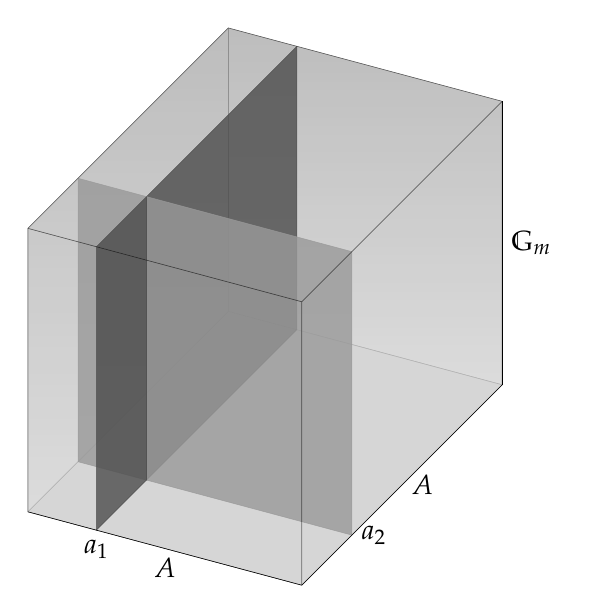
\begin{tikzpicture}[x  = {(-0.707cm,-0.707cm)},
                    y  = {(0.9659cm,-0.25882cm)},
                    z  = {(0cm,1cm)},
                    scale = 1.8,
                    color = {lightgray}]
% style of faces
\tikzset{facestyle/.style={fill=black!25,draw=black,very thin,line join=round,opacity=.4},slicestyle/.style={fill=black!25,draw=black,very thin,line join=round,opacity=.8}}
%\tikzset{facestyle/.style={fill=cyan,draw=blue,very thin,line join=round,opacity=.4},slicestyle/.style={fill=cyan,draw=blue,very thin,line join=round,opacity=.7}}
% face "back" 
\begin{scope}[canvas is zy plane at x=0]
  \path[facestyle,shade] (0,0) rectangle (2,2);
\end{scope}
% face  "left"
\begin{scope}[canvas is zx plane at y=0]
  \path[facestyle,shade] (0,0) rectangle (2,2);
\end{scope}
% face "down"
\begin{scope}[canvas is yx plane at z=0]
  \path[facestyle,color=lightgray] (0,0) rectangle (2,2);
\end{scope}
% face "red slice back"
\begin{scope}[canvas is zy plane at x=1.5]
  \path[slicestyle,color=black!50] (0,0) rectangle (2,0.5);
\end{scope}
% face "green slice back"
\begin{scope}[canvas is zx plane at y=0.5]
  \path[slicestyle,color=black] (0,0) rectangle (2,1.5);
\end{scope}
% face "red slice front"
\begin{scope}[canvas is zy plane at x=1.5]
  \path[slicestyle,color=black!50] (0,0.5) rectangle (2,2);
\end{scope}
% face "green slice front"
\begin{scope}[canvas is zx plane at y=0.5]
  \path[slicestyle,color=black] (0,1.5) rectangle (2,2);
\end{scope}
% face "front"
\begin{scope}[canvas is zy plane at x=2]
  \path[facestyle] (0,0) rectangle (2,2);
\end{scope}
% face  "right"
\begin{scope}[canvas is zx plane at y=2]
  \path[facestyle] (0,0) rectangle (2,2);
\end{scope}
% face "up" 
\begin{scope}[canvas is yx plane at z=2]
  \path[facestyle] (0,0) rectangle (2,2);
\end{scope}
% labels
\draw[very thin,black,line join=round]
     (2,0,0) -- node [below,black] {$A$} (2,2,0);
\draw[very thin,black,line join=round]
     (2,2,0) -- node [right,black] {$A$} (0,2,0);
\draw[very thin,black,line join=round]
     (0,2,0) -- node [right,black] {$\Gm$} (0,2,2);
\draw[very thin,black,line join=round]
     (2,0.5,0) -- node [below,black] {$a_1$} (2,0.5,0);
\draw[very thin,black,line join=round]
     (1.5,2,0) -- node [right,black] {$a_2$} (1.5,2,0);
\end{tikzpicture}
\hspace{0.5em}
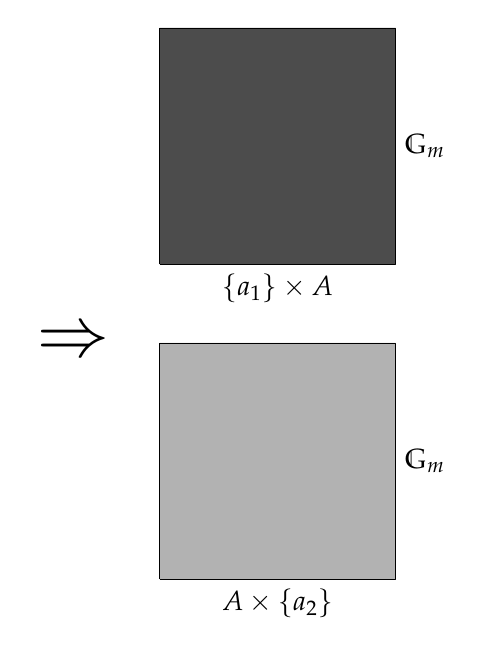
\begin{tikzpicture}
    \draw[very thin,black,line join=round,fill=black!30]
        (0,1) -- node [below,black] {$A \times \{a_2\}$} (3,1) -- node[right,black] {$\Gm$} (3,4) -- (0,4) -- (0,1);
    \draw[very thin,black,line join=round,fill=black!70]
        (0,5) -- node [below,black] {$\{a_1\} \times A$} (3,5) -- node[right,black] {$\Gm$} (3,8) -- (0,8) -- (0,5);
    \node[anchor=east] at (-0.5,4) {\Huge $\Rightarrow$};
\end{tikzpicture}
\end{center}
\caption{Extensions contained in a biextension.}
\end{figure}
There is a canonical piece of gluing data on this biextension, in the form of an isomorphism of pullback bundles
\begin{align*}
e_{p^j}\co (p^j \times 1)^* \L|_{A[p^j] \times A[p^j]} & \cong (1 \times p^j)^* \L|_{A[p^j] \times A[p^j]}, \\
(\ell, x, y) & \mapsto \left(\ell \cdot \prod_{k=1}^{p^j-1} \frac{s(x, [k]x, y)}{s(x, [k]y, y)} \right).
\end{align*}
This function $e_{p^j}$ is called the \textit{($p^j${\th}) Weil pairing}.
\end{definition}\todo{Can you prove some parts of this more carefully?}

\begin{remark}
In the case that $A$ is an elliptic curve, this agrees with the usual definition of its ``Weil pairing''. % In the case of an elliptic curve, this lines up with more traditional definitions --- for instance, using the isogeny $n: C \to C$.  In the case of a \emph{complex} elliptic curve $\C / (1, \tau)$, this degenerates further to the assignment \[\left( \frac{a}{n}, \frac{b}{n} \tau \right) \mapsto \exp\left(-2\pi i \frac{ab}{n}\right).\]
\end{remark}

\begin{lemma}\citeme{AS, I guess}
The Weil pairings assemble into a total Weil pairing on the $p$--divisible group associated to $A$.  Together, the total Weil pairing is alternating and biexponential\todo{What does biexponential mean?}. \qed
\end{lemma}

We can use the same formula in the setting of a cubical structure on a line bundle over a finite height formal group $\G$ to produce the desired map \[e_*\co C^3(\G; \Gm) \to \InternalHom{FormalGroups}(\G^{\wedge 2}, \Gm).\] \todo{How? What is $\ell$?} In fact, this is the right map:
\begin{lemma}[{\cite[Theorem 4.2, Corollary 4.4]{AndoStrickland}}]
The square commutes (up to sign):
\begin{center}
\begin{tikzcd}
\Spec E_0 BU[6, \infty) \arrow{r} \arrow{d}{\Pi_3} & \Spec E_0 K(\Z, 3) \arrow{d}{b_*} \\
C^3(\CP^\infty_E; \mathbb G_m) \arrow{r}{e} & \Weil(\CP^\infty_E).
\end{tikzcd}
\end{center}
\todo{You have not introduced the notation $\Weil$.
\end{lemma}
\begin{proof}[Proof sketch]
This is reasonably difficult.  The main points are to show that the restriction \[d_{p^j}\co BC_{p^j}^{\times 2} \xrightarrow{\beta \circ \mu} \OS{H\Z}{3} \to BU[6, \infty)\] can be expressed by the Weil pairing formula: \[d_{p^j} = \bigoplus_{k=1}^{p^j-1} \left((\L_1 - 1)(\L_1^{\otimes k} - 1)(\L_2 - 1) - (\L_1 - 1)(\L_2^{\otimes k} - 1)(\L_2 - 1)\right).\]  \todo{Where does $d_{p^j}$ appear in the diagram above?} After this is accomplished, what's left is to use naturality properties of the adjoint construction to compute the clockwise and counterclockwise composites.
\end{proof}

This fills out the diagram we are considering.  We now assemble just enough exactness results:

\begin{lemma}[{\cite[Lemma 7.2]{AndoStrickland}}]
The map $\delta\co C^2 \to C^3$ is injective for $\CP^\infty_E$ a finite height formal group.
\end{lemma}
\begin{proof}
Being finite height means that the multiplication-by-$p$ map of $\CP^\infty_E$ is fppf--surjective.  The kernel of $\delta$ consists of alternating, biexponential maps $(\CP^\infty_E)^{\times 2} \to \Gm$.  By restricting such a map $f$ to \[f \co \CP^\infty_E[p^j] \times \CP^\infty_E \to \Gm,\] we can calculate \[f(x, p^j y) = f(p^j x, y) = f(0, y) = 1.\]  But since $p^j$ is surjective on $\CP^\infty_E$, every point on the right-hand side can be so written, so at every left-hand stage the map is trivial.  Finally, $\CP^\infty_E = \colim_j \CP^\infty_E[p^j]$, so this filtration is exhaustive and we conclude that the kernel is trivial.
\end{proof}\todo{This doesn't sound like the proof that you and Hood gave in class?  Is that a different proof?}

\begin{lemma}[{\cite[Lemma 7.3]{AndoStrickland}}]
In fact, the following sequence is exact \[0 \to C^2(\CP^\infty_E; \Gm) \xrightarrow\delta C^3(\CP^\infty_E; \Gm) \to \Weil(\CP^\infty_E).\]
\end{lemma}
\begin{proof}
This is hard work.  Breen's idea is to show that picking a preimage under $\delta$ is the same as picking a trivialization of the underlying symmetric biextension of the cubical structure.  Then (following Mumford), one shows that the underlying symmetric biextension is trivial exactly if the Weil pairing is trivial.\todo{You could put in references here. AS gives them.}
\end{proof}

Finally, the top row falls quickly:

\begin{lemma}[{\cite[Lemma 7.5]{AndoStrickland}}]
\todo{Remark: This proof also shows that the $E$--theory of $\OS{kU}{8}$ fits into a sexseq.}
The top row of the main diagram is a short exact sequence of group schemes.
\end{lemma}
\begin{proof}
This is easiest proved by considering the sequence of homology Hopf algebras instead.  Since the integral homology of $BSU$ and the $E$--homology of $\OS{H\Z}{3}$ are both free and even, the Atiyah--Hirzebruch spectral sequence for $E_* BU[6, \infty)$ collapses.
\end{proof}

\begin{corollary}
The map \[\Pi_3\co \Spec E_0 BU[6, \infty) \to C^3(\CP^\infty_E; \Gm)\] is an isomorphism, and the map \[e_*\co C^3(\CP^\infty_E; \Gm) \to \InternalHom{FormalGroups}((\CP^\infty_E)^{\wedge 2}, \Gm)\] is a surjection.
\end{corollary}
\begin{proof}
This is a direct consequence of the $5$--lemma.
\end{proof}








% We begin with the fiber:

% \begin{lemma}[{\cite[Lemma 4.5]{AndoStrickland}}]\label{EasyCompatibilityWithdn}
% Write
% \begin{align*}
% d_n(\L_1, \L_2) & := \sum_{k=1}^{p^j-1} \left( (\L_1 - 1)(\L_1^k - 1)(\L_2 - 1) - (\L_1 - 1)(\L_2^k - 1)(\L_2 - 1)\right).
% \end{align*}
% There is a unique $\lambda \in \Z/n$ such that the following triangle commutes:
% \begin{center}
% \begin{tikzcd}
% (B\Z/p^j)^{\times 2} \arrow{d}{\lambda \beta \mu} \arrow{rd}{d_n(\L_1, \L_2)} \\
% K(\Z, 3) \arrow{r}{i} & BU[6, \infty).
% \end{tikzcd}
% \end{center}
% \end{lemma}
% \begin{proof}
% Forgetting down to $BU$ and working with just virtual bundles rather than lifts of virtual bundles to elements of $kU^6$, the definition of $d_n(\L_1, \L_2)$ gives
% \begin{align*}
% d_n(\L_1, \L_2) & = (\L_1 - 1)(\L_2^{p^j} - 1) - (\L_1^{p^k} - 1)(\L_2 - 1).
% \end{align*}
% Since we have restricted to $(B\Z/p^j)^{\times 2}$, $\L_1^{p^k} = 1$ and $\L_2^{p^k} = 1$, so this formula collapses and the composite map \[(B\Z/p^j)^{\times 2} \xrightarrow{d_n} BU[6, \infty) \xrightarrow{\pi_2} BSU \xrightarrow{\pi_2} BU\] is null.  We now study the lifting problem across the two maps:
% \begin{enumerate}
% \item[$\pi_1$:] Since the long composite is null, it follows that the shorter composite $\pi_2 \circ d_n$ factors through the fiber of $\pi_2$.  But, the fiber of $\pi_2$ is $S^1$, and there are no maps \[\{(B\Z/p^j)^{\times 2} \to S^1\} \cong H^1((B\Z/p^j)^{\times 2}; \Z) = 0.\]  It follows that $\pi_2 \circ d_n$ is itself null.
% \item[$\pi_2$:] Since $\pi_2 \circ d_n$ is null, $d_n$ must factor through the fiber of $\pi_2$, which is $K(\Z, 3)$.  With identical motives, one considers $H^3((B\Z/p^j)^{\times 2}; \Z)$, which is cyclic of order $n$ and generated by $\beta \circ \mu$. \qedhere
% \end{enumerate}
% \end{proof}

% \noindent This Lemma was missing a nontriviality statement, which turns out to be much harder:\todo{You could probably abbreviate the proof of this and include it.}

% \begin{theorem}[{\cite[Theorem 4.2, Section 5]{AndoStrickland}}]
% The value of $\lambda$ in \Cref{EasyCompatibilityWithdn} can be taken to be $\pm 1$. \qed
% \end{theorem}

% We now play one of our main cards: our willingness to work with cooperations means that we can pass from the hard task of checking facts about our formal schemes to the generally easier task of checking facts about their Cartier duals.  Because the formal schemes themselves are designed to have universal properties, their Cartier duals have points which are specified by these universal properties, and we win a considerable increase in tangibility.  In order to make full use of this, we record a mechanism of translation between these perspectives:


% These ideas power the following Lemma:

% \begin{proof}
% The target scheme $\Weil(\CP^\infty_E)$ is a subscheme of $\InternalHom{FormalGroups}((\CP^\infty_E)^{\times 2}, \Gm)$.  Since $\CP^\infty_E$ is finite height it satisfies $\CP^\infty_E = \colim_j \CP^\infty_E[p^j]$, which, coupled with the exponential adjunciton, reduces us to showing the agreement of the pair of composite maps \[\Spec E_0 BU[6, \infty) \times_{\S_E} \CP^\infty_E[p^j]^{\times 2} \to \Gm.\]  We will express these maps in terms of the adjoint map construction, starting with the clockwise composite.  The class $\beta \mu \in H\Z^3 BC_{p^j}^{\times 2}$ gives rise to an adjoint map \[\widehat{\beta \mu}\co \G_E[p^j]^{\times 2} \times (\OS{H\Z}{3})_E^\vee \to \Gm,\] which pulls back along $i\co \OS{H\Z}{3} \to \OS{kU}{6}$ to give \[(1 \times \Spec E_0 i) \circ \widehat{\beta \mu} = \widehat{i \beta \mu} = \widehat{d_n(\L_1, \L_2)}\] by the previous Theorem.

% We now try to calculate this adjoint, which will lead us to the counterclockwise composite.  First, the bundle $\bigotimes_{j=1}^3 (\L_j - 1) \in kU^6 (\CP^\infty)^{\times 3}$ gives rise to an adjoint map satisfying the following compatibility:
% \begin{center}
% \begin{tikzcd}
% (\CP^\infty_E)^{\times 3} \times \Spec E_0 BU[6, \infty) \arrow["\widehat{\bigotimes_{j=1}^3 (\L_j - 1)}"]{r} \arrow{d} & \Gm \\
% (\CP^\infty_E)^{\times 3} \times C^3(\CP^\infty_E; \Gm) \arrow{r} & (\CP^\infty_E)^{\times 3} \times \InternalHom{FormalSchemes}((\CP^\infty_E)^{\times 3}, \Gm) \arrow["\text{eval}"]{u}.
% \end{tikzcd}
% \end{center}
% The effect of postcomposing with the Weil pairing map can be viewed instead as precomposing the bottom-right corner with the






% \todo[inline]{This proof is unclear to the point of being broken.  How does the middle paragraph address the bottom-left arm of the square?}
% We will check compatibility on $\Weil_n(\CP^\infty_E)$ for arbitrary $n$, and so restrict from $i$ to $i \circ \lambda \beta \mu = d_n(\L_1, \L_2)$.
% % (Note: the sign can't bounce with $n$ because $\CP^\infty_E$ is $p$--divisible.)
% Since $\Weil_n(\CP^\infty_E)$ is a subscheme \[\Weil_n(\CP^\infty_E) \subseteq \InternalHom{FormalSchemes}(\CP^\infty_E[n]^{\times 2}, \Gm),\] we can push forward to checking equality here, i.e., of the two maps \[\Spec E_0 BU[6, \infty) \times_{\S_E} \CP^\infty_E[n]^{\times 2} \to \Gm.\]

% Writing $z = \prod_{i=1}^3 (1 - \L_i) \in kU^6 (\CP^\infty)^{\times 3}$, properties of the adjoint construction $\hat z$ show that it is given by the composite \[\hat z \co \Spec E_0 BU[6, \infty) \times_{\S_E} (\CP^\infty_E)^{\times 3} \to C^3(\CP^\infty_E; \Gm) \times_{\S_E} (\CP^\infty_E)^{\times 3} \xrightarrow{\operatorname{eval}} \Gm.\]  By specializing to $z = (1 - \L_1)(1 - \L_1^k)(1 - \L_2) \in kU^6 (\CP^\infty)^{\times 2}$, we see that $\hat z$ acts by\todo{Do I mean to be writing $k$--series here? I think I do.} \[\hat z \co (f, (g_1, g_2)) \mapsto f(g_1, [k](g_1), g_2),\] and continuing along these lines we see \[\widehat{d_n(\L_1, \L_2)} \co (f, (g_1, g_2)) \mapsto \prod_{k=1}^{n-1} \frac{f(g_1, [k](g_1), g_2)}{f(g_1, [k](g_2), g_2)} = e_n(f)(g_1, g_2).\]

% That described the bottom-left arm of the square.  The other way around the square is easier: take $w = \beta \circ \mu \in H^3(B\Z/p^j)^{\times 2}$ with adjoint $\hat w \co \CP^\infty_E[p^j]^{\times 2} \times K(\Z, 3)^E \to \Gm$.  Naturality shows $\hat w \circ \gamma^E = \widehat{\gamma_* w}$, and the theorem shows $\gamma_* w = \pm d_n(\L_1, \L_2)$, hence $\widehat{\gamma_* w} = (\pm d_n(\L_1, \L_2))\hat{}$, which is adjoint to $(e_n \Pi_3)^\pm$.
% \end{proof}

% \todo{There's a nice construction of the $\Pi_k$ maps in the AHS preprint where the ``$C_k$'' constructions are performed directly on the spectra, then applying $(-)_E$ carries those constructions to relevant constructions on group schemes, and finally Cartier duality gives the maps $\Pi_k$ of the sort described above.  This is superior to saying ``adjoint'', in my opinion, though it could be remarked that these are equivalent.}
% \todo{Consider including Lemma 6.2 and so on, the $BSU \to BU$ equivalents of the later statements you need.}

% % \begin{lemma}[{\cite[Lemma 6.2]{AndoStrickland}}]
% % The adjoint of the map $E_0 \CP^\infty \to E_0 BU$ induces a map $\Pi_1: BU^E \to C^1(\CP^\infty_E; \mathbb G_m)$ which is an isomorphism.  In fact, the Cartier duality isomorphism $(\CP^\infty)^E \cong \InternalHom{FormalGroups}(\CP^\infty_E, \mathbb G_m)$ fits into a commuting square
% % \begin{center}
% % \begin{tikzcd}
% % (\CP^\infty)^E \arrow{r} \arrow{d} & \InternalHom{FormalGroups}(\CP^\infty_E, \Gm) \arrow{d}{\begin{array}{c} \text{natural} \\ \text{inclusion} \end{array}} \\
% % BU^E \arrow{r}{\Pi_1} & C^1(\CP^\infty_E; \Gm).
% % \end{tikzcd}
% % \end{center}
% % \end{lemma}
% % \begin{proof}
% % \todo{Include this.}
% % \end{proof}

% % \begin{theorem}\label{BUBSUandC1C2Commute}
% % The following square commutes:
% % \begin{center}
% % \begin{tikzcd}
% % BU^E \arrow{d}{\Pi_1} \arrow{r} & BSU^E \arrow{d}{\Pi_2} \\
% % C^1(\CP^\infty_E; \Gm) \arrow{r}{\delta} & C^2(\CP^\infty_E; \Gm).
% % \end{tikzcd}
% % \end{center}
% % \end{theorem}
% % \begin{proof}
% % \citeme{Lemma 6.4 of AS}
% % This is a matter of expanding definitions and using \[(\L_1 - 1)(\L_2 - 1) = \mu^*(\L - 1) - \pi_1^*(\L - 1) - \pi_2(\L - 1).\]
% % \end{proof}

% % \begin{theorem}
% % The following is a map of short exact sequences:
% % \begin{center}
% % \begin{tikzcd}
% % 0 \arrow{r} & (\CP^\infty)^E \arrow{d} \arrow{r} & BU^E \arrow{r} \arrow{d} & BSU^E \arrow{r} \arrow{d} & 0 \\
% % 0 \arrow{r} & \InternalHom{FormalGroups}(\CP^\infty_E; \Gm) \arrow{r} & C^1(\CP^\infty; \Gm) \arrow{r} & C^2(\CP^\infty; \Gm) \arrow{r} & 0.
% % \end{tikzcd}
% % \end{center}
% % \end{theorem}
% % \begin{proof}
% % \citeme{Prop 6.5 of AS. They reference a superior alternate argument in the AHS preprint though\ldots}
% % \end{proof}








\section{Unstable additive cooperations for $kU$}

Write $H = H\F_p$.  Today we will study the effect of the map $\hat \Pi_3$ in ordinary homology.  Many parts of the proof we explored for $E$--theory break.  Topologically, the Serre spectral sequence for $H^* BU[6, \infty)$ is not even-concentrated and so is not forced to collapse.  Algebraically, because $\G_a$ is not $p$--divisible the behavior of the model exact sequence is also suspect.  Because the situation has fewer insulating good properties, we are forced to actually consider it carefully.  The upside, however, is that the standard group law on $\G_a$ is simple enough that we can compute the problem to death.

We begin with the topological half of our tasks.  The Serre spectral sequence \[E_2^{*, *} = H\F_p^* BSU \otimes H\F_p^* \OS{H\Z}{3} \Rightarrow H\F_p^* BU[6, \infty)\] is quite accessible, and we will recount the case of $p = 2$.  In this case, the spectral sequence has $E_2$--page \[E_2^{*, *} = H\F_2^* BSU \otimes H\F_2^* \OS{H\Z}{3} \cong \F_2[c_2, c_3, \ldots] \otimes \F_2\left[\Sq^I \iota_3 \middle| \begin{array}{c} I_j \ge 2I_{j+1}, \\ 2 I_1 - I_+ \end{array}\right].\] \todo{$2 I_1 - I_+$ doesn't look like a condition.  Also, what is $I_+$?  Somehow this should mean that you start with $\Sq^2$ not $\Sq^1$.}  Because the target is $6$--connective, we must have the transgressive differential $d_4 \iota_3 = c_2$, which via the Kudo transgression theorem spurs the much larger family of differentials \[d_{4+I_+} \Sq^I \iota_3 = \Sq^I c_2.\]  This necessitates understanding the action of the Steenrod operations on the cohomology of $BSU$, which is due to Wu\citeme{Wu formulas, maybe May's concise book}:\todo{Can these formulas be read off from the divisorial calculation?  Maybe not, since it's easy to read off the Milnor primitives but harder to see the Steenrod squares.} \[\Sq^{2^j} \cdots \Sq^4 \Sq^2 c_2 = c_{1 + 2^j}.\]  Accounting for the squares of classes left behind, this culminates in the following calculation:\todo{This spectral sequence can be drawn in using Hood's package.}

\begin{theorem}\label{HF2BU6Calculation}
There is an isomorphism \[H\F_2^* BU[6, \infty) \cong \frac{H\F_2^* BU}{(c_j \mid j \ne 2^k + 1, j \ge 3)} \otimes F_2[\iota_3^2, (\Sq^2 \iota_3)^2, \ldots]. \qed\]
\end{theorem}

\begin{theorem}\citeme{Stong, Singer}
More generally, there is an isomorphism \[H\F_2^* \OS{kU}{2k} \cong \frac{H\F_2^* BU}{(c_j \mid \sigma_2(j - 1) < k - 1)} \otimes \operatorname{Op}[\Sq^3 \iota_{2k-1}],\] where $\sigma_2$ is the dyadic digital sum and ``$\operatorname{Op}$'' denotes the subalgebra of $H\F_2^* \OS{H\Z}{2k-1}$ generated by the indicated class.
\end{theorem}
\begin{proof}[Remarks on proof]
Stong specialized to $p = 2$ and carefully applied the Serre spectral sequence to the fibrations \[\OS{kU}{2(k+1)} \to \OS{kU}{2k} \to \OS{H\Z}{2k}.\]  Singer worked at an arbitrary prime and used the Eilenberg--Moore spectral sequence for the fibrations \[\OS{H\Z}{2k-1} \to \OS{kU}{2(k+1)} \to \OS{kU}{2k}.\]  Both used considerable knowledge of the interaction of these spectral sequences with the Steenrod algebra.
\end{proof}

\begin{remark}
These methods and results generalize directly to odd primes.  The necessary modifications come from understanding the unstable mod--$p$ Steenrod algebra, using the analogues of Wu's formulas due to Shay\citeme{Wu formulas, Shay's extension in \textit{mod--$p$ Wu formulas for the Steenrod algebra and the Dyer--Lashof algebra}}, and employing Singer's Eilenberg--Moore calculation.  Again, $H\F_p^* BU[6, \infty)$ is presented as a quotient by $H\F_p^* BU$ by certain Chern classes satisfying a $p$--adic sum condition, tensored up with the subalgebra of $H\F_p^* \OS{H\Z}{3}$ generated by a certain element.
\end{remark}

\begin{remark}
We can already see from \Cref{HF2BU6Calculation} that our map of short exact sequences in \Cref{ChromaticKUCoopnsSection} does not have a full analogue in the setting of additive homology.  By considering the edge homomorphism in the Serre spectral sequence, we see that \[\Spec HP_0 BSU \to \Spec HP_0 BU[6, \infty)\] is not a monomorphism.
\end{remark}





Now, we turn to the algebra.  The main idea, as already used in \Cref{CalculationOfLTTangentSpace}\todo{Is this really the best example to reference?}, is to first perform a tangent space calculation \[T_0 C^k(\G_a; \Gm) \cong C^k(\G_a; \G_a),\] then study the behavior of the different tangent directions to determine the full object $C^k(\G_a; \Gm)$.  As a warm-up, we will first consider the case $k = 2$:
\begin{corollary}[{cf.\ \Cref{CohomologyOfGa}}]
The unique symmetric $2$--cocycle of homogeneous degree $n$ has the form \[c_n(x, y) = \begin{cases} (x + y)^n - x^n - y^n & \text{if $n \ne p^j$}, \\ \frac{1}{p} \left( (x + y)^n - x^n - y^n \right) & \text{if $n = p^j$}. \end{cases} \qed\]
\end{corollary}

Our goal, then, is to select such a $2$--cocycle $f$ and study the minimal conditions needed on a symbol $a$ to produce a multiplicative $2$--cocycle of the form $1 + af + \cdots$.  Since $c_n = \frac{1}{d_n} \delta(x^n)$ \todo{The notation is a little odd, since you're conflating $x^n$ with the function $x \mapsto x^n$.} is itself produced by an additive formula, life would be easiest if we had access to an exponential, so that we could build \[\text{``$ \delta \exp(a_n x^n)^{1/d_n} = \exp(\delta a_n x^n / d_n) = \exp(a_n c_n). $''}\]  However, the existence of an exponential series is equivalent to requiring that $a_n$ have all fractions, which turns out not to be minimal.  In fact, \emph{no} conditions on $a_n$ are required \emph{at all}, if we tweak the definition of an exponential series:

\begin{definition}\todo{Where does this come from? I've never learned a universal property for it. That bothers me. It must have something to do with $p$--typification.}
The \textit{Artin--Hasse exponential} is the power series \[E_p(t) = \exp\left( \sum_{j=0}^\infty \frac{t^{p^j}}{p^j} \right) \in \Z_{(p)}\ps{t}.\]
\end{definition}

This series has excellent properties, mimicking those of $\exp(t)$ as closely as possible while keeping coefficients in $\Z_{(p)}$ rather than in $\Q$.  Writing $\delta\co C^1 \to C^2$ and \[d_n = \begin{cases} 1 & \text{if $n = p^j$}, \\ 0 & \text{otherwise}, \end{cases}\] we set \[g_n(x, y) := \delta E_p(a_n x^n)^{1/p^{d_n}} = \exp\left( \sum_{j=0}^\infty \frac{a_n^{p^j} \delta x^{np^j}}{p^{j + d_n}} \right) = \exp\left( \sum_{j=0}^\infty \frac{a_n^{p^j} c_{np^j}(x, y)}{p^j} \right).\]  This gives a point in $C^2(\G_a; \Gm)(\Z_{(p)}[a_n])$, and exhaustion of the tangent space\todo{Granting that this exhausts the tangent space, how do we recover the global scheme?  Even if we had an inverse function theorem (like Thm.~2.1.4), I would only expect that to be at most a local isomorphism -- unless these are all really formal schemes masquerading as ordinary schemes?} proves the following Lemma:

\begin{lemma}[{\cite[Proposition 3.9]{AHSTheoremOfTheCube}}]
The map \[\Spec \Z_{(p)}[a_n \mid n \ge 2] \xrightarrow{\prod_{n \ge 2} g_2} C^2(\G_a; \Gm) \times \Spec \Z_{(p)}\] is an isomorphism. \qed
\end{lemma}

The case $k = 3$ is similar, with one important new wrinkle.  Over an $\F_2$--algebra there is an equality $c_n^2 = c_{2n}$.  However, this relation does not generalize to trivariate $2$--cocycles:
\begin{align*}
\frac{1}{2} \delta (c_6) & = x^2 y^2 z^2 + x^4 y z + x y^4 z + x y z^4, &
\left(\frac{1}{2} \delta c_3\right)^2 & = x^2 y^2 z^2.
\end{align*}
This pattern is generic and exhaustive for $\F_p$--algebras:
\begin{lemma}[{\cite[Proposition 3.20, Proposition A.12]{AHSTheoremOfTheCube}}]
The $p$--primary residue of the scheme of trivariate symmetric $2$--cocycles is presented by \[\Spec \F_p[a_d \mid d \ge 3] \times \Spec \F_p[b_d \mid d = p^j(1 + p^k)] \xrightarrow{\cong} C^3(\G_a; \G_a) \times \Spec \F_p. \qed\]
\end{lemma}

\noindent Similar juggling of the Artin--Hasse exponential yields the following multiplicative classification:
\begin{theorem}[{\cite[Proposition 3.28]{AHSTheoremOfTheCube}}]
There is an isomorphism \[\Spec \Z_{(p)}[a_d \mid d \ge 3, d \ne 1 + p^t] \times \Spec \Gamma[b_{1 + p^t}] \xrightarrow{} C^3(\G_a; \Gm) \times \Spec \Z_{(p)}.\]
\end{theorem}
\begin{proof}[Proof sketch]
The main claim is that the Artin--Hasse exponential trick used in the case $k = 2$ works here as well, provided $d \ne 1 + p^t$ so that taking an appropriate $p${\th} root works out.  They then show that the remaining exceptional cases extend to multiplicative cocycles only when the $p${\th} power of the leading coefficient vanishes.  Finally, a rational calculation shows how to bind these truncated generators together into a divided power algebra.
\end{proof}

In our pursuit of the map of exact sequences of \Cref{ChromaticKUCoopnsSection}, we are missing one piece: a link from topology to the scheme of Weil pairings, $\Weil(\G_a)$.  The object ``$\Spec HP_0 \OS{H\Z}{3}$'' is insuitable because it doesn't exist --- the homology algebra $HP_0 \OS{H\Z}{3}$ is not even--concentrated.  However, analyzing the edge homomorphism from our governing Serre spectral sequence shows that the map \[HP^0 BU[6, \infty) \to HP^0 \OS{H\Z}{3}\] factors through the subalgebra $A$ generated by the \emph{squares} of the polynomial generators.  Accordingly, we aim to place $\Spec A^*$ in the top-right corner of our map of 

\begin{lemma}[{\cite[Lemma 3.36, Proposition 4.13, Lemma 4.11]{AHSTheoremOfTheCube}}]
The scheme $\Spec A^*$ models $\Weil(\G_a)$ by an isomorphism $\lambda$ commuting with $e \circ \hat \Pi_3$.
\end{lemma}
\begin{proof}[Proof sketch]
The $\F_p$--scheme $\Weil(\G_a)$ is simple to describe:
\begin{center}
\begin{tikzcd}[row sep=1em]
(a_{mn})_{m, n} \arrow[|->]{r} & \prod_{m < n} \operatorname{texp}\left(a_{mn}(x^{p^m} y^{p^n} - x^{p^n} y^{p^m})\right) \\
\Spec \F_p[a_{mn} \mid m < n] / (a_{mn}^p) \arrow{r}{\cong} & \Weil(\G_a),
\end{tikzcd}
\end{center}
where $\operatorname{texp}(t) = \sum_{j=0}^{p-1} t^j / j!$ is the truncated exponential series.  It is easy to check that this ring of functions agrees with $A^*$, and it requires hard work (although not much creativity) to check the remainder of the statement: that $e \circ \hat \Pi_3$ factors through $\Spec A^*$ and that the factorization is an isomorphism.
\end{proof}

We have now finally assembled our map of right-exact sequences:\todo{It's maybe not obvious to a reader why this sequence is exact in the middle, although you have secretly proven this in the mess above.}
\begin{center}
\begin{tikzcd}
\Spec HP_0 BSU \arrow{r} \arrow["\hat \Pi_2", "\cong"']{d} & \Spec HP_0 BU[6, \infty) \arrow{r} \arrow["\hat \Pi_3"]{d} & \Spec A^* \arrow{r} \arrow["\lambda", "\cong"']{d} & 0 \\
C^2(\G_a; \Gm) \arrow{r}{\delta} & C^3(\G_a; \Gm) \arrow{r}{e} & \Weil(\G_a) \arrow{r} & 0.
\end{tikzcd}
\end{center}
Our calculations now pay off:
\begin{corollary}
The map $\hat \Pi_3$ is an isomorphism: \[\hat \Pi_3\co \Spec HP_0 BU[6, \infty) \xrightarrow{\cong} C^3(\G_a; \Gm).\]
\end{corollary}
\begin{proof}[Proof sketch]
The main point is that we don't actually have to compute much about the middle map.  Because the squares commute and the sequences are exact as indicated, we at least learn that $\hat \Pi_3$ is an epimorphism after base-change to $\Spec \Q$ and $\Spec \F_p$ for each prime $p$.  But, since both source and target are affine schemes of graded finite type with equal Poincar\'e series in each case, our epimorphism is an isomorphism.
\end{proof}

\begin{corollary}[{\cite[Theorem 2.31]{AHSTheoremOfTheCube}}]\label{Pi3ForCplxOrientableE}
The map $\hat \Pi_3$ is an isomorphism for any complex-orientable $E$.\todo{Jay asked in class for a summary of exactly what exactness statements are true for a general $E$ (especially relative to the extreme case of $E$--theory, where everything is exact and pleasant).}
\end{corollary}
\begin{proof}[Proof sketch]
This follows much along the lines of \Cref{HopfRingForEBP}.  We check that the statement holds for $E = MUP$ using a tangent space argument, and then an Atiyah--Hirzebruch argument gives the statement for any complex-oriented $E$.
\end{proof}

\begin{remark}
Our analysis in \Cref{LEFTCooperations} gives us full access to the Hopf ring structure of the \emph{nonconnective} cooperations $H\F_p{}_* \OS{KU}{2*}$.  Using a variety of techniques, Morton and Strickland calculated the Hopf ring structure of $H\F_2{}_* \OS{K}{2*}$ where $K$ ranges among the nonconnective objects $KO$, $KU$, $KSp$, and the less common ``$KT$'', which is self--conjugated $K$--theory~\cite{Morton,MortonStrickland,StricklandBottPeriodicity}.\todo{This could be expanded some, as not all these references are relevant to what's written.}
\end{remark}










\section{Covariance, $\Theta$--structures on Thom sheaves}

Today we will (despite appearances) mostly leave the algebraic geometry alone, instead attending to two lingering topological concerns.  First, over the past few lectures we have been concerned with the homology schemes $\Spec E_0 \OS{kU}{2*}$.  We were originally motivated by a sequence of cohomological isomorphisms
\begin{align*}
(BU \times \Z)_E & \cong \Sym^0_{\Div \CP^\infty_E} \Div_0 \CP^\infty_E =: C_0 \CP^\infty_E, \\
BU_E & \cong \Sym^1_{\Div \CP^\infty_E} \Div_0 \CP^\infty_E =: C_1 \CP^\infty_E, \\
BSU_E & \cong \Sym^2_{\Div \CP^\infty_E} \Div_0 \CP^\infty_E =: C_2 \CP^\infty_E,
\end{align*}
along with identifications
\begin{align*}
BU \times \Z & \simeq \OS{kU}{2 \cdot 0}, &
BU & \simeq \OS{kU}{2 \cdot 1}, &
BSU & \simeq \OS{kU}{2 \cdot 2}.
\end{align*}
Our analysis of Cartier duality in \Cref{TopologicalCartierDuality} gave us isomorphisms like \[\Spec E_0 BSU \cong \InternalHom{GroupSchemes}(BSU_E, \Gm) \cong \InternalHom{FormalGroups}(C_2 \CP^\infty_E, \G_m).\] Following the universal property of this particular symmetric square, we were led to consider the scheme of symmetric bivariate functions on $\CP^\infty_E$ satisfying a $2$--cocycle condition.  Our next move was to show that $\Spec E_0 BU[6, \infty)$ was modeled by a similar scheme of \emph{trivariate} functions --- but we proved this directly, while avoiding the ``predual'' cohomological statement \[BU[6, \infty)_E \cong C_3 \CP^\infty_E := \Sym^3_{\Div \CP^\infty_E} \Div_0 \CP^\infty_E.\]  This is because the homological statement is the low-hanging fruit: it is easy to demonstrate that the scheme of such functions exists as a closed subscheme of all functions.  It is considerably harder to show that a symmetric cube exists at all.

\begin{lemma}\label{CkGaGmAreFVars}\citeme{4.41 in the AHS preprint}
$DC^k(\G_a; \Gm)$ are all formal varieties for $k \le 3$.
\end{lemma}
\begin{proof}
We know that $\sheaf O C^k(\G_a; \Gm)$ are all free $\Z$--modules of graded finite rank in the range $k \le 3$\todo{Cite this from a couple lectures ago.}, so we may write \[\sheaf O(D C^k(\G_a; \Gm)) \cong (\sheaf O C^k(\G_a; \Gm))^*.\]  We will show that this later Hopf algebra $\sheaf O(C^k(\G_a; \Gm))^*$ is a power series ring, specializing for the moment to the case $k = 2$.  It will suffice to show that it is a power series ring modulo $p$ for every prime $p$.  Such graded connected finite-type Hopf algebras over $\F_p$ were classified by Borel (and exposited by Milnor--Moore~\cite[Theorem 7.11]{MilnorMoore}) as either polynomial or truncated polynomial.  These two cases are distinguished by the Frobenius operation: the Frobenius on a polynomial ring is injective, whereas the Frobenius on a truncated polynomial ring is not.  It is therefore equivalent to show that the \emph{Verschiebung} on the original ring $\sheaf O(C^2(\G_a; \Gm)) \otimes \F_p$ is \emph{surjective}.  Recalling that $c_n^p = c_{np}$ at the level of bivariate $2$--cocycles, we compute \[p^* a_n = a_{np}^p,\] and since $F a_{np} = a_{np}^p$ and $FV = p^*$, we learn \[V(a_{np}) = a_n.\] \todo{You should remind us that $c_n$ , $a_n$ were the things defined in the last lecture.}

Essentially the same proof handles the cases $k = 1$ and $k = 0$.  The case $k = 3$ requires a small modification, to cope with the two classes of trivariate $2$--cocycles.  On the polynomial tensor factor of $\sheaf O(C^3(\G_a; \Gm))$ we can reuse the same Verschiebung argument to see that its dual Hopf algebra is polynomial.  The dual of the divided power tensor factor is immediately a primitively generated polynomial algebra, without any further argument \todo{I'm confused about this statement.  Why doesn't something similar hold for the polynomial factor, given that it is true?}.
\end{proof}

\begin{theorem}
The scheme $C_3 \CP^\infty_E$ exists, and it is modeled by $BU[6, \infty)_E$.
\end{theorem}
\begin{proof}[Proof sketch]
\todo{This regurgitated proof is pretty broken.}
\citeme{Prop 3.3 in AHS preprint}
Let $\G$ be an arbitrary formal group.  Note first that if $C^3(\G; \Gm)$ is coalgebraic, then $C_3 \G$ exists and is its Cartier dual: the diagram presenting $\sheaf O(C^3(\G; \Gm))$ as a reflexive coequalizer of free Hopf algebras is also the diagram meant to present $C_3 \G$ as a coalgebraic formal scheme.  So, if the coequalizing Hopf algebra has a good basis, it will follow from \Cref{CoalgebraicColimitsExist} that the resulting diagram is a colimit diagram in formal schemes, with $C_3 \G$ sitting at the cone point.  It will additionally follow from there that the isomorphism from \Cref{Pi3ForCplxOrientableE} \[\Spec E_0 BU[6, \infty) \xrightarrow{\cong} C^3(\CP^\infty_E; \Gm)\] will re-dualize to an isomorphism \[BU[6, \infty)_E \xleftarrow{\cong} C_3 \CP^\infty_E.\]

\citeme{Prop 3.4 in the AHS preprint}
\todo{Here we are again, making grading arguments. We've been bad about this earlier in the paper too.}
So, we reduce to checking that $\sheaf O(C^3(\G; \Gm))$ admits a good basis.  By a base change argument, it suffices to take $\G$ to be the universal formal group over the Lazard ring.  Noting that $\sheaf O(C^3(\G; \Gm))$ must be of graded finite type, we will work to show that it is free on a basis we have good control over.

Specializing from $\G$ over $\moduli{fgl}$ to $\G_a$ over $\Spec \Z$, we know from \Cref{CkGaGmAreFVars} that $\sheaf O(C^3(\G_a; \Gm))$ is a free abelian group, and we know from \Cref{LazardsTheorem} that $\sheaf O(\moduli{fgl})$ is as well.  By picking a $\Z$--basis $\Z\{\beta_j\}_j$ of $\sheaf O C^3(\G_a; \Gm)$, we can choose a map of $\sheaf O(\moduli{fgl})$--modules lifting it
\begin{center}
\begin{tikzcd}
\sheaf O(\moduli{fgl})\{\tilde \beta_j\}_j \arrow["\alpha"]{r} \arrow{d} & \sheaf O C^3(\G; \Gm) \arrow{d} \\
\Z\{\beta_j\}_j \arrow["\cong"]{r} & \sheaf O C^3(\G_a; \Gm).
\end{tikzcd}
\end{center}
By induction on degree, one sees that $\alpha$ is surjective, and since the source is a free abelian group we need only check that the source and target have the same Poincar\'e series to conclude that $\alpha$ is an isomorphism.

We proceed to test this rationally: over $\Spec \Q$ we can use the logarithm to construct an isomorphism \[\Spec \Q \times (\moduli{fgl} \times C^k(\G; \Gm)) \to \Spec \Q \times (\moduli{fgl} \times C^k(\G_a; \Gm)),\] hence the Poincar\'e series agree, so $\alpha \otimes \Q$ and $\alpha$ are both isomorphisms.  Having established freenss, our other goal was to show that $M$ has a sequence of good subcoalgebras.  These come by considering the subcoalgebras, indexed on an integer $d$, spanned by the basis vectors of degree at most $d$.
\end{proof}

Our second task today is to address the gap between $\OS{kU}{2k}$ and its Thom spectrum $T(\OS{kU}{2k})$.  After all, our motivation for all of this algebraic geometry is to give a description to the set \[(\Spec E_0 MU[6, \infty))(E_0),\] but what we have done so far is describe the scheme $\Spec E_0 BU[6, \infty)$.  Since these two spectra are related by a Thom construction, we should be able to deduce the description that we want by thinking about Thom sheaves.  We now straighten this out.  The place to start is with a construction:

\begin{lemma}
For $\xi\co G \to BGL_1 \S$ a group map, the Thom spectrum $T\xi$ is a $(\Susp^\infty_+ G)$--cotorsor.
\end{lemma}
\begin{proof}[Proof sketch]
The Thom isomorphism $T\xi \sm T\xi \simeq T\xi \sm \Susp^\infty_+ G$ composes with the unit map $\S \to T\xi$ \todo{Which factor are we composing into? Does it matter?} to give the \textit{Thom diagonal} \[T\xi \to T\xi \sm \Susp^\infty_+ G. \qedhere\]
\end{proof}

\begin{corollary}
In addition to our interpretation of $\ThomSheaf{\xi}$ as a $\Gm$--torsor over $G_E$, $\ThomSheaf{\xi}^{-1}$ is furthermore a $(G_E \times \Gm)$--torsor over $S_E$\todo{$S_E$ vs.\ $\S_E$, and how does this follow?}. \qed
\end{corollary}

We expand this idea out in our situation.  A morphism $MU[6, \infty) \to E$ produces a trivialization of $\ThomSheaf{\bigotimes_{j=1}^3 (\L_j - 1)}$ over $(\CP^\infty_E)^{\times 3}$, and the associated trivializing section is symmetric and rigid\citeme{Lemma 2.49 of AHS}.  This prompts us to make the following definition:

\begin{definition}
We write $C^k(\G; \sheaf L)$ for the functor of trivializing sections of $\Theta^k \sheaf L$ over $\G^{\times k}$ which are symmetric and rigid.  This construction has some nice properties:
\begin{itemize}
\item Note that taking the trivial sheaf $\sheaf L = \sheaf O_{\G}$ recovers the scheme $C^k(\G; \Gm)$ of $\Gm$--valued such functions from before.
\item By consequence, if $\sheaf L$ is \emph{trivializable} then this functor is an affine scheme.
\item Affine or not, there is a pairing map \[C^k(\G; \sheaf L) \times C^k(\G; \sheaf H) \to C^k(\G; \sheaf L \otimes \sheaf H).\]  In particular, this recovers the group structure on $C^k(\G; \Gm)$ and it makes $C^k(\G; \sheaf L)$ into a $C^k(\G; \Gm)$--torsor.
\end{itemize}
\end{definition}

\noindent Thus, we have constructed a map \[\phi\co \Spec E_0 MU[6, \infty) \to C^3(\CP^\infty_E; \sheaf I(0)).\] The following Lemma is a matter of fully expanding definitions:

\begin{lemma}[{\cite[Theorem 2.50]{AHSTheoremOfTheCube}}]
The map \[\Spec E_0 MU[6, \infty) \to C^3(\CP^\infty_E; \sheaf I(0))\] is an isomorphism.
\end{lemma}
\begin{proof}[Proof sketch]
\todo{You shouldn't call this anything more than a ``proof sketch'' unless you expand out the reasoning for why this square commutes.}
This map is equivariant, in the sense that the following square commutes:
\begin{center}
\begin{tikzcd}
\Spec E_0 MU[6, \infty) \times \Spec E_0 BU[6, \infty) \arrow{r} \arrow{d}{\phi \times \text{\ref{Pi3ForCplxOrientableE}}} & \Spec E_0 MU[6, \infty) \arrow{d}{\phi} \\
C^3(\CP^\infty_E; \sheaf I(0)) \times C^3(\CP^\infty_E; \Gm) \arrow{r} & C^3(\CP^\infty_E; \sheaf I(0)).
\end{tikzcd}
\end{center}
Any equivariant map of torsors is automatically an isomorphism.
\end{proof}

\noindent This, finally, gives us access to the analogue of \Cref{BUZTriumvirate}, \Cref{BUTriumvirate}, and \Cref{BSUTriumvirate}:

\begin{corollary}\label{BU6Triumvirate}
Take $E$ to be \emph{complex--orientable}.  The functor $C^3(\CP^\infty_E; \sheaf I(0))$ defined by
\begin{align*}
\CatOf{AffineSchemes}_{/\Spec E_0} & \to \CatOf{Sets}, \\
(\Spec T \xrightarrow{u} \Spec E_0) & \mapsto \left\{ \begin{array}{c} \text{symmetric, rigid trivializations} \\ \text{of $u^* \Theta^3 \ThomSheaf{\L}$ over $u^* (\CP^\infty_E)^{\times 3}$} \end{array} \right\}
\end{align*}
is isomorphic to the affine scheme $\Spec E_0 MU[6, \infty)$.  Moreover, the $E_0$--points of this scheme biject with ring spectrum maps $MU[6, \infty) \to E$. \qed
\end{corollary}

\todo{This is a leftover todo from the following section.  We accomplish all of this here, but I haven't looked at the references tacked on at the end of this to see if they say anything I've missed.  --- --- --- --- --- I want to sketch the reduction for even-periodic elliptic cohomology theories to the case of $MUP$, then from there to $HkP$ for the prime fields $K$, then from there to questions about additive cocycles.  We certainly don't need to recall any of these calculations, but I think it's a nice example of the philosophy that the additive formal group is such a knotted point of $\moduli{fg}$ that it suffices to check something there to learn it for the rest of the stack.  This survives in the published form of AHS, but it's stated pretty clearly as Prop 3.4 in the unpublished verison.  See also 5.12 of the unpublished version.}

% \begin{remark}\todo[color=red]{Actually work this out.}
% It should be possible to give an example of a complex-oriented theory which receives an $MSU$ orientation which \emph{does not} factor the complex orientation but \emph{does} (\emph{must}, really) factor the unit?  Even if one can find an example of this, I think it will be somewhat artificial: the sequence of group schemes \[0 \to BSU_E \to BU_E \to BU(1)_E \to 0\] is short exact, \emph{and} it has a splitting on the level of formal schemes.  The splitting is what gives you the isomorphism on points $BSU_E(T) \times BU(1)_E(T) \cong BU_E(T)$.  On the other hand, because the splitting \emph{isn't} a map of formal groups, it doesn't survive to the Cartier dual short exact sequence \[0 \from BSU^E \from BU^E \from BU(1)^E \from 0,\] so this will come down to exhibiting a test ring $T = E_*$ for which $BU^E(T) \to BSU^E(T)$, despite being induced by an fppf-surjective map of sheaves, is not surjective on sections over $T$.  Of course, this comes down concretely to solving for a preimage under the map \[1 - g(x) \mapsto \frac{1 - g(x +_{\G} y)}{(1 - g(x))(1 - g(y))},\] which is more plodding but might offer insight into what sort of ring (and thus orientation) you're looking for.
% \end{remark}












\section{Modular forms from $MU[6, \infty)$--manifolds}

Our goal today is to actually leverage the arithmetic geometry in \Cref{Theta3IsTrivial}, rather than just using the body of results about $\theta$--functions as inspiration.  In order to do this, we need to place ourselves in a situation where algebraic topology is directly linked to abelian varieties.

\begin{definition}\label{DefnEllipticSpectrum}
An \textit{elliptic spectrum} consists of a even--periodic ring spectrum $E$, a (generalized) elliptic curve $C$ over $\Spec E_0$, and a fixed isomorphism \[\phi\co C^\wedge_0 \xrightarrow{\cong} \CP^\infty_E.\]  A map among such spectra consists of a map of ring spectra $f\co E \to E'$ together with a specified isomorphism of elliptic curves $\psi\co f^* C \to C'$.
\end{definition}

\begin{remark}
We have chosen to consider \emph{isomorphisms} of elliptic curve rather than general homomorphisms because this is what algebraic topology suggests that we do.  After all, the mixed cooperations of complex-oriented ring spectra are modeled by the isomorphisms of the associated formal groups.  In the next Case Study, we will develop a theory (with an attendant notion of a ``context'') which incorporates isogenies of elliptic curves in addition to isomorphisms.
\end{remark}

Coupling \Cref{DefnEllipticSpectrum} to \Cref{BU6Triumvirate} and \Cref{Theta3IsTrivial}, we learn the following result:
\begin{corollary}\label{EllipticSpectraAreOriented}
An elliptic spectrum $(E, C, \phi)$ receives a canonical map of ring spectra \[MU[6, \infty) \to E.\]  This map is natural in choice of elliptic spectrum: if $(E, C, \phi) \to (E', C', \phi')$ is a map of elliptic spectra, then the triangle
\begin{center}
\begin{tikzcd}
& MU[6, \infty) \arrow{ld} \arrow{rd} \\
E \arrow{rr} & & E'
\end{tikzcd}
\end{center}
commutes. \qed
\end{corollary}

\begin{example}
Our basic example of an elliptic curve was $E_\Lambda = \C / \Lambda$, with $\Lambda$ a complex lattice.  The projection $\C \to \C / \Lambda$ has a local inverse which defines an isomorphism of formal groups \[\phi\co (E_\Lambda)^\wedge_0 \xrightarrow{\cong} \G_a \otimes \C.\]  Accordingly, we define an elliptic spectrum $HE_\Lambda P$ whose underlying ring spectrum is $H\C$ and whose associated elliptic curve and isomorphism are $E_\Lambda$ and $\phi$.  This spectrum receives a natural map \[MU[6, \infty) \to HE_\Lambda P,\] which to a bordism class $M \in MU[6, \infty)_{2n}$ assigns an element $\Phi_\Lambda(M) \cdot u_\Lambda^n \in HE_\Lambda P_{2n}$ \todo{What is $u_\Lambda^n$?  How is it normalized?} for some $\Phi_\Lambda(M) \in \C$.
\end{example}

\begin{example}
The naturality of the $MU[6, \infty)$--orientation moves us to consider more than one elliptic spectrum at a time.  If $\Lambda'$ is another lattice with $\Lambda' = \lambda \cdot \Lambda$, then the multiplication map $\lambda\co \C \to \C$ descends to an isomorphism $E_\Lambda \to E_{\Lambda'}$ and hence a map of elliptic spectra $HE_{\Lambda'}P \to HE_\Lambda P$ acting by $u_{\Lambda'} \mapsto \lambda u_\Lambda$.  The commuting triangle in \Cref{EllipticSpectraAreOriented} then begets the \emph{modularity relation} \[\Phi(M; \lambda \cdot \Lambda) = \lambda^{-n} \Phi(M; \Lambda).\]
\end{example}

\begin{example}\label{OrdinaryHomologyInUpperHalfPlaneEx}
This equation leads us to consider all curves $E_\Lambda$ simultaneously --- or, equivalently, to consider modular forms.  The lattice $\Lambda$ can be put into a standard form, by picking a basis and scaling it so that one vector lies at $1$ and the other vector lies in the upper half-plane.  This gives a cover \[\h \to \moduli{ell} \times \Spec \C\] \todo{Is the notation $\h$ for the upper half plane standard here?  Usually it's denoted $\mathbb{H}$?}which is well-behaved away from the special points $i$ and $e^{2 \pi i / 6}$.  A \textit{complex modular form of weight $k$} is an analytic function $\h \to \C$ which satisfies a certain decay condition and which is quasi-periodic for the action of $SL_2(\Z)$, i.e.,\footnote{That is, for the action of change of basis vectors.} \[f\left(M; \frac{a \tau + b}{c \tau + d} \right) = (c \tau + d)^n f(M; \tau).\]

Using these ideas, we construct a cohomology theory $H \sheaf O_{\h} P$, where $\sheaf O_{\h}$ is the ring of complex-analytic functions on the upper half-plane.  The $\h$--parametrized family of elliptic curves \[\h \times \C / (1, \tau) \to \h,\] together with the logarithm, present $H \sheaf O_{\h} P$ as an elliptic spectrum $H\h P$.  The canonical map $\Phi\co MU[6, \infty) \to H\h P$ specializes at a point to give the functions $\Phi(-; \Lambda)$ considered above, and hence $\Phi(M)$ is itself a complex modular form of weight $k$.
\end{example}

In fact, this is a ghost of Ochanine and Witten's modular genus from \Cref{OchanineWittenTheorem}, as a bordism class in $MU[6, \infty)_{2n}$ is, in particular, a bordism class in $M\String_{2n}$.  However, they know more about this function than we can presently see: they claim that it has an integral $q$--expansion.  In terms of the modular form, its $q$--expansion is given by building the Taylor expansion ``at $\infty$'' (using that unspoken decay condition).  In order to use our topological methods, it would be nice to have an elliptic spectrum embodying these $q$--expansions in the same way that $H\h P$ embodied holomorphic functions, together with a comparison map that trades a modular form for its $q$--expansion.  The main ideas leading to such a spectrum come from considering the behavior of $E_\Lambda$ as $\tau$ tends to $i \cdot \infty$.

\begin{definition}
Note that as $\tau \to i \cdot \infty$, the parameter $q = \exp(2 \pi i \tau)$ tends to $0$.  In the multiplicative model of \Cref{SectionEllipticCurvesAndThetaFunctions}, we considered $D'$ the punctured complex disk with associated family of elliptic curves \[C'_{\mathrm{an}} = \C^\times \times D' / (u, q) \sim (qu, q).\]  The fiber of $C'$ over a particular point $q \in D'$ is the curve $\C^\times / q^{\Z}$. %  , and $\theta$ determines a holomorphic function on the total space $\C^\times \times D'$.
The Weierstrass equations give an embedding of $C'_{\mathrm{an}}$ into $D' \times \CP^2$ described by \[wy^2 + wxy = x^3 - 5 \alpha_3 w^2 x + -\frac{5 \alpha_3 + 7 \alpha_5}{12}w^3\] for certain functions\todo{Do these have weights?} $\alpha_3$ and $\alpha_5$ of $q$.  At $q = 0$, these curve collapses to the twisted cubic \[wy^2 + wxy = x^3,\] and over the whole open unit disc $D$ we call this extended family $C_{\mathrm{an}}$.

Now let $A \subseteq \Z\ps{q}$ by the subring of power series which converge absolutely on the open unit disk.  It turns out that the coefficients of the Weierstrass cubic (i.e., $5\alpha_3$ and $\frac{1}{12}(5\alpha_3+7\alpha_5)$) lie in $A$, so it determines a generalized elliptic curve $C$ over $\Spec A$, and $C_{\mathrm{an}}$ is the curve given by base-change from $A$ to the ring of holomorphic functions on $D$.\citeme{Find a reference for this. You may be able to look in Morava's Section 5}  The \textit{Tate curve} $C_{\Tate}$ is defined to be the family over the intermediate object $D_{\Tate} = \Spec \Z\ps{q}$ base-changed from $A$.
\end{definition}

The singular fiber at $q = 0$ prompts us to enlarge our notion of elliptic curve slightly.

\begin{definition}[{\cite[Definitions B.1-2]{AHSTheoremOfTheCube}}]\citeme{Is this right? Check the published AHS to make sure}
\todo{Erick didn't like the name ``generalized elliptic curve'', which already means something else in arithmetic (disallowing cuspidal singularities and also allowing other funny behavior). He didn't have a second suggestion, though.}
A \textit{Weierstrass curve} is \emph{any} curve of the form\todo{You use $w$s above but $z$s here.} \[C(a_1, a_2, a_3, a_4, a_6) := \left\{ ([x : y : z], s) \in \mathbb P^2 \times S \middle| \begin{array}{c} y^2 z + a_1(s) xyz + a_3(s) yz^2 = \\ x^3 + a_2(s) x^2 z + a_4(s) x z^2 + a_6(s) z^3 \end{array} \right\}.\]  A \textit{generalized elliptic curve} over $S$ is a scheme $C$ equipped with maps \[S \xrightarrow{0} C \xrightarrow{\pi} S\] such that $C$ is Zariski--locally isomorphic to a system of Weierstrass curves (in a way preserving $0$ and $\pi$).\footnote{An elliptic curve in the usual sense turns out to be a generalized elliptic curve which is smooth, i.e., the discriminant of the Weierstrass equations is a unit.}
\end{definition}

\begin{remark}\label{TwistedCubicGivesGm}\citeme{Some kind of reference would be appreciated}
The singularities of a degenerate Weierstrass equation always occur outside of a formal neighborhood of the marked identity point, which in fact still carries the structure of a formal group.  The formal group associated to the twisted cubic is the multiplicative group\todo{The smooth locus of the twisted cubic is actually also the \emph{informal} multiplicative group.  The $\theta$--function we're going to describe below also has the property that it specializes at $q = 0$ to the usual coordinate $(1 - u)$ on $\Gm$, which is nice.  This degeneracy to honest--$\Gm$ is probably also related to the use of the Todd orientation further down.}, and the isomorphism making the identification extends a family of such isomorphisms $\phi$ over the nonsingular part of the Tate curve.
\end{remark}

\begin{definition}[{\cite[Section 5]{MoravaFormsOfKthy}, \cite[Section 2.7]{AHSTheoremOfTheCube}}]
The elliptic spectrum $K_{\Tate}$, called \textit{Tate $K$--theory}, has as its underlying spectrum $KU\ps{q}$.  The associated elliptic curve is $C_{\Tate}$, and the isomorphism $\CP^\infty_{KU\ps{q}} \cong (C_{\Tate})^\wedge_0$ is $\phi$ from \Cref{TwistedCubicGivesGm}.
\end{definition}

\noindent The trade for the breadth of this definition is that theorems pulled from the study of abelian varities have to be shown to extend uniquely to those generalized elliptic curves which are not smooth curves.

\begin{theorem}[{\cite[Propositions 2.57 and B.25]{AHSTheoremOfTheCube}}]\label{GeneralizedTheta3IsTrivial}
For a generalized elliptic curve $C$, there is a canonical\todo{You should compare this with the unicity statement in the previous iteration of this theorem, plus how it's \emph{not} unique at these singular points.} trivialization $s$ of $\Theta^3 \sheaf I(0)$ which is compatible with change of base and with isomorphisms.  If $C$ is a smooth elliptic curve, then $s$ agrees with that of \Cref{Theta3IsTrivial}. \qed
\end{theorem}

\begin{corollary}\label{D3thetaTrivializes}
The trivializing section $s$ associated to $C_{\Tate}$ is given by $\delta^{\circ 3} \theta$, where\todo{This is a little funny, because this is \emph{not} one of the usual $\theta$--functions from \Cref{SectionEllipticCurvesAndThetaFunctions}.  I think we should state its quasiperiodicity relation again, since it doesn't agree with the old one.} \[\theta_q(u) = (1 - u)\prod_{n > 0}(1 - q^n u)(1 - q^n u^{-1}).\]
\end{corollary}
\begin{proof}
Even though $\theta$ is not a function on $C_{\Tate}$ because of quasiperiodicity, it does trivialize both $\pi^* \sheaf I(0)$ for $\pi\co \C^\times \times D \to C_{\Tate}$ and $\sheaf I(0)$ for $(C_{\Tate})^\wedge_0$.  Moreover, the quasiperiodicities in the factors in the formula defining $\delta^3 \theta|_{(C_{\Tate})^\wedge_0}$ cancel each other out, and the function does descend to give a trivialization of $\Theta^3 \sheaf I(0)$.  By the unicity clause in \Cref{GeneralizedTheta3IsTrivial}, it must give a formula expressing $s$.\todo{This use of unicity is a little opaque to me.  I guess we're using that $\delta^3 \theta$ is ``obviously'' the natural trivializing section for nonsingular values of $q$?  Or maybe we just mean that the Tate curve covers much of $\moduli{ell} \times \Spec \C$.}
\end{proof}

\begin{definition}
The induced map \[\sigma_{\Tate}\co MU[6, \infty) \to K_{\Tate}\] is called the \textit{complex $\sigma$--orientation}.
\end{definition}

\begin{corollary}\label{WittensTheoremForBU6}
Let $M \in \pi_{2n} MU[6, \infty)$ be a bordism class.  The $q$--expansion of Witten's modular form $\Phi(M)$ has integral coefficients.
\end{corollary}
\begin{proof}
The span of elliptic spectra equipped with $MU[6, \infty)$--orientations
\begin{center}
\begin{tikzcd}
& MU[6, \infty) \arrow["\Phi"]{rd} \arrow{d} \arrow["\sigma_{\Tate}"']{ld} \\
K_{\Tate} \arrow{r} & K_{\Tate} \otimes \C & H\h P \arrow{l}
\end{tikzcd}
\end{center}
models $q$--expansion.  The arrow $K_{\Tate} \to K_{\Tate} \otimes \C$ is injective on homotopy, which shows that the $q$--expansion of $\Phi(M)$ lands in the subring of integral power series.
\end{proof}

In fact, \Cref{D3thetaTrivializes} gives us access to a formula for $\sigma_{\Tate} = \delta^3 \theta$, where $\theta$ here is interpreted as a coordinate on $(C_{\Tate})^\wedge_0$.  This means that $\sigma_{\Tate}$ belongs to the commutative triangle
\begin{center}
\begin{tikzcd}
MU[6, \infty) \arrow["\delta"']{d} \arrow["\sigma_{\Tate}"]{drrr} \\
MSU \arrow["\delta"']{r} & MU \arrow["\delta"']{r} & MUP \arrow["\theta"']{r} & KU\ps{q}.
\end{tikzcd}
\end{center}
To begin, the usual map $MUP \to KU$ selects the coordinate $f(u) = 1 - u$ on the formal completion of $\Gm = \Spec \Z[u^\pm]$.  The induced map \[MU \xrightarrow{\delta} MUP \to KU\] sends $f$ to the rigid section $\delta f$ of \[\Theta^1 \sheaf I(0) = \sheaf I(0)_0 \otimes \sheaf I(0)^{-1} \cong \omega \otimes \sheaf I(0),\] and in terms of the right-hand side, \[\delta f = \frac{f'(0)}{f(u)} Du = \frac{1}{1 - u} \left( - \frac{du}{u} \right),\] where $Du$ is the invariant differential.  We can augment this to a calculation of $\delta \theta$ by considering the composite \todo{This first map is one of the units.  Which is it?} \[\delta \theta\co MU \xrightarrow{\eta_R} MU \sm MU \simeq MU \sm BU_+ \xrightarrow{\delta(1 - u) \sm \theta'} K_{\Tate}\] where $\theta'$ is the element of $BU^{K_{\Tate}} \cong C^1(\widehat C_{\Tate}; \Gm)$ given by the formula\todo{I'm confused.  Where did this class come from? Is it the derivative of $\theta$?  The $\delta$--derivative of $\theta$?  Something else? Actually, it sort of looks like $(1 - u) \cdot \theta(1) / \theta(u)$...?} \[\theta' = \prod_{n \ge 1} \frac{(1 - q^n)^2}{(1 - q^n u)(1 - q^n u^{-1})}.\]  This means that its effect on a line bundle is determined by \[\theta'(1 - \L) = \prod_{n \ge 1} \frac{(1 - q^n)^2}{(1 - q^n \L)(1 - q^n \L^{-1})},\] and its effect on vector bundles in general is determined by the splitting principle and an exponential law.  In fact, one can work this exponential law out to mean \[\theta'(\dim V \cdot 1 - V) = \bigotimes_{n \ge 1} \bigoplus_{j \ge 0} \Sym^j(\dim V \cdot 1 - V \otimes_{\R} \C) q^{jn} =: \bigotimes_{n \ge 1} \Sym_{q^n}(- \bar V_{\C}).\]

Knowing that $(\eta_R)_*\co MU_* \to \pi_*(MU \sm \Susp^\infty_+ BU)$ sends a manifold $M$ with stable normal bundle $\nu$ to the pair $(M, \nu)$, we compute the composite on homotopy to be
\begin{align*}
\sigma_{\Tate}(M \in \pi_{2n} MU[6, \infty)) & = (\delta(1-u) \sm \theta')(M, \nu) \\
& =: \Td\left(M; \bigotimes_{n \ge 1} \Sym_{q^n}(\bar \tau_{\C}) \right).
\end{align*}
This is exactly Witten's formula for his genus, as applied to complex manifolds with first two Chern classes trivialized.

\todo[inline]{This is missing something.  We have written $\Td(M) (-du/u)^n$ for $MU_{2n} \to KU_{2n}$, the effect in homotopy of the usual coordinate on $KU$.  You can also think of this as $p_! 1$ for $1 \in K^{2n} M$ and $p\co M \to *$.  More generally, then, $\Td(M; V) := p_! V$.  But, also, we did describe pushforwards earlier... maybe we can make use of this?}













\section{$\Spin$ and $\String$ orientations}

\todo[inline]{A different approach to this is to work through the $p \ne 2$ case, since you can totally, correctly work it out and see the $\Sigma$--structure relation get imposed. That's kind of attractive.  Too bad you had this through after the class was complete.}

In the previous Lecture, we proved that elliptic spectra receive canonical $MU[6, \infty)$--orientations, that complex elliptic spectra collectively give rise to a genus valued in modular forms, and that the $q$--expansions of these modular forms are integral.  However, the original \Cref{OchanineWittenTheorem} of Ochanine and Witten claimed to describe a genus on $\Spin$-- and $\String$--manifolds, which we have only managed to approximate with our study of $MU[6, \infty)$--orientations.  Our last goal for this Case Study is to show that the chromatic formal schemes associated to spaces like $B\String$ are somewhat accessible, and so chromatically-amenable elliptic spectra receive canonical $M\String$--orientations.

Fix a formal group $\Gamma$ of finite height $d$, and write $K = K_\Gamma$ for the associated Morava $K$--theory.  We will start with the more modest goal of understanding the bottom few layers of the Postnikov tower for $\OS{kO}{0} \simeq BO \times \Z$, which have the names
\begin{align*}
BO[2, \infty) & := BSO, &
BO[4, \infty) & := B\Spin, &
BO[8, \infty) & := B\String.
\end{align*}\todo{The $:=$ should be $=:$ perhaps?}

\begin{remark}
Unlike $kU$, there is \emph{not} an equivalence \[\OS{kO}{n} \not\simeq (BO \times \Z)[n, \infty),\] unless $n$ happens to take the form $n = 8k$ for a nonnegative integer $k$.  The reasoning for this stray equivalence is similar to that for $kU$: the homotopy ring of $kO$ has a polynomial factor of degree $8$, and the other elements lie in a band of dimensions smaller than $8$.  Otherwise, other things happen --- for instance,
\begin{align*}
\OS{kO}{1} & \simeq O/U, &
\OS{kO}{6} & \simeq \Spin / SU.
\end{align*}
\end{remark}

\begin{remark}[{\cite[Section 5.2]{KLW}}]
We may as well take the ground field of our Morava $K$--theory to have characteristic $p = 2$, since at odd characteristics there is little distinction between $kO$ and $kU$, owing to the fiber sequence \[\Susp kO \xrightarrow{\cdot \eta = 0} kO \to kU.\] \todo{The way you wrote this fiber sequence doesn't show why $p=2$ is special.} However, this reveals a disadvantage of Morava $K$--theory that will finally cause us real consternation: Morava $K$--theories at the prime $2$ are not commutative ring spectra.  Accordingly, $(K_\Gamma)_* G$ for a commutative $H$--group $G$ may fail to give a commutative algebra.  Luckily, \Cref{MoravaKIsNotCommutative} tells us that if $(K_\Gamma)_* G$ happens to be even-concentrated, then the obstructions to commutativity identically vanish.  So, we can be somewhat indelicate about this noncommutativity issue, provided that we continually check that the algebras we are forming are even-concentrated.
\end{remark}

In order to get off the ground, we will need the following Lemma about the behavior of the Atiyah--Hirzebruch spectral sequence for a Morava $K$--theory:
\begin{lemma}[{\cite[Lemma 2.1]{Yagita}}]\label{MoravaKThyAHSS}
\todo{Does this Lemma admit a coordinate-free statement? They probably aren't all identically controlled by $Q_d$, but rather by $Q_d$ plus decomposables.}
Let $k_\Gamma$ be the connective cover of the Morava $K$--theory $K_\Gamma$.  In the Atiyah--Hirzebruch spectral sequence \[E_2^{*, *} = Hk^* X \otimes_k k_\Gamma^* \Rightarrow k_\Gamma^* X,\] the differentials are given by \[d_r(x) = \begin{cases} 0 & \text{if $r \le 2(p^d - 1)$}, \\ \lambda Q_d x \otimes v_d & \text{if $r = 2(p^d - 1) + 1$} \end{cases}\] where $\lambda \ne 0$ and $Q_d$ is the $d${\th} Milnor primitive. \qed
\end{lemma}

\begin{corollary}[{\cite[Section 2.5]{RWY}, \cite[Equation 3.1]{KLW}}]\label{FormalSchemeForBO}
There is a bi-Cartesian square of coalgebraic formal schemes
\begin{center}
\begin{tikzcd}
& \Div_0 \barG[2] \arrow{rr} \arrow{ld} & & \Div_0 \G[2] \arrow{ld} \\
\Div_0 \barG \arrow{rr} & & BO_K.
\end{tikzcd}
\end{center}
\end{corollary}
\begin{proof}
We apply \Cref{MoravaKThyAHSS} to the analysis of the spectral sequence of Hopf algebras \[H\F_2{}_* BO \otimes (K_\Gamma)_* \Rightarrow (K_\Gamma)_* BO.\]  \citeme{I don't know where these Milnor primitives are calculated. I guess we could have done them using formal geometry} We have $H\F_2{}_* BO \cong \F_2[b_1, b_2, \ldots]$ and \[Q_d b_{2^{d+1} + 2j} = b_{2j + 1},\] from which it follows that all the odd generators are killed, all their squares survive \todo{Only the squares of even generators survive.}, and only the even generators of low degree are permanent cycles.  This results in a decomposition \[(K_\Gamma)_* BO \cong (K_\Gamma)_*[b_2, b_4, b_{2^{d+1}-2}] \underset{(K_\Gamma)[b_{2j}^2 \mid j < 2^d]}{\otimes} (K_\Gamma)_*[b_{2j}^2],\] and so we are tasked with assigning names to the coalgebraic formal schemes appearing in this formula.

The left-hand factor is the free Hopf algebra on the coalgebra determined by the $2$--torsion in the formal group $\Gamma$ \todo{You write $\Gamma$ but also $\G$.}.  The right-hand factor is the free Hopf algebra on the formal curve $\barG := \HP^\infty_K$, using the isogeny
\begin{align*}
\HP^\infty_K & \to \CP^\infty_K \\
y & \mapsto x \cdot [-1](x)
\end{align*}
induced by desymplectification.  Because $\H^\times$ is not commutative, $\barG$ is not a formal group, but we pull back the multiplication-by-$2$ isogeny from $\G$ to $\barG$ and define the subscheme $\barG[2]$ of points mapping to zero. \todo{It would be nice if you could put in a bit more detail about why these formal schemes correspond to the coalgebras from above.}
\end{proof}

Suppose that the Postnikov sections \[X(n, \infty) \to X[n, \infty) \to X[n, n]\] induce short exact sequences of formal groups.  A presentation of $X_K$ as a bi-Cartesian square then acquires value via the following algebraic Lemma:

\begin{lemma}\label{CubeOfFibers}
Consider the cube of formal group schemes constructed by taking pointwise fibers of the composite to $G$:
\begin{center}
\begin{tikzcd}
& A' \arrow{rr} \arrow{ld} \arrow{dd} & & B' \arrow{ld} \arrow{dd} \\
C' \arrow[crossing over]{rr} \arrow{dd} & & D' \\
& A \arrow{rr} \arrow{ld} & & B \arrow{ld} \\
C \arrow{rr} & & D \arrow{rr} \arrow[leftarrow, crossing over]{uu} & & G.
\end{tikzcd}
\end{center}
If the bottom face is bi-Cartesian, then so is the top. \qed
\end{lemma}

\begin{corollary}\label{BSpinAnalysis}
There is a bi-Cartesian square
\begin{center}
\begin{tikzcd}
& \Div_0 \barG[2] \arrow{rr} \arrow{ld} & & \SDiv_0 \G[2] \arrow{ld} \\
\Div_0 \barG \arrow{rr} & & BSO_K.
\end{tikzcd}
\end{center}
\end{corollary}
\begin{proof}[Proof sketch]
The fibration $BSO \to BO \to BO(1)$ gives a short exact sequence of Hopf algebras \todo{after applying $K$-homology -- what is the argument for this? Do I need to look at some spectral sequence?}, so using \Cref{FormalSchemeForBO} we are in the situation of \Cref{CubeOfFibers}.  To compute the pointwise kernels, begin by considering the commuting square of Postnikov sections
\begin{center}
\begin{tikzcd}
BO_K \arrow{r} \arrow{d} & BU_K \arrow{d} \\
\G[2] \arrow{r} & \G.
\end{tikzcd}
\end{center}
\todo{This diagram seems to be missing $\Div_0 \bar{G}$ and $\Div \bar{G}$.  Also, you are identifying $K(\mathbb{Z}/2.1)_K$ with $\hatG[2]$.  You argue using $BU$, but it also seems that whatever argument you are using to show that the right vertical arrows have null composite should also just work for $BO$.} Both horizontal maps are injections.  Since $\Div \barG \to BU_K \cong \Div_0 \G \to \G$ is null, the composite $\Div_0 \barG \to \G[2]$ is null.  Similarly, the composite $\Div \G[2] \to \G[2]$ acts by summation, and its kernel is $\SDiv_0 \G[2]$.
\end{proof}

From here, the computation gets harder.  

\begin{corollary}[{\cite[Section 5.3]{KLW}}]
There is a bi-Cartesian square
\begin{center}
\begin{tikzcd}
& \Div_0 \barG[2] \arrow{rr} \arrow{ld} & & \ker \omega \arrow{ld} \\
\Div_0 \barG \arrow{rr} & & B\Spin_K,
\end{tikzcd}
\end{center}
where $\omega\co C_2 \G \to \G[2]^{\wedge 2}$ is the map $([a] - [0])([b] - [0]) \mapsto a \wedge b$.
\end{corollary}
\begin{proof}
This goes similarly to \Cref{BSpinAnalysis}, once you know that the Postnikov section induces a short exact sequence of formal groups\citeme{Cite the relevant part of KLW}.  The composite $\Div \barG \to \G[2]^{\wedge 2}$ is shown to be zero using an identical technique\todo{Really? This is what I have written down in my notes, but I can't expand it out.}.  To identify the behavior on the other factor, we need the following diagram of exact sequences of Hopf algebras from Kitchloo, Laures, and Wilson~\cite[Theorem 6.4]{KLW}:
\begin{center}
\begin{tikzcd}
& & & K_* \arrow{d} \\
& K_* \arrow{d} & & K_* K(\Z, 3) \arrow{d} \arrow[leftarrow, in=0, out=180, densely dotted]{llddd} \\
K_* \arrow{r} & K_* B\Spin \arrow{r} \arrow{d} & K_* BSU \arrow{r}{\tau} \arrow[equal]{d} & K_* BU[6, \infty) \arrow{d}{\delta} \\
K_* \arrow{r} & K_* BSO \arrow{r}{i} \arrow{d} & K_* BSU \arrow{r}{1 - \xi} & K_* BSU \arrow{d} \\
& K_* K(C_2, 2) \arrow{d} & & K_* \\
& K_*,
\end{tikzcd}
\end{center}
where $\tau\co C_2 \G \to C_3 \G$ is specified at the level of formal schemes by \[\tau\co ([a] - [0])([b] - [0]) \mapsto ([a] - [0])([b] - [0])([-a-b] - [0]).\]  Since $(1 - \xi) \circ i = 0$, we have that $\delta \circ \tau \circ i = 0$ and hence that $\tau \circ i$ lifts to $K_* K(\Z, 3)$.  Identifying $\SDiv_0 \G[2]$ with $C_2 \G[2]$, we check that the composites \[C_2 \G[2] \xrightarrow{\omega} \G[2]^{\wedge 2} \xrightarrow{\eps} C_3 \G\] and \[C_2 \G[2] \to C_2 \G \xrightarrow{\tau} C_3 \G\] agree.  For a point $[a, b] \in C_2 \G$, this is the claim
\begin{align*}
0 & = \eps(a \wedge b) - \tau[a, b] \\
& = [a, a, b] - [b, a, b] - [-a - b, a, b] \\
& = [a, a, b] - [b + a, a, b] + [b, a + a, b] - [b, a, b],
\end{align*}
and this is forced null in $C_3 \G$, as it looks like a $2$--cocycle shuffle. 

\todo{Where is $\hatG[2]^{\wedge 2}$ in the diagram?  What is $\xi$? What is $\epsilon$? Is the dotted arrow the Bockstein? In the diagram you wrote $K_* K(C_2,2)$, but I think we already have too many $C_2$'s.  I'm also confused about the appearances of all the symmetric powers $C_2$ and $C_3$.  Where do they appear in the diagram?}

\todo[inline]{I'm a little fuzzy on the coherence of this with the Bockstein: this computes the lift of $\tau \circ f$ into $K(\Z, 3)_K$, and it does happen to factor through the subscheme $K(\Z/2, 2)_K$ determined by the Bockstein. However, I don't immediately see why this agrees with the bottom Postnikov section of $BSO$: that's a map off of $BSO$ and this is a rotated map into $BU[6, \infty)$, so it's not an immediate consequence of naturality.  It has to do with rotating the Wood cofiber sequence just right, and in particular where the horizontal sequences come from: they're stitched-together from two consecutive Wood cofiber sequences.}
\end{proof}



\textbf{Ideally, we would use this presentation of $B\Spin_K$ to say something about $M\Spin$--orientations.  I just realized I don't know how, though!}



\begin{remark}
This computation becomes almost unfeasible for $B\String$, but we will sketch two approaches.  One is that the sequence \[\OS{HC_2}{2} \to \OS{HC_{2^\infty}}{2} \to B\String \to B\Spin \to \OS{HC_{2^\infty}}{4} \xrightarrow{2} \OS{HC_{2^\infty}}{4}\] induces an exact sequence of group schemes.  The other avenue of access is the pair of fiber sequences
\begin{align*}
\OS{H\Z}{3} & \to \widetilde{B\Spin} \to B\Spin, &
B\String & \to \widetilde{B\Spin} \to \OS{HC_2}{3},
\end{align*}
formed by considering the pullback of the corner \[B\Spin \to \OS{H\Z}{4} \from \OS{HC_2}{3}.\]  Both of these fibrations induce short exact sequences of Hopf algebras.
\end{remark}

However, since we are specifically interested in $M\String$--orientations, there is an alternative approach that avoids describing the formal scheme $B\String_K$.  Again appealing to results of Kitchloo, Laures, and Wilson, we find that the sequence \[K_* \Spin/SU \to K_* BU[6, \infty) \to K_* B\String\] is exact and right-exact\citeme{KLW}.  The kernel of the map $K_* \Spin/SU \to K_* BU[6, \infty)$ is a Hopf algebra they call ``$CK_3$'' \citeme{Theorem 2.3.5.vi of KLW}, where \[CK_j = \bigoplus_{k=j}^\infty K_* K(\Z/2, k).\]  More than that, KLW even say where the polynomial and nonpolynomial parts of $K_* \Spin/SU$ land inside of $K_* BU[6, \infty)$.  I think\todo{But I have not checked!} that this means that $K_* BU[6, \infty)$ is a flat $K_* \Spin/SU$--module at heights $d \le 2$.

Applying the Thom spectrum functor to the fiber square gives the pushout diagram
\begin{center}
\begin{tikzcd}
\Susp^\infty_+ \Spin/SU \arrow{r} \arrow{d} & MU[6, \infty) \arrow{d} \\
\S \arrow{r} & M\String,
\end{tikzcd}
\end{center}
or, equivalently, an equivalence \[M\String \simeq MU[6, \infty) \sm_{\Susp^\infty_+ \Spin/SU} \S.\] \todo{It seems that this approach, which I presume is the one that ultimately works, is independent of all the earlier work involving $B\Spin$.} This in turn gives a $\Tor$ spectral sequence of signature \[\Tor^{K_* \Spin/SU}_{*, *}(K_* MU[6, \infty), K_*) \Rightarrow K_* M\String.\]  So, under the flatness hypothesis above, there are no higher $\Tor$ terms so the spectral sequence collapses to give \[K_* M\String \cong K_* MU[6, \infty) \mmod K_* \Spin/SU.\]  So, what remains to be shown is that $K_* \Spin/SU$ picks out the correct extra relation for $\Sigma$--structures \todo{You have not introduced $\Sigma$--structures yet.}.  Then, we need a density argument to show that this handles all of the at-a-point cases of elliptic cohomology.













\begin{remark}
However, the spectra $HE_\Lambda P$ do not qualify as ``chromatically amenable'' from the perspective of this last argument, and so we lose access to our genus valued in modular forms.  Additionally, $K_{\Tate}$ does not qualify, essentially because it is integral rather than $p$--adic.  The methods described here give rise to putative $p$--adic $q$--expansions of modular forms, but we have not been able to check that they satisfy the modularity condition, nor that they assemble into a single, integral object.  Amazingly, such theorems are achievable, and they are the impetus for the study of topological modular forms and algebraic geometry done with $E_\infty$--rings.\todo{Expand this last sentence.  Point to the Appendix, or cite the $\TMF$ book, or idk.}
\end{remark}









\todo{The Atiyah--Bott--Shapiro orientation and the fibration $BSU \to B\Spin$.  This is possibly somewhere around Theorem 2.3.5.iv in KLW, the last fibration in 2.3.2 at $k=-2$, and sections 5.3 and 5.13}

\todo{Cite Kitchloo--Laures's ``Real structures and Morava $K$--theories''}

\todo{What follows is the analysis for $M\String$.  Is the one for $M\Spin$ analogous and do-able?  Does it involve $CK_2$ and maybe a clever choice of $MSU$--orientation?}

\todo{If you managed to get all this to work, you could try to understand the $M\Spin$--orientation of $K_{\Tate}$, as in page 628 of the published AHS.}









\subsection*{Some other things that might belong in this chapter}

The cubical structure on a singular (generalized) elliptic curve is not unique, but (published) AHS has an argument showing that the unicity of the choice on the nonsingular ``bulk'' extends to a unique choice on the ``boundary'' of the compactified moduli too.


There's also the work of Ando--French--Ganter on factorized / iterated $\Theta$ structures and how they give rise to the ``two--variable Jacobi genus''.















\appendix

% -*- root: main.tex -*-



\chapter{Power operations}

Our goal in this Appendix is to give a tour of the interaction of the $\sigma$--orientation with a topic of modern research, the theory of $E_\infty$ ring spectra, in a manner consistent with the rest of the topics in this book.  Because the theory of $E_\infty$ ring spectra (in particular: their algebraic geometry) is still very much developing, we have no hope of stating results in their maximum strength or giving a completely clear picture---as of this writing, the maximum strength is unknown and the picture is still resolving.  Although $E_\infty$ ring spectra themselves were introduced decades ago, we will even avoid giving a proper definition of them here, instead referring to the original work of May and collaborators~\cite{EKMM} and the more recent work of Lurie~\cite[Chapter 7]{LurieHA} for a proper treatment.  In acknowledgement of this underwhelming level of rigor, we have downgraded our discussion from a Case Study to an Appendix.

As far as we are concerned, $E_\infty$ ring spectra arise in order to solve the following problem: given two ring spectra $R$ and $S$ in the homotopy category, the set of homotopy classes of ring maps $\CatOf{RingSpectra}(R, S)$ forms a subset of the set of all homotopy classes $[R, S] = \pi_0 \CatOf{Spectra}(R, S)$, selected by a homomorphism condition.  There is no meaningful way to enrich this to a \emph{space} of ring spectrum maps from $R$ to $S$, which inhibits us from understanding an obstruction theory for ring spectra, i.e., approximating $R$ by ``nearby'' ring spectra $R'$ in a way that relates $\CatOf{RingSpectra}(R, S)$ and $\CatOf{RingSpectra}(R', S)$ by a fiber sequence.

The extra data that accomplishes this mapping space feat turns out to be an explicit naming of the homotopies controlling the associativity and commutativity of the ring spectrum multiplication, which are subject to highly intricate compatibility conditions.\footnote{This is rather analogous to the extra data required on a \emph{space}, beyond just a multiplication, which allows one to use the bar construction to assemble a delooping.}\footnote{The high degree of intricacy accomplishes this goal of constructing mapping spaces, but it interacts strangely with the classical notion of a ring spectrum in the homotopy category: there are ring spectrum maps that admit \emph{no} enrichment to an $E_\infty$ map, and there are ring spectrum maps that admit \emph{multiple} enrichments to $E_\infty$ maps.}  Again, rather than spell this out, it suffices for our purposes to say that there is such a notion of a structured ring spectrum that begets a mapping space between two such.  Additionally, we record the following omnibus theorem as indication that this program overlaps with the one we have been describing already:
\begin{theorem}
The following are examples of $E_\infty$ ring spectra:
\begin{itemize}
    \item (\cite[Section VIII.1]{MayRingSpacesSpectra}) The classical $K$--theories $KU$ and $KO$.
    \item (\cite[Section VIII.1]{MayRingSpacesSpectra}) The Eilenberg--Mac Lane spectra $HR$.
    \item (\cite[Corollary 7.6--7]{GoerssHopkins}) The Morava $E$--theories $E_\Gamma$ and their fixed point spectra.\footnote{Notably, the Morava $K$--theories are \emph{not} $E_\infty$ rings at finite heights, in view of \Cref{HinftyRingsModp}.}
    \item (\cite[Section IV.3]{MayRingSpacesSpectra}) The Thom spectra arising from the $J$--homomorphism, including $MO$, $MSO$, $M\Spin$, $M\String$, $MU$, $MSU$, and $MU[6, \infty)$.
    \item (\citeme{Behrens}, cf.\ \Cref{ConstructionOfTMFSection}) The spectra $\TMF$, $\Tmf$, and $\tmf$. \qed
\end{itemize}
\end{theorem}

The forgetful map from $E_\infty$ rings down to ring spectra in the homotopy category factors through an intermediate category, that of $H_\infty$ ring spectra, which captures the extra factorizations expressing these associativity and commutativity relations.  Specifically, recall the following definition from the discussion in \Cref{QuillenPowerOpnsSection}:

\begin{definition}[{\cite[Definition I.3.1]{BMMS}, cf.\ \Cref{QuillenPowerOpnsSection}}]
An $H_\infty$ ring spectrum is a ring spectrum $E$ equipped with factorizations $\mu_n$ as in
\begin{center}
\begin{tikzcd}
E^{\sm n} \arrow["\mu"]{r} \arrow{d} & E \\
E^{\sm n}_{h\Sigma_n} \arrow{ru}[description]{\mu_n},
\end{tikzcd}
\end{center}
which are subject to compatibilities induced by the inclusions $\Sigma_n \times \Sigma_m \subseteq \Sigma_{n+m}$ and the inclusions $\Sigma_n \wr \Sigma_m \subseteq \Sigma_{nm}$.
\end{definition}

\begin{lemma}
Each $E_\infty$ ring spectrum gives rise to an $H_\infty$ ring spectrum in the homotopy category. \qed
\end{lemma}

\noindent We care about this secondary definition because our results thus far have all concerned the cohomology of spaces, which is, at its core, a calculation at the level of \emph{homotopy classes}.  This is therefore as much of the $E_\infty$ structure as one could hope would interact with our analyses in the preceding Case Studies.

In \Cref{QuillenPowerOpnsSection}, \Cref{StabilizingTheMUSteenrodOps}, and \Cref{CalculationOfMUStarSection}, we introduced an $H_\infty$ ring structure on $MU$ and used it to make a calculation of the coefficient ring $MU_*$.  Our primary goal in this Appendix is to introduce an $H_\infty$ ring structure on certain chromatically interesting spectra, including Morava's theories $E_\Gamma$, and to describe the compatibility laws arising from intertwining these two $H_\infty$ structures.  The culminating result is as follows:

\begin{theorem}[{cf.\ \Cref{AHSHinftyResultForEthy}}]
An orientation $MU[6, \infty) \to E_\Gamma$ is $H_\infty$ if and only if the induced cubical structure is ``norm-coherent'' (cf.\ \Cref{NormCoherentDefn}). \qed
\end{theorem}

\noindent Before addressing this, we discuss in \Cref{CharacterTheorySection} an important phenomenon: after deleting certain forms of torsion, the Morava $E_\Gamma$--homology of a finite spectrum can be well--approximated by its Morava $E_{\Gamma'}$--homology where $\Gamma'$ satisfies $\height{\Gamma'} < \height{\Gamma}$.  This is interesting in its own right, and we will quickly see that the precise form of the approximation bears directly on the study of power operations.  Finally, with the homotopy category exposed, we give a summary of the known results about $E_\infty$ orientations themselves in \Cref{ConstructionOfTMFSection}, where we summarize the construction of a spectrum $\TMF$, and in \Cref{JuvitopTalkSection}, where we summarize what goes into giving it a $\String$--orientation.













\section{Rational phenomena: character theory for Lubin--Tate spectra}\label{CharacterTheorySection}

\todo[inline]{Nat is going to revamp arXiv:1308.1414 for use here.}

There's a sufficient amount of reliance on character theory in Matt's thesis that we should talk about it.  You should write that action and then backtrack here to see what you need for it.

See Morava's \textit{Local fields} paper

\begin{remark}
Theorem 2.6 of Greenlees--Strickland for a nice transchromatic perspective.  See also work of Stapleton and Schlank--Stapleton, of course.\todo{Flesh this out.}
\end{remark}


------

\begin{theorem}\citeme{Theorem A}
Let $E$ be any complex-oriented cohomology theory.  Take $G$ to be a finite group and let $\CatOf{Ab}_G$ be the full subcategory of the orbit category of $G$ built out of abelian subgroups of $G$.  Finally, let $X$ be a finite $G$--CW complex.  Then, each of the natural maps \[E^*(EG \times_G X) \to \lim_{A \in \CatOf{Ab}_G} E^*(EG \times_A X) \to \int_{A \in \CatOf{Ab}_G} E^*(BA \times X^A)\] becomes an isomorphism after inverting the order of $G$.  In particular, there is an isomorphism
\[\pushQED{\qed}
\frac{1}{|G|} E^* BG \to \lim_{A \in \CatOf{Ab}_G} \frac{1}{|G|} E^* BA. \qedhere
\popQED\]
\end{theorem}

This is an analogue of Artin's theorem:
\begin{theorem}
There is an isomorphism
\[\pushQED{\qed}
\frac{1}{|G|} R(G) \to \lim_{C \in \CatOf{Cyclic}_G} \frac{1}{|G|} R(C). \qedhere
\popQED\]
\end{theorem}


------

HKR intro material connecting Theorem A to character theory:

Recall that classical characters for finite groups are defined in the following situation: take $L = \Q^{\mathrm{ab}}$ to be the smallest characteristic $0$ field containing all roots of unity, and for a finite group $G$ let $Cl(G; L)$ be the ring of class functions on $G$ with values in $L$.  The units in the profinite integers $\widehat{\Z}$ act on $L$ as the Galois group over $\Q$, and since $G = \CatOf{Groups}(\widehat{\Z}, G)$ they also act naturally on $G$.  Together, this gives a conjugation action on $Cl(G; L)$: for $\phi \in \widehat{\Z}$, $g \in G$, and $\chi \in Cl(G; L)$, one sets \[(\phi \cdot \chi)(g) = \phi(\chi(\phi^{-1}(g))).\]  The character map is a ring homomorphism \[\chi: R(G) \to Cl(G; L)^{\widehat{\Z}},\] and this induces isomorphisms \[\chi: L \otimes R(G) \xrightarrow{\simeq} Cl(G; L)\] and even \[\chi: \Q \otimes R(G) \xrightarrow{\simeq} Cl(G; L)^{\widehat{\Z}}.\]

Now take $E = E_\Gamma$ to be a Morava $E$--theory of finite height $d = \height(\Gamma)$.  Take $E^*(B\Z_p^d)$ to be topologized by $B(\Z/p^j)^d$.  A character $\alpha: \Z_p^d \to S^1$ will induce a map $\alpha^*: E^* \CP^\infty \to E^* B\Z_p^d$.  We define $L(E^*) = S^{-1} E^*(B\Z_p^d)$, where $S$ is the set of images of a coordinate on $\CP^\infty_E$ under $\alpha^*$ for nonzero characters $\alpha$.  Note that this ring inherits an $\operatorname{Aut}(\Z_p^d)$ action by $E^*$--algebra maps.

The analogue of $Cl(G; L)$ will be $Cl_{d,p}(G; L(E^*))$, defined to be the ring of functions $\chi: G_{d, p} \to L(E^*)$ stable under $G$--orbits.  Noting that \[G_{d,p} = \operatorname{Hom}(\Z_p^d, G),\] one sees that $\operatorname{Aut}(\Z_p^d)$ acts on $G_{d,p}$ and thus on $Cl_{d,p}(G; L(E^*))$ as a ring of $E^*$--algebra maps: given $\phi \in \operatorname{Aut}(\Z_p^d)$, $\alpha \in G_{d,p}$, and $\chi \in Cl_{d,p}(G; L(E^*))$ one lets \[(\phi \cdot \chi)(\alpha) = \phi(\chi(\phi^{-1}(\alpha))).\]

Now we introduce a finite $G$--CW complex $X$.  Let \[\operatorname{Fix}_{d, p}(G, X) = \coprod_{\alpha \in \operatorname{Hom}(\Z_p^d, G)} X^{\operatorname{im} \alpha}.\]  This space has commuting actions of $G$ and $\operatorname{Aut}(\Z_p^d)$.  We set \[Cl_{d, p}(G, X; L(E^*)) = L(E^*) \otimes_{E^*} E^*(\operatorname{Fix}_{d,p}(G, X))^G,\] which is again an $E^*$--algebra acted on by $\operatorname{Aut}(Z_p^d)$.  We define the character map ``componentwise'': a homomorphism $\alpha \in \operatorname{Hom}(\Z_p^d, G)$ induces \[E^*(EG \times_G X) \to E^*(B\Z_p^d) \otimes_{E^*} E^*(X^{\operatorname{im} \alpha}) \to L(E^*) \otimes_{E^*} E^*(X^{\operatorname{im} \alpha}).\]  Taking the direct sum over $\alpha$, this assembles into a map \[\chi_{d,p}^G: E^*(EG \times_G X) \to Cl_{d,p}(G, X; L(E^*))^{\operatorname{Aut}(Z_p^d)}.\]
\todo{Nat taught you how to say all these things with $p$--adic tori, which was \emph{much} clearer.}
\begin{theorem}\citeme{Theorem C}
The invariant ring is $L(E^*)^{\operatorname{Aut}(\Z_p^d)} = p^{-1} E^*$, and $L(E^*)$ is faithfully flat over $p^{-1} E^*$.\todo{Checking this invariant ring claim is easiest done by comparing the functors the two things corepresent.}  The character map $\chi_{d,p}^G$ induces isomorphisms
\begin{align*}
\chi_{d,p}^G \co L(E^*) \otimes_{E^*} E^*(EG \times_G X) & \xrightarrow{\simeq} Cl_{d,p}(G, X; L(E^*)), \\
\chi_{d,p}^G \co p^{-1} E^*(EG \times_G X) & \xrightarrow{\simeq} Cl_{d,p}(G, X; L(E^*))^{\operatorname{Aut}(\Z_p^d)}.
\end{align*}
In particular, when $X = *$, there are isomorphisms
\begin{align*}
\chi_{d,p}^G \co L(E^*) \otimes_{E^*} E^*(BG) & \xrightarrow{\simeq} Cl_{d,p}(G; L(E^*)), \\
\chi_{d,p}^G \co p^{-1} E^*(BG) & \xrightarrow{\simeq} Cl_{d,p}(G; L(E^*))^{\operatorname{Aut}(\Z_p^d)}. \qed
\end{align*}
\end{theorem}

------

Jack gives an interpretation of this in terms of formal $\sheaf{O}_L$--modules.

------

I also have this summary of Nat's of the classical case:

It's not easy to decipher if you weren't there for the conversation, but here's my take on it. First, the map we wrote down today was the non-equivariant chern character: it mapped non-equivariant $KU \otimes \Q$ to non-equivariant $H\Q$, periodified. The first line on Nat's board points out that if you use this map on Borel-equivariant cohomology, you get nothing interesting: $K^0(BG)$ is interesting, but $H\Q^*(BG) = H\Q^*(*)$ collapses for finite $G$. So, you have to do something more impressive than just directly marry these two constructions to get something interesting.

That bottom row is Nat's suggestion of what ``more interesting'' could mean. (Not really his, of course, but I don't know who did this first. Chern, I suppose.) For an integer $n$, there's an evaluation map of (forgive me) topological stacks \[* \mmod (\Z/n) \times \operatorname{Hom}(* \mmod (\Z/n), * \mmod G) \xrightarrow{\mathrm{ev}} * \mmod G\] which upon applying a global-equivariant theory like $K_G$ gives \[K_{\Z/n}(*) \otimes K_G(\coprod_{\text{conjugacy classes of $g$ in $G$}} *) \xleftarrow{ev^*} K_G(*).\]

Now, apply the genuine $G$-equivariant Chern character to the $K_G$ factor to get \[K_{\Z/n}(*) \otimes H\Q_G(\coprod *) \from K_{\Z/n}(*) \otimes K_G(\coprod *),\] where the coproduct is again taken over conjugacy classes in G. Now, compute $K_{\Z/n}(*) = R(\Z/n) = \Z[x] / (x^n - 1)$, and insert this calculation to get \[K_{\Z/n}(*) \otimes H\Q_G(\coprod *) = \Q(\zeta_n) \otimes (\bigoplus_{\text{conjugacy classes}} \Q),\] where $\zeta_n$ is an $n${\th} root of unity.  As $n$ grows large, this selects sort of the part of the complex numbers $\C$ that the character theory of finite groups cares about, and so following all the composites we've built a map \[K_G(*) \to \C \otimes (\bigoplus_{\text{conjugacy classes}} \C).\]  The claim, finally, is that this map sends a $G$-representation (thought of as a point in $K_G(*)$) to its class function decomposition.














\section{Orientations and power operations}\label{PowerOpnsSection}

Our introduction of $E_\infty$ rings also automatically introduces a few interesting accompanying functors:
\begin{center}
\begin{tikzcd}
\CatOf{Spaces} \arrow["E^{(-)_+}", bend left]{rr} & \CatOf{Modules}_E \arrow["\P_E", shift left=0.4em]{r} \arrow[shift left=0.4em]{d} & \EinftyRings_E \arrow[shift left=0.4em]{l} \arrow[shift left=0.4em]{d} \\
& \CatOf{Spectra} \arrow[shift left=0.4em, "(-) \sm E"]{u} \arrow["\P", shift left=0.4em]{r} & \EinftyRings. \arrow[shift left=0.4em, "(-) \sm E"]{u} \arrow[shift left=0.4em]{l}
\end{tikzcd}
\end{center}
The first functor sends a space $X$ to its spectrum of $E$--cochains $E^{\Susp^\infty_+ X}$, and the other two functors form a free/forgetful monad resolving a mapping space in $\EinftyRings_E$ by a sequence of mapping spaces in $\CatOf{Modules}_E$.  These kinds of functors are familiar to us from the discussion of contexts in \Cref{StableContextLecture} and \Cref{UnstableContextsSection}, and the recipe applied in those situations gives an analogous story here.  First, there is a natural map \[\CatOf{Spaces}(*, X) \to \EinftyRings_E(E^{X_+}, E),\] which one hopes is an equivalence under (often very strong) hypotheses on $E$ and on $X$.\footnote{It is an unpublished theorem of Hopkins and Lurie that if $X$ is a space admitting a finite Postnikov system with at most $\height \Gamma$ stages and involving only finite groups, then the natural map $F(*, X) \to \EinftyRings_{E_\Gamma/}(E_\Gamma^{X_+}, E_\Gamma)$ is an equivalence.}  Second, the adjunction gives a mechanism for resolving $E^{X_+}$, which feeds into a spectral sequence computing this right-hand mapping space.  The functors $\P$ and $\P_E$ can be given by explicit formulas:
\begin{align*}
\P(X) & = \bigvee_{j=0}^\infty X^{\sm j}_{h\Sigma_j}, &
\P_E(M) & = \bigvee_{j=0}^\infty M^{\sm_E j}_{h\Sigma_j}.
\end{align*}
Finally, we expect the homotopy groups of this resolution to form a quasicoherent sheaf over a suitable \emph{$E_\infty$ context}, which arises as the simplicial scheme associated to this resolution in the case where $X$ is a point.  In this case, we can explicitly name some of the terms in this resolution: the bottom two stages take the form
\begin{center}
\begin{tikzcd}
\EinftyRings_E(E, E) \\
\EinftyRings_E(\P_E(E), E) \arrow{u} \arrow{r} & \EinftyRings_E(\P_E^2(E), E) \arrow[shift left=0.4em]{l} \arrow[shift right=0.4em]{l} \arrow[shift left=0.4em] {r} \arrow[shift right=0.4em]{r} & \arrow[shift left=0.8em]{l} \arrow{l} \arrow[shift right=0.8em]{l} \cdots.
\end{tikzcd}
\end{center}
The available adjunctions give a more explicit presentation of these terms:
\begin{align*}
\EinftyRings_E(\P_E(E), E) & \simeq \CatOf{Modules}_E(E, E) \\
& \simeq \CatOf{Spectra}(\S, E),
\intertext{which on homotopy groups computes the coefficient ring of $E$, and}
\EinftyRings_E(\P_E^2(E), E) & \simeq \CatOf{Modules}_E(\P_E(E), E) \\
& \simeq \CatOf{Modules}_E\left(\bigvee_{j=0}^\infty E^{\sm_E j}_{h\Sigma_j}, E\right) \\
& \simeq \CatOf{Spectra}\left(\bigvee_{j=0}^\infty \S^{\sm j}_{h\Sigma_j}, E\right) \\
& \simeq \prod_{j=0}^\infty \CatOf{Spectra}\left(B\Sigma_j, E\right),
\end{align*}
which on homotopy groups is made up of a product of the cohomology rings $E^*(B\Sigma_j)$.  The higher terms track the compositional behavior of these summands.

\begin{remark}[{\cite{BousfieldUnstableLocalization,MahowaldThompson}}]
One of the first places these ideas appear in the literature is in work of Mahowald and Thompson.  Bousfield defined an unstable local homotopy type associated to a (simply-connected) space and a homology theory.  In the case of the space $S^{2n-1}$ and $p$--adic $K$--theory, Mahowald and Thompson calculated that $L_K S^{2n-1}$ appears as the homotopy fiber \[L_K S^{2n-1} \to L_K \Loops^\infty \Sigma^\infty S^{2n-1} \to L_K \Loops^\infty \Sigma^\infty ((S^{2n-1})^{\sm p}_{h\Sigma_p}),\] which is an abbreviated form of the monadic resolution described above.
\end{remark}

\begin{remark}
\citeme{This should be in...Charles's work?}
In general, if $E^* B\Sigma_j$ is sufficiently nice, then the the $E^2$--page of the monadic descent spectral sequence computes the derived functors of derivations, taken in a suitable category of monad-algebras for the monad specifying the behavior of power operations.
\end{remark}






\subsection*{Strickland's theorems}

We thus set out to understand the formal schemes constituting the $E_\infty$ context associated to Morava $E$--theory.  As described in \Cref{UnstableContextsSection} and \Cref{UnstableAlgebraicModelSection}, the correct language for these phenomena are schemes defined on Hopf rings, together with the adjunction between classical rings and Hopf rings consisting of the $\ast$--square--zero extension functor and the $\ast$--indecomposables functor.  The rings $E^0 B\Sigma_j$ assemble into a Hopf ring using the following structure:
\begin{itemize}
    \item The $\ast$--product comes from the stable transfer maps $B\Sigma_{i+j} \to B\Sigma_i \times B\Sigma_j$.
    \item The $\circ$--product comes from the diagonal maps $B\Sigma_j \to B\Sigma_j \times B\Sigma_j$.
    \item The diagonal comes from the block-inclusion maps $B\Sigma_i \times B\Sigma_j \to B\Sigma_{i+j}$.
\end{itemize}

\begin{definition}
Accordingly, we set the \textit{natural $E_\infty$ context} to be \[\Econtext{E_\Gamma} = \SpH E^0 B\Sigma_*.\]
\end{definition}

The effect of this functor on classical rings is given by \Cref{HopfRingsAndRingsAdjunction}: $\Econtext{E_\Gamma}(T) = \CatOf{Algebras}_{E_\Gamma^0}(Q^* E^0 B\Sigma_*, T)$, where \[Q^* E^0 B\Sigma_* = \frac{E^0 B\Sigma_*}{\im\left(\Tr_{\Sigma_{*_1} \times \Sigma_{*_2}}^{\Sigma_{*_1 + *_2}}\co E^0 B\Sigma_{*_1} \times E^0 B\Sigma_{*_2} \to E^0 B\Sigma_{*_1 + *_2}\right)}.\]  The ideal appearing in this equation is called the \textit{transfer ideal}, written $I_{\Tr}$.

\begin{remark}
In terms of the descent spectral sequence described in the previous subsection, all of the $*$--decomposables are in the image of the $d^1$--differential, so already do not contribute to the $E^2$--page of the spectral sequence.
\end{remark}

We dissect this Hopf ring spectrum by considering the $j${\th} graded piece of $\Econtext{E_\Gamma}$ as restricted to classical rings, i.e., by understanding the formal schemes $\Spec (E^0 B\Sigma_j / I_{\Tr})$ for individual indices $j$.

\begin{example}
To gain a foothold, it is helpful to further specialize to a particular case---say, $j = p$.  In light of the results of \Cref{CharacterTheorySection}, we might begin by analyzing the (maximal) abelian subgroups of $\Sigma_p$, of which the only $p$--locally interesting one is the transitive subgroup $C_p \subseteq \Sigma_p$.  In \Cref{KtheoryConvertsTorsionToTorsion}, we calculated $BS^1[p]_E = \CP^\infty_E[p]$, and we now make the further observation that the regular representation map $\rho\co BS^1[p] \to BU(p)$ induces the following map on cohomological formal schemes:
\begin{center}
\begin{tikzcd}
BS^1[p]_E \arrow["\rho_E"]{r} & BU(p)_E \\
\InternalHom{FormalGroups}(\Z/p, \CP^\infty_E) \arrow{r} \arrow[equal]{u} & \Div_p^+ \CP^\infty_E \arrow[equal]{u},
\end{tikzcd}
\end{center}
where the bottom arrow sends such a homomorphism to its image divisor.  This map belongs to a larger diagram of schemes:
\begin{center}
\begin{tikzcd}
\Spf E^0 B\Sigma_p / I_{\Tr} \arrow{r} & (B\Sigma_p)_E \arrow{r} & BU(p)_E \\
\Spf E^0 BC_p / I_{\Tr} \arrow{r} \arrow{u} & (BC_p)_E \arrow{u} \arrow{ru}.
\end{tikzcd}
\end{center}
The effect of killing the transfer ideal in $(BC_p)_E$ is to force the image divisor to be a subdivisor of $\CP^\infty_E[p]$\todo{Explain why.} (i.e., the zero homomorphism is disallowed), and this subscheme of homomorphisms is written $\Level(\Z/p, \CP^\infty_E)$.  Finally, passing to $B\Sigma_p$ from $BC_p$ exactly destroys the choice of generator of $\Z/p$, i.e., it encodes passing from the homomorphism to the image divisor.  This winds up giving an isomorphism \[\Spf E^0 B\Sigma_p / I_{\Tr} \cong \Sub_p \CP^\infty_E,\] where $\Sub_p$ denotes the subscheme of $\Div_p^+$ consisting of those effective Weil divisors of rank $p$ which are subgroup divisors.
\end{example}

The broad features of this example hold for a general index $j$.
\begin{definition}
The \textit{abelian $E_\infty$ context} is formed by considering the inclusions \[\bigvee_{\substack{A \le \Sigma_j \\ \text{$A$ abelian}}} BA \to B\Sigma_j.\]
\end{definition}
\noindent A consequence of \Cref{CharacterTheorySection} is that this map is \emph{injective} on Morava $E$--cohomology, so that we can understand the natural $E_\infty$ context in terms of this larger object.  A benefit to this auxiliary context is that we can already predict its behavior in Morava $E$--theory: the cohomological formal scheme associated to an abelian group can be presented as an internal scheme of group homomorphisms, just as above.  Using this auxiliary context, Strickland has proven the following results:

\begin{theorem}[{\cite[Theorem 1.1]{StricklandEthyOfBSigma}}]
There is an isomorphism \[\Spf E^0 B\Sigma_j / I_{\Tr} \cong \Sub_j \CP^\infty_E,\] where $\Sub_j$ denotes the subscheme of $\Div_j^+$ consisting of those effective Weil divisors of rank $j$ which are subgroup divisors.\footnote{If $j$ is not a power of $p$, this is the terminal scheme.} \qed
\end{theorem}

\begin{theorem}\citeme{Strickland somewhere}
For a finite abelian group $A$, there is an isomorphism \[\Spf E^0 BA / I_{\Tr} \cong \Level(A^*, \CP^\infty_E),\] where $\Level(A^*, \CP^\infty_E)$ denotes the subscheme of $\InternalHom{FormalGroups}(A^*, \CP^\infty_E)$ subject to the condition that $A^*[n]$ forms a subdivisor of $\CP^\infty_E[n]$.\footnote{If $A[p] \cong (\Z/p)^{\times k}$ has $k > \height{\Gamma}$, then this is the terminal scheme.}  \qed
\end{theorem}

\begin{remark}
An important piece of intuition about the schemes $\Level(A^*, \CP^\infty_E)$ is that they form a kind of replacement for the nonexistent ``scheme of monomorphisms''.  Specifically, the $p$--series for a Lubin--Tate universal deformation group is only once $x$--divisible, and hence the divisor $\G[p]$ only contains the divisor $[0]$ with multiplicity one.\footnote{This kind of reasoning applies to domains of characteristic $0$ generally.}  This excludes noninjective morphisms in this case.  On the other hand, the only subgroups of the formal group restricted to the special fiber are of the form $p^m \cdot [0]$.  In particular, any level structure on $\G$ restricts to a morphism with this image divisor at the special fiber, and hence functoriality considerations force us to count these---which are \emph{not} images of monomorphisms---as level structures as well.
\end{remark}

\begin{remark}[{\cite{StricklandFiniteSubgps}}]
The schemes $\Sub_j \G$ and $\Level(A, \G)$ are known to possess many very pleasant algebraic properties: they are finite and free of predictable rank, they have Galois descent properties, the schemes $\Level(A, \G)$ are all reduced, there are important decompositions coming from presenting a subgroup scheme as a flag of smaller subgroups, \ldots.  Indeed, these algebraic results form important ingredients to the proof of the connection with homotopy theory~\cite[Section 9]{StricklandEthyOfBSigma}.
\end{remark}










\subsection*{Isogenies and the Lubin--Tate moduli}\label{IsogeniesSection}

In this subsection, we seek a comparison of the natural $E_\infty$ context and the unstable context considered in \Cref{UnstableContextsSection}.  Our model for the unstable context in \Cref{UnstableAlgebraicModelSection} focuses on the effect of unstable operations on the cohomology of $\CP^\infty$, as summarized in the following result:

\begin{lemma}[{mild extension of \Cref{UnstableCooperationsChapter}}]
There is an isomorphism \[\Spec Q^* \pi_* L_\Gamma(E \sm E) \cong \InternalHom{FormalGroups}(\CP^\infty_E, \CP^\infty_E). \qed\]
\end{lemma}

\noindent In order to form a comparison map between these two contexts, we will want algebraic constructions that trade a subgroup divisor (i.e., a point in the natural $E_\infty$ context) for a formal group endomorphism (i.e., a point in the unstable context).  It will be useful to phrase our ideas in the language of \emph{isogenies}.

\begin{definition}[{\cite[Definition 5.17]{StricklandFSFG}}]
Take $C$ and $D$ to be formal curves over $X$.  A map $f\co C \to C'$ is an \textit{isogeny} (of degree $d$) when the induced map $C \to C \times_X C'$ exhibits $C$ as a divisor (of rank $d$) on $C \times_X C'$ as $C'$--schemes.
\end{definition}

\begin{remark}[{cf.\ \Cref{DivHasPushforwards}}]
In this case, a divisor $D$ on $C'$ gives rise to a divisor $f^* D$ on $C$ by scheme-theoretic pullback:
\begin{center}
\begin{tikzcd}
f^* D \arrow{r} \arrow{d} & D \arrow{d} \\
C \arrow["f"]{r} & C',
\end{tikzcd}
\end{center}
altogether inducing a map \[f^*\co \Div_n^+ C' \to \Div_{nd}^+ C.\]  This map interacts with pushforward by $f_* f^* D = d \cdot D$, where $d$ is the degree of the isogeny.
\end{remark}

The usual source of examples of isogenies are polynomial maps between curves.  In fact, this is close to the general case, and the following result is the source of much intuition:
\begin{lemma}[{Weierstrass preparation, \cite[Section 5.2]{StricklandFSFG}}]
Let $R$ be a complete local ring.  Every degree $d$ isogeny $f\co \A^1_R \to \A^1_R$ admits a unique factorization as a coordinate change and a monic polynomial of degree $d$. \qed
\end{lemma}

\noindent In the case of formal groups over a perfect field of positive characteristic, this reduces to two familiar structural results:

\begin{corollary}
Every nonzero map of formal groups over a perfect field of positive charactersitic can be factored as an iterate of Frobenius and a coordinate change.\footnote{Incidentally, the Frobenius iterate appearing in the Weierstrass factorization of the multiplication-by-$p$ isogeny $p\co \G \to \G$ is another definition of the height of $\G$.} \qed
\end{corollary}

\begin{corollary}
A map of formal groups over a complete local ring with a perfect positive-characteristic residue field is an isogeny if and only if the kernel subscheme of the map is a divisor. \qed
\end{corollary}

This last result forms the headwaters of the connection we are seeking: isogenies are exactly the class of formal group homomorphisms whose kernels form subgroup divisors.  Again, we are seeking an assignment in the opposite direction, some special collection of endoisogenies naturally attached to prescribed kernel divisors.  As a first approximation to this goal, we drop the \emph{endo-} and aim to construct just \emph{isogenies} with this kernel property, a candidate for which is a theory of \textit{quotient groups}.

\begin{definition}
For $K \subseteq \G$ be a subgroup divisor, we define the quotient group $\G/K$ to be the formal scheme whose ring of functions is the equalizer
\begin{center}
\begin{tikzcd}
\sheaf O_{\G/K} \arrow{r} & \sheaf O_{\G} \arrow[shift left=0.4em, "\mu^*"]{r} \arrow[shift right=0.4em, "1 \otimes \eta^*"']{r} & \sheaf O_{\G} \otimes \sheaf O_K.
\end{tikzcd}
\end{center}
\end{definition}

\begin{lemma}[{\cite[Theorem 5.3.2-3]{StricklandFiniteSubgps}}]
The functor $\G/K$ is again a $1$--dimensional smooth commutative formal group. \qed
\end{lemma}

The inclusion of rings of functions determines an isogeny $q\co \G \to \G/K$ of degree $|K|$.  In this particular case, the induced pullback map $q^*$ of divisor schemes has an especially easy formulation:
\begin{lemma}
Pullback along the isogeny $q\co \G \to \G/K$ is computed by \[q^* \co D \mapsto D * K,\] where $*\co \Div_n^+ \G \times \Div_d^+ \G \to \Div_{nd}^+ \G$ is the convolution product of divisors on formal groups as described in \Cref{ProductMapOfDivisorSchemes}. \qed
\end{lemma}

In the case that $K$ is specified by a level structure, this admits a further refinement:
\begin{corollary}
Let $\ell\co A \to \G$ be a level structure parametrizing a subgroup divisor $K$.  The divisor pullback map can then be computed by the expansion \[q^* D = \sum_{a \in A} \tau_{\ell(a)}^* D,\] where $\tau_g\co \G \to \G$ is the translation by $g$ map. \qed
\end{corollary}

\begin{definition}\label{NormForFns}
This second construction can be upgraded to an assignment from \emph{functions} on $\G$ to \emph{functions} on $\G/K$, rather than just the ideals that they generate.  Specifically, we define the \textit{norm} of $\phi \in \sheaf O_{\G}$ along a level structure $\ell\co A \to \G$ by the formula \[N_\ell \phi = \prod_{a \in A} \tau_{\ell(a)}^* \phi.\]  An often-useful property of this norm construction is that if $\phi$ is a coordinate on $\G$, then $N_\ell \phi$ is a coordinate on $\G/K$~\cite[Theorem 5.3.1]{StricklandFiniteSubgps}.
\end{definition}

\begin{remark}
In general, the pullback map $q^*$ admits the following description: an isogeny $q\co C \to C'$ gives a presentation of $\sheaf O_C$ as a finite free $\sheaf O_{C'}$--module.  A function $\phi \in \sheaf O_C$ therefore begets a linear endomorphism $\phi \cdot (-) \in \operatorname{GL}_{\sheaf O_{C'}}(\sheaf O_C)$, and the determinant of this map gives an element of $q^* \phi \in \sheaf O_{C'}$.  Letting $\phi$ range, this gives a multiplicative (but not typically additive) map $q^*\co \sheaf O_C \to \sheaf O_{C'}$.  If a divisor $D$ is specified as the zero-locus of a function $\phi_D$, the divisor $q^* D$ is specified as the zero-locus of $q^* \phi_D$.
\end{remark}

Our last technical remark is that this definition of quotient does, indeed, have the suggested universal property:

\begin{lemma}[Third isomorphism theorem for formal groups, {\cite[Theorem 5.3.4]{StricklandFiniteSubgps}}]
If $f\co \G \to \widehat{\mathbb H}$ is any isogeny with kernel divisor $K$, then there is a uniquely specified commuting triangle
\begin{center}
\begin{tikzcd}
& \G \arrow["q"']{ld} \arrow["f"]{rd} \\
\G/K \arrow["g", "\simeq"']{rr} & & \widehat{\mathbb H}. \qed
\end{tikzcd}
\end{center}
\end{lemma}

We now use this Lemma, along with properties of the Lubin--Tate moduli problem, to associate endo-isogenies to subgroup divisors.  To begin, consider the multiplication--by--$p$ endo-isogeny of a Lubin--Tate group $\G$.  Since $\G$ is finite height, this map is an isogeny and the Lemma above gives rise to an isomorphism
\begin{center}
\begin{tikzcd}
& \G \arrow["q"']{ld} \arrow["p"]{rd} \\
\G/\G[p] \arrow["g", "\simeq"']{rr} & & \G.
\end{tikzcd}
\end{center}
In particular, this diagram shows that the quotient map $\G / \G[p]$ is \emph{again} a universal deformation, as witnessed by a preferred isomorphism to $\G$.  For a generic subgroup divisor $K \le \G$, we have access to the isogeny $q_K$ using the methods described above, but it is the magic of the Lubin--Tate moduli that furnishes us with replacements for $p$ and for $g$.  Notice first that the problem simplifies dramatically for the formal group at the special fiber: all subgroups of the special fiber formal group are of the form $p^j \cdot [0]$, and hence we can always use the Frobenius map to complete the desired triangle:
\begin{center}
\begin{tikzcd}
& \Gamma \arrow["q_{p^j[0]}"']{ld} \arrow["\Frob^j"]{rd} \\
\Gamma/(p^j\cdot[0]) \arrow["g_{p^j[0]}", "\simeq"']{rr} & & (\phi^j)^* \Gamma,
\end{tikzcd}
\end{center}
where $\phi\co k \to k$ is the Frobenius on coefficients and $\Frob\co \Gamma \to \phi^* \Gamma$ is the ``geometric Frobenius'', specified at the level of formal group \emph{laws} by the equation $\Frob(x) = x^p$ and \[(x +_\Gamma y)^p = x^p +_{\phi^* \Gamma} y^p.\]

\begin{lemma}[{\cite[Section 12.3]{AHSHinfty}}]
Let $G$ be an infinitesimal deformation of a finite height formal group $\Gamma$ to a complete local ring $R$.  Associated to a subgroup divisor $K \le G$, there is a commuting triangle
\begin{center}
\begin{tikzcd}
& G \arrow["q_K"']{ld} \arrow["P_K"]{rd} \\
G/K \arrow["g_K", "\simeq"']{rr} & & \psi_H^* \G
\end{tikzcd}
\end{center}
for a map $\psi_K\co \Spf R \to (\moduli{fg})^\wedge_\Gamma$ and $\G$ the Lubin--Tate universal deformation of $\Gamma$.
\end{lemma}
\begin{proof}
The main content of the deformation theory of finite height formal groups, recounted in \Cref{SectionMfgSmallScales}, is that there is a natural correspondence between the following two kinds of deformation data:
\[\left\{\begin{tikzcd}[column sep=0.7em]
\Gamma \arrow{d} & i^* \Gamma \arrow{l} \arrow{rd} \arrow[equal, "\alpha"]{r} & j^* G \arrow{r} \arrow{d} & G \arrow{d} \\
\Spec k & & \Spec R/\m \arrow["i"']{ll} \arrow["j"]{r} & \Spf R
\end{tikzcd}
\right\}
\leftrightarrow
\left\{\begin{tikzcd}[column sep=0.7em]
G \arrow{rd} \arrow[equal, "\beta"]{r} & \psi^* \G \arrow{d} \arrow{r} & \G \arrow{d} \\
& \Spf R \arrow["\psi"]{r} & (\mathcal M_{\mathbf{fg}})^\wedge_\Gamma
\end{tikzcd}
\right\}.\]
Accordingly, to construct the map $\psi_K$ from the Lemma statement, we need only exhibit $G/K$ as belonging to a natural diagram of the sort at left.  This is exactly what the Frobenius discussion above accomplishes:
\todo{Did you get the direction here right?}
\begin{center}
\begin{tikzcd}
\Gamma \arrow{d} & (\phi^j)^* \Gamma \arrow["\Frob^j"']{l} \arrow{rd} \arrow[equal, "g_{p^j[0]}"]{r} & (j^* G)/p^j\cdot[0] \arrow{r} \arrow{d} & G/K \arrow{d} \\
\Spec k & & \Spec k \arrow["\phi^j"']{ll} \arrow["j"]{r} & \Spf R.
\end{tikzcd}
\end{center}
Transferring this to a diagram of the sort at right, this gives the map $\psi_K$ and the isomorphism $g_K$, and the map $P_K$ is constructed as their composite.
\end{proof}

Applying this Lemma to the universal case gives the following result:

\begin{corollary}
There is a unique sequence of maps \[P^{\Sigma_{p^k}}\co \G \times \Sub_{p^k} \G \to \psi_{\Sigma_{p^k}}^* \G\] determined by the following properties:
\begin{enumerate}
    \item The kernel of $P^{\Sigma_{p^k}}$ is exactly the universal subgroup.
    \item (\textit{Deformation of Frobenius}:) At the special fiber, $P^{\Sigma_{p^k}}$ reduces to the $k${\th} Frobenius iterate.
    % (There is \emph{one} of these in each $\star$-isomorphism class.)
    % \item There is there a family of commuting triangles
    % \begin{center}
    % \begin{tikzcd}
    % & \G \arrow["N_K"']{ld} \arrow["q_K"]{rd} \\
    % \G / K \arrow["{g_K \quad \simeq}"]{rr} & & \psi_K^* \G
    % \end{tikzcd}
    % \end{center}
    % indexed on subgroups $K \subseteq \G$.
    \qed \todo{Prove me?}
\end{enumerate}
\end{corollary}

Amazingly, this is exactly the behavior of the power operation for $E$--theory when applied to $\CP^\infty$.  The $\Sigma_{p^k}$--power operation map in Morava $E$--theory \[E^0 \CP^\infty \otimes E^0 B\Sigma_{p^k} \from E^0 \CP^\infty\] becomes the following map of formal schemes:
\begin{center}
\begin{tikzcd}
\Spf (E^0 \CP^\infty \otimes E^0 B\Sigma_{p^k} / I_{\Tr}) \arrow{r} \arrow[equal]{d} & \Spf E^0 \CP^\infty \arrow[equal]{d} \\
\CP^\infty_E \times \Sub_{p^k} \CP^\infty_E \arrow["P^{\Sigma_{p^k}}"]{r} & \CP^\infty_E,
\end{tikzcd}
\end{center}
and this becomes an $E^0$--algebra map (i.e., a map over $(\moduli{fg})^\wedge_\Gamma$) when the bottom map is factored as \[\CP^\infty_E \times \Sub_{p^k} \CP^\infty_E \xrightarrow{P^{\Sigma_{p^k}}} \psi_{\Sigma_{p^k}}^* \CP^\infty_E \to \CP^\infty_E.\]  This map has exactly the prescribed kernel, and by its very nature as a \emph{power operation} it reduces to the Frobenius on the special fiber.  Finally, this identification is definitionally compatible with the map sending a power operation to its constituent sum of unstable operations, i.e., the map from the natural $E_\infty$ context to the unstable context.

\begin{remark}[{\cite[1.4.2.3]{CCO}}]
There is a useful result about isogenies that more topologists out to be aware of, although it doesn't tie in directly to any of our exposition here.  Nonetheless, we record its statement: let $R$ be a (nice) complete local ring, and let $\G$ and $\G'$ be two $p$--divisible groups over $R$.  There is an injection \[\Isog_R(\G, \G') \into \Isog_{R/\m}(\G, \G').\]
\end{remark}











\subsection*{$H_\infty$ orientations}

Having worked through enough of the underlying algebra, we now return to our intended topological application of studying $H_\infty$ orientations of Morava $E$--theory by $MUP$.  There are two reduction theorems, due to McClure, that lighten our workload from an infinite number of conditions to check to merely two conditions:

\begin{theorem}[{\cite[Proposition VIII.7.2]{BMMS}}]
Let $E$ and $F$ be $H_\infty$ ring spectra with $F$ $p$--local, and let $f\co E \to F$ be a map of ring spectra in the homotopy category.  Then $f$ is furthermore an $H_\infty$ ring map if and only if the following equation is satisfied: \[f \circ P^{\Sigma_p}_E = P^{\Sigma_p}_F \circ f^{\sm p}_{h\Sigma_p}. \qed\]
\end{theorem}

\begin{theorem}
\citeme{Find a Lawson citation for this last claim.}
Let $E$ be an $E_\infty$ ring spectrum and let $X$ be a space such that $E^{\Susp^\infty_+ X}$ is a wedge of copies of $E$.  The map \[\iota^* \otimes \Delta^*\co \widetilde E^* X^{\sm G}_{hG} \to \widetilde E^* X^{\sm G} \oplus \widetilde E^*(X \sm BG_+)\] is then injective.\footnote{The actual statement of McClure's result~\cite[Proposition VIII.7.3]{BMMS} has several additional hypotheses: $\pi_* E$ is taken to be even-concentrated and free over $\Z_{(p)}$, $X$ has homology free abelian in even dimensions and zero in odd dimensions, and $X$ and $E$ are both taken to be finite type.  Although this is the theorem cited in the source material~\cite[Section 4]{Ando}~\cite[Proof of Proposition 6.1]{AHSHinfty}, the version that has the weak hypotheses that we require only appeared in print much later.} \qed
\end{theorem}

\begin{corollary}[{\cite[pg.\ 271]{AHSHinfty}}]
\todo{You could prove this or mention where the character theory reduction happens.  This is also a really disgusting presentation of this rather simple diagram}
A ring map $x\co MUP \to E_\Gamma$ is $H_\infty$ if and only if the internal power operations commute: \[x \circ \mu^{\Sigma_p}_{MUP} \circ \Delta = \mu^{\Sigma_p}_{E_\Gamma} \circ x^{\sm p}_{h\Sigma_p} \circ \Delta \in E_\Gamma^0 T(\L \otimes \rho \downarrow \CP^\infty \times BC_p). \qed\]
\end{corollary}

We now expand the algebraic condition that this last Corollary encodes.  The power operation for $MUP$ was described in \Cref{AjAndBjAreInTheFGLSubring}, where we found that it applies the norm construction to $f$ for the universal $\Z/p$--level structure on $\G$.  The cyclic power operation on Morava $E$--theory was determined in the previous section to act by pullback along the deformation of Frobenius isogeny associated to the same universal level structure.  This condition is important enough to warrant a name:

\begin{definition}\label{NormCoherentDefn}
A coordinate $\phi\co \G \to \A^1$ on a Lubin--Tate group $\G$ is said to be \textit{norm-coherent} when for all subgroups $K \subseteq \G$, we have that $N_K \phi$ and $\psi_K^* \phi$ are related by the isomorphism $g_K$.
\end{definition}

\begin{corollary}
The subset of those orientations which are $H_\infty$ correspond exactly to those coordinates which are norm-coherent, and it suffices to check the norm-coherence condition just for the universal $\Z/p$--level structure. \qed
\end{corollary}

This characterization is already somewhat interesting, but it will only be truly interesting once we have found examples of such coordinates.  Our actual main result is that such coordinates are remarkably (and perhaps unintuitively) common.  In order to set up the statement and proof of this result, we consider the following somewhat more general situation:

\begin{definition}
A line bundle $\L$ on $\G$ together with a level structure $\ell\co A \to \G$ induces a line bundle $N_\ell \L$ on $N_\ell \G$ according to the formula \[N_\ell \L = \bigotimes_{a \in A} \tau_{\ell(a)}^* \L.\]  This line bundle interacts with the norm-coherence triangles well: $N_\ell \L = g_\ell^* \psi_\ell^* \L$.  However, the operations on individual sections can be different: a section $s \in \Gamma(\L \downarrow \G)$ is said to be \textit{norm-coherent} when for any choice of level structure we have $N_\ell s = g_\ell^* \psi_\ell^* s$.
\end{definition}

\begin{example}
In particular, functions $\phi\co \G \to \A^1$ can be thought of as sections of the trivial line bundle $\sheaf O_{\G}$, and coordinates can be thought of as trivializations of the same trivial line bundle.  We also remarked in \Cref{NormForFns} that the property of being a coordinate is stable under the operations on both sides of the norm-coherence equation.\footnote{This is reflected in topology as the assertion that the two power operations give two Thom classes for the regular representation, which must therefore differ by a unit.}
\end{example}

\begin{theorem}\label{AndosAlgebraicTheorem}
\citeme{Ando's thesis and also Peterson-Stapleton}
Let $\L$ be a line bundle on a Lubin--Tate formal group $\G$, and let $s_0$ be a section of $\L_0$, the restriction of $\L$ to the formal group at the special fiber.  Then there exists exactly one norm-coherent section $s$ of $\L$ itself which restricts to $s_0$.
\end{theorem}
\begin{proof}[Proof sketch]
The first observation is that the norm-coherence condition can be made sense of after reducing modulo any power of the maximal ideal in the Lubin--Tate ring, and that the resulting condition is trivially satisfied in the case where the entire maximal ideal is killed.  We then address the problem inductively: given a norm-coherent section modulo $\m^j$, we seek a norm-coherent section modulo $\m^{j+1}$ extending this.  By picking \emph{any} lift extending this, we can test the norm-coherence condition and produce an error-term that measures its failure to hold.  In the specific case of the canonical subgroup $\G[p] \le \G$, this error term is contained in the Lubin--Tate ring, and so we can modify our lift by subtracting off this error term.  This perturbation has no effect on the ``norm'' side of the norm-coherence condition, and it has a linear effect on the ``$\psi_{[p]}$'' side, so it cancels with the error term to give a section which is norm-coherent \emph{only when tested against the canonical subgroup}.

One can already show that the unicity clause applies: there is only one section $s$ of $\L$ which reduces to $s_0$ and which is norm-coherent for the canonical subgroup $\G[p]$.  In order to conclude that $s$ is truly norm-coherent, one shows that $N_\ell s$ satisfies its own $[p]$--norm-coherence condition (for the new canonical subgroup $(\G / \ell)[p] \le \G / \ell$), forcing it to agree with $\psi_\ell^* s$.
\end{proof}

\begin{corollary}\label{AHSHinftyResultForEthy}
Every orientation $s_0\co MUP \to K_\Gamma$ extends uniquely to a diagram
\begin{center}
\begin{tikzcd}
MUP \arrow["s_0"]{rd} \arrow["s"]{d} \\
E_\Gamma \arrow{r} & K_\Gamma,
\end{tikzcd}
\end{center}
where $s$ is an $H_\infty$ ring map. \qed
\end{corollary}

\begin{example}[{\cite[Section 2.7]{Ando}, cf.\ \Cref{ArtinHasseExponential}}]
The usual coordinate on $\G_m$ with $x +_{\G_m} y = x + y - xy$ satisfies the norm-coherence condition.  We compute directly in the case of the canonical subgroup:
\begin{align*}
(p = 2) & & N_{[2]}(x) & = x(x +_{\G_m} 2) \\
& & & = x (x + 2 - 2x) \\
& & & = 2x - x^2 = 2^*(x), \\
(p > 2) & & N_{[p]}(x) & = \prod_{j=0}^{p-1} (x +_{\G_m} (1 - \zeta^j)) \\
& & & = \prod_{j=0}^{p-1} (x + (1 - \zeta^j) - x(1 - \zeta^j)) \\
& & & = \prod_{j=0}^{p-1} (1 - \zeta^j(1 - x)) \\
& & & = (1 - (1 - x)^p) = p^*(x).
\end{align*}
This is exactly the computation that $g_{[p]}^* \psi_{[p]}^*(x)$ and $N_{[p]}(x)$ agree for this choice of $x \in \sheaf O_{\G_m}$.
\end{example}

The generality with which we approached the proof of \Cref{AndosAlgebraicTheorem} not only clarifies which operations apply to the objects under consideration\footnote{This is meant in contrast to Ando's original proofs~\cite[Section 2.6]{Ando}, where he deals only with coordinates and uses uncomfortable composition operations.}, but it also applies naturally to the other kinds of orientations discussed in \Cref{ChapterSigmaOrientation}.

\begin{theorem}
Orientations $MU[6, \infty) \to E_\Gamma$ which are $H_\infty$ correspond to norm-coherent cubical structures.  If $\height{\Gamma} \le 2$, orientations $M\String \to E_\Gamma$ which are $H_\infty$ correspond to norm-coherent $\Sigma$--structures. \qed
\end{theorem}

\begin{example}[{\cite[Sections 15-16]{AHSHinfty}}]
Let $C_0$ be an elliptic curve over a perfect field of positive characteristic.  The Serre--Tate theorem says that the infinitesimal deformation theory of $C_0$ is naturally isomorphic to the infinitesimal deformation theory of its $p$--divisible group $C_0[p^\infty]$, and we let $C$ be the universally deformed elliptic curve.  Our discussion of norm-coherence for Lubin--Tate groups can be repeated almost verbatim for elliptic curves, and we note further that level structures on $\widehat C$ inject into level structures on $C$.

We can apply these observations to $E_{\widehat C}$, the Morava $E$--theory for the formal group $\widehat C$, considered as an elliptic spectrum.  The natural orientation $MU[6, \infty) \to E_{\widehat C}$ from \Cref{EllipticSpectraAreOriented} is determined by the natural cubical structure on $\sheaf I(0)$, which by \Cref{Theta3IsTrivial} is \emph{uniquely} specified by the elliptic curve.  Our main new observation, then, is that the $N_\ell$ and $\psi_\ell^*$ constructions both convert this to a cubical structure on $C / \ell$, and hence are forced to agree by unicity.  In turn, it follows that the $\sigma$--orientation is a map of $H_\infty$ rings.
\end{example}



% \begin{remark}
% Power operations in Tate $K$--theory vs this story.
% \end{remark}


\todo{This MO conversation looks interesting: http://chat.stackexchange.com/transcript/message/29465746\#29465746.}
\todo{Bousfield's paper \textit{On $\lambda$--rings and the $K$--theory of infinite loopspaces} claims to have applications to Mahowald--Thompson type resolutions.}
\todo{Don Davis has a \textit{Handbook of Algebraic Topology} chapter on unstable $v_1$--periodic homotopy of spheres.}
\todo{Baker's POWER OPERATIONS AND COACTIONS IN HIGHLY COMMUTATIVE HOMOLOGY THEORIES seems like a nice place to learn about these things. He advertises some interaction with the traditional context story, which is appealing, and he mostly treats the case of ordinary homology, which we probably ought to spend a section on.}
\todo{FPFP Example 4.6 is a nice summary of a main result of HKR character theory.  Compare also Example 4.8.}
\todo{If you can figure out what Hood was doing with Dyer--Lashof operations in $\HFtwo$ and the logarithm/exponential coordinates, that'd be pretty cool to include.  (Neil has a Steenrod Algebra note that brushes against this.)}
\todo{Describe the action by $GL_n(\Z_p)$. (Hint at the action by $M_{n \times n}(\Z_p)$ with $\det \ne 0$.)}

















\section{The spectrum of modular forms}\label{ConstructionOfTMFSection}

\begin{center}
\textbf{\Large This is a paste of a talk from another venue. It needs reworking.}
\end{center}

This is a service talk.  One of the goals of this conference is to discuss Serre duality on derived stacks, and in order to explore this idea we require some interesting examples of derived stacks.  We have been continually interested in the moduli stack of elliptic curves, and this is the stack we will seek a topological enrichment for.  To begin: what is a topological enrichment?

\begin{definition}
Let $f\co \stack N \to \moduli{fg}$ be a flat, representable morphism of stacks.  A \textit{topological enrichment} of $\stack N$ is a sheaf of $E_\infty$ ring spectra $\sheaf O$ on $\stack N$ such that\todo{Talk about the complex-oriented cohomology of $\CP^1$.} \[\pi_n \circ \sheaf O \cong \begin{cases} f^* \omega^{\otimes k} & \text{if $n = 2k$ is even}, \\ 0 & \text{if $n$ is odd}. \end{cases}\]
\end{definition}

\begin{remark}
To gain intuition for the above, ignore the structure ring spectrum part and recall that a Landweber-flat even-periodic cohomology theory $R$ is determined by a flat map $\Spec R_0 \to \moduli{fg}$ from an affine, together with a preferred lift to $\moduli{fgl}$.  In this case, we have \[\pi_2 R = [\S^2, R] = [\CP^1, R] = \widetilde R^0 \CP^1 = \frac{\ker R^0 \CP^\infty \to R^0(*)}{(\ker R^0 \CP^\infty \to R^0(*))^{\otimes_{R^0 \CP^\infty} 2}},\] which is the cotangent space of $R^0 \CP^\infty$ or the invariant $1$--forms on $R^0 \CP^\infty$.\footnote{The identification of these two things is an indirect consequence of the discussion of logarithms from Luca's talk.}  This explains the condition about homotopy groups.
\end{remark}

\begin{remark}
To gain intuition about what a topological enrichment gains us, consider a flat map $\Spec R \to \stack N$.  We recover a complex-orientable homology theory $R_0(-)$ in the same way as Landweber's theorem, and its associated formal group is classified by the composite to $\moduli{fg}$.  Given an \'etale map $\Spec R \to \stack N$ and a topological enrichment $\sheaf O$, this homology theory has a chosen lift to an $E_\infty$ ring spectrum: $\sheaf O(R)$.
\end{remark}

Fix a fixed map $f\co \stack N \to \moduli{fg}$, this has its own associated moduli problem of topological enrichments of $f$.

\begin{theorem}[Goerss--Hopkins--Miller; Behrens; Lurie]
The moduli of topological enrichments of $\moduli{ell}$ is contractible.
\end{theorem}

\noindent The cohomology theories manufactured from this sheaf are examples of \textit{elliptic spectra}, which are triples $(E, C, \phi)$ of an even-periodic cohomology theory $E$, a elliptic curve $C$, and an isomorphism $\phi$ between $C^\wedge_0$ and the formal group associated to $E^0 \CP^\infty$.

We aren't going to prove this theorem---the details are too thick to completely present in an hour, even assuming much more topological technology---but I hope to give enough indications of the proof that you get the gist and are able to slot in the relevant topological inputs as you learn about them.  Our approach is to work locally on $\moduli{ell}$: divide it up over primes by passing to the $p$--completion, then divide the $p$--complete moduli itself into two further regions by using the following result:

\begin{lemma}
The $p$--divisible group of an elliptic curve is either formal of height $2$ or an extension of an \'etale $p$--divisible group of height $1$ by a formal group of height $1$. \qed
\end{lemma}
% \begin{proof}
% The Riemann--Manin symmetry condition states that the quasi-isogeneous components of a Dieudonn\'e module associated to an abelian variety are Cartier self-symmetric.  Then, an abelian variety of dimension $d$ has $p$--divisible group of height $2d$.
% \end{proof}

\noindent Elliptic curves over a $p$--complete ring with connected $p$--divisible groups (i.e., those of the first form) are called \textit{supersingular}, whereas those of the second form are called \textit{ordinary}.  The most important fact about supersingular elliptic curves is that they are reasonably uncommon:

\begin{lemma}
The supersingular locus of $\moduli{ell}$ is $0$--dimensional.  In fact, it is the zero-locus of a polynomial of degree $\lfloor (p-1)/12 \rfloor + \{0, 1, 2\}$. \qed
\end{lemma}

We write $i\co \moduli{ell}^{\ord} \to \moduli{ell}$ for the open inclusion of the ordinary locus.  We then plan to recover a topological enrichment by constructing the pieces of the following pullback:\footnote{This is an incarnation of the chromatic fracture square.  The top-right node is the $K(2)$--local component, the bottom-left is the $K(1)$--local component, and the bottom-right is the gluing data: the $K(1)$--localization of the $K(2)$--local component.}
\begin{center}
\begin{tikzcd}
& \sheaf O_{\top} \arrow{r} \arrow{d} & (\sheaf O_{\top})^\wedge_{\moduli{ell}^{\ss}} \arrow{d} & \sheaf O^{\ss} \arrow[equal]{l} \\
\sheaf O^{\ord} \arrow[equal]{r} & i_* i^* \sheaf O_{\top} \arrow{r} & i_* i^* \left((\sheaf O_{\top})^\wedge_{\moduli{ell}^{\ss}}\right).
\end{tikzcd}
\end{center}






\subsection*{The supersingular locus}

Our task in this section is to define $\sheaf O^{\ss}$ on $\widehat{\moduli{ell}^{\ss}}$, the supersingular part of the topological enrichment.  In order to make this definition, we need to specify its behavior on formal \'etale affines.  Since the moduli is itself $0$--dimensional, these are exactly the formal affine covers of the deformation spaces of the supersingular curves in the larger moduli $\moduli{ell}$.  The following arithmetic result gives us a crucial reduction:

\begin{theorem}[Serre--Tate]
The map $\moduli{ell} \to \moduli{pdiv}(2)$ is formally \'etale.\footnote{In general, the Serre--Tate theorem states that $\moduli{ab}^{d} \to \moduli{pdiv}(2d)$ is formally \'etale.} \qed
\end{theorem}
\begin{lemma}
The deformation theory of a connected $p$--divisible group of height $d$ as a $p$--divisible group is isomorphic to the deformation theory of the associated formal group of height $d$ as a formal group. \qed
\end{lemma}

This reduces us to a case from JD's talk: the inclusion of a deformation neighborhood of a height $2$ point on the moduli of formal groups, which he showed had an associated homology theory called \textit{Morava $E$--theory}.  A \emph{very} extravagant application of the tools from Ben's talk yields the following theorem, essentially owing to the very nice (i.e., formally smooth) deformation space and very nice (i.e., formally smooth) space of operations:

\begin{theorem}[Goerss--Hopkins--Miller]
Let $\Gamma$ be a finite height formal group over a perfect field.  The moduli of topological enrichments of $(\moduli{fg})^\wedge_\Gamma$ is homotopy equivalent to $B\Aut \Gamma$.  These operations are distinguished by their behavior on the cohomology of $\CP^\infty$. \qed
\end{theorem}

In particular, this gives a canonical topological enrichment of $\widehat{\moduli{ell}^{\ss}}$: it is the pullback of the Goerss--Hopkins--Miller sheaf along the Serre--Tate map \[\widehat{\moduli{ell}^{\ss}} = \coprod_{\text{supersingular $C$}} (\moduli{ell})^\wedge_C \xrightarrow{\text{f.\'e.}} \coprod_{\text{supersingular $C$}} (\moduli{pdiv}(2))^\wedge_{C[p^\infty]} \xleftarrow{\cong} \coprod_{\text{supersingular $C$}} (\moduli{fg})^\wedge_{\widehat C}.\]

\begin{remark}
This buys you more than just a bouquet of Morava $E$--theories, or even the global sections \[\sheaf O^{\ss}\left(\widehat{\moduli{ell}^{\ss}}\right) = \prod_{\text{supersingular $C$}} E_{\widehat C}^{h\Aut C}.\]  For instance, the moduli $\moduli{ell}^{\ss}(N)$ of supersingular elliptic curves $C$ equipped with specified isomorphisms $C[N] \cong (\Z/N)^{\times 2}$ forms an \'etale cover of $\moduli{ell}^{\ss}$ whenever $p \nmid N$, and hence this sheaf produces spectra $\TMF(N)^{\ss} = \sheaf O^{\ss}(\moduli{ell}^{\ss}(N))$ satisfying $(\TMF(N)^{\ss})^{hGL_2(\Z/N)} \simeq \TMF^{\ss}$.
\end{remark}







\subsection*{The ordinary locus}

Before addressing the ordinary locus in earnest, where our goal is to manufacture a \emph{lot} of cohomology theories, we spend a moment thinking about a particular example: $p$--adic $K$--theory, a familiar cohomology theory whose formal group looks like one associated to an ordinary elliptic curve.  Using the Goerss--Hopkins--Miller theorem stated above, $p$--adic $K$--theory appears as the $E_\infty$ ring\footnote{$K$--theory can be given the structure of an $E_\infty$ ring spectrum directly from the geometry of vector bundles, and it is a further theorem that these two structures agree.} of sections assigned to the \'etale cover \[\Spf \Z_p \to (\moduli{fg})^\wedge_{\G_m}.\]  Using $\Aut \G_m = \Z_p^\times$, the second half of the Goerss--Hopkins--Miller theorem endows this with a $\Z_p^\times$--indexed family of $E_\infty$ ring maps, denoted $\psi^k$ for $k \in \Z_p^\times$.  Their effect on the cohomology of $\CP^\infty$ is given by
\begin{align*}
\psi^k\co K_p^0 \CP^\infty & \to K_p^0 \CP^\infty, \\
x & \mapsto 1 - (1 - x)^k,
\end{align*}
where $x \in K_p^0 \CP^\infty$ is the ``usual'' power series generator.

On the other hand, the $E_\infty$ ring structure itself gives another map \[P^p\co K_p^0 \to K_p^0 B\Sigma_p,\] the $p${\th} power operation.  There is a calculation $K_p^0 B\Sigma_p = K_p^0\{1, \theta\}$, and in these terms the effect of the $p${\th} power operation on the cohomology of $\CP^\infty$ is
\begin{align*}
P^p\co K_p^0 \CP^\infty & \to K_p^0 \CP^\infty \otimes K_p^0\{1, \theta\}, \\
x & \mapsto (1 - (1 - x)^p) \otimes \theta.
\end{align*}
This extra operation describes an extension of the $\Z_p^\times$ action on $K_p$ to an action of the monoid $\Z_p$.\footnote{An alternative description of the effect of the power operation is that it encodes quotienting by an order $p$ subgroup of the formal group associated to $E_\Gamma$, and it so happens that $\G_m[p]$ is the \emph{unique} such subgroup for $\G_m$.}

In general, the $p$--adic $K$--theory of an $E_\infty$ ring spectrum also carries a $\Z_p$--action (and perhaps a little more, if the homotopy groups are not torsion-free), called a \textit{$\theta$--algebra}.  A different version of the Goerss--Hopkins--Miller theorem gives a reverse-engineering tool that converts information about $\theta$--algebras into information about the space of possible ordinary $E_\infty$ ring spectra yielding them on evaluation of $p$--adic $K$--theory, or the mapping space between two such.  A tool from JD's talk lets us guess which algebra should be associated to the $p$--adic $K$--theory of the global sections of $\sheaf O^{\ord}$, pictured in the first pullback square below:

\begin{center}
\begin{tikzcd}
\cdots \arrow{r} & \Spf W_1 \arrow{r} \arrow{d} & \Spf V^\wedge_\infty \arrow{r} \arrow{d} & \Spf \Z_p \arrow["{\text{f.\'e.}}"]{d} \\
\cdots \arrow{r} & \moduli{ell}^{\ord}(p^1) \arrow{r} & \moduli{ell}^{\ord} \arrow{r} & \moduli{fg}.
\end{tikzcd}
\end{center}

\noindent Moreover, $V^\wedge_\infty$ has a natural structure as a $\theta$--algebra: the interesting map $\psi^p$ acts by \[\psi^p\co (C, \eta\co \G_m \xrightarrow\cong \widehat C) \mapsto \left(
\begin{tikzcd}
\G_m[p] \arrow{r} \arrow{d} & \G_m \arrow["p"]{r} \arrow["\eta"]{d} & \G_m \arrow[densely dotted, red, "\eta^{(p)}"]{d} \\
C[p]\arrow{r} & C \arrow["p"]{r} & C^{(p)}
\end{tikzcd}
\right).\]  Unfortunately, this $\theta$--algebra is not nice enough to apply the Goerss--Hopkins--Miller theorem.  At this point, it becomes convenient to work at $p \ge 5$ for simplicity, where introducing a formal $(\Z/p)$--level structure fixes this:
\begin{lemma}[Igusa]
For $p \ge 5$, the moduli $\moduli{ell}^{\ord}(p)$ is \emph{affine}. \qed
\end{lemma}
\begin{corollary}
The associated $\theta$--algebra $W_1$ has vanishing Goerss--Hopkins--Miller obstruction groups, hence realizes uniquely to an ordinary $E_\infty$ ring spectrum $\TMF(p)^{\ord}$, and the action of $(\Z/p)^\times$ on the level structure enhances to a coherent $(\Z/p)^\times$--action on $\TMF(p)^{\ord}$. \qed
\end{corollary}

We define $\TMF^{\ord}$, our candidate for $\Gamma(\sheaf O^{\ord})$, to be the $(\Z/p)^\times$--fixed points of $\TMF(p)^{\ord}$, and indeed its $p$--adic $K$--theory is $V^\wedge_\infty$.  More than this, it turns out that the $\theta$--algebra associated to any formal \'etale affine open of $\moduli{ell}^{\ord}$ has a unique realization \emph{as an algebra under $\TMF(p)^{\ord}$}, and maps between such also lift uniquely---and this gives us the desired sheaf $\sheaf O^{\ord}$.  This is a common strategy: find a topological enrichment of an affine cover of your stack of interest, then descend it to the stack itself.





\subsection*{Gluing data}

The last thing we have to do to construct the pullback square is to manufacture a map of sheaves \[i_* i^* \sheaf O_{\top} \to i_* i^* \left((\sheaf O_{\top})^\wedge_{\moduli{ell}^{\ss}}\right).\]  This is rather similar to the construction of $\sheaf O^{\ord}$ itself: we construct a candidate map $\TMF^{\ord} \to (\TMF^{\ss})^{\ord}$ of global sections, and then we use this to control the map of sheaves using relative Goerss--Hopkins obstruction theory.

The main result that marries algebra to topology are the following two results about $(\TMF^{\ss})^{\ord}$.  The first is that $(\TMF^{\ss})^{\ord}$ counts as an elliptic spectrum:

\begin{lemma}
There is an elliptic curve $C^{\alg}$ over an affine $\Spf ((V^\wedge_\infty)^{\ss})$ such that $(\TMF^{\ss})^{\ord}$ is an elliptic spectrum for this curve. \qed
\end{lemma}

\noindent This gives two candidates for a $\theta$--algebra structure on the $p$--adic $K$--theory of $\TMF^{\ss}$: there is the $\theta$--algebra structure coming from the geometric map $\Spf ((V^\wedge_\infty)^{\ss}) \to \Spf V^\wedge_\infty$, and there is the $\theta$--algebra structure coming from the shear fact that $(\TMF^{\ss})^{\ord}$ is an ordinary $E_\infty$ ring spectrum.

\begin{theorem}
The natural $\theta$--algebra structure on $\Spf ((V^\wedge_\infty)^{\ss})$ induced by the map $\Spf ((V^\wedge_\infty)^{\ss}) \to \Spf V^\wedge_\infty$ agrees with the Goerss--Hopkins--Miller $\theta$--algebra structure on $\pi_* (\TMF^{\ss})^{\ord}$. \qed
\end{theorem}

\noindent This is to be read as a recognition theorem for the $\theta$--algebra structure on the topological object $(\TMF^{\ss})^{\ord}$: it matches the algebraic model.  Once this is established, the Goerss--Hopkins--Miller obstructions can be shown to vanish, and it follows that the above map lifts to a map of the $E_\infty$ rings of global sections, and then one proceeds to produce the map of sheaves by further applications of obstruction theory.

Arithmetic fracture is dealt with similarly, but it is \emph{far} simpler.  Because $\Q \otimes \TMF$ has a smooth $\Q$--algebra as its homotopy, the obstructions governing the version of Goerss--Hopkins--Miller for commutative $H\Q$--algebras vanish, letting us lift algebraic results into homotopy theory wholesale.






\subsection*{Variations on these results}

\begin{remark}
At the prime $3$, the proof of Igusa's theorem needs amplification, but the statement remains the same and the rest of the story goes through smoothly.
\end{remark}

\begin{remark}
At the prime $2$, two further things go wrong: one must pass to the Igusa cover $\moduli{ell}^{\ord}(4)$ before it becomes affine, but then the Galois group of this cover is $C_2$, which has infinite cohomological dimension at $2$.  Appealing to the equivalence $KO = KU^{hC_2}$, one works with $2$--adic \emph{real} $K$--theory instead, which somehow pre-computes the Galois action.
\end{remark}

\begin{remark}
There is another way to construct $\TMF^{\ord}$ at low primes, given by a complex consisting of two $E_\infty$ cells attached to $\S$.  The way this is done, essentially, is by constructing a complex whose $p$--adic $K$--theory matches the expected value: first it must have the right dimension, and then the action of $\theta$ must be corrected.
\end{remark}

\begin{remark}
There is an analogous (and much easier) picture for the moduli of forms of the multiplicative group: any ordered pair of puncture points in $\mathbb A^1$ can be used to give $\mathbb P^1$ the unique structure of a group with identity at $\infty$, and the associated formal group is classified by a map $\moduli{\mathbb G_m} \to \moduli{fg}$; there is an equivalence $\moduli{\mathbb G_m} \simeq BC_2$; and $KU$ forms the global sections of a topological enhancement of $\Spec \Z \to \moduli{fg}$ which descends using the complex-conjugation action to $BC_2 \to \moduli{fg}$.
\end{remark}

\begin{remark}
With some effort\footnote{Actually, a significant chunk of the trouble is already present in the details of this construction, since dealing with the gluing data requires working with an algebraized curve, which is only classified by a map to the compactified moduli.}, the construction of $\sheaf O_{\top}$ outlined here extends to the compactified moduli $\overline{\moduli{ell}}$ where Weierstrass curves with nodal singularities are allowed, i.e., where $\Delta$ is \emph{not} inverted (as in $y^2 + xy = x^3$).  The resulting global sections yields a spectrum $\Tmf$, which is \emph{not} a periodic ring spectrum.  The connective truncation of that spectrum is denoted $\tmf$, and it is expected to arise as the global sections of a topological enrichment of a stack of generalized cubics, i.e., where cuspidal singularities are also allowed (as in $y^2 = x^3$).  The existence proof for a topological enrichment of $\moduli{cub}$ remains elusive.
\end{remark}




\subsection*{Descent on homotopy}

One of the main upsides of finding one of these topological enrichments is that it comes a equipped with a spectral sequence computing the homotopy of its global sections, coming from recovering $\sheaf O(\stack N)$ as the homotopy limit of finer and finer covers of $\stack N$:
\begin{lemma}
For $\sheaf O$ a topological enrichment of an appropriate map $\stack N \to \moduli{fg}$, there is a spectral sequence \[E_2^{s, t} = H^s(\stack{N}; \pi_t \circ \sheaf O) \Rightarrow \pi_{t-s} \Gamma(\stack{N}; \sheaf O). \qed\]
\end{lemma}

\begin{lemma}
This spectral sequence is isomorphic to the $MU$--Adams spectral sequence for $\sheaf O(\stack N)$.
\end{lemma}
\begin{proof}[Main observation]
Consider the \v{C}ech complex associated to the affine cover $\moduli{Weier} \to \moduli{ell}$.  We claim that the complex making up the $E_1$--term of the descent spectral sequence is isomorphic to the complex making up the $E_1$--term of the $MU$--Adams spectral sequence.  To illustrate, we compute the first two terms of each and compare them.
\begin{enumerate}
    \item Consider the pullback diagram of stacks
    \begin{center}
    \begin{tikzcd}
    \Spec A \arrow{r} \arrow{d} & \moduli{fgl} \arrow{d} \\
    \moduli{ell} \arrow{r} & \moduli{fg}.
    \end{tikzcd}
    \end{center}
    In the same stroke, this is also the pullback diagram computing $\Spec MU_* \TMF$.
    \item Now consider the pair of cubes of iterated pullbacks pictured in \Cref{HypercubesFigure}.  These compute the pullback of the cube in two different ways, producing an isomorphism $\moduli{quad.trans.} \cong (\moduli{fg} \times \moduli{ps}^{\mathrm{gpd}}) \times_{\moduli{fgl}} \moduli{Weier}$.
    \item[$n$.] The general case is similar, but requires stomaching iterated pullbacks in $n$--cubes. \qedhere
\end{enumerate}
\end{proof}

\begin{figure}
    \begin{center}
    \begin{tikzcd}[column sep=0em]
    & \begin{array}{c}(\moduli{fgl} \times \moduli{ps}^{\mathrm{gpd}}) \\ \times_{\moduli{fgl}} \\ \moduli{Weier} \end{array} \arrow{rr} \arrow{ld} & & \moduli{Weier} \arrow{dd} \arrow{ld} \\
    \moduli{fgl} \times \moduli{ps}^{\mathrm{gpd}} \arrow{rr} \arrow{dd} & & \moduli{fgl} \arrow{dd} \\
    & & & \moduli{ell} \arrow{ld} \\
    \moduli{fgl} \arrow{rr} & & \moduli{fg},
    \end{tikzcd}
    \end{center}
    \begin{center}
    \begin{tikzcd}[column sep=0em]
    & \moduli{quad.trans.} \arrow{rr} \arrow{dd} & & \moduli{Weier} \arrow{dd} \arrow{ld} \\
    & & \moduli{fgl} \\
    & \moduli{Weier} \arrow{rr} \arrow{ld} & & \moduli{ell} \arrow{ld} \\
    \moduli{fgl} \arrow{rr} & & \moduli{fg}. \arrow[leftarrow, crossing over]{uu}
    \end{tikzcd}
    \end{center}
    \caption{Two expressions of the same cubical pullback.}\label{HypercubesFigure}
\end{figure}

\noindent We now appeal to Katharine's and Dominic's talks in order to compute $\pi_* TMF[1/6]$.  Since $2$ and $3$ are both inverted, we can use scaling and translation to complete both the cube and the square to replace an arbitrary Weierstrass curve with \emph{unique} one of the form $y^2 = x^3 + c_4 x + c_6$, with $\Delta = -24(4c^3_4 + 27c^2_3)$ and in fact the map \[\Spec \Z[c_4, c_6, \Delta^{-1}][1/6] \to \moduli{ell} \times \Spec \Z[1/6]\] is an equivalence of \todo{graded?} stacks.\todo{$c_4^3 - c_6^2 = 1728\Delta$}  Since the quasicoherent sheaf cohomology of affines is always amplitude $0$, this spectral sequence is concentrated on the $0$--line, and we recover \[\pi_* \TMF[1/6] \cong \Z[c_4, c_6, \Delta^{-1}][1/6].\]

\begin{remark}
This is all a rather elaborate way of recovering the homotopy of the \emph{complex-orientable} ring spectrum $\TMF[1/6]$.
\end{remark}

\todo{Cite Johan and Andr\'e}
\todo{The $\tmf$ sheaf exists: $\moduli{ell}$ has a $j$ map to $\mathbb A^1$, $\overline{\moduli{ell}}$ has a $j$ map to $\mathbb P^1 = \mathbb A^2 \setminus \{0\} / \Gm$, and that can be completed (by enlarging the moduli) to a $j$ map to $\mathbb A^2 / \Gm$.  \'Etale maps miss this extra bad point, so this is mostly just fussing with gluing data, and then only in the rational situation.}



\subsection*{---------------------------------------------------------------------------}



\subsection*{Recollections}

This talk is the first mention of $\TMF$, the spectrum of \textit{topological modular forms}.  This is precisely where it made its historical appearance: it lies between the classical theory of chromatic homotopy theory described so far and the wide-open world of derived algebraic geometry about to be discussed.  Here are some classical ingredients that enter into $\TMF$:

\begin{lemma}
The ring of modular forms is $\Z[E_4, E_6]$.  In fact, the map $\Spec \Z[E_4, E_6][1/6] \to \moduli{ell}$ is an isomorphism away from $6$.
\end{lemma}
\begin{proof}[Mnemonic]
The inertia groups of $\moduli{ell}$ are of order $2$ and $3$, so inverting these primes causes $\moduli{ell}$ to become a scheme rather than a stack.  Weierstrass presentation finishes the isomorphism claim.
\end{proof}



\begin{corollary}
There is a complex-oriented cohomology theory, $\TMF[1/6]$, determined by \[\TMF[1/6]_0(X) = MUP_0(X) \otimes_{MUP_0} \Z[E_4, E_6][1/6].\]
\end{corollary}
\begin{proof}
In particular, the isomorphism above is flat.  Apply Landweber flatness.
\end{proof}

This ring spectrum has a kind of universal property:
\begin{definition}
An elliptic spectrum $E = (E, C, \phi)$ is an even-periodic ring spectrum $E$, a choice of an elliptic curve $C$, and a choice of an isomorphism $\phi\co C^\wedge_0 \cong \CP^\infty_E$.  Such a spectrum is called \textit{flat} when the map $E_* \to \moduli{ell}$ classifying $C$ is flat.
\end{definition}

\begin{corollary}
If $E$ is a flat elliptic spectrum with $1/6 \in \pi_0 E$, then there is a natural map $\TMF[1/6] \to E$. \qed
\end{corollary}

\begin{remark}
Similar spectra were classically investigated by different people: Morava studied a form of $\TMF$ ``near the cusp'' in \textit{Forms of $K$--theory}, and Landweber--Ravenel--Stong defined a version of elliptic cohomology specifically for the Jacobi curve.
\end{remark}

Our goal now is to understand $\TMF$ as an object in derived algebraic geometry.  This could mean many different things, the most basic of which is that we would like to instantiate $\TMF$ as an $E_\infty$ ring spectrum, so that we can make use of the tools from Ben's talk.  This will be our main immediate concern, but we will be guided by a considerably more complicated apparatus: as modular forms (of a particular weight) appear as sections of a certain sheaf on $\moduli{ell}$, we will also eventually arrive at a definition of $\TMF$ itself as the global sections of a sheaf of $E_\infty$ ring spectra, defined on the \'etale site of $\moduli{ell}$.  This is quite trippy to think about, so for now we will just use it as inspiration.

Recall the following Lemma:




\noindent Consequentially, $(\moduli{ell})^\wedge_p$ decomposes into two components: a closed substack of those curves of the first type, called \textit{supersingular}, and an open complement of those curves of the second type, called \textit{ordinary}.  Our approach to constructing $\TMF$ will be by chromatic fracture: we will define $L_0 \TMF$, $\widehat L_1 \TMF$, and $\widehat L_2 \TMF$, as well as certain gluing data that assembles into the chromatic fracture cube to recover $\TMF$ itself.

In order to avoid \emph{significant} complications introduced by the geometry of $\moduli{ell}$ itself, we will continue to work with $6$ inverted, thereby deleting all of the inertia groups.






\subsection*{The chromatic components of $\TMF[1/6]$}

\subsection*{The $K(1)$--local component}

We will investigate the $K(1)$--local part of $\TMF$ first.  The idea is to use continuous $p$--adic $K$--theory as a replacement for $K(1)$, since $p$--adic $K$--theory is an $E_\infty$ ring, and so this way we can make use of tools from Ben's talk.

\begin{theorem}[McClure]
The homotopy of a $K(1)$--local commutative $K_p$--algebra spectrum $R$, such as $\widehat L_1 (K_p \sm E)$, carries an extra family of ring operations $\psi^k$ indexed on $k \in \Z_p$, as well as a ring map $\theta$,\footnote{If $E_*$ is torsion-free, then the last condition means that $\theta$ is redundant.} such that
\begin{align*}
\psi^1(x) & = x, &
\psi^k (\psi^{k'} x) & = \psi^{kk'}(x), &
\psi^k(x) \cdot \psi^{k'}(x) & = \psi^{k + k'}(x), &
\psi^p(x) & = x^p + p\theta(x). \qed
\end{align*}
\end{theorem}

Graded rings with this structure are called \textit{graded $\theta$--$(K_p)_*$--algebras}, or just $\theta$--algebras.  The homotopy of $E$ itself can be recovered from that of $R = \widehat L_1 (K_p \sm E)$ by taking fixed points for the $\Z_p^\times$--action, i.e., by an Adams spectral sequence.  We say that a $K(1)$--local $E_\infty$ ring spectrum $E$ \textit{models} a $\theta$--algebra $A_*$ when $K^\vee_p E = A_*$.

\begin{theorem}[{Goerss--Hopkins, $K(1)$--locally}]
Given a map of $\theta$--algebras $f\co A_* \to B_*$, the following Andr\'e--Quillen cohomology groups (internal to $\theta$--algebras) measure various obstructions:
\begin{center}
\begin{tabular}{c|cc}
& existence & uniqueness \\
\hline
a model $E$ for $A$ & $H^{s \ge 3}_\theta(A_*, \Loops^{s-2} A_*)$ & $H^{s \ge 2}_\theta(A_*, \Loops^{s-1} A_*)$ \\
a map $E \to F$ of models & $H^{s \ge 2}_\theta(A_*, \Loops^{s-1} B_*)$ & $H^{s \ge 1}_\theta(A_*, \Loops^s B_*)$.
\end{tabular}
\end{center}
Finally, given such a map $f$, there is a spectral sequence computing the homotopy groups of the $E_\infty$ mapping space: \[E_2^{s, t} = H^s_\theta(A_*, \Loops^{-t} B_*) \Rightarrow \pi_{-s-t}(E_\infty(E, F), f). \qed\]
\end{theorem}

These enhanced Andr\'e--Quillen cohomology groups can be computed using a Grothendieck-type spectral sequence, intertwining classical Andr\'e--Quillen cohomology groups for commutative rings with the extra task of checking compatibility with the $\theta$--algebra structure.  We won't need to do this so manually, and the following utility result will capture what we need:

\begin{lemma}\label{ObstructionLemma}
Suppose that $A_*$ is a torsion-free even-periodic $\theta$--algebra, that $B_*$ is a torsion-free $\theta$--$A_*$--algebra, that $A_*^{\Z_p^\times} / p$ is a formally smooth $\F_p$--algebra, that $A_* / p$ is ind-\'etale over $A_*^{\Z_p^\times}/p$, and lastly that $H^{s \ge 1}_c(\Z_p^\times; B_*) = 0$.  Then the following vanishing result holds: \[H^{s \ge 1}(A_*, \Loops^t B_*) = 0, \quad H^0(A_*, \Loops^{2t} B_*) = 0. \qed\]
\end{lemma}

Now we make an educated guess about what $K_p^\vee \TMF$ should be, based on \textit{From Spectra to Stacks}\todo{Get JD to talk about this}:
\begin{center}
\begin{tikzcd}[column sep=0.3em, row sep=0.3em]
\text{``$\Spf K_p^\vee \TMF(p^k)$''} \arrow{rr} \arrow{rd} \arrow{dd} & & \moduli{ell}^{\ord}(p^k) \arrow{dd} \arrow{rd} \\
& \text{``$\Spf K_p^\vee \TMF$''} \arrow[crossing over]{rr} & & \moduli{ell} \arrow{dd} \\
\Spf \Z_p \arrow{rr} \arrow{rd} & & \moduli{fg}^{\mathrm{mult}}(p^k) \arrow{rd} \\
& \Spf K_* \arrow{rr}[description]{\G_m} \arrow[crossing over, leftarrow]{uu} & & \moduli{fg}^{\mathrm{mult}},
\end{tikzcd}
\end{center}
where the front and right faces are meant to be pullbacks.  The front pullback is the moduli of elliptic curves equipped with a \emph{marking}, which is an isomorphism $\eta\co \G_m \xrightarrow{\cong} \widehat C$.  This turns out to be affine with ring of functions $V^\wedge_\infty$, and the moduli-theoretic interpretation of this ring endows it with a natural structure as a $\theta$--algebra:
\begin{itemize}
  \item For $k \in \Z_p^\times$, we send a marked elliptic curve to $\psi^k(C, \eta) = (C, [k] \circ \eta)$.
  \item For $p \in \Z_p$, we use the fact that the map $p\co \G_m \to \G_m$ is an endomorphism of $\G_m$ with kernel exactly $\G_m[p]$.  This tells us that the $p${\th} multiple of a marking factors through the $p${\th} multiplication map on the elliptic curve, to give a marking $\eta^{(p)}$ of $C^{(p)}$.  This defines the relevant map by $\psi^p(C, \eta) = (C^{(p)}, \eta^{(p)})$.
\end{itemize}

\todo[inline]{This description of what's going on in the back face is \emph{not} right.}
This turns out to be insufficient to construct $\widehat L_1 \TMF$, because this $\theta$--algebra does not satisfy the hypotheses of \Cref{ObstructionLemma}.  However, the back face will do: it turns out that $\moduli{ell}^{\ord}(p^k)$ is affine, and $\moduli{ell}^{\ord}(p)$ is an \'etale torsor over $\moduli{ell}^{\ord}$ with structure group $G = \Z_p^\times / 1 + p\Z_p$.\footnote{The proof is that $\moduli{ell}^{\ord}(p^k)$ embeds into the moduli of ordinary elliptic curves equipped with a $(p^k-1)$--jet, and there is a unique change of coordinates that transforms an $n$--jet to one with vanishing first three components in the standard Weierstrass coordinate.}  You can write down a (completely analogous) $\theta$--algebra structure on this ring, and this time the obstruction theory finds a foothold: there exists a modeling spectrum $\tmf(p)^{\ord}$, the Hurewicz map from $\theta$--algebras to $\End_{E_\infty} \tmf(p)^{\ord}$ is an isomorphism (as spaces), and so the Galois action lifts to an action on $\tmf(p)^{\ord}$.  We set $\widehat L_1 \TMF = (\tmf(p)^{\ord})^{hG}$, and because $|G|$ is coprime to $p$ we have $K_p^\vee \widehat L_1 \TMF = V^\wedge_\infty$.

\begin{remark}
Before moving on, we list what modifications are necessary to get this to work at the remaining primes:
\begin{itemize}
    \item At $3$, the main obstacle is in the analysis of the Igusa tower: showing that $\moduli{ell}^{\ord}(p) \to \moduli{ell}^{\ord}$ has the relevant properties is complicated considerably by not being able to complete the cube.
    \item At $2$, the above modifications are necessary, but it is $\moduli{ell}^{\ord}(4)$ that is affine.  However, $(\Z/4)^\times \cong C_2$ is \emph{not} of order coprime to $2$, and indeed has infinite cohomological dimension.  As is often the case in this kind of situation, the correction is to re-do all of the preceding theory with $KO = KU^{hC_2}$ in place of $KU$, which has this action already built-in.
\end{itemize}
\end{remark}





\subsection*{The $K(2)$--local component}

The definition of the $K(2)$--local component of $\TMF$ actually proceeds along much the same lines.  The main fact we need to know about $\moduli{ell}$ is:






\noindent It is also useful to know the following fact about $K(n)$--localization:
\begin{lemma}
If $M$ is a $BP$--module spectrum, then $\pi_* \widehat L_n M = M[v_n^{-1}]^\wedge_{I_n}$. \qed
\end{lemma}

We might thus expect $\widehat L_2 \TMF$ to be assembled out of the formal neighborhood of the supersingular locus.  The Serre--Tate theorem says that these formal neighborhoods are isomorphic to the formal neighborhoods of the associated $p$--divisible groups in their moduli, and the formal neighborhoods of \emph{connected} $p$--divisible groups (which is the supersingularity condition) are isomorphic to the formal neighborhoods in $\moduli{fg}$.  We are therefore interested in the Morava $E$--theories associated to supersingular elliptic curves.  An amplification of the Goerss--Hopkins obstruction theorem described above also shows that Morava $E$--theories exist as $E_\infty$ ring spectra (owing, most essentially, to their formally smooth homotopy rings), and the only $E_\infty$ maps among them are controlled by the action of the Morava stabilizer.  Coupling these together, we are done.




\subsection*{Chromatic fracture}

We now seek to understand the diagram
\begin{center}
\begin{tikzcd}
\TMF[1/6]^\wedge_p \arrow{r} \arrow{d} & \widehat L_2 \TMF[1/6] \arrow{d} \\
\widehat L_1 \TMF[1/6] \arrow{r} & \widehat L_1 \widehat L_2 \TMF[1/6].
\end{tikzcd}
\end{center}
The right-hand vertical arrow is just the localizing unit associated to $\widehat L_1$, but the bottom horizontal arrow is more interesting: if we already had a spectrum $\TMF[1/6]^\wedge_p$, it would be $\widehat L_1$ applied to the localizing unit associated to $\widehat L_2$, but the whole point is that we do not.  Instead, we will define $\TMF[1/6]^\wedge_p$ by defining this bottom arrow.  The Goerss--Hopkins theorem gave us access to the space of $E_\infty$ maps off of $\TMF(p)^{\ord}$, but not $\TMF^{\ord}$, so our goal is to build a $G$--equivariant $E_\infty$ ring spectrum over $\widehat L_2 \TMF$, understand its $K(1)$--localization, produce a $G$--equivariant map of the desired form, and finally pass to fixed points.

\begin{definition}
The Galois cover $\moduli{ell}^{\ord}(p)$ came from considering markings, and the analogous structure that enhances to $\moduli{ell}^{\ss}$ is called a \textit{full level--$N$ structure}, which is an isomorphism $\eta\co (C_N)^2 \xrightarrow\cong C[N]$.\footnote{This marks the $p$--divisible group associated to $C$ rather than the formal group.}  The moduli of such elliptic curves with full level--$N$ structure forms a \emph{scheme} over $\Z[1/N]$ which is a $GL_2(\Z/N)$--Galois cover of $\moduli{ell} \times \Spec \Z[1/N]$, and we define the supersingular moduli with level by the pullback
\begin{center}
\begin{tikzcd}
\moduli{ell}^{\ss}(N) \arrow{r} \arrow{d} & \moduli{ell}(N)_p \arrow{d} & & & \moduli{ell}^{\ss}(N)^{\ord} \arrow{d} \arrow{r} & \moduli{ell}^{\ord} \arrow{d} \\
\moduli{ell}^{\ss} \arrow{r} & (\moduli{ell})_p, & & \moduli{ell}^{\ss}(N) \arrow{r} & \moduli{ell}^{\ss}(N)^{\alg} \arrow{r} & \overline{\moduli{ell}},
\end{tikzcd}
\end{center}
which we then algebraize and extend to the compactification, then define the ordinary part of the supersingular locus by intersection.  Using $\moduli{ell}^{\ss}(N)^{\ord}$, we then define a series of auxiliary pullbacks:
\begin{center}
\begin{tikzcd}[column sep=1em]
& \moduli{ell}^{\ss}(p)^{\ord} \arrow{rd} \\
\moduli{ell}^{\ss}(N,p)^{\ord} \arrow{rr} \arrow[red, "/GL_2(\Z/N)"]{ru} \arrow{d} & & \moduli{ell}^{\ord}(p) \arrow{d} & \moduli{ell}^{\ord}(N, p)^{\ns} \arrow[red]{r} \arrow{d} & \moduli{ell}^{\ord}(p)^{\ns} \arrow{d} & \moduli{ell}^{\ss}(N,p)^{\ord} \arrow{r} \arrow{d} & \moduli{ell}^{\ss}(p)^{\ord} \arrow{d} \\
\moduli{ell}^{\ss}(N)^{\ord} \arrow{rr} & & \moduli{ell}^{\ord} & \moduli{ell}(N)^\wedge_p \arrow{r} & (\moduli{ell})^\wedge_p & \moduli{ell}^{\ord}(N, p)^{\ns} \arrow{r} & \moduli{ell}^{\ord}(p)^{\ns}.
\end{tikzcd}
\end{center}
\end{definition}

\begin{lemma}[Remark 8.2]
The following are iterated pullback diagrams:
\begin{center}
\begin{tikzcd}
\Spf \widetilde W^{\ss} \arrow{r} \arrow{d} & \Spf W^{\ss} \arrow{r} \arrow{d} & \Spf W \arrow{r} \arrow{d} & \moduli{ell}^{\ord}(p^\infty) \arrow{d} \\
\moduli{ell}^{\ss}(N, p)^{\ord} \arrow{r} & \moduli{ell}^{\ss}(p)^{\ord} \arrow{r} & \moduli{ell}^{\ord}(p) \arrow{r} & \moduli{ell}^{\ord},
\end{tikzcd}
\end{center}
\begin{center}
\begin{tikzcd}[column sep=7em]
\Spf \widetilde W^{\ss} \arrow{r}[description]{/GL_2(\Z/N)} \arrow{dd} & \Spf W^{\ss} \arrow{r}[description]{/G} \arrow{dd} & \Spf ((V^\wedge_\infty)^{\ss}) \arrow{d} \arrow{r} & \moduli{ell}^{\ord}(p^\infty) \arrow{d} \\
& & \moduli{ell}^{\ss}(p)^{\ord} \arrow{r} \arrow{d} & \moduli{ell}^{\ord}(p) \\
\moduli{ell}^{\ord}(N, p)^{\ns} \arrow{r} & \moduli{ell}^{\ord}(p)^{\ns} \arrow{r} & (\moduli{ell}^{\ord})^{\ns}.
\end{tikzcd}
\end{center}
\end{lemma}

We make the definitions
\begin{align*}
\widehat L_2 \TMF(N) & := \sheaf O^{\top}_{K(2)}(\moduli{ell}^{\ss}(N)), &
\widehat L_1 \widehat L_2 \TMF(N, p) & = \widehat L_1 \widehat L_2 \TMF(N) \sm E_1^{h(1 + p\Z_p)}, &
\widehat L_1 \widehat L_2 \TMF(p) & = \widehat L_1 \widehat L_2 \TMF \sm E_1^{h(1 + p\Z_p)}.
\end{align*}
We make the computations
\begin{align*}
\pi_0 \widehat L_2 \TMF(N) & \cong \sheaf O_{\moduli{ell}^{\ss}(N)}, &
\pi_0 \widehat L_1 \widehat L_2 \TMF(N) & \cong O_{\moduli{ell}^{\ss}(N)}[u_1^{-1}]^\wedge_p,
\end{align*}
and we remark on the pullback square
\begin{center}
\begin{tikzcd}
\Spf \pi_0 (E \sm E_1^{h(1 + p\Z_p)}) \arrow{r} \arrow{d} & \moduli{fg}^{\mathrm{mult}}(p) \arrow{d} \\
\Spf \pi_0 E \arrow{r} & \moduli{fg}^{\mathrm{mult}}.
\end{tikzcd}
\end{center}
Using the first iterated pullback diagram from the Lemma, it follows that $\widehat L_1 \widehat L_2 \TMF(N, p)$ models $\widetilde W^{\ss}$.  Using the second iterated pullback square, we see that the other spectra are models for the other $\theta$--algebras pictured.  The Goerss--Hopkins theorem shows that there exists a unique $G$--equivariant map to the model $\widehat L_1 \TMF(p)$ for $W$.  Taking fixed points gives the desired chromatic attaching map.












The gluing data (remarks about $2$ and $3$):
  just computing the homotopy of $\widehat L_1 \widehat L_2 \TMF$ to get a guess at the moduli;
  look at 6.8--10 for $L_K(1) E_{\widehat C_{ss}}$;
  needs $\sheaf O^{\top}_{K(2)}$ to be a sheaf and needs to understand $\widehat L_1 \TMF \to \widehat L_1 \widehat L_2 \TMF$ as a map of $E_\infty$ $K(1)$--local elliptic spectra




\subsection*{Arithmetic fracture}

This is the easiest piece of the whole bunch.  Because $\pi_* L_{\Q} \tmf = \Q[a_4, a_6]$ is smooth, there are no Andr\'e--Quillen obstructions to constructing maps of commutative $H\Q$--algebras with signature \[L_{\Q} \tmf \to \mathbb A_{\mathrm{fin}} \otimes L_{\Q} \tmf.\]









\subsection*{The sheaf $\sheaf O^{\top}$ away from $6$}

$\TMF[1/6]$ as:
  the sections of a sheaf,
    as well as basic properties of homotopy sheaves,

enriching $\widehat L_1 \TMF$ to a sheaf:
  constructing $\Gamma(\Spec R; \moduli{ell}^{\ord})$ as $\widehat L_1 \TMF[1/6]$--algebras (pg.\ 163):
    if $E$ is $K(1)$--local elliptic classified by a flat map to $\moduli{ell}$, then $K^\wedge E = W$, where $\Spf W$ is the pullback of $\Spec E_0$ to $\moduli{ell}^{\ord}(p^\infty)$,
    $W$ has a unique $\theta$--algebra structure on it, and we say an $E_\infty$ structure on $E$ is $\theta$--compatible when these match,
    7.7 constructs a $(\Z/p)^\times$--equivariant spectrum $\tmf^{\ord}(p)_{K(1)}$,
    then checks that this has the right formal group,
  ;
enriching the gluing data to a map of sheaves:
  (pg.\ 172)
  ;
the universal property of the sheaf $\sheaf O^{\top}_p$:
  Proposition 8.5 (pg.\ 175)
  ;



\begin{remark}[Hopkins--Miller]
Remarks on $A_\infty$ and a different dissection of the moduli
\end{remark}

Extension to $\Tmf$ and to $\tmf$:
  singular and additive degenerations;
  the $\theta$--algebra structure in the $K(1)$--local analysis is complicated, seems solvable with work for multiplicative degeneration but not additive;
  the Witten genus and behavior at the cusp;
  



\subsection*{The descent spectral sequence}

Cohomology of the Hopf algebroid:
  emphasize that this is easier than studying the fracture square

$\pi_* \tmf[1/6] = \Z[1/6, a_4, a_6]$.

Remark on the horizontal vanishing line in the descent spectral sequence, Tate vanishing.

Remark on Stojanoska duality:
  maybe just make the statement for $\Tmf(2)$



JOHAN WANTS:
    $\TMF$ WITH LEVEL STRUCTURES;
    A MENTION OF THE PREDICTED MODULI UNDERLYING $\tmf$;
    A MENTION OF THE DESCENT SPECTRAL SEQUENCE FOR HOMOTOPY


















\section{Orientations by \texorpdfstring{$E_\infty$}{Eoo} maps}\label{JuvitopTalkSection}

A more modern take on the story of the $\sigma$--orientation passes directly through the algebra of $E_\infty$--ring spectra.  Though technically intensive, our reward for grappling with this will be the modularity of the $\String$--orientation, enriching \Cref{WittensTheoremForBU6} to the real setting.  Luckily, most of the basic ideas are classically familiar, centering on a particular functor \[\gl_1\co E_\infty\CatOf{RingSpectra} \to \CatOf{Spectra}.\]  This functor derives its name from two compatible sources: for one, its underlying infinite loopspace is the construction $GL_1$ described in \Cref{LectureThomSpectra}; and secondly, it participates in an adjunction
\begin{center}
\begin{tikzcd}[column sep=4em]
\CatOf{ConnectiveSpectra} \arrow[shift left=0.3\baselineskip, "\Susp^\infty_+ \Omega^\infty"]{r} & E_\infty\CatOf{RingSpectra} \arrow[shift left=0.3\baselineskip, "\gl_1"]{l}
\end{tikzcd}
\end{center}
analogous to the adjunction between the group of units and the group-ring constructions in classical algebra.  Its relevance to us is its participation in the theory of highly structured Thom spectra.  Let $j\co g \to \gl_1 \S$ be a map of connective spectra, begetting a map $J\co G \to \GL_1 \S$ of infinite loopspaces, where we have written $G = \Loops^\infty g$.
\begin{lemma}
\citeme{May? or ABGHR?}
The Thom spectrum of the map $BJ$ is presented by the pushout of $E_\infty$ rings\footnote{This is a kind of ``twisted group-ring'' construction.}
\begin{center}
\begin{tikzcd}
\Susp^\infty_+ \GL_1 \S \arrow["\Loops^\infty \Susp j"]{r} \arrow{d} & \Susp^\infty_+ \Loops^\infty \gl_1 \S / g \arrow{d} \\
\S \arrow{r} & MG. \qed
\end{tikzcd}
\end{center}
\end{lemma}

\begin{corollary}
\citeme{May, but also ABGHR}
There is a natural equivalence between the space of null-homotopies of the composite \[g \xrightarrow j \gl_1 \S \xrightarrow{\gl_1 \eta_R} \gl_1 R\] and the space of $E_\infty$ ring maps $MG \to R$, where $MG$ is the Thom spectrum of the stable spherical bundle classified by $J$.
\end{corollary}
\begin{proof}
Applying the mapping space functor $E_\infty(-, R)$ to the pushout diagram in the Lemma, we have a pullback diagram of mapping spaces:
\begin{center}
\begin{tikzcd}
E_\infty(\Susp^\infty_+ \GL_1 \S, R) & E_\infty(\Susp^\infty_+ \Loops^\infty \gl_1 \S / g, R) \arrow{l} \\
E_\infty(\S, R) \arrow{u} & E_\infty(MG, R) \arrow{l} \arrow{u}.
\end{tikzcd}
\end{center}
We can reidentify each of the three terms to get
\begin{center}
\begin{tikzcd}
\CatOf{Spectra}(\gl_1 \S, \gl_1 R) & \CatOf{Spectra}(\gl_1 \S / g, \gl_1 R) \arrow{l} \\
\{\gl_1 \eta_R\} \arrow{u} & E_\infty(MG, R) \arrow{l} \arrow{u},
\end{tikzcd}
\end{center}
hence $E_\infty(MG, R)$ appears as the fiber at $\gl_1 \eta_R$ of the restriction map, which coincides with the space of nullhomotopies as claimed.
\end{proof}

\begin{corollary}
\citeme{AHR}
The mapping set $E_\infty(Mj, R)$ is nonempty if and only if $\gl_1 \eta_R \circ j$ is null-homotopic.  If this is the case, then $E_\infty(Mj, R)$ is a torsor for $[\Susp g, \gl_1 R]$.
\end{corollary}

Ando, Hopkins, and Rezk have used this presentation to understand the mapping space $E_\infty(M\String, \tmf)$.  In this Appendix, we will use this same technology to understand the mapping space $E_\infty(M\Spin, KO_{(p)})$, which proceeds along entirely similar lines but is a \emph{considerably} simpler computation.\footnote{Ando, Hopkins, and Rezk also do $E_\infty(M\Spin, KO)$ as a warm-up computation~\cite[Section 7]{AHR}, and we are further $p$--localizing that result so as not to have to think about arithmetic fracture.  Working arithmetically globally should be an easy exercise for the reader.}  The approach to this computation is to mix the presentation above with chromatic fracture applied to the target:\todo{Put a pullback corner here.}
\begin{center}
\begin{tikzcd}
M\Spin \arrow{r} \arrow[bend left=15]{rr} \arrow{rrd} \arrow{rd} & KO_{(p)} \arrow{r} \arrow[crossing over]{d} & KO_p \arrow{d} \\
& \Q \otimes KO \arrow{r} & \Q \otimes KO_p.
\end{tikzcd}
\end{center}
So, we seek a pair of $E_\infty$ ring maps into the rationalization and the $p$--completion of $KO$ which agree on the $p$--local ad\`eles, which involves understanding not just the mapping spaces but also the pushforward maps between them.


\subsubsection{Rational orientations}

We begin with the two rational nodes in the pullback diagram.  As a first approximation to our goal, consider the problem of giving a complex orientation $MU \to \Q \otimes R$ of a rational ring spectrum $\Q \otimes R$.  There is an automatic such orientation granted by
\begin{center}
\begin{tikzcd}
MU \arrow[densely dotted, "D"]{r} \arrow{rd} & \Q \otimes R \\
\S \arrow{u} \arrow[crossing over]{ru} \arrow{r} & H\Q \arrow{u}
\end{tikzcd}
\end{center}
constructed out of the unit map $\S \to MU$, the unit map $\S \to \Q \otimes R$, the rationalization map $S \to \Q \otimes \S \cong H\Q$, and the standard additive orientation $MU \to H\Q$ of an Eilenberg--Mac Lane spectrum.  When $E_\infty(MU, T)$ is nonempty, it is a torsor for $[bu, \gl_1 T]$, and since we have a preferred orientation $D$ we thus have isomorphisms \[\pi_0 E_\infty(MU, \Q \otimes R) \xleftarrow{\cong} [bu, \gl_1 \Q \otimes R] \xleftarrow{\cong} [bu, \Q \otimes \gl_1 R] \xrightarrow{\cong} [\Q \otimes bu, \Q \otimes \gl_1 R],\] the last of which is specified by a sequence of rational numbers $(t_{2k})_{k \ge 1}$.  The role played by the sequence $(t_{2k})$ is to perturb the Thom class.

\begin{lemma}
Write $x$ for the Thom class of $\L$ on $\CP^\infty$ in $(\Q \otimes R)$--cohomology as furnished by the automatic orientation $D$.  The Thom class associated to some other orientation of $\Q \otimes R$ is tracked by a difference series $x / \exp_F(x)$, and the sequence $(t_k)$ above is expressed by $x / \exp_F(x) = \exp(\sum_k t_k/k! \cdot x^k)$.\todo{This is confused.}
\end{lemma}
\begin{proof}[Proof sketch]
Let $v^k\co S^{2k} \to BU$ be the $k${\th} power of the class $\L$, so that it comes from a restriction \[S^{2k} \to (\CP^\infty)^{\sm k} \xrightarrow{\L^{\boxtimes k}} BU.\]  The Thom class for this bundle comes from the top Chern class, which is the top coefficient in the product of total Chern classes applied to the individual bundles.  Following the usual formulas shows the map $v^k$ to behave on homotopy by multiplication by $(-1)^k t_k$.
\end{proof}

Now we move away from $MU$.  There are three directions for generalization: connective orientations, real orientations, and non-complex targets.
\begin{enumerate}
\item Rationally, the analysis of Ando--Hopkins--Strickland identifies $[BU\<2k\>, \Q \otimes R]$ with $k$--variate symmetric multiplicative $2$--cocycles over $R$, every one of which arises as $\delta^1$ repeatedly applied to a univariate series.  In homotopy theoretic terms, this means that every $MU\<2k\>$--orientation of a rational spectrum factors through an $MU$--orientation.
\item The cofiber sequence $kO \to kU \to \Susp^2 kO$ splits rationally, using the idempotents $\frac{1 \pm \chi}{2}$ on $kU$.  Accordingly, $MU$--orientations of rational spectra that factor through $MSO$--orientations have an invariance property under $\chi$: $-[-1](x) = x$, corresponding to the idempotent factor $+$.  This pattern continues for the characteristic series of connective orientations.
\item This same cofiber sequence and idempotent splitting also tells us that rational $KU$--cohomology classes in the image of $KO$--cohomology are $\chi$--invariant, i.e., they belong to the $-$ factor.
\end{enumerate}

Our main example is the usual orientation $MU \to KU$ that selects the formal group law $x + y - xy$.  This is associated to the difference Thom class $x / (e^x - 1) = x / \exp_{\G_m}(x)$.  To make this difference $[-1]$--invariant (and hence give a complex-orientation of $KO$), we use the averaged exponential class $(e^{x/2} - 1) - (e^{-x/2} - 1)$.\footnote{Incidentally, this is equal to $2\operatorname{sinh}(x/2)$.}  In turn, we use the Lemma to calculate the behavior on homotopy of the associated orientation:\footnote{This comes out of applying $d\log$ to the fraction.} \[\frac{x}{e^{x/2} - e^{-x/2}} = \exp\left(-\sum_{k=2}^\infty \frac{B_k}{k} \cdot \frac{x^k}{k!}\right).\]  Finally, we calculate the effect of the orientation on the second half of the factorization \[MSU \to M\Spin \to KO,\] again using the relevant idempotent, which has the effect of halving the coefficients in the characteristic series: $-\frac{B_k}{2k}$.\footnote{While we're here, you might want to observe that elements in $[bu, \gl_1 R]$ push forward to elements in $[bu, \gl_1 \Q \otimes R]$ which do not disturb the denominators of the elements $t_k$.  (On the other hand, the ``Miller invariant'' associated to a rational ring spectrum is \emph{zero}, because arbitrary elements in $[bu, \gl_1 \Q \otimes R]$ can completely destroy the denominators.)}

This discussion accounts for both $E_\infty(M\Spin, \Q \otimes KO)$ and $E_\infty(M\Spin, \Q \otimes KO_p)$: the set of rational characteristic series includes into the set of ad\`elic characteristic series as the subset with rational coefficients.




\subsubsection{Finite place orientations}\label{FinitePlaceOrientationsSubsection}
\newcommand{\spin}{\mathit{spin}}

We want now to understand $E_\infty(M\Spin, KO_p)$ and its map to $E_\infty(M\Spin, \Q \otimes KO_p)$.  Here's the initial set-up:
\begin{center}
\begin{tikzcd}
\spin \arrow{r}[description]{j} & \gl_1 \S \arrow{r} \arrow{rd}[description]{\gl_1 \eta_{KO_p}} & Cj \arrow[densely dotted, "A"']{d} \\
& & \gl_1 KO_p.
\end{tikzcd}
\end{center}
We are looking to understand the space of filler diagrams $A$ (i.e., vertical maps with choice of homotopy of the precomposite to $\gl_1 \eta_{KO_p}$).  Notice first that there is a natural cofiber sequence to be placed on the bottom row:
\todo{I don't like the placing of this $A$. I want it to indicate a choice of filler.}
\begin{center}
\begin{tikzcd}[column sep=1em]
\spin \arrow{r}[description]{j} \arrow[red]{rd} & \gl_1 \S \arrow{r} \arrow[red]{d} \arrow{rd}[description]{\gl_1 \eta_{KO_p}} & Cj \arrow[densely dotted, "A"']{d} \\
& \Susp^{-1} \Q/\Z \otimes \gl_1 KO_p \arrow{r} & \gl_1 KO_p \arrow{r} & \Q \otimes \gl_1 KO_p \arrow{r} & \Q/\Z \otimes \gl_1 KO_p.
\end{tikzcd}
\end{center}
There is a canonical red vertical lift of $\gl_1 \eta_{KO_p}$ since $\gl_1 \S$ is a torsion spectrum, and this precomposes with $j$ to give another vertical map.  Notice now that selecting a filler triangle $A$ gives a commuting square with choice of homotopy and that $[\gl_1 \S, \Q \otimes \gl_1 KO_p] = 0$, and hence we would get a natural map (and natural homotopy) off of the homotopy cofibers:
\begin{center}
\begin{tikzcd}[column sep=1em]
\spin \arrow{r}[description]{j} \arrow{rd} & \gl_1 \S \arrow{r} \arrow{d} \arrow{rd}[description]{\gl_1 \eta_{KO_p}} & Cj \arrow[densely dotted, "A"' near start]{d}[description]{B} \arrow{r} & b\spin \arrow{r} \arrow{rd} \arrow[densely dotted]{d}[description]{C}& b\gl_1 \S \arrow{d} \\
& \Susp^{-1} \Q/\Z \otimes \gl_1 KO_p \arrow{r} & \gl_1 KO_p \arrow{r} & \Q \otimes \gl_1 KO_p \arrow{r} & \Q/\Z \otimes \gl_1 KO_p,
\end{tikzcd}
\end{center}
where $C$ is a map making the triangle it belongs to commute.  This all gives a function assigning $A$ to $B$ and $A$ to $C$ (and, in fact, the latter assignment factors through the former).

In order to show nonconstructively that the set of $A$s is nonempty, we might try to discern that $\gl_1 \eta_{KO_p} \circ j \in [\spin, \gl_1 KO_p]$ is zero by demonstrating something about the mapping set $[\spin, \gl_1 KO_p]$ itself.  We proceed by a sequence of quite improbable steps, beginning with the following Theorem original to Ando--Hopkins--Rezk:
\begin{theorem}[{\cite[Theorem 4.11]{AHR}}]
Let $R$ be a $E(d)$--local $E_\infty$ ring spectrum, and set $F$ to be the fiber \[F \to \gl_1 R \to L_d \gl_1 R.\]  Then $\pi_* F$ is torsion and $F$ satisfies the coconnectivity condition $F \simeq F(-\infty, d]$. \qed
\end{theorem}

\noindent It follows that $\gl_1 KO_p \to L_1 \gl_1 KO_p$ is a $1$--connected map, and hence \[[\spin, \gl_1 KO_p] = [\spin, L_1 \gl_1 KO_p].\]  In fact, we can even pass to the $K(1)$--localization, if we digress for a moment to introduce Rezk's logarithmic cohomology operation.

\begin{lemma}[{\cite[Theorem 1.1]{Kuhn}}]
For each $d \ge 1$ there is a functor $\Phi_d\co \CatOf{Spaces}_{*/} \to \CatOf{Spectra}$ which commutes with finite limits, is insensitive to upward truncation, and which evaluates on infinite loopspaces to give $\Phi_d(\Loops^\infty X) = \widehat L_d X$.\footnote{Importantly, $\Phi_d$ does \emph{not} care about the actual infinite loopspace structure on $\Loops^\infty X$, just that it has \emph{some} lift to a spectrum $X$.}\footnote{There is also a version of this theorem for $d = 0$, but since rational localization has no periodic behavior the results as not nearly as striking.} \qed
\end{lemma}

\begin{definition}[{\cite[Section 3]{RezkLogarithm}}]
The natural equivalence $(\GL_1 R)[1, \infty) \to (\Loops^\infty R)[1, \infty)$ gives rise to a map $\ell$ as in the diagram
\begin{center}
\begin{tikzcd}
& \Phi_d (\GL_1 R)[1, \infty) \arrow["\simeq"]{r} & \Phi_d (\Loops^\infty R)[1, \infty) \\
\gl_1 R \arrow{r} \arrow[bend left=15, "\ell_d" near end]{rr} & \widehat L_d \gl_1 R \arrow["\simeq"]{r} \arrow[equal, crossing over]{u} & \widehat L_d R \arrow[equal, crossing over]{u} .
\end{tikzcd}
\end{center}
\end{definition}

\begin{remark}
Applying the logarithm to the corners in the height $1$ chromatic fracture square yields the following identification:
\begin{center}
\begin{tikzcd}
& L_1 \gl_1 R \arrow{rr} \arrow{dd} & & \widehat L_1 R \arrow{dd} \\
L_1 \gl_1 R \arrow[crossing over]{rr} \arrow{dd} \arrow[equal]{ru} & & \widehat L_1 \gl_1 R \arrow{ru}[description]{\ell_1} \\
& \widehat L_0 R \arrow{rr} & & \widehat L_0 \widehat L_1 R \\
\widehat L_0 \gl_1 R \arrow{rr} \arrow{ru}[description]{\ell_0} & & \widehat L_0 \widehat L_1 \gl_1 R \arrow{ru}[description]{\widehat L_0 \ell_1} \arrow[crossing over, leftarrow]{uu} .
\end{tikzcd}
\end{center}
The front and back faces are connected by logarithms of \emph{different} heights---or, equivalently, the bottom horizontal arrow of the back face is \emph{twisted} from the usual chromatic fracture presentation of $L_1 R$.  The identification of this map is the usual sticking point in this approach.
\end{remark}

\begin{theorem}[{\cite[Theorem 1.9]{RezkLogarithm}}]
For $R$ a $K(1)$--local $E_\infty$ ring with $\pi_0 R$ torsion--free, the map $\pi_0 \ell_1\co \pi_0 R^\times \to \pi_0 R$ is given by the formula\footnote{The analogue of this formula for $E_\Gamma$ (but not an arbitrary $K(d)$--local $E_\infty$ ring spectrum) is given in \cite[Subsection 1.10]{RezkLogarithm}.} \[\ell_1(x) = \frac{1}{p} \log\left(\frac{x^p}{\psi^p x}\right) = \sum_{k=1}^\infty \frac{p^{k-1}}{k} \left(\frac{\theta(x)}{x^p}\right)^k. \qed\]
\end{theorem}

\begin{corollary}
The natural map $L_1 \gl_1 KO_p \to \widehat L_1 \gl_1 KO_p$ is a connective equivalence.
\end{corollary}
\begin{proof}
We specialize the above square to $R = KO_p$:
\begin{center}
\begin{tikzcd}
& & & KO_p \arrow{dd} \\
L_1 \gl_1 KO_p \arrow{rr} \arrow{dd} & & \widehat L_1 \gl_1 KO_p \arrow{ru}[description]{\ell_1} \\
& L_0 KO_p[4, \infty) \arrow{rr} & & L_0 KO_p \\
L_0 \gl_1 KO_p \arrow{rr} \arrow{ru}[description]{\ell_0} & & L_0 \widehat L_1 \gl_1 KO_p. \arrow{ru}[description]{\ell_1} \arrow[crossing over, leftarrow]{uu}
\end{tikzcd}
\end{center}
The behavior of the back horizontal map is determined by Rezk's formula for the logarithm.  \textbf{It acts by some nonzero number in every positive degree,}\todo{Justify this.} hence the fiber has the form $\prod_{k=-\infty}^0 \Susp^{4k-1} H\Q$.  Since the front face is a fiber square, this is also a calculation of the fiber of the map in the Lemma statement.\footnote{As a corollary of this same method, the Rezk logarithm for $R = KU^\wedge_p$ gives an equivalence $\gl_1 KU^\wedge_p[3, \infty) \to KU^\wedge_p[3, \infty)$.  This was previously known by nonconstructive methods to Adams and Priddy~\cite[Corollary 1.4]{AdamsPriddy}.}
\end{proof}

As a consequence, we have identifications \[\gl_1 \eta_{KO_p} \circ j \in [\spin, \gl_1 KO_p] \cong [\spin, L_1 \gl_1 KO_p] \cong [\spin, \widehat L_1 \gl_1 KO_p].\]  A direct application of the Rezk logarithm replaces $\widehat L_1 \gl_1 KO_p$ with $KO_p$, and the $K(1)$--localization of $\spin$ recovers $\Susp^{-1} KO_p$.  Altogether, this identifies $\gl_1 \eta_{KO_p} \circ j$ with a point in the mapping set $[\Susp^{-1} KO_p, KO_p]$---and we mark this as a point where we would like to understand the space of $KO$--operations.

We claim also that the kernel of the assignment $A \mapsto C$ is easy to understand: two fillers $A$ are related by an element of $[b\spin, \gl_1 KO_p]$, and their corresponding $C$s are related by the corresponding element of $[b\spin, \Q \otimes \gl_1 KO_p]$.  This set is rational, hence factors through the rationalization of $[b\spin, \gl_1 KO_p]$ where it must already be null, and hence it is a torsion element of $[b\spin, \gl_1 KO_p]$.  Meanwhile, the same argument as above identifies \[[b\spin, \gl_1 KO_p] = [KO_p, KO_p],\] which we again mark as a point where we would like to understand the space of $KO$--operations.  In particular, if we were to find the group of degree-preserving $KO$--operations to be torsion-free, then the assignment $A \mapsto C$ would be \emph{injective}.

We would like to understand the behavior of $C$ on homotopy based on some data about $A$.  This serves two purposes: there is the necessary condition that the triangle formed by $C$ and the canonical map $b\spin \to \Q / \Z \otimes \gl_1 KO_p$ commute, and then also the composite \[b\spin \xrightarrow{C} \Q \otimes \gl_1 KO_p \to (\gl_1 (\Q \otimes KO_p))[1, \infty)\] describes the map into the ad\`elic component.  In order to gain access to $C$, first notice that we can postcompose $B$ with the localization map off of $\gl_1 KO_p$ as in \Cref{MainAHRDiagram}.\footnote{Importantly, and differently from what every source says, this isn't a map of cofiber sequences and so the back second vertical map does not have to exist.}  This gives a new map $B'\co KO_p \to KO_p$---another reason to understand $KO$--operations.

We are now in a position to compute the action of $C$ on a homotopy class in $\pi_* b\spin$ by chasing through the following steps:
\begin{enumerate}
    \item We push such a class forward to $\widehat L_1 b\spin \simeq KO_p$ along the localization map.
    \item We then pull it back to $\widehat L_1 Cj \simeq KO_p$ along $KO_p \xrightarrow{1 - \psi^c} KO_p$, which acts by multiplication by $(1 - c^k)$ on $\pi_{4k}$.
    \item We push it down along $B'$ to $\widehat L_1 \gl_1 KO_p \simeq KO_p$, which acts by an unknown factor.
    \item We include it into the rational component of $\Q \otimes \widehat L_1 gl_1 KO_p$, using the fact that $\pi_* \widehat L_1 \gl_1 KO_p$ is torsion--free.
    \item Finally, we pull it back to $\Q \otimes \gl_1 KO_p$ along the logarithm $\ell_1$, which acts by multiplication by $(1 - p^{k-1})$ using Rezk's $K(1)$--local formula.\footnote{The formula for the logarithm in nonzero degrees comes from thinking of the logarithm as a \emph{natural transformation} and applying it to the mapping set $\ell\co \gl_1 KO^0(S^{2n}) \to KO^0(S^{2n})$.}
\end{enumerate}
The effect of this sequence of steps is \[t_{4k} = (1 - c^k)^{-1} b_{4k} (1 - p^{k-1})^{-1},\] where $t_{4k}$ and $b_{4k}$ are the effects on $\pi_{4k}$ of the maps $C$ and $B'$ respectively.  In the course of this proof, we are using the fact that division in the ring $\Z_p$ is unique when it is possible---the more responsible-looking equation to write is \[b_{4k} = (1 - c^k) t_{4k} (1 - p^{k-1}).\]

\begin{sidewaysfigure}
\centering
\begin{tikzcd}[column sep=0em]
& & & \widehat L_1 \S \arrow{rr} \arrow[equal]{d} & & KO_p \arrow[equal]{d} \arrow["1 - \psi^c"]{rr} & & KO_p \arrow[equal]{d} \\
& & & \widehat L_1 \gl_1 \S \arrow{rr} & & \widehat L_1 Cj \arrow[densely dotted, "B'" near start]{dd} \arrow{rr} & & \widehat L_1 b\spin \\
\spin \arrow{rr}[description]{j} \arrow{rrdd} & & \gl_1 \S \arrow{rr} \arrow{dd} \arrow{ru} \arrow{rrdd}[description]{\gl_1 \eta_{KO_p}} & & Cj \arrow{ru} \arrow[densely dotted, "A"' near start]{dd}[description]{B} \arrow[crossing over]{rr} & & b\spin \arrow{ru} \arrow[crossing over]{rr} \arrow[bend left=20]{rrdd} & & b\gl_1 \S \arrow{dd} \\
& & & & & \widehat L_1 \gl_1 KO_p \arrow{rr} & & \Q \otimes \widehat L_1 \gl_1 KO_p \\
& & \Susp^{-1} \Q/\Z \otimes \gl_1 KO_p \arrow{rr} & & \gl_1 KO_p \arrow{ru} \arrow{rr} & & \Q \otimes \gl_1 KO_p \arrow{ru} \arrow{rr} \arrow[densely dotted, leftarrow, crossing over]{uu}[description]{C} & & \Q/\Z \otimes \gl_1 KO_p.
\end{tikzcd}
\caption{A diagram showing the interconnections among the main components of the $p$--primary part of the Ando--Hopkins--Rezk argument.}\label{MainAHRDiagram}
\end{sidewaysfigure}

Now, finally, the diagonal map $b\spin \to \Q/\Z \otimes \gl_1 KO_p$ becomes relevant.  To check the commutativity of the triangle with $C$, we need only compare the results of the composite on homotopy since the map $C$ targets a rational spectrum and hence is determined its effect on homotopy.  The following invariance property makes this map accessible:\footnote{It is also possible to compute the effect of this map on homotopy using the $S^1$--transfer.  This is the subject of a paper by Miller~\cite{MillerBernoulliNos}, after which the Miller invariant is named, and also the subject of further research by Baker and company~\cite{BCGHRW}.}

\begin{theorem}[{\cite[Proposition 3.15 and Corollary 3.16]{AHR}}]
For any $A_\infty$ orientation $\phi\co MU \to R$ of an $A_\infty$ ring spectrum $R$, the denominators of the characteristic series associated to $\Q \otimes \phi$ compute the behavior of the map $\pi_* BU \to \Q / \Z \otimes GL_1 R$. \qed
\end{theorem}

\begin{corollary}
The numbers $t_{4k}$ describing the effect of $C$ satisfy the congruences \[t_{4k} \equiv -\frac{B_k}{2k} \pmod{\Z}.\]
\end{corollary}
\begin{proof}[Proof sketch]
The Todd orientation $MU \to KU$ is known to be $A_\infty$~\cite[Theorem V.4.1]{EKMM}, and the characteristic series of the Todd orientation has coefficients $B_k$.  The extra division by $2$ is picked up by studying the map $\pi_* BSU \to \pi_* B\Spin$ and the map $\pi_* KO \to \pi_* KU$.
\end{proof}

We have thus identified the legal fillers $C$ as those sequences of rational numbers $t_{4k}$ satisfying conditions:
\begin{enumerate}
    \item $t_{4k}$ has the correct denominators: for $k \ge 1$, $t_{4k} \equiv -B_k/(2k) \pmod{\Z}$.
    \item $b_{4k}$ is the effect on homotopy of some map $B'\co KO_p \to KO_p$.
\end{enumerate}


\subsubsection{Stable $KO$ operations}
\newcommand{\cts}{\mathrm{cts}}

We have identified three points where we want to understand the collection of stable $KO$ operations.  Although much of the main text of this book has been concerned with this sort of subject, this does not appear to be so immediately accessible: we want operations rather than cooperations, and $KO$ is \emph{not} a complex-orientable ring spectrum.  It is close to one, though, and we gain access to it through familiar approximation.

The easy initial calculation is $K^\vee K = \cts(\Z_p^\times, \Z_p)$, the ring of $\Z_p$--valued functions\footnote{Not homomorphisms!} on $\Z_p^\times$ which are continuous for the adic topologies on the domain and the target.  This comes out of the stable cooperations of Landweber flat homology theories discussed in \Cref{DefnChromaticHomologyThys}, where we showed that $E_\Gamma$ has cooperations given by the ring of functions on the pro-\'etale group scheme $\Aut \Gamma$.  For $\Gamma = \G_m$, this group scheme $\Aut \G_m$ is constant at $\Z_p^\times$, so that $K^\vee K$ is the ring of $\Z_p$--valued functions on $\Z_p^\times$.  Turning to cohomology, it follows by the universal coefficient spectral sequence that $K^0 K = \Hom(\cts(\Z_p^\times, \Z_p), \Z_p)$ and that $K^1 K = 0$.  These correspondences behave as follows:
\begin{enumerate}
    \item The Kronecker pairing \[\S^0 \xrightarrow{c} K \sm K \xrightarrow{1 \sm f} K \sm K \xrightarrow{\mu} K\] is computed by the evaulation pairing \[(c \in K^\vee K, f \in K^0 K) \mapsto f(c).\]
    \item The stable operation $\psi^\lambda$ attached to $[\lambda] \in \Aut \G_m$ is evaluation at $\lambda$.
    \item The stable cooperation $v^{-k} \sm v^k \in \pi_0 K \sm K$ corresponds to the polynomial function $x \mapsto x^k$, as justified by the computation \[\operatorname{ev}_{\lambda}(v^{-k} \sm v^k) = \frac{\psi^\lambda v^k}{v^k} = \frac{\lambda^k v^k}{v^k} = \lambda^k.\]
\end{enumerate}

\noindent These last two facts mean that the behavior of a stable operation on homotopy is identical information to the values of a functional $f$ on the standard polynomial functions $x^k$.  We record this algebraic model as follows:
\begin{lemma}
For any $N \ge 0$, the assignment \[\Hom(\cts(\Z_p^\times, \Z_p), \Z_p) \xrightarrow{(f(x \mapsto x^k))_k} \prod_{k \ge N} \Z_p\] is injective.  A sequence $(x_k)$ is said to be a \emph{K\"ummer sequence} when it lies in this image.\footnote{A bit more explicitly: $(x_k)$ is K\"ummer when for all $h(x) = \sum_{k=N}^n a_k x^k \in \Q[x]$ we have $\sum_{k=N}^m a_k x_k \in \Z_p$.} \qed
\end{lemma}

\begin{remark}
An interesting feature of the Lemma is the auxiliary index $N$, which is \emph{not} part of the property of being K\"ummer.  In $p$--adic geometry, this is reflected by the $p$--adic convergence of the sequence \[d + (p-1)p^r \xrightarrow{r \to \infty} d,\] and hence the continuous reconstruction property \[x_d = \lim_{r \to \infty} x_{d + (p-1)p^r}.\]  In homotopy theory, this is reflected by the reconstruction property $K \sm K[2k, \infty) \simeq K \sm K$.
\end{remark}

\begin{remark}
With this computation in hand, the $p$--local operations $KU_{(p)} \sm KU_{(p)}$ can be recovered from arithmetic fracture, as can the global operations $KU \sm KU$.  The answer is quite similar: $\pi_0 KU \sm KU$ is populated by rational polynomials which evaluate to integers on all integer inputs, called \textit{numerical polynomials}.
\end{remark}

We now pass from $KU$ to $KO$.  To begin, use the Tate trick
\begin{align*}
K \sm KO & \simeq K \sm (K^{hC_2}) & \text{($KO$ is a homotopy fixed point spectrum)} \\
& \simeq K \sm (K_{hC_2}) & \text{(Tate objects vanish $K(1)$--locally)} \\
& \simeq (K \sm K)_{hC_2} & \text{(homotopy colimits pull past smash products)} \\
& \simeq (K \sm K)^{hC_2}, & \text{(Tate objects vanish $K(1)$--locally)}
\end{align*}
so that $\pi_0 K \sm KO = \cts(\Z_p^\times / C_2, \Z_p)$.  Taking fixed points again, we then also have $\pi_* KO \sm KO = \cts(\Z_p^\times / C_2, KO_*)$, and $KO^* KO$ is the $KO_*$--linear dual.  It follows that $[\Susp^{-1} KO, KO] = 0$ and that $[KO, KO] = \Hom(\cts(\Z_p^\times / C_2, \Z_p), \Z_p)$ is torsion-free, which account for our outstanding claims.


\subsubsection{Mazur's construction of Kubota--Leopoldt $p$--adic $L$--functions}

Having learned enough about $KO$--operations to justify the program enacted in the previous subsections, we now need to show that there exist sequences of $p$--adic integers satisfying those criteria.

\begin{theorem}[Mazur]
For any auxiliary $c \in \Z_p^\times$, there is a functional $f_c$ satisfying\footnote{\[\text{Explicitly,\;} f_c(h) = \int_{\Z_p^\times} h(x) d\mu_c = \lim_{r \to \infty} \frac{1}{p^r} \sum_{\substack{0 \le i < p^r \\ p \nmid i}} \int_i^{ci} \frac{h(t)}{t} dt.\]}\footnote{With considerable effort, this output can be halved~\cite[Section 10.3]{AHR}.}\footnote{It also satisfies the normalizing property $\int_{\Z_p^\times} d\mu_c = \frac{1}{p} \log(c^{p-1})$.} \[f_c(x^{k \ge 1}) = \frac{-B_k}{k}(1 - p^{k-1})(1 - c^k).\]
\end{theorem}

\noindent This Theorem is stated in exactly the generality it was originally proven, and so uou might wonder why Mazur had already proven \emph{exactly} what we needed.  To understand his program, recall these two facts about $\zeta$:
\begin{enumerate}
    \item Except for a real Euler factor, $\zeta$ is basically the Mellin transform of the measure $\frac{dx}{e^x - 1}$ (i.e., its sequence of moments): \[\zeta(s) = \frac{1}{\Gamma(s)} \int_0^\infty x^{s-1} \frac{dx}{e^x - 1}.\]
    \item For any $k \in \Z_{> 0}$, $\zeta(1 - k) = -B_k / k$, where $\frac{t}{e^t - 1} = \sum_{k=0}^\infty B_k \frac{t^k}{k!}$.
\end{enumerate}
Mazur's idea was to build a $p$--adic $\zeta$--function by investigating similar $p$--adic integrals, beginning with certain finitary approximations to this one.  To begin, a Bernoulli polynomial for $k \in \Z_{>0}$ is \[\sum_{k=0}^\infty B_k(x) \frac{t^k}{k!} = \frac{t e^{tx}}{e^t - 1}.\]  These polynomials beget Bernoulli distributions according to the rule
\begin{align*}
\Z/p^n\Z & \xrightarrow{E_k} \Q \subseteq \Q_p \\
x \in [0, p^n) & \mapsto k^{-1} p^{n(k-1)} B_k(x p^{-n}).
\end{align*}
A distribution in general is a function on $\Z_p$ such that its value at any node in the $p$--adic tree is equal to the sum of the values of its immediate children, and the $p$--adic integral of a locally constant function with respect to such a distribution is defined by their convolution.  For example, the constant function $1$ factors through $\Z/p$, hence \[\int_{\Z_p} dE_k = \overset{\text{non-obvious}}{\overbrace{\frac{1}{k} \sum_{a=0}^{p-1} B_k\left(\frac{a}{p}\right) = \frac{B_k(0)}{k}}} = \frac{B_k}{k}.\]

However, this distribution is not a \emph{measure}, in the sense that it is not bounded and hence does not extend to a functional on all continuous functions (rather than just locally constant ones).  The standard fix for this is called \emph{regularization}: pick $c \in \Z$ with $p \nmid c$, and set $E_{k,c}(x) = E_k(x) - c^kE_k(c^{-1}x)$.  This is a measure, and for $k \ge 1$ it has total volume given by \[\int_{\Z_p} dE_{k,c} = \int_{\Z_p} dE_k - c^k \int_{\Z_p} dE_k(c^{-1}x) = \frac{B_k}{k}(1 - c^k).\]

These measures interrelate: $E_{k, c} = x^{k-1} E_{1, c}$, and hence the single measure $E_{1, c}$ has all of these values as moments.  We would like to perform $p$--adic interpolation in $k$ to remove the restriction $k \ge 1$, but this is not naively possible: if $k = 0$, say, then we naively have $E_{0, c} = x^{-1} E_{1, c}$, which will not make sense whenever $x \in p\Z_p$.  This is most easily solved by restricting $x$ to lie in $\Z_p^\times$, which has a predictable effect for $k \in \Z_{> 0}$:
\begin{align*}
\int_{\Z_p^\times} x^{k-1} dE_{1,c} & = \int_{\Z_p} x^{k-1} dE_{1,c} - \int_{p\Z_p} x^{k-1} dE_{1, c} \\
& = \int_{\Z_p} x^{k-1} dE_{1,c} - p^{k-1} \int_{\Z_p} x^{k-1} dE_{1, c} \\
& = \frac{B_k}{k}(1 - c^k)(1 - p^{k-1}).
\end{align*}
Hence, the Mellin transform of the measure $dE_{1,c}$ on $\Z_p^\times$ gives a sort of $p$--adic interpolation of the $\zeta$--function.

It also has \emph{exactly} the properties we need to guarantee the existence of an $E_\infty$ orientation $M\Spin \to KO$.  It is remarkable that the three factors in \[\int_{\Z_p^\times} x^{k-1} d E_{1, c} = \frac{B_k}{k} (1 - c^k)(1 - p^{k-1})\] have discernable provenances in the two fields.  In stable homotopy theory these arise respectively in the characteristic series of the orientation $MU \to KU$, in the finite Adams resolution for the $K(1)$--local sphere, and in the Rezk logarithm.  In $p$--adic analytic number theory, they arise as the special values of the $\zeta$--function, the regularization to make it a measure, and the restriction to perform $p$--adic interpolation.  It is completely mysterious how or if these operations correspond.

\begin{remark}
These Bernoulli sequences are \emph{not} the only sequences satisfying these reconstruction properties---in fact, there are infinitely many, and an explicit presentation of them is available~\cite{SprangNaumann}.  Sprang leaves open whether there is a way to single out the Bernoulli solution among the rest, and it seems plausible that this is the only solution with a ``reasonable'' growth rate (as measured in $\R$).  It would also be great if this ``real place'' condition had something to do with a smooth cohomology theory like differential real $K$--theory.
\end{remark}


\subsubsection{Footnotes on the $\tmf$ case}

The case of the orientation $M\String \to \tmf$ has all of the same trappings, but its order of complexity is $(-)^{3/2}$ of the above case, essentially because the height $1$ chromatic fracture \emph{square} gets replaced by the height $2$ chromatic fracture \emph{cube}.  (There is also the issue of the more complicated coefficient ring $\tmf_*$ over $KO_*$.)  Many of the steps remain the same:
\begin{enumerate}
    \item Begin with a rational orientation, which is basically the Witten genus valued in holomorphic expansions of modular forms.
    \item Analyze the homotopy type of $\widehat L_1 \tmf$ and compare it to that of $KO$.  This lets us use another universal coefficient theorem to lift our description of $KO^* KO$ as $KO^*$--valued measures to $\widehat L_1 \tmf^* KO$ as $\widehat L_1 \tmf^*$--valued measures.
    \item The homotopy type of $\widehat L_2 \tmf$ is ``naively irrelevant'' in the chromatic fracture square: maps $b\Spin \to \widehat L_2 \tmf$ factor through $\widehat L_2 b\Spin = \widehat L_2 KO_p = 0$.
    \item However, the logarithm's presence in the chromatic fracture square $\widehat L_1 \tmf \to \widehat L_1 \widehat L_2 \tmf$ has a real effect that must be understood.  This is not easy: the height $2$ logarithm is not so accessible, so this requires a real understanding of power operations in $\tmf$.
    \item You also have to calculate the Miller invariant associated to $\tmf$.  In the case of $E_\infty(M\Spin, KO)$, one uses the $A_\infty$ orientation $MU \to KU$, as well as an understanding of the maps $\pi_* BU \to \pi_* BO$ and $\pi_* KO \to \pi_* KU$.  The case of $E_\infty(M\String, \tmf)$ is similar: one constructs an $A_\infty$ lift of the $\sigma$--orientation $MU[6, \infty) \to K^{\Tate}$, as well as an understanding of the maps $\pi_* BU[6, \infty) \to \pi_* B\String$ and $\pi_* \tmf \to \pi_* K^{\Tate}$.
    \todo{I think the conclusion here is that you have to be a $q$--expansion of a modular form (of a particular weight) with constant term a Bernoulli number and every other coefficient integral.  Mike told me that this (or something like this) fully determines these generalized Eisenstein series; that's nice.}
    \todo{Mike said that there's some kind of Bousfield--Kuhn argument you can make to use the $H_\infty$ orientation to detect the generalized Eisenstein congruences.  I can't figure out what it would be.}
    \item Finally, you have to ramp up the algebraic part of the calculation by identifying the analogues of the Mazur moments in $\pi_* \widehat L_1 \tmf$.  These turn out to be normalized Eisenstein series.
\end{enumerate}

\begin{remark}
The presence of such interesting arithmetic invariants (Bernoulli numbers, Bernoulli polynomials, generalized Eisenstein series, \ldots) hiding in the Miller invariant and its analogues is very striking.  One wonders what the analogous values are (or perhaps the values stemming from the iterated $S^1$--transfer of Baker et al~\cite{BCGHRW}) associated to a Morava $E_\Gamma$.
\end{remark}

\begin{remark}
Some more open questions about this can be found in 
\todo[inline]{Mike has some open questions about the end of this analysis (and in particular about the fiber of the Atkin map that appears in the $K(1)$--local analysis of $\tmf$, an analogue of the chromatic splitting fiber) at the end of his talk notes \textit{The $\String$ orientation of $\tmf$}.  Some of that should be copied here.}
\end{remark}

\todo{$KU$ is known to have a unique $E_\infty$ structure by work of Baker--Richter.  Is this also true of $K^{\Tate}$?  If so, it lends a lot of credibility to this Miller invariant calculation and its relation to $\tmf$.}
\todo{I think it's possible to show, as a side-example, that the total exterior power operation $\lambda^q\co K \to K\ps{q}$ is an $E_\infty$ map where $K\ps{q}$ is $K^{\Tate}$ and \emph{not}, e.g., $K^{\CP^\infty}$.}



















% -*- root: main.tex -*-

\chapter{Loose ends}

---

\todo[inline]{I'd like to spend a couple of days talking about ways the picture in this class can be extended, finally, some actually unanswered questions that naturally arise.  The following two section titles are totally made up and probably won't last.}

\section{\texorpdfstring{$E_\infty$}{Eoo} geometry}

\Cref{OrdinaryHomologyInUpperHalfPlaneEx} is an inspiration for considering $\tmf$ as well.



\subsection*{The modularity of the $M\String$ orientation}

$E_\infty$ orientations by $M\String$

$\tmf$, $\TMF$, and $\Tmf$ in terms of $\moduli{ell}$

Thom spectra and $\infty$--categories

The Bousfield--Kuhn functor and the Rezk logarithm

% free $E_\infty$--orientations off of $MU$



\section{Rational phenomena: character theory for Lubin--Tate spectra}

There's a sufficient amount of reliance on character theory in Matt's thesis that we should talk about it.  You should write that action and then backtrack here to see what you need for it.

See Morava's \textit{Local fields} paper

\begin{remark}
Theorem 2.6 of Greenlees--Strickland for a nice transchromatic perspective.  See also work of Stapleton and Schlank--Stapleton, of course.\todo{Flesh this out.}
\end{remark}


------

\begin{theorem}\citeme{Theorem A}
Let $E$ be any complex-oriented cohomology theory.  Take $G$ to be a finite group and let $\CatOf{Ab}_G$ be the full subcategory of the orbit category of $G$ built out of abelian subgroups of $G$.  Finally, let $X$ be a finite $G$--CW complex.  Then, each of the natural maps \[E^*(EG \times_G X) \to \lim_{A \in \CatOf{Ab}_G} E^*(EG \times_A X) \to \int_{A \in \CatOf{Ab}_G} E^*(BA \times X^A)\] becomes an isomorphism after inverting the order of $G$.  In particular, there is an isomorphism \[\frac{1}{|G|} E^* BG \to \lim_{A \in \CatOf{Ab}_G} \frac{1}{|G|} E^* BA. \qed\]
\end{theorem}

This is an analogue of Artin's theorem:
\begin{theorem}
There is an isomorphism \[\frac{1}{|G|} R(G) \to \lim_{C \in \CatOf{Cyclic}_G} \frac{1}{|G|} R(C). \qed\]
\end{theorem}


------

HKR intro material connecting Theorem A to character theory:

Recall that classical characters for finite groups are defined in the following situation: take $L = \Q^{\mathrm{ab}}$ to be the smallest characteristic $0$ field containing all roots of unity, and for a finite group $G$ let $Cl(G; L)$ be the ring of class functions on $G$ with values in $L$.  The units in the profinite integers $\widehat{\Z}$ act on $L$ as the Galois group over $\Q$, and since $G = \CatOf{Groups}(\widehat{\Z}, G)$ they also act naturally on $G$.  Together, this gives a conjugation action on $Cl(G; L)$: for $\phi \in \widehat{\Z}$, $g \in G$, and $\chi \in Cl(G; L)$, one sets \[(\phi \cdot \chi)(g) = \phi(\chi(\phi^{-1}(g))).\]  The character map is a ring homomorphism \[\chi: R(G) \to Cl(G; L)^{\widehat{\Z}},\] and this induces isomorphisms \[\chi: L \otimes R(G) \xrightarrow{\simeq} Cl(G; L)\] and even \[\chi: \Q \otimes R(G) \xrightarrow{\simeq} Cl(G; L)^{\widehat{\Z}}.\]

Now take $E = E_\Gamma$ to be a Morava $E$--theory of finite height $d = \height(\Gamma)$.  Take $E^*(B\Z_p^d)$ to be topologized by $B(\Z/p^j)^d$.  A character $\alpha: \Z_p^d \to S^1$ will induce a map $\alpha^*: E^* \CP^\infty \to E^* B\Z_p^d$.  We define $L(E^*) = S^{-1} E^*(B\Z_p^d)$, where $S$ is the set of images of a coordinate on $\CP^\infty_E$ under $\alpha^*$ for nonzero characters $\alpha$.  Note that this ring inherits an $\operatorname{Aut}(\Z_p^d)$ action by $E^*$--algebra maps.

The analogue of $Cl(G; L)$ will be $Cl_{d,p}(G; L(E^*))$, defined to be the ring of functions $\chi: G_{d, p} \to L(E^*)$ stable under $G$--orbits.  Noting that \[G_{d,p} = \operatorname{Hom}(\Z_p^d, G),\] one sees that $\operatorname{Aut}(\Z_p^d)$ acts on $G_{d,p}$ and thus on $Cl_{d,p}(G; L(E^*))$ as a ring of $E^*$--algebra maps: given $\phi \in \operatorname{Aut}(\Z_p^d)$, $\alpha \in G_{d,p}$, and $\chi \in Cl_{d,p}(G; L(E^*))$ one lets \[(\phi \cdot \chi)(\alpha) = \phi(\chi(\phi^{-1}(\alpha))).\]

Now we introduce a finite $G$--CW complex $X$.  Let \[\operatorname{Fix}_{d, p}(G, X) = \coprod_{\alpha \in \operatorname{Hom}(\Z_p^d, G)} X^{\operatorname{im} \alpha}.\]  This space has commuting actions of $G$ and $\operatorname{Aut}(\Z_p^d)$.  We set \[Cl_{d, p}(G, X; L(E^*)) = L(E^*) \otimes_{E^*} E^*(\operatorname{Fix}_{d,p}(G, X))^G,\] which is again an $E^*$--algebra acted on by $\operatorname{Aut}(Z_p^d)$.  We define the character map ``componentwise'': a homomorphism $\alpha \in \operatorname{Hom}(\Z_p^d, G)$ induces \[E^*(EG \times_G X) \to E^*(B\Z_p^d) \otimes_{E^*} E^*(X^{\operatorname{im} \alpha}) \to L(E^*) \otimes_{E^*} E^*(X^{\operatorname{im} \alpha}).\]  Taking the direct sum over $\alpha$, this assembles into a map \[\chi_{d,p}^G: E^*(EG \times_G X) \to Cl_{d,p}(G, X; L(E^*))^{\operatorname{Aut}(Z_p^d)}.\]
\todo{Nat taught you how to say all these things with $p$--adic tori, which was \emph{much} clearer.}
\begin{theorem}\citeme{Theorem C}
The invariant ring is $L(E^*)^{\operatorname{Aut}(\Z_p^d)} = p^{-1} E^*$, and $L(E^*)$ is faithfully flat over $p^{-1} E^*$.\todo{Checking this invariant ring claim is easiest done by comparing the functors the two things corepresent.}  The character map $\chi_{d,p}^G$ induces isomorphisms
\begin{align*}
\chi_{d,p}^G \co L(E^*) \otimes_{E^*} E^*(EG \times_G X) & \xrightarrow{\simeq} Cl_{d,p}(G, X; L(E^*)), \\
\chi_{d,p}^G \co p^{-1} E^*(EG \times_G X) & \xrightarrow{\simeq} Cl_{d,p}(G, X; L(E^*))^{\operatorname{Aut}(\Z_p^d)}.
\end{align*}
In particular, when $X = *$, there are isomorphisms
\begin{align*}
\chi_{d,p}^G \co L(E^*) \otimes_{E^*} E^*(BG) & \xrightarrow{\simeq} Cl_{d,p}(G; L(E^*)), \\
\chi_{d,p}^G \co p^{-1} E^*(BG) & \xrightarrow{\simeq} Cl_{d,p}(G; L(E^*))^{\operatorname{Aut}(\Z_p^d)}. \qed
\end{align*}
\end{theorem}

------

Jack gives an interpretation of this in terms of formal $\sheaf{O}_L$--modules.

------

I also have this summary of Nat's of the classical case:

It's not easy to decipher if you weren't there for the conversation, but here's my take on it. First, the map we wrote down today was the non-equivariant chern character: it mapped non-equivariant $KU \otimes \Q$ to non-equivariant $H\Q$, periodified. The first line on Nat's board points out that if you use this map on Borel-equivariant cohomology, you get nothing interesting: $K^0(BG)$ is interesting, but $H\Q^*(BG) = H\Q^*(*)$ collapses for finite $G$. So, you have to do something more impressive than just directly marry these two constructions to get something interesting.

That bottom row is Nat's suggestion of what ``more interesting'' could mean. (Not really his, of course, but I don't know who did this first. Chern, I suppose.) For an integer $n$, there's an evaluation map of (forgive me) topological stacks \[* \mmod (\Z/n) \times \operatorname{Hom}(* \mmod (\Z/n), * \mmod G) \xrightarrow{\mathrm{ev}} * \mmod G\] which upon applying a global-equivariant theory like $K_G$ gives \[K_{\Z/n}(*) \otimes K_G(\coprod_{\text{conjugacy classes of $g$ in $G$}} *) \xleftarrow{ev^*} K_G(*).\]

Now, apply the genuine $G$-equivariant Chern character to the $K_G$ factor to get \[K_{\Z/n}(*) \otimes H\Q_G(\coprod *) \from K_{\Z/n}(*) \otimes K_G(\coprod *),\] where the coproduct is again taken over conjugacy classes in G. Now, compute $K_{\Z/n}(*) = R(\Z/n) = \Z[x] / (x^n - 1)$, and insert this calculation to get \[K_{\Z/n}(*) \otimes H\Q_G(\coprod *) = \Q(\zeta_n) \otimes (\bigoplus_{\text{conjugacy classes}} \Q),\] where $\zeta_n$ is an $n${\th} root of unity.  As $n$ grows large, this selects sort of the part of the complex numbers $\C$ that the character theory of finite groups cares about, and so following all the composites we've built a map \[K_G(*) \to \C \otimes (\bigoplus_{\text{conjugacy classes}} \C).\]  The claim, finally, is that this map sends a $G$-representation (thought of as a point in $K_G(*)$) to its class function decomposition.


-----




\section{The period map}\label{ThePeriodMapSection}

\todo{pp.\ 42-43 of FPFP has some easy-to-state results about this collected.}
\todo{Kohlhaase~\cite{Kohlhaase} references Yu~\cite{Yu} for having closed formulas generalizing the Hopkins--Gross example section.}

Describe Dieudonn\'e crystals and the Tapis de Cartier.

Show how Dieudonn\'e crystals are used to give formulas for the action of the stabilizer group~\cite{DevinatzHopkins}.

Give a sketch explanation of the Gross--Hopkins period map~\cite{Weinstein}.

Draw the picture of the period map at $n = 2$, $p = 2$.  The main reference for this, except for the literal picture, is~\cite[Appendix 25]{HopkinsGrossEquivVBs}.
\begin{itemize}
\item The center of the $\Z_{p^2}$--points of Lubin--Tate space corresponds to the canonical lift, which is the formal group that further acquires an $\mathcal O_A$--module structure.  It has $\pi$--series $[\pi](x) = \pi x + x^{q^2}$.
\item There are three nontrivial points in $\G[2]$: $\alpha$, $\beta$, and $\alpha + \beta$.  Quotienting by them gives three points at order $1/(q+1)$, the first bunch of ``quasicanonical lifts'', which have partial formal $\mathcal O_A$--module structures.
\item At each quasicanonical point, you also also form three quotients: two of them make the situation ``worse'', and one of them makes the situation ``better''.  This has to do with the identification $\G / \G[2] \cong \G$.
\item Computing these orders has to do with the Newton polygon associated to the $\pi$--series.
\item The canonical Frobenius $F_{can} = \left[ \begin{array}{cc} 0 & p \\ 1 & 0 \end{array} \right]$ first flips the two coordinates (and scales one by $p$), then flips them back (and scales the other by $p$), and after two flips scaling everything by $p$ scales back down by homogeneous coordinates.
\item Out to order $1/q$, $\pi_{GH}$ is injective.
\item The group $\F_4^\times$ should act by rotation on $\mathbb P^1$.
\item The map $\pi_{GH}$ sends the canonical lift to $0 = [1:0]$, sends the first order quasicanonical points to $\infty = [0:1]$, and alternates from there.  The three branches of ``directions to quotient'' carve $\mathbb P^1$ up into three lobes.  This is because $\pi_{GH}$ is equivariant for \emph{isogenies}, and quotienting by one of these order $2$ subgroups is a lift of the Frobenius isogeny on the residue formal group.
\item These quasicanonical points are the ones with nontrivial stabilizers under the action by the Morava stabilizer group --- all the other points belong to free orbits.  (The canonical lift has the largest stabilizer of all.)
\end{itemize}

\begin{figure}
\begin{center}

\pgfdeclareradialshading{myshading}{\pgfpointorigin}
{
  color(0cm)=(pgftransparent!100);
  color(2cm)=(pgftransparent!100);
  color(2.5cm)=(pgftransparent!0);
  color(3cm)=(pgftransparent!0)
}
\pgfdeclarefading{fading3}{\pgfuseshading{myshading}}

\begin{tikzpicture}[baseline=(current bounding box.center)]
% thanks to Tomasz M. Trzeciak
% based off of http://www.latex-community.org/viewtopic.php?f=4&t=2111

\draw (0,0) circle (3);

\begin{scope}
\pgfsetfading{fading3}{\pgftransformshift{\pgfpoint{0cm}{0cm}}}
\filldraw[black!5] (0,0) circle (3);
\end{scope}

\draw[dashed] (0,0) circle (1);
\coordinate[style={inner sep=0pt, outer sep=0pt, minimum size=3pt, fill=black, circle}] (O) at (0,0);
\node[below=5pt] at (O) {$0$};

\draw (O) -- +( 90:1.5) coordinate[style={inner sep=0pt, outer sep=0pt, minimum size=3pt, fill=black, circle}] (Q1)
      (O) -- +(210:1.5) coordinate[style={inner sep=0pt,outer sep=0pt,minimum size=3pt, fill=black,circle}] (Q2)
      (O) -- +(330:1.5) coordinate[style={inner sep=0pt,outer sep=0pt,minimum size=3pt, fill=black,circle}] (Q3);

\draw[black!40] (Q1) -- +(120-90:0.75) coordinate[style={inner sep=0pt, outer sep=0pt, minimum size=3pt, fill=black, circle}] (Q12)
      (Q1) -- +(240-90:0.75) coordinate[style={inner sep=0pt, outer sep=0pt, minimum size=3pt, fill=black, circle}] (Q13)
      (Q2) -- +(120-330:0.75) coordinate[style={inner sep=0pt, outer sep=0pt, minimum size=3pt, fill=black, circle}] (Q21)
      (Q2) -- +(240-330:0.75) coordinate[style={inner sep=0pt, outer sep=0pt, minimum size=3pt, fill=black, circle}] (Q23)
      (Q3) -- +(120-210:0.75) coordinate[style={inner sep=0pt, outer sep=0pt, minimum size=3pt, fill=black, circle}] (Q31)
      (Q3) -- +(240-210:0.75) coordinate[style={inner sep=0pt, outer sep=0pt, minimum size=3pt, fill=black, circle}] (Q32);

\draw[black!20] (Q12) -- +(90:0.375) coordinate[style={inner sep=0pt, outer sep=0pt, minimum size=3pt, fill=black, circle}] (Q121)
      (Q12) -- +(330:0.375) coordinate[style={inner sep=0pt, outer sep=0pt, minimum size=3pt, fill=black, circle}] (Q123)
      (Q13) -- +(90:0.375) coordinate[style={inner sep=0pt, outer sep=0pt, minimum size=3pt, fill=black, circle}] (Q131)
      (Q13) -- +(210:0.375) coordinate[style={inner sep=0pt, outer sep=0pt, minimum size=3pt, fill=black, circle}] (Q132)
      (Q21) -- +(90:0.375) coordinate[style={inner sep=0pt, outer sep=0pt, minimum size=3pt, fill=black, circle}] (Q212)
      (Q21) -- +(210:0.375) coordinate[style={inner sep=0pt, outer sep=0pt, minimum size=3pt, fill=black, circle}] (Q213)
      (Q23) -- +(210:0.375) coordinate[style={inner sep=0pt, outer sep=0pt, minimum size=3pt, fill=black, circle}] (Q231)
      (Q23) -- +(330:0.375) coordinate[style={inner sep=0pt, outer sep=0pt, minimum size=3pt, fill=black, circle}] (Q232)
      (Q31) -- +(210:0.375) coordinate[style={inner sep=0pt, outer sep=0pt, minimum size=3pt, fill=black, circle}] (Q312)
      (Q31) -- +(330:0.375) coordinate[style={inner sep=0pt, outer sep=0pt, minimum size=3pt, fill=black, circle}] (Q313)
      (Q32) -- +(90:0.375) coordinate[style={inner sep=0pt, outer sep=0pt, minimum size=3pt, fill=black, circle}] (Q321)
      (Q32) -- +(330:0.375) coordinate[style={inner sep=0pt, outer sep=0pt, minimum size=3pt, fill=black, circle}] (Q323);
\end{tikzpicture}%
%
\quad $\xrightarrow{\pi_{GH}}$ \quad%
%
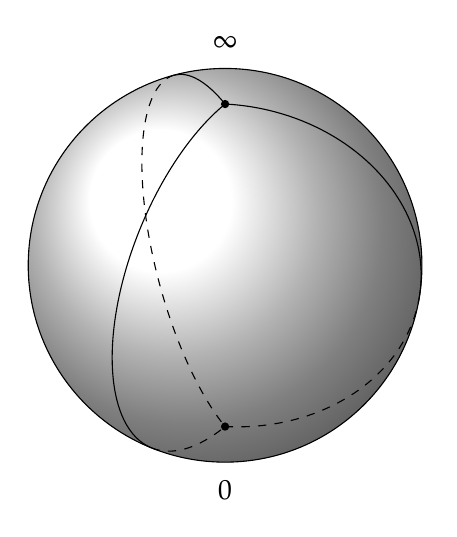
\begin{tikzpicture}[baseline=(current bounding box.center)]

\newcommand\pgfmathsinandcos[3]{%
  \pgfmathsetmacro#1{sin(#3)}%
  \pgfmathsetmacro#2{cos(#3)}%
}
\newcommand\LongitudePlane[3][current plane]{%
  \pgfmathsinandcos\sinEl\cosEl{#2} % elevation
  \pgfmathsinandcos\sint\cost{#3} % azimuth
  \tikzset{#1/.style={cm={\cost,\sint*\sinEl,0,\cosEl,(0,0)}}}
}
\newcommand\DrawLongitudeCircle[2][1]{
  \LongitudePlane{35}{#2} % first argument is angle of elevation
  \tikzset{current plane/.prefix style={scale=#1}}
   % angle of "visibility"
  \pgfmathsetmacro\angVis{atan(sin(#2)*cos(35)/sin(35))} % these are angle of elevation too
  % this might assume that the angle of elevation is positive
  \draw[current plane] (\angVis:1) arc (\angVis:90:1);
  \draw[current plane,dashed] (\angVis:1) arc (\angVis:-90:1);
}

% the "2.5" magic number is the radius of the sphere 
% the "35" magic number is the angle of elevation of the camera
\pgfmathsetmacro\H{2.5*cos(35)}
\filldraw[ball color=white] (0,0) circle (2.5);
\foreach \t in {-5,-125,-245} { \DrawLongitudeCircle[2.5]{\t} }
\coordinate[style={inner sep=0pt,outer sep=0pt,minimum size=3pt,
    fill=black,circle}] (O) at (0,-\H);
\node[below=16pt] at (O) {$0$};
\coordinate[style={inner sep=0pt,outer sep=0pt,minimum size=3pt,
    fill=black,circle}] (I) at (0,\H);
\node[above=16pt] at (I) {$\infty$};
\end{tikzpicture}
\end{center}

\caption{The period map at $n = 2$, $p = 2$}
\end{figure}

\begin{theorem}\citeme{\cite{HopkinsGrossAnnouncement,StricklandGHDuality}}
\todo{Make sure you get this right.}
The sheaf $\context{E_\Gamma}(\mathbb I_{\Q/\Z})$ is the dualizing sheaf on $(\moduli{fg})^\wedge_\Gamma$. \qed
\end{theorem}





\section{Knowns and unknowns}



\subsection*{Higher orientations}

$\TAF$ and friends\label{TAFDiscussion}

The $\alpha_{1/1}$ argument: Prop 2.3.2 of Hovey's $v_n$--elements of ring spectra

% The HLP calculations

\subsection*{Equivariance}

This is tied up with the theory of power operations in a way I've never really thought about.  Seems complicated.

You should also mention the ``rigidity'' of the elliptic genus, which is about an $S^1$--equivariant version.

\subsection*{Index theorems}

Connections with analysis

The Stolz--Teichner program








-----

Contexts for structured ring spectra

Difficulty in computing $\S_d \actson E_d^*$. (Gross--Hopkins and the period map.)

Barry's $p$--adic measures

Fixed point spectra and e.g. $L_{K(2)} \tmf$.

Blueshift, A--M--S, and the relationship to A--F--G?

Does $E_n$ receive an $E_\infty$ orientation?  Does $BP$?

Remark 12.13 of published $H_\infty$ AHS says their obstruction framework agrees with the $E_\infty$ obstruction framework (if you take everything in sight to have $E_\infty$ structures).  This is almost certainly related to the discussion at the end of Matt's thesis about the $MU$--orientation of $E_d$.\todo{Section 12.4 compares doing $H_\infty$ descent with doing $E_\infty$ descent and shows that they're the same (in the case of interest?).}

Hovey's paper on $v_n$--periodic elements in ring spectra.  He has a nice (and thorough!) exposition on why one should be interested in bordism spectra and their splittings: for instance, a careful analysis of $M\Spin$ will inexorably lead one toward studying $KO$.  It would be nice if studying $M\String$ (and potentially higher analogues) would lead one toward non-completed, non-connective versions of $EO_n$.  Talk about $BoP$, for instance.

Matt's short resolutions of chromatically localized $MU$.






\backmatter

\renewcommand\chaptername{\relax}

\bibliographystyle{alpha}
\bibliography{main}



\cleardoublepage
\printindex



% --- REMOVE ME EVENTUALLY ---

\newpage

Number of to-dos used: \thetodocounter

% --- END REMOVE ME EVENTUALLY ---



\end{document}
